% ****************************************************************************************** % Dissertation template and document class for Princeton University
% Author  : Jeffrey Scott Dwoskin <jdwoskin@princeton.edu>
% Adapted from: http://www.math.princeton.edu/graduate/tex/puthesis.html
% ****************************************************************************************** %


%%% For print copies
%% set 'singlespace' option to set entire thesis to single space, and define "\printmode" to remove all hyperlinks for printed copies of the thesis. Delete all output files before changing this mode -- it will turn hyperref package on and off
% \documentclass[12pt,lot, lof, singlespace]{puthesis}
% \newcommand{\printmode}{}

%%% For the electronic copy, use doublespacing, define "\proquestmode" to use outlined links, instead of colored links. 
\documentclass[12pt,lot, lof]{puthesis}
% \newcommand{\proquestmode}{}
% I prefer proquestmode to be off for electronic copies for normal use, since the colored links are less distracting. However when printed in black and white, the colored links are difficult to read. 

%%% For early drafts without some of the frontmatter
% Also see the "ifodd" command below to disable more frontmatter
%\documentclass[12pt]{puthesis}

%%%%%%%%%%%%%%%%%%%%%%%%%%%%%%%%%%%%%%%%%%%%%%%%%%%%%%%%%%%%%\
%%%% Author & title page info

\title{Manifold Learning for States and Parameters}

\submitted{September 2017}  % degree conferral date (January, April, June, September, or November)
\copyrightyear{2017}  % year in which the copyright is secured by publication of the dissertation.
\author{Alexander Holiday}
\adviser{Professor Ioannis G. Kevrekidis}  %replace with the full name of your adviser
%\departmentprefix{Program in}  % defaults to "Department of", but programs need to change this.
\department{Chemical and Biological Engineering}

%%%%%%%%%%%%%%%%%%%%%%%%%%%%%%%%%%%%%%%%%%%%%%%%%%%%%%%%%%%%%\
%%%% Tweak float placements
% From: http://mintaka.sdsu.edu/GF/bibliog/latex/floats.html "Controlling LaTeX Floats"
% and based on: http://www.tex.ac.uk/cgi-bin/texfaq2html?label=floats
% LaTeX defaults listed at: http://people.cs.uu.nl/piet/floats/node1.html

% Alter some LaTeX defaults for better treatment of figures:
    % See p.105 of "TeX Unbound" for suggested values.
    % See pp. 199-200 of Lamport's "LaTeX" book for details.
    %   General parameters, for ALL pages:
    \renewcommand{\topfraction}{0.85}	% max fraction of floats at top
    \renewcommand{\bottomfraction}{0.6}	% max fraction of floats at bottom
    %   Parameters for TEXT pages (not float pages):
    \setcounter{topnumber}{2}
    \setcounter{bottomnumber}{2}
    \setcounter{totalnumber}{4}     % 2 may work better
    \setcounter{dbltopnumber}{2}    % for 2-column pages
    \renewcommand{\dbltopfraction}{0.66}	% fit big float above 2-col. text
    \renewcommand{\textfraction}{0.15}	% allow minimal text w. figs
    %   Parameters for FLOAT pages (not text pages):
    \renewcommand{\floatpagefraction}{0.66}	% require fuller float pages
	% N.B.: floatpagefraction MUST be less than topfraction !!
    \renewcommand{\dblfloatpagefraction}{0.66}	% require fuller float pages

% The documentclass already sets parameters to make a high penalty for widows and orphans. 

%%%%%%%%%%%%%%%%%%%%%%%%%%%%%%%%%%%%%%%%%%%%%%%%%%%%%%%%%%%%%\
%%%% Use packages

%\usepackage{amsfonts}

%%% For figures
% \usepackage{graphicx}
\usepackage[draft]{graphicx}
\graphicspath{
  {./ch-intro/figs/}
  {./ch-graphs/figs/}
  {./ch-sis/figs/}
  {./ch-params/figs/}}
%\usepackage{subfig,rotate}
\usepackage{subcaption}

\DeclareCaptionSubType[Alph]{figure}
\captionsetup[subfigure]{labelformat=simple, font=sf}

% for chemistry arrows
\usepackage{chemarr}

% for nice arrays
\usepackage{blkarray}

\usepackage{epstopdf}

%%% for comments
\usepackage{verbatim}

%%% For tables
\usepackage{multirow}
% Longtable lets you have tables that span multiple pages.
\usepackage{longtable}

% Booktabs produces far nicer tables than the standard LaTeX tables.
%   see: http://en.wikibooks.org/wiki/LaTeX/Tables
\usepackage{booktabs}

%set parameters for longtable:
% default caption width is 4in for longtable, but wider for normal tables
\setlength{\LTcapwidth}{\textwidth}


%% For math
\usepackage{amsmath, amsfonts, amssymb}
\DeclareMathOperator*{\argmin}{arg\,min}

\usepackage[sort]{natbib}

%% notation
\def \data {\mathbf{y}}
\def \dataone {y}
\def \measfn {\mathbf{f}}
\def \ndata {m}
\def \lowdim {d}
\def \lowdimslow { {d_1} }
\def \highdim {n}
\def \rotdim {d_{rot}}
\def \dmeps {\sigma_{kernel}}
\def \manifold {\mathcal{M}_\lowdim}

\def \chap {Chapter}
\def \fig {Figure}
\def \sec {Section}
\def \app {Appendix}
\def \tab {Table}

%%%%%%%%%%%%%%%%%%%%%%%%%%%%%%%%%%%%%%%%%%%%%%%%%%%%%%%%%%
%%% Printed vs. online formatting
\ifdefined\printmode

% Printed copy
% url package understands urls (with proper line-breaks) without hyperlinking them
\usepackage{url}
\usepackage[hidelinks]{hyperref}
%\usepackage[top=1in,left=1.5in,bottom=1in,right=1in,footskip=0.25in]{geometry}

\else

\ifdefined\proquestmode
%ProQuest copy -- http://www.princeton.edu/~mudd/thesis/Submissionguide.pdf

% ProQuest requires a double spaced version (set previously). They will take an electronic copy, so we want links in the pdf, but also copies may be printed or made into microfilm in black and white, so we want outlined links instead of colored links.
\usepackage{hyperref}
\hypersetup{bookmarksnumbered}

%\usepackage[top=1in,left=1in,bottom=1in,right=1in,footskip=0.25in]{geometry}
\oddsidemargin 0in   %{.4375in}
\textwidth 6.5in

% copy the already-set title and author to use in the pdf properties
\makeatletter
\hypersetup{pdftitle=\@title,pdfauthor=\@author}
\makeatother

\else
% Online copy

% adds internal linked references, pdf bookmarks, etc

% turn all references and citations into hyperlinks:
%  -- not for printed copies
% -- automatically includes url package
% options:
%   colorlinks makes links by coloring the text instead of putting a rectangle around the text.
\usepackage{hyperref}
\hypersetup{colorlinks,bookmarksnumbered}

% copy the already-set title and author to use in the pdf properties
\makeatletter
\hypersetup{pdftitle=\@title,pdfauthor=\@author}
\makeatother

% make the page number rather than the text be the link for ToC entries
%\hypersetup{linktocpage}
\fi % proquest or online formatting
\fi % printed or online formatting


%%%%%%%%%%%%%%%%%%%%%%%%%%%%%%%%%%%%%%%%%%%%%%%%%%%%%%%%%%%%%\
%%%% Define commands

% Define any custom commands that you want to use.
% For example, highlight notes for future edits to the thesis
%\newcommand{\todo}[1]{\textbf{\emph{TODO:}#1}}

% minus sign be better
\newcommand{\minus}{\scalebox{0.75}[1.0]{$-$}}

% create an environment that will indent text
% see: http://latex.computersci.org/Reference/ListEnvironments
% 	\raggedright makes them left aligned instead of justified
\newenvironment{indenttext}{
    \begin{list}{}{ \itemsep 0in \itemindent 0in
    \labelsep 0in \labelwidth 0in
    \listparindent 0in
    \topsep 0in \partopsep 0in \parskip 0in \parsep 0in
    \leftmargin 1em \rightmargin 0in
    \raggedright
    }
    \item
  }
  {\end{list}}

% another environment that's an indented list, with no spaces between items -- if we want multiple items/lines. Useful in tables. Use \item inside the environment.
% 	\raggedright makes them left aligned instead of justified
\newenvironment{indentlist}{
    \begin{list}{}{ \itemsep 0in \itemindent 0in
    \labelsep 0in \labelwidth 0in
    \listparindent 0in
    \topsep 0in \partopsep 0in \parskip 0in \parsep 0in
    \leftmargin 1em \rightmargin 0in
    \raggedright
    }

  }
  {\end{list}}


% define math shortcuts
\newcommand{\xb}{\mathbf{x}}
\newcommand{\mub}{\pmb{\mu}}
\newcommand{\R}{\mathbb{R}}
\newcommand{\la}{\lambda}
\newcommand{\Li}{\mathbf{L}}
\newcommand{\Res}{\mathbf{R}}

%%%%%%%%%%%%%%%%%%%%%%%%%%%%%%%%%%%%%%%%%%%%%%%%%%%%%%%%%%%%%\
%%%% Front-matter

% For early drafts, you may want to disable some of the frontmatter. Simply change this to "\ifodd 1" to do so.
\ifodd 0
% front-matter disabled while writing chapters
\renewcommand{\maketitlepage}{}
\renewcommand*{\makecopyrightpage}{}
\renewcommand*{\makeabstract}{}

% you can just skip the \acknowledgements and \dedication commands to leave out these sections.

\else


\abstract{
% Abstract can be any length, but should be max 350 words for a Dissertation for ProQuest's print indicies (150 words for a Master's Thesis) or it will be truncated for those uses.
% !TEX root = thesis.tex

Recent decades have seen a tremendous rise in the affordability and
performance of various computational technologies, enabling
researchers to propose and probe ever more complicated numerical
models. These simulations often generate incredible quantities of data
that must be sifted through to glean useful conclusions. This thesis
highlights our efforts to automate this process in two specific areas:
(a) uncovering simplified descriptions of dynamic network models and
(b) detecting important parameter combinations in general nonlinear
systems. Both advances involve modification of the manifold learning algorithm, Diffusion Maps (DMAPS), to
address the particular problem.

In the first case, the challenge is quantifying the similarity of two
networks in a reasonable amount of computational time. We propose a
number of possible solutions, and examine their performance when
combined with DMAPS. We find that by combining suitable measures of
similarity with DMAPS we are able to uncover low-dimensional structure
in a set of networks, thus enabling us to describe the system in terms
of one or two values instead of thousands.

In the second, we must extend Diffusion Maps to operate on the graph
of a function. In particular we consider a model that maps parameter
values to some output. By properly formulating the DMAPS kernel, we enable DMAPS to discover the directions
in parameter space along which model predictions vary most
significantly.

Both result in algorithms that we hope are practically useful to
researchers in a variety of fields who are looking for simplified
descriptions of their complex systems.

}

\acknowledgements{
%I would like to thank...
% !TEX root = thesis.tex

Just as a thesis would be nothing without the graduate student, a graduate student would be nothing without the support of surrounding friends, family and collaborators. My five years have been blessed with a tremendous collection of all three.

To begin, I thank my parents for their constant support. I marvel at their ability to produce the perfect words of encouragement in good times and bad, brightening the joyful days and smoothing over rocky patches along the path. I cannot imagine navigating this journey without your love and guidance behind me, thank you both for all you have done. And thanks to my brothers, Lucas and Jacob, for being most excellent. I cherish the time we spent together, whether in New York or Toronto.

Next, I thank my advisor, Professor Kevrekidis, who has had the most direct influence on the work that follows. I am grateful for the generosity and compassion he displayed throughout our time together, from the many wonderful meals hosted at ``The Spaniard's'', to his emphasis of family over work, encouraging us to return home during difficult times. I will try to emulate his empathy in my future positions.

Continuing in the academic direction, my collaborator and friend Antonios Zagaris is directly responsible for much of Chapter~\ref{ch:params} and I am very thankful for his input over the past two years. He has been a faithful mentor and source of encouragement, and I have enjoyed equally our discussions on the origins of sloppy models as those on the origins of punk rock. Mahdi Kooshkbaghi was also a great help in the final stages of the project, and I regret that our time together was so short. In just six months he became a close friend, introducing me to proper black tea and Kayhan Kalhor. I will miss them both.

My companions in room ACE44 have ensured that the typical day of research was supplemented with DMAPS jokes and off-topic soccer conversations. From the post-docs: Matt Williams taught me good C programming and talked me into my first 5k. Minseok Choi significantly improved my tennis forehand and showed me the best Korean fried-chicken restaurants around. And Juan Bello-Rivas provided excellent Python packages and had many fruitful suggestions on particular aspects of my work. Of the slew of German visiting students: Robert H\"{o}lzel rekindled my love for chess, Felix Kemeth instituted group lunch days, and Felix Dietrich played an instrumental role in designing the lab coffee grinder. From the collection of fellow graduate students: Karthik Rajendran introduced me to many fundamental topics in our group, Carmeline D'Silva helped me navigate the middle of my graduate student career, Dave Sroczynski was a source of fun both inside and outside of the office, Wendy Jiang kindly obliged the occasional conversation in broken Chinese, and I enjoyed discussing the merits of wood versus bamboo cutting boards with Thomas Thiem.

Outside of academics I was fortunate to enjoy time with a close group of classmates. Dmitry Pozharskiy not only worked across from me for four years, but was also an exellent room-mate throughout. Despite my inability to clean any sort of dish in a reasonable timeframe, I could always depend on his support in matters both professional and private; many hours were passed simply chatting on the sidewalk outside our apartment. Tom Bertalan was an office-mate and friend who would never hesitate to offer his help, be it programming advice or a ride to the airport. Yogesh Goyal and I shared many Indian dinners together, and I appreciate the genuine encouragment he has provided over the years. Will Mulhearn was the easy-going and flexible host of many of our evenings who always welcomed new adventures, including a particularly patriotic roadtrip to Canada. Yile Gu brightened the atmosphere of all our events with his cheerfulness, and was the source of our group's most memorable quotes. Together, the six of us travelled across Europe, organized frequent summer barbeques, and played many hours of board games; I am so grateful for their friendship.

There were numerous others whose company I am thankful for. Zach Domach for being my SCUBA buddy and for the many orchestra outtings, Logan Matthews for many good discussions on religion, Ting Chen for being a caring friend and motivated workout buddy, Elia Altabet for many evenings of conversation over whiskey, Clark Chen and Jack Lu for introducing me to the joys of hot-pot and Rai Rai Ramen, Mike Siedlik for consistently attending our badminton games, and Granton Jindal for fun games of tennis, ping pong and soccer.

To those above and the many others who so enriched the past five years: thank you.
}

\dedication{Mum and dad}

\fi  % disable frontmatter


%%%%%%%%%%%%%%%%%%%%%%%%%%%%%%%%%%%%%%%%%%%%%%%%%%%%%%%%%%%%%\
%%%% Hide some chapters

%%% If you want to produce a pdf that includes only certain chapters, specify them with includeonly, in addition to including all chapters below.
%\includeonly{ch-intro/chapter-intro}
%%% You can also specify multiple chapters.
%\includeonly{ch-intro/chapter-intro,ch-drosophila/chapter-drosophila}
%\includeonly{chap1,chap2,chap3}


%%%%%%%%%%%%%%%%%%%%%%%%%%%%%%%%%%%%%%%%%%%%%%%%%%%%%%%%%%%%%
%%%% Notes:

% Footnotes should be placed after punctuation.\footnote{place here.}
% Generally, place citations before the period~\cite{anotherauthor}.
% The proper usage for i.e., and e.g., include commas ``(e.g., option A, option B)''

%%%%%%%%%%%%%%%%%%%%%%%%%%%%%%%%%%%%%%%%%%%%%%%%%%%%%%%%%%%%%
%%%% Import chapters

\begin{document}

\makefrontmatter


% If you've disabled frontmatter, you can insert the toc manually
%\tableofcontents\clearpage

% \include lets us split up the document (and each include starts a new page):
\chapter{Introduction\label{ch:intro}}

Machine learning has been used in a vast array of contexts. Principal
component analysis has been used to analyze PET scans \cite{Functional
  Connectivity: The Principal-Component Analysis of Large (PET) Data
  Sets}, to predict traffice flow \cite{Forecasting Approach for
  Short-term Traffic Flow based on Principal Component Analysis and
  Combined Neural Network}, and to examine groundwater composition
\cite{Temporal evolution of groundwater composition in an alluvial
  aquifer (Pisuerga River, Spain) by principal component analysis},
among an array of other novel applications \cite{Principal component
  analysis of molecular dynamics: On the use of Cartesian vs. internal
  coordinates; Monitoring batch processes using multiway principal
  component analysis; Forecasting Using Principal Components From a
  Large Number of Predictors}. 

% % possible first sentences of thesis

% The following chapters are a test of the theory that engineering
% theses are never read, neither by their advisor nor original
% author. Instead, the theory asserts that the author vomits the
% document into existence in a violent storm of anxiety and
% anticipation, never to be perused again.

% There are those that do brave battle with the big data and there are
% those that survey the wasted battlefield, strewn with broken
% algorithms and bad statistics, and run towards the siren sound of
% Excel. But there is no escape. Some of the warrior's
% deeds were recorded so that future generations would know the folly of
% csv files; the following documents were recovered from the battlefield
% of nonlinearities. Let them be a lesson to all.

% It is not uncommon for the modern researcher to pore over his
% gigabytes of data and question what it is all for.

% Should your data remain big for over six hours after reading this
% thesis, please consult your nearest graduate student.

% Modern researchers are often confronted by the unnecessarry bigness
% of their datasets and wish to make them smaller. This can occur for a
% variety of reasons. 

% Despite growing demand for algorithms that work good, scientists
% are unable to make them good.

% It is no secret that big data requires big algorithms.

\section{Outline of thesis}

We begin with a background of the mathematical techniques used
throughout the bulk of the thesis work, including manifold learning
algorithms and the Equation Free framework. With this foundation
established, we turn to an extension of these techniques into the
field of network science. In particular, we study a dynamic multigraph
model which exhibits the sort of preferential attachment phenomenon
seen in many real-world social networks. We implement a coarse
projective integrator for this system and use it to construct a
stationary state solver. We also explore the problem of quantifying
similarities between pairs of networks, and having found such a
measure we embed whole trajectories of network evolution and find
low-dimensional structure. 

After validating the use of manifold learning in this simpler network
setting, we apply similar techniques to a popular model of disease
propogation, the susceptible-infected-susceptible (SIS) model. Again,
by selecting an appropriate measure of similarity between networks we
are able to algorithmically reduce the problem's dimensionality using
DMAPS without recourse to analytical derivations. Our results suggest
that a previously-derived low dimensional system may be improved.

The third and final section of this thesis moves from network models
to more traditional systems of ordinary differential equations whose
evolution is governed by certain sets of parameters. Here, the goal is
to determine which parameters have the largest influence on model
predictions so that we may ignore those parameter combinations that do
not significantly affect the model output, thus reducing the
dimensionality of parameter space. By constructing a variant of DMAPS
that operates on model predictions, we are able to realize this
objective even in the presence of nonlinear parameter combinations. In
a related section, we also show how such an approach can identify the
fast manifolds in singularly perturbed systems.

In total, these chapters display the utility of extending manifold
learning techniques into novel domains, and of the pervasiveness of
low-dimensional structure in complex
systems.

%%% Local Variables: ***
%%% mode:latex ***
%%% TeX-master: "../../thesis.tex"  ***
%%% End: ***
\section{Manifold learning techniques\label{sec:ml}}

Since the advent of principal component analysis (PCA) in 1933
\ref{hotelling}, manifold learning has been applied to a wide array of
problems in an effort to unearth hidden structure in data. In a
typical setting, a researcher will collect many data points
$\{x_i\}_{i=1}^N$, often vectors in $\mathbb{R}^n$, that contain
features relevant to the problem under investigation. For example,
when studying collections of $k \times k$-pixel images, it is common
to stack each column of pixel values so that the dataset becomes
vectors $x_i \in \mathbb{R}^n$ where $n = k^2$. Alternatively, when
studying a certain population, each $x_i$ couuld represent a
collection of features about a particular individual such as their
income, education level, and age: a vector in $\mathbb{R}^3$. Manifold
learning would then be applied to this collection of points to reveal
structure in the data that might be obscured by its
high-dimensionality. 

In the latter example, one would expect to find
that income and education level are not indepedent variables, but are
instead positively correlated. This is unsurprising, and hardly a good
use-case for manifold learning. On the other hand, if we study a
collection of images of a human face, each taken at a different angle,
manifold learning can uncover that each image can be described by just
two variables hidden in the dataset: the azimuthal and polar angle at
which the photo was taken \ref{dmaps or isomap}. This example
demonstrates the power of manifold learning as a form of
dimensionality reduction: we can now describe each image as $y_i =
\begin{bmatrix} \theta_i \\ \phi_i \end{bmatrix} \in \mathbb{R}^2$
instead of $x_i \in \mathbb{R}^{4096}$ (if the image contains
$64 \times 64 = 4096$ pixels).  Equivalently, we could say that
$x \in \mathbb{R}^{4096}$ is parameterized by $y = \begin{bmatrix}
  \theta \\ \phi \end{bmatrix} \in \mathbb{R}^2$.

Many approaches have been proposed to address this problem, each
exploiting a different aspect of the dataset. Some are designed to
find linear relationships among input variables \ref{PCA}, others use
the smoothness of the manifold as a basis for a new parameterization
\ref{hessiang eigenmaps}. Below, we detail the mathematical
underpinnings of two particular methods: PCA and Diffusion Maps
(DMAPS). As the most widely used manifold learning technique, PCA is
conceptually simple and provides easily-understandable
results. However, we will see that it is incapable of efficiently
embedding nonlinear manifolds. For this, we turn to DMAPS, a method
that will return a better embedding of the data at the cost of
interpretability. Both are used throughout subsequent sections of this
paper.

\subsection{Principal component analysis\label{sec:pca}}

In brief, PCA returns a ranking of the important linear relationships
in data. This importance is determined by the amount of the data's
variability a particular linear relationship is able to capture. These
statements are made precise below.

As usual we begin with a collection of $N$ vectors $x_i \in \mathbb{R}^n$,
which we stack in rows to form our input matrix

\begin{align}
  X = \begin{bmatrix} \; - \; x_1^T \; - \; \\ \; - \; x_2^T \; - \; \\ \vdots \\ \; - \; x_N^T
    \; - \; \end{bmatrix} \in \mathbb{R}^{N \times n}
\end{align}

Note that each column represents a particular variable, e.g. age or
income, while each row contains an individual data point. We will
assume that each column has a mean value of zero; if not the mean can
simply be subtracted from each column. We will also assume that we
$N \gg n$, so one imagine can running many experiments in which only a
few variables are measured each time. \\

The problem can now be posed as: if we projected each $x_i$ along some
$v \in \mathbb{R}^n$, which choice of $v$ would maximize the variance
in the projection? More formally, we wish to solve

\begin{align}
  \max_{v \in \mathbb{R}^n} \mathrm{var}(Xv) = v^TX^TXv \\
  \mathrm{s.t.} \| v \| = 1
\end{align}

where we have added the scaling condition $\| v \| = 1$ to prevent
infinite variances. An equivalent formulation is

\begin{align}
  \max_{v \in \mathbb{R}^n} \frac{v^TX^TXv}{v^Tv}
\end{align}

where we notice that $\frac{v^TX^TXv}{v^Tv}$ is the Rayleigh quotient
of $M = X^TX$. It is well known that the Rayleigh quotient is
maximized when $v$ is the eigenvector of $M$ corresponding to the
largest eigenvalue. Thus if we order the eigenvalues
$\lambda_1, \lambda_2, \cdots, \lambda_n$ and corresponding
eigenvectors $v_1, v_2, \cdots, v_n$ such that
$\lambda_i \ge \lambda_{i+1}$, we find that $v_1$ is our desired
vector. Note that this makes some intuitive sense as $M = X^TX$ is the
unscaled covariance matrix of $X$, and by choosing the largest
eigenvector of $X^TX$, we are choosing the direction along which
variance is maximized. \\

There is a clear connection between PCA and the singular value
decomposition (SVD) of a matrix, and the two terms are often used
interchangeably. The SVD, which exists for every
$X \in \mathbb{R}^{N \times n}$, is given by

\begin{align}
  X = U D V^T =   
  \begin{bmatrix}
    & & & \\ 
    | & | &  & |  \\
    u_1 & u_2 & \cdots & u_n \\
    | & | &  & |  \\
    & & &  \\
  \end{bmatrix}
  \begin{bmatrix} 
    \sigma_1^2 & & & \\
    & \sigma_2^2 & & \\
    & & \ddots & \\
    & &  & \sigma_n^2 \\
  \end{bmatrix}
  \left[ \begin{array}{ccccc}
           - & \multicolumn{3}{c}{v_1} & - \\
           - & \multicolumn{3}{c}{v_2} & - \\
             & & \vdots & & \\
           - & \multicolumn{3}{c}{v_n} & - \\
         \end{array} \right]
\end{align}

where $U$ and $V$ are $N \times n$ and $n \times n$ unitary matrices,
and $D$ is an $n \times n$ diagonal matrix with non-negative
entries. Now $X^TX$ becomes

\begin{align}
  X^T X = (V D^T U^T) U D V^T = V D^2 V^T
\end{align}

This shows that the vector $v_1$ is the very same vector we desire
from our principal component analysis: the top eigenvector of the
unscaled covariance matrix.

To actually affect any dimensionality reduction, we would use a subset
of these principal components to project our data into some reduced
number of dimensions. For instance, if $\hat{V}$ is an $n \times k$
matrix containing the leading $k$ singular vectors of $X$, we would
have

\begin{align}
  y_i = \hat{V}\hat{V}^T x_i
\end{align}

corresponding to a reduction in dimensionality from $n$ to $k$.

\subsubsection{Example}

As a concrete example, and to further cement the statistical aspects
of the technique, consider drawing points $x_1$ and $x_2$ from a
multivariate normal distribution. Let them share a mean value of zero
and a variance of one, but let their covariance be two. Thus

\begin{align}
  \mu_1 &= \mu_2 &= 0 \\
  \Sigma_{11} &= \Sigma_{22} &= 4.5 \\
  &\Sigma_{12} &= 5.5
\end{align}

If $\xb = (x_1, x_2)$, $\xb \sim \mathcal{N}(\mub, \Sigma)$ with
$\mub = (\mu_1, \mu_2)$ and $\Sigma = \begin{bmatrix} \sigma_{11}^2 &
  \sigma_{12}^2 \\ \sigma_{12}^2 &
  \sigma_{22}^2 \end{bmatrix}$. Taking the eigendecomposition of
$\Sigma$ we find

\begin{align}
  V = \begin{bmatrix} 1/\sqrt{2} & 1/\sqrt{2} \\
    1/\sqrt{2} & - 1/\sqrt{2} 
  \end{bmatrix} \quad \mathrm{and} \quad
                 \Sigma = \begin{bmatrix} 10 & 0 \\
                   0 & 1 
                 \end{bmatrix}
\end{align}

This, then, would be the expected result of our principal component
analysis: a vector pointing in the $(1,1)$ direction with a
corresponding singular value of $\sqrt{10 n}$, and a second vector pointing in
$(1, -1)$ with singular value $\sqrt{1 n}$ where $n$ is the number of
points in our sample. Fig. \ref{fig:pca-ex} shows a
sample dataset chosen from this particular distribution, along with
principal component vectors scaled by their singular values. The
result is as expected. Indeed, inspecting the numerical output from
5000 points we find

\begin{align}
  V \approx \begin{bmatrix} 1/\sqrt{2} & 1/\sqrt{2} \\
    1/\sqrt{2} & - 1/\sqrt{2} 
  \end{bmatrix} \quad \mathrm{and} \quad
                 \Sigma = \begin{bmatrix} 222 \approx \sqrt{50000} & 0 \\
                   0 & 71 \approx \sqrt{5000}
                 \end{bmatrix}
\end{align}

\begin{figure}
  \centering
  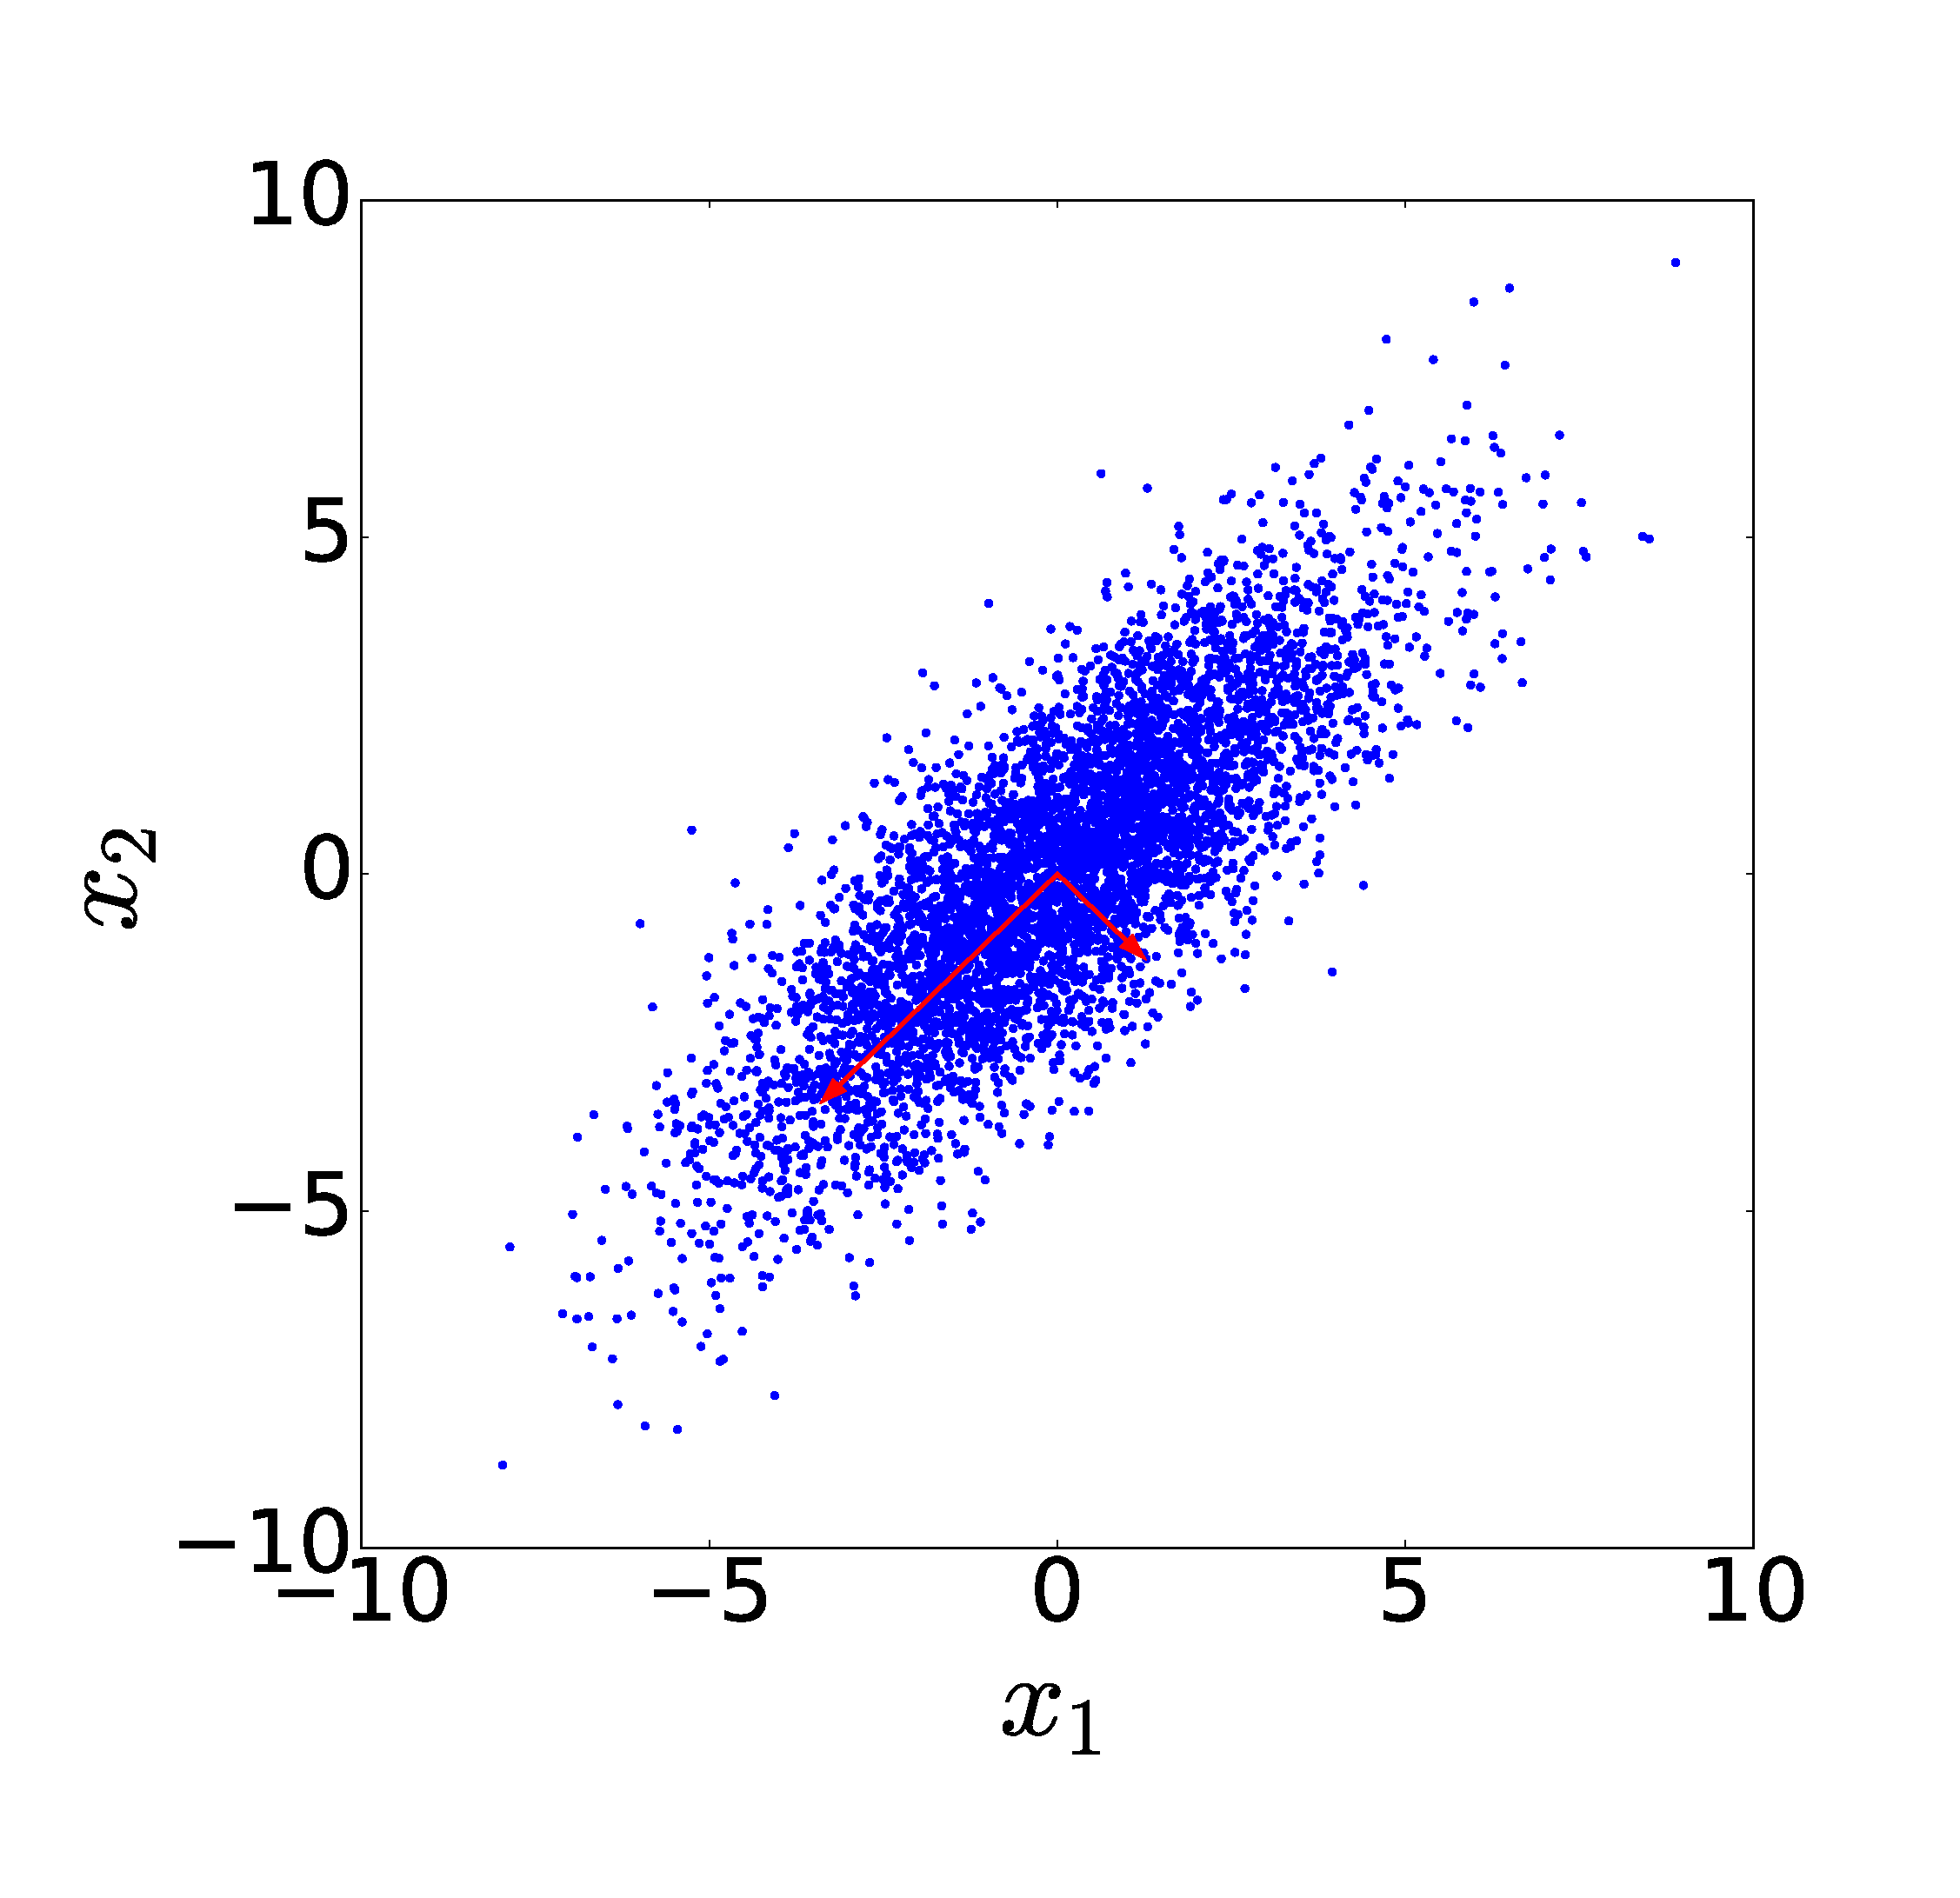
\includegraphics[width=0.8\textwidth]{pca-ex}
  \caption[Example of principal component analysis]{Principal
    components found through PCA on the blue point cloud, scaled by
    singular value. \label{fig:pca-ex}}
\end{figure}

Besides its relative simplicity and ease of implementation, PCA has
one other great strength compared to other dimensionality reduction
methods: it provides an explicit functional form between the input
variables and the output projection in the form of a simple, linear
relationship. In the context of PCA, the principal vectors, which are
some linear combination of the input variables, are precisely the
``best'' new variables to work in. Using the output of the previous
example, we may decide that only the value $x_1 + x_2$ is important
enough to keep, allowing us to reduce our description of the dataset
from $(x_1, x_2) \rightarrow (x_1 + x_2)$. As we will see in the
following section, while more complex methods offer distinct
advantages over PCA, they lack such easily interpretable results.

\subsection{Diffusion Maps \label{sec:dmaps}}

While PCA may be effective in uncovering linear relationships among
input variables, most real-world problems exhibit significant
nonlinearities. This motivates our introduction of Diffusion Maps
(DMAPS), an algorithm designed to address such difficulties. We begin
with a description of the DMAPS' implementation.

The goal of DMAPS is identical to that of PCA: given some dataset
$\{x_1, x_2, \hdots, x_N \}$ with $x_i \in \R^n$, we desire a mapping
of $x_i$ into $y_i$ such that $y_i$ is a low-dimensional embedding of
$x_i$ that captures important characteristics of the original data. We
again stack each datapoint $x_i$ into an $N \times n$ matrix
$X$. DMAPS begins by evaluating a Gaussian kernel between each point,
and storing the results in an $N \times N$ matrix $W$, so that

\begin{align}
  W_{ij} = \exp \left( -\frac{\|x_i - x_j\|^2}{\epsilon^2} \right)
\end{align}

where $\epsilon$ is a parameter which will be discussed below. Note
that $W_{ij} \rightarrow 0$ as the distance between $x_i$ and $x_j$
increases. We then calculate the sum of each row of $W$, and use these
values to construct a new diagonal matrix $D$ with
$D_{ii} = \sum_j W_{ij}$. Finally, we compute $A = D^{-1} W$. As
$A_{ij} \ge 0$ and $\sum_j A_{ij} = 1$, $A$ is a stochastic
matrix. This lends its entries $A_{ij}$ an intuitive interpretation:
if we are performing a random walk from point to point in our dataset,
$A_{ij}$ is the probability that, starting from $x_i$ we will hop next
to $x_j$. Just as $W_{ij}$ decreases when the distance between $x_i$
and $x_j$ grows, so too will $A_{ij}$ decrease, so that the
probability of jumping to nearby points is much greater than the
probability of jumping to distant ones. This concept is illustrated in
Fig.~\ref{fig:dmaps-3pts} for three points.

\begin{figure}
  \centering
  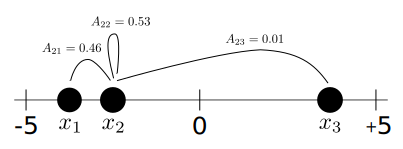
\includegraphics[width=0.8\textwidth]{dmaps-3pts}
  \caption[Illustration of random walk on data]{Probability of
    transitioning from $x_1$ to points $x_2$ and $x_3$ and to
    itself. \label{fig:dmaps-3pts}}
\end{figure}


Having constructed the stochastic matrix $A$, the penultimate step in
the DMAPS algorithm is to perform an eigen-decomposition of
$A$. Numerically, it is helpful to note that $A$ is similar to the
symmetric matrix $\hat{A}$

\begin{align}
  \hat{A} &= D^{1/2}A D^{-1/2} \\
  & = D^{-1/2} W D^{-1/2}
\end{align}

As specialied eigensolvers such as the Lanczos algorithm have been
developed for symmetric matrices, it is best to transform $A$ into
$\hat{A}$, calculate the eigendecomposition, and transform the
eigenvectors of $\hat{A}$ into eigenvectors of $A$ by multiplying by
$D^{-1/2}$. This results in eigenvalues
$\la_0 \ge |\la_1| \ge \cdots \ge |\la_{n-1}|$ with $\la_0 = 1$ and
corresponding eigenvectors $\phi_0, \phi_1, \cdots, \phi_{n-1}$. That
all eigenvalues have absolute value no greater than one is a
consequence of Gershgorin's circle theorem, while the existence of
$\la_0 = 1$ is clear when one considers the eigenvector $v_0 = (1/N,
1/N, \cdots, 1/N)^T$, so that, for any row stochastic matrix $A$, $A
v_0 = \la_0 v_0$. Finally, the low-dimensional map is given by

\begin{align}
  \Phi_t: x_i \rightarrow \begin{bmatrix} \la_1^t \phi_1(i) \\ \la_2^t
    \phi_2(i) \\ \vdots \\ \la_k^t \phi_k(i) \end{bmatrix} \in \R^k
\end{align}

where we have chosen the top $k \ll N$ eigenvectors to embed our data,
and $\phi_j(i)$ represents the $i$th component of $\phi_j$. It is not
immediately clear what the effect of such a mapping is, but there are
two useful characterizations of the DMAPS embeddings that elucidate
its utility. First, letting $y_i = \Phi(x_i)$, we can show that $y_i$
provides the best $k$-dimensional approximation to the so-called
``diffusion distance'' between points. We now detail this connection.

\subsubsection{Diffusion distance}

Returning to our stochastic matrix $A$, say we have a vector
$\Psi_t \in \R^N$ where each entry $\Psi_t(i)$ represents the
probability of finding a random walk at data point $i$ at step $t$ of
the walk (so $\sum_j \Psi_t(j) = 1$ and $\Psi_t(j) \ge 0$). In other
terms, $\Psi_t(j) = p(r_t = x_j)$ where $r_i$ is the position of the
random walk at iteration $i$. We then have that

\begin{align}
  \Psi_t^T = \Psi_0^T A^t
\end{align}

to see this, note that

\begin{align*}
  \Psi_t^T A = \big( &\sum_i \Psi_t(i) A_{i1},\; \sum_i
                         \Psi_t(i) A_{i2},\; \dots,\; \sum_i \Psi_t(i) A_{iN} \big) \\
             = \bigg( &\sum_i p(r_{t+1} = x_1 | r_t = x_i)p(r_t = x_i) , \\
             & \sum_i p(r_{t+1} = x_2 | r_t = x_i)p(r_t = x_i), \\
             & \dots, \\
                     & \sum_i p(r_{t+1} = x_N | r_t = x_i)p(r_t = x_i)
                       \bigg) \\
  = \bigg( & p(r_{t+1} = x_1), \;p(r_{t+1} = x_2), \; \dots, \;
             p(r_{t+1} = x_N) \bigg) \\
  = & \Psi_{t+1}
\end{align*}

so by multiplying $\Psi_0$ by $A^t$, we march our random walk forward
$t$ steps. In the limit of infinite steps, we find that the
probability distribution becomes stationary, so further applications
of $A$ do not change the probability of being at a particular
point. We will call this stationary distribution $\Psi_*$, and find
that

\begin{align}
  \Psi_*^T &= \lim_{t \rightarrow \infty} \Psi_0^T A^t \\
           &= \Psi_*^T A
\end{align}

Thus $\Psi_*$ is the right eigenvector of $A$ with eigenvalue one. By
inspection, its entries will be $\Psi_*(i) = \frac{d_i}{\sum_j d_j}$
where $d_i = \sum_i A_{ij}$.

We now define the diffusion distance at time $t$ between points $x$
and $y$ to be

\begin{align}
  D^2_t(x_i, x_j) &= \| p(r_t = x_i| \cdot) - p(r_t = x_j | \cdot) \|^2_{1/\Psi_*} \\
                  &= \sum_k \frac{A^t_{ki} - A^t_{kj}}{\Psi_*(k)} \\
\end{align}

Now, denoting the right eigenvectors of $A$ as $\psi_i$, we have
$A^t_{ij} = \sum_k \la_k^t \phi_k(i) \psi_k(j)$ by the spectral
decomposition of $A$. Substituting this into the equation above gives

\begin{align}
  D^2_t(x_i, x_j) &= \sum_{k=1}^{N-1} \la_k^t \left( \phi_k(i) -
                    \phi_k(j) \right)^2 \\
\end{align}

where we omit $k=0$ which corresponds to the constant
eigenvector. Finally, we see that this diffusion distance between
points is approximated by the Euclidean distance between $y_i$ and
$y_j$. As we have chosen the largest $k$ eigenvalues to include in
$y_i$, and assuming the magnitude of the eigenvalues decays quickly
after $\la_k$, we see that

\begin{align}
  D^2_t(x_i, x_j) & \approx \sum_{k=1}^{k} \la_k^t \left( \phi_k(i) -
                    \phi_k(j) \right)^2 \\
  & = \| y_i - y_j \|^2
\end{align}

This provides an interesting probabilisitic interpretation to the
DMAPS embedding. We now turn to a geometric view of the algorithm.

\subsubsection{Eigenfunctions of operators}

Besides embedding points based on their approximate diffusion
distances, DMAPS also provides a parameterization of the manifold on
which the data reside by yielding approximate eigenfunctions of
diffusion operators defined on the manifold. We assume that our data
have been sampled from an underlying manifold $\chi$ with some density
$p(x)$. Essentially, as the number of points tends to infinity and our
$\epsilon$ scaling term tends to zero, the resulting stochastic matrix
$A$ approximates certain differential operators depending on the value
of $\alpha$ in the algorithm. These are given below

\begin{equation}
\begin{aligned}
  \alpha &= 0: &&\frac{(I - A)}{\epsilon} \phi = \Delta \phi + 2
    \nabla \phi \cdot \frac{\nabla p}{p} \\
  \alpha &= 1/2: &&\frac{(I - A)}{\epsilon} \phi = \Delta \phi +
    \nabla \phi \cdot \frac{\nabla p}{p} \\
  \alpha &= 1: &&\frac{(I - A)}{\epsilon} \phi = \Delta \phi
\end{aligned}
\end{equation}

The eigenvectors of $A$ will then approximate the eigenfunctions of
the corresponding operator. In particular, we see that with the choice
$\alpha = 1$, we recover the Laplace-Beltrami operator on our
manifold. As such, the resulting eigenvectors will be influenced only
by the geometry of the manifold and not by our sampling density on
it. However, if our data is uniformly sampled so that $p(x) = c$, all
values of $\alpha $ yield the same result.

We illustrate this result with an analytically tractable example for
which the manifold is a simple rectangle, $\chi = [0, L_x] \times [0,
L_y]$ where $L_x$ and $L_y$ are the lengths of the rectangle along the
$x$ and $y$ axes. We wish to find the eigenfunctions of the Laplace
operator over the rectangle with homogenous Neumann boundary
conditions. That is, we want to find functions $f$ such that $\Delta f
= \lambda f$ and $\frac{\partial f}{\partial x}\Big|_{x=0,L_x}
=\frac{\partial f}{\partial y}\Big|_{y=0,L_y} = 0$. We solve this
problem using separation of variables to obtain

\begin{align}
  f_{ij} = \cos\left(\frac{i \pi x}{L_x}\right) \cos\left(\frac{j \pi y}{L_y}\right) \quad
  \mathrm{and} \quad \lambda_{ij} = -\left( \left(\frac{i \pi
  }{L_x}\right)^2 + \left(\frac{j \pi}{L_y}\right)^2 \right)
\end{align}

Assigning $L_x = \frac{5}{2}$ and $L_y = 1$ and ordering these eigenpairs by
increasing $|\lambda_{ij}|$, we see that the first few eigenfunctions
will be

\begin{itemize}
\item $\lambda_{10} = -\left(\frac{2 \pi}{5}\right)^2$ with $f_{10} =
  \cos \left(\frac{2 \pi x}{5} \right)$
\item $\lambda_{20} = -\left(\frac{4 \pi}{5}\right)^2$ with $f_{20} =
  \cos \left(\frac{4 \pi x}{5} \right)$
\item $\lambda_{01} = -\pi^2$ with $f_{01} =
  \cos \left( \pi y \right)$
\end{itemize}

The key insight is that the maps $x \rightarrow f_{10} (x)$ and
$y \rightarrow f_{01} (y)$ are bijections from the $x$ and $y$ axes
onto eigenfunctions of the diffusion operator. Thus, instead of
describing points on our rectangular manifold by their $(x,y)$
coordinates, they could equivalently be specified by values of
$(f_{10}, f_{01})$. Although $x$ and $y$ may be a more natural way of
parameterizing the rectangle, in high-dimensional, nonlinear datasets,
this parameterization is unknown. In these cases, we turn to DMAPS to
provide an approximation to these eigenfunctions which, as we have
just seen, will parameterize the hidden manifold our data lie on. This
is the essence of the geometric perspective of DMAPS.

\subsubsection{Examples}

We now provide numerical examples of DMAPS' behavior on simple
datasets to help build an intuitive understanding of its
performance. In all cases, our manifold will be the simple rectangle
described above, with side lengths $L_x = \frac{5}{2}$ and $L_y =
1$. We also fix the number of points to $N = 4000$. Initially we
sample uniformly at random over the rectangle, and then apply the
DMAPS algorithm~\ref{alg:dmaps} to the resulting set of points
$(x_i, y_i)$ $i = 1, \dots, N$. In Fig.~\ref{fig:dmaps-comp} we
compare the numerical results to the theoretical eigenfunctions we
derived in the previous section. The agreement is good, and as
expected, $\phi_1$ and $\phi_3$ parameterize $x$ and $y$
respectively.

\begin{figure}
  \centering
  \begin{subfigure}[t]{0.45\linewidth}
    \centering
    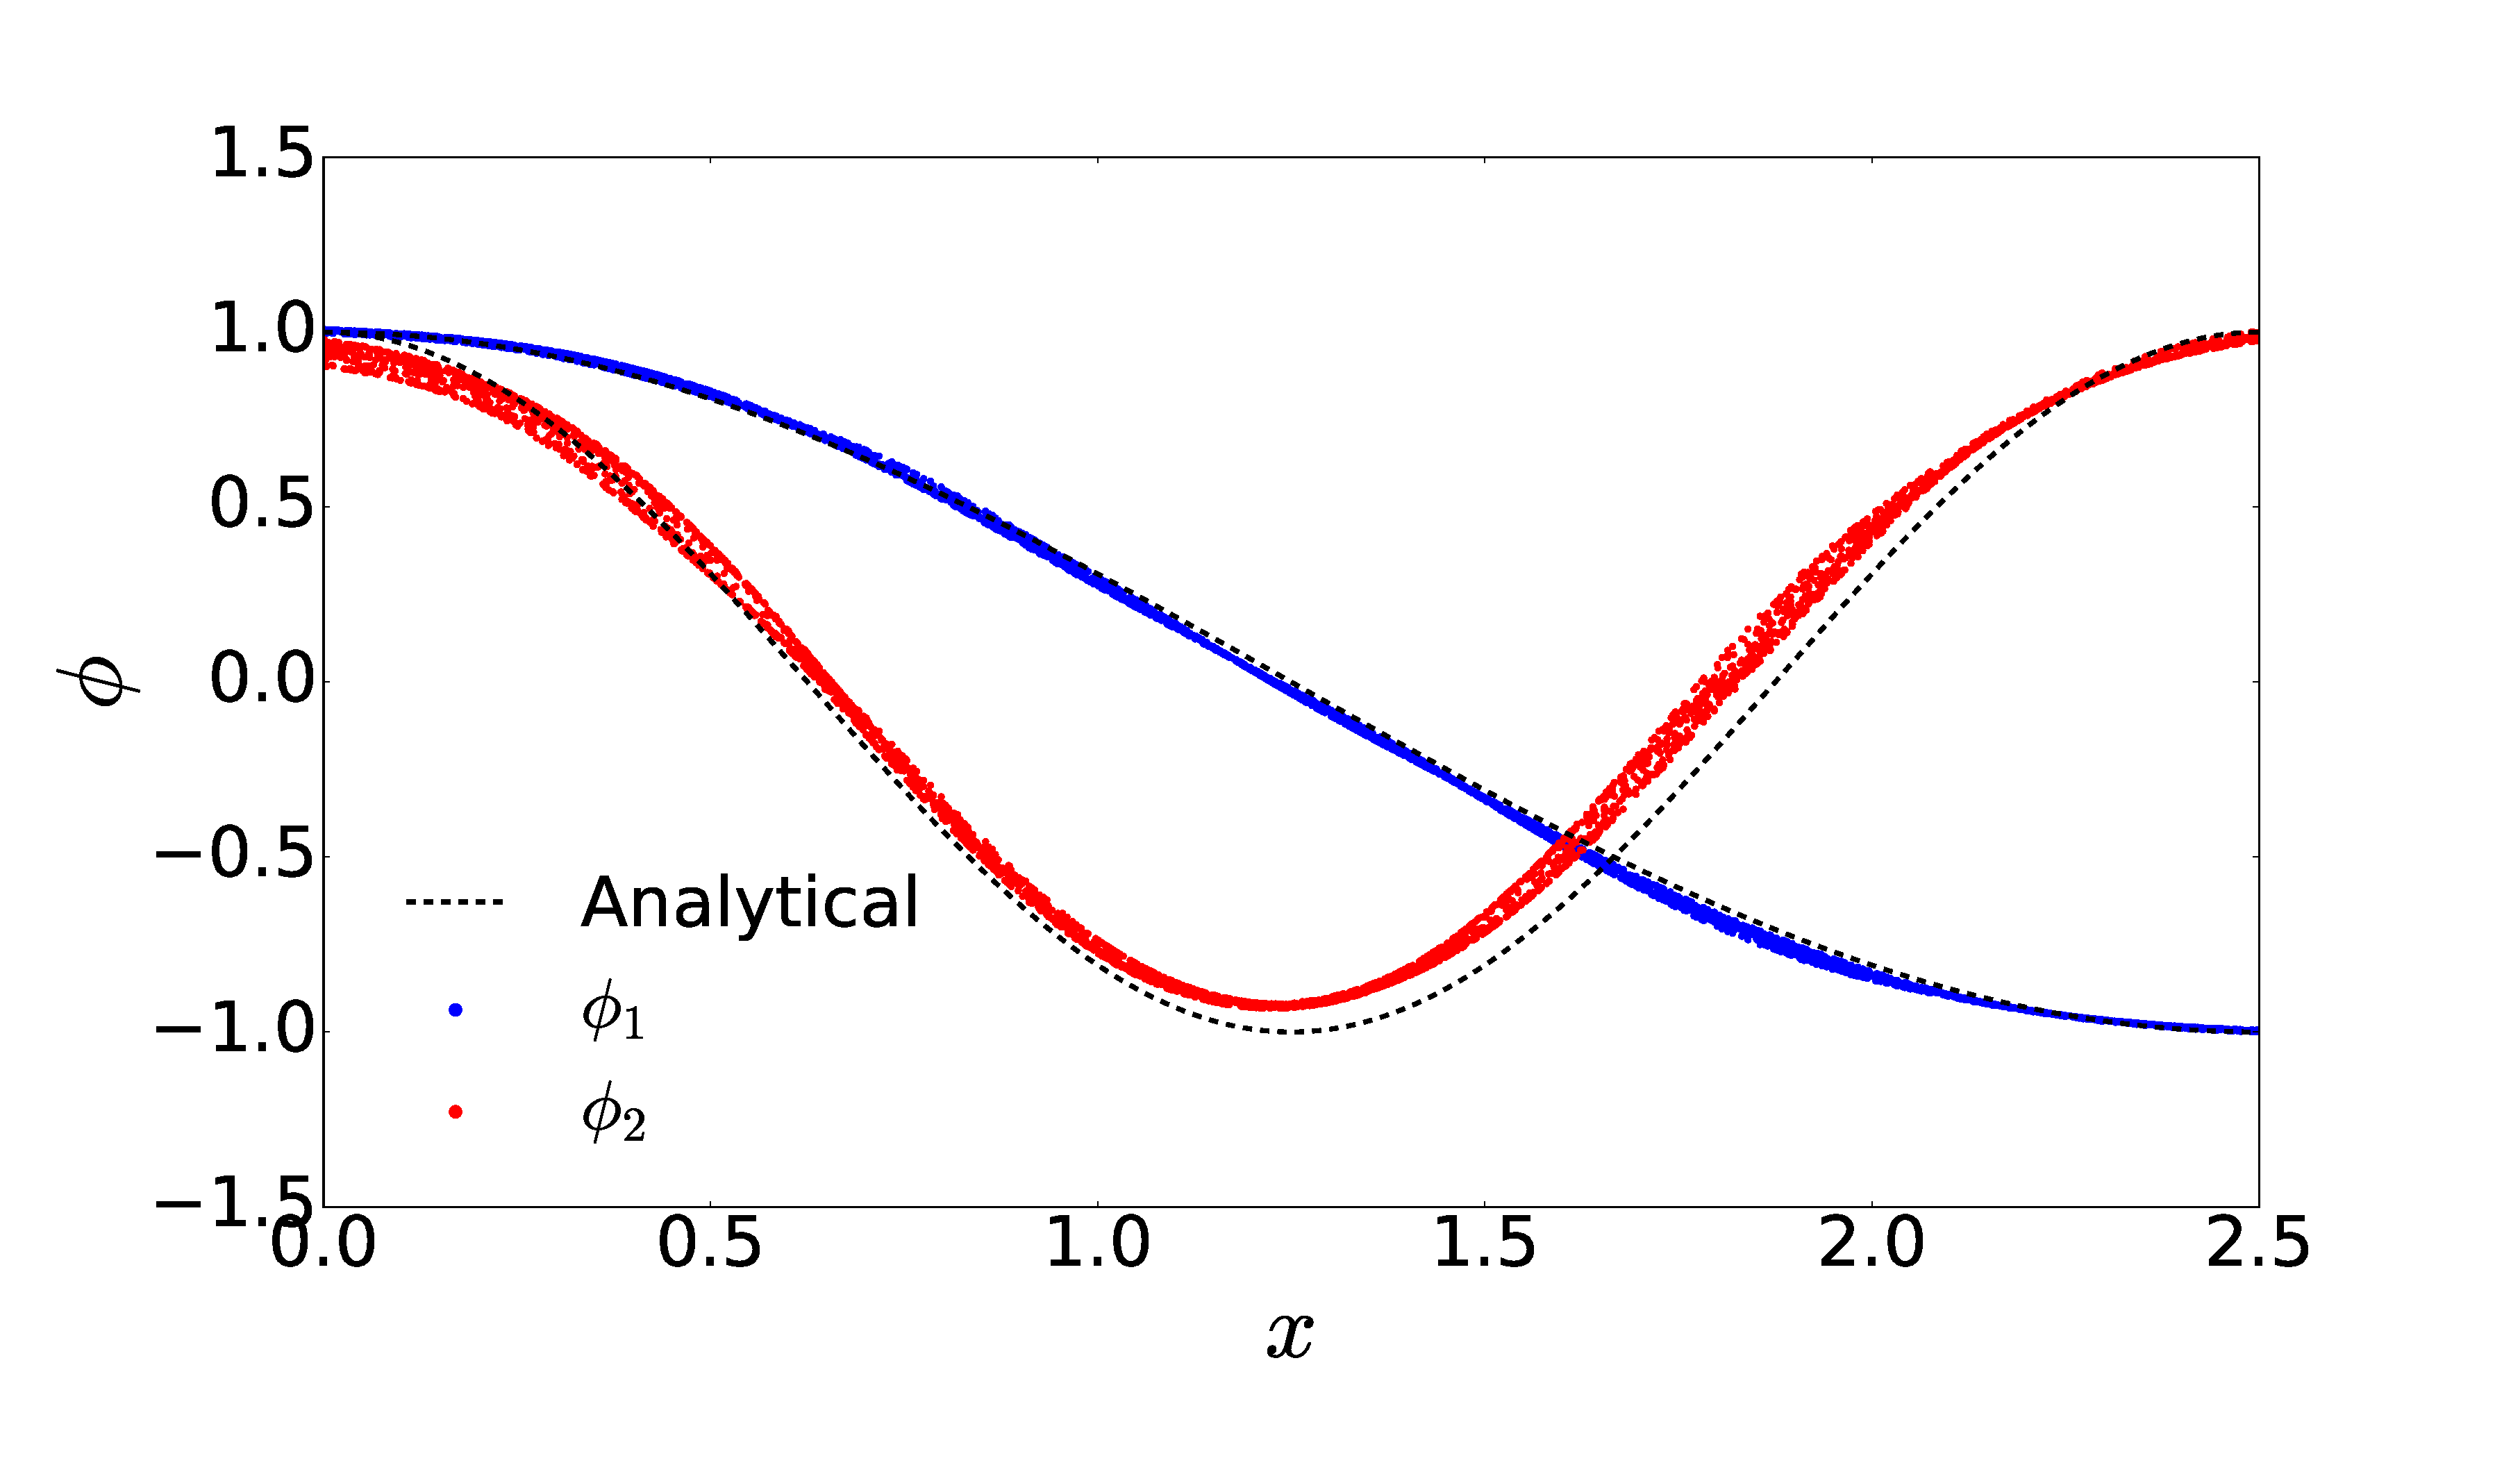
\includegraphics[width=\linewidth]{dmaps-comp-x}
    \subcaption{Comparison of numerical and analytical results for
      $\phi_1 \approx f_{10}$ and $\phi_2 \approx f_{20}$, both of
      which parameterize the $x$ direction.}
  \end{subfigure}
  % \hspace{0.5cm}
  \begin{subfigure}[t]{0.45\linewidth}
    \centering
    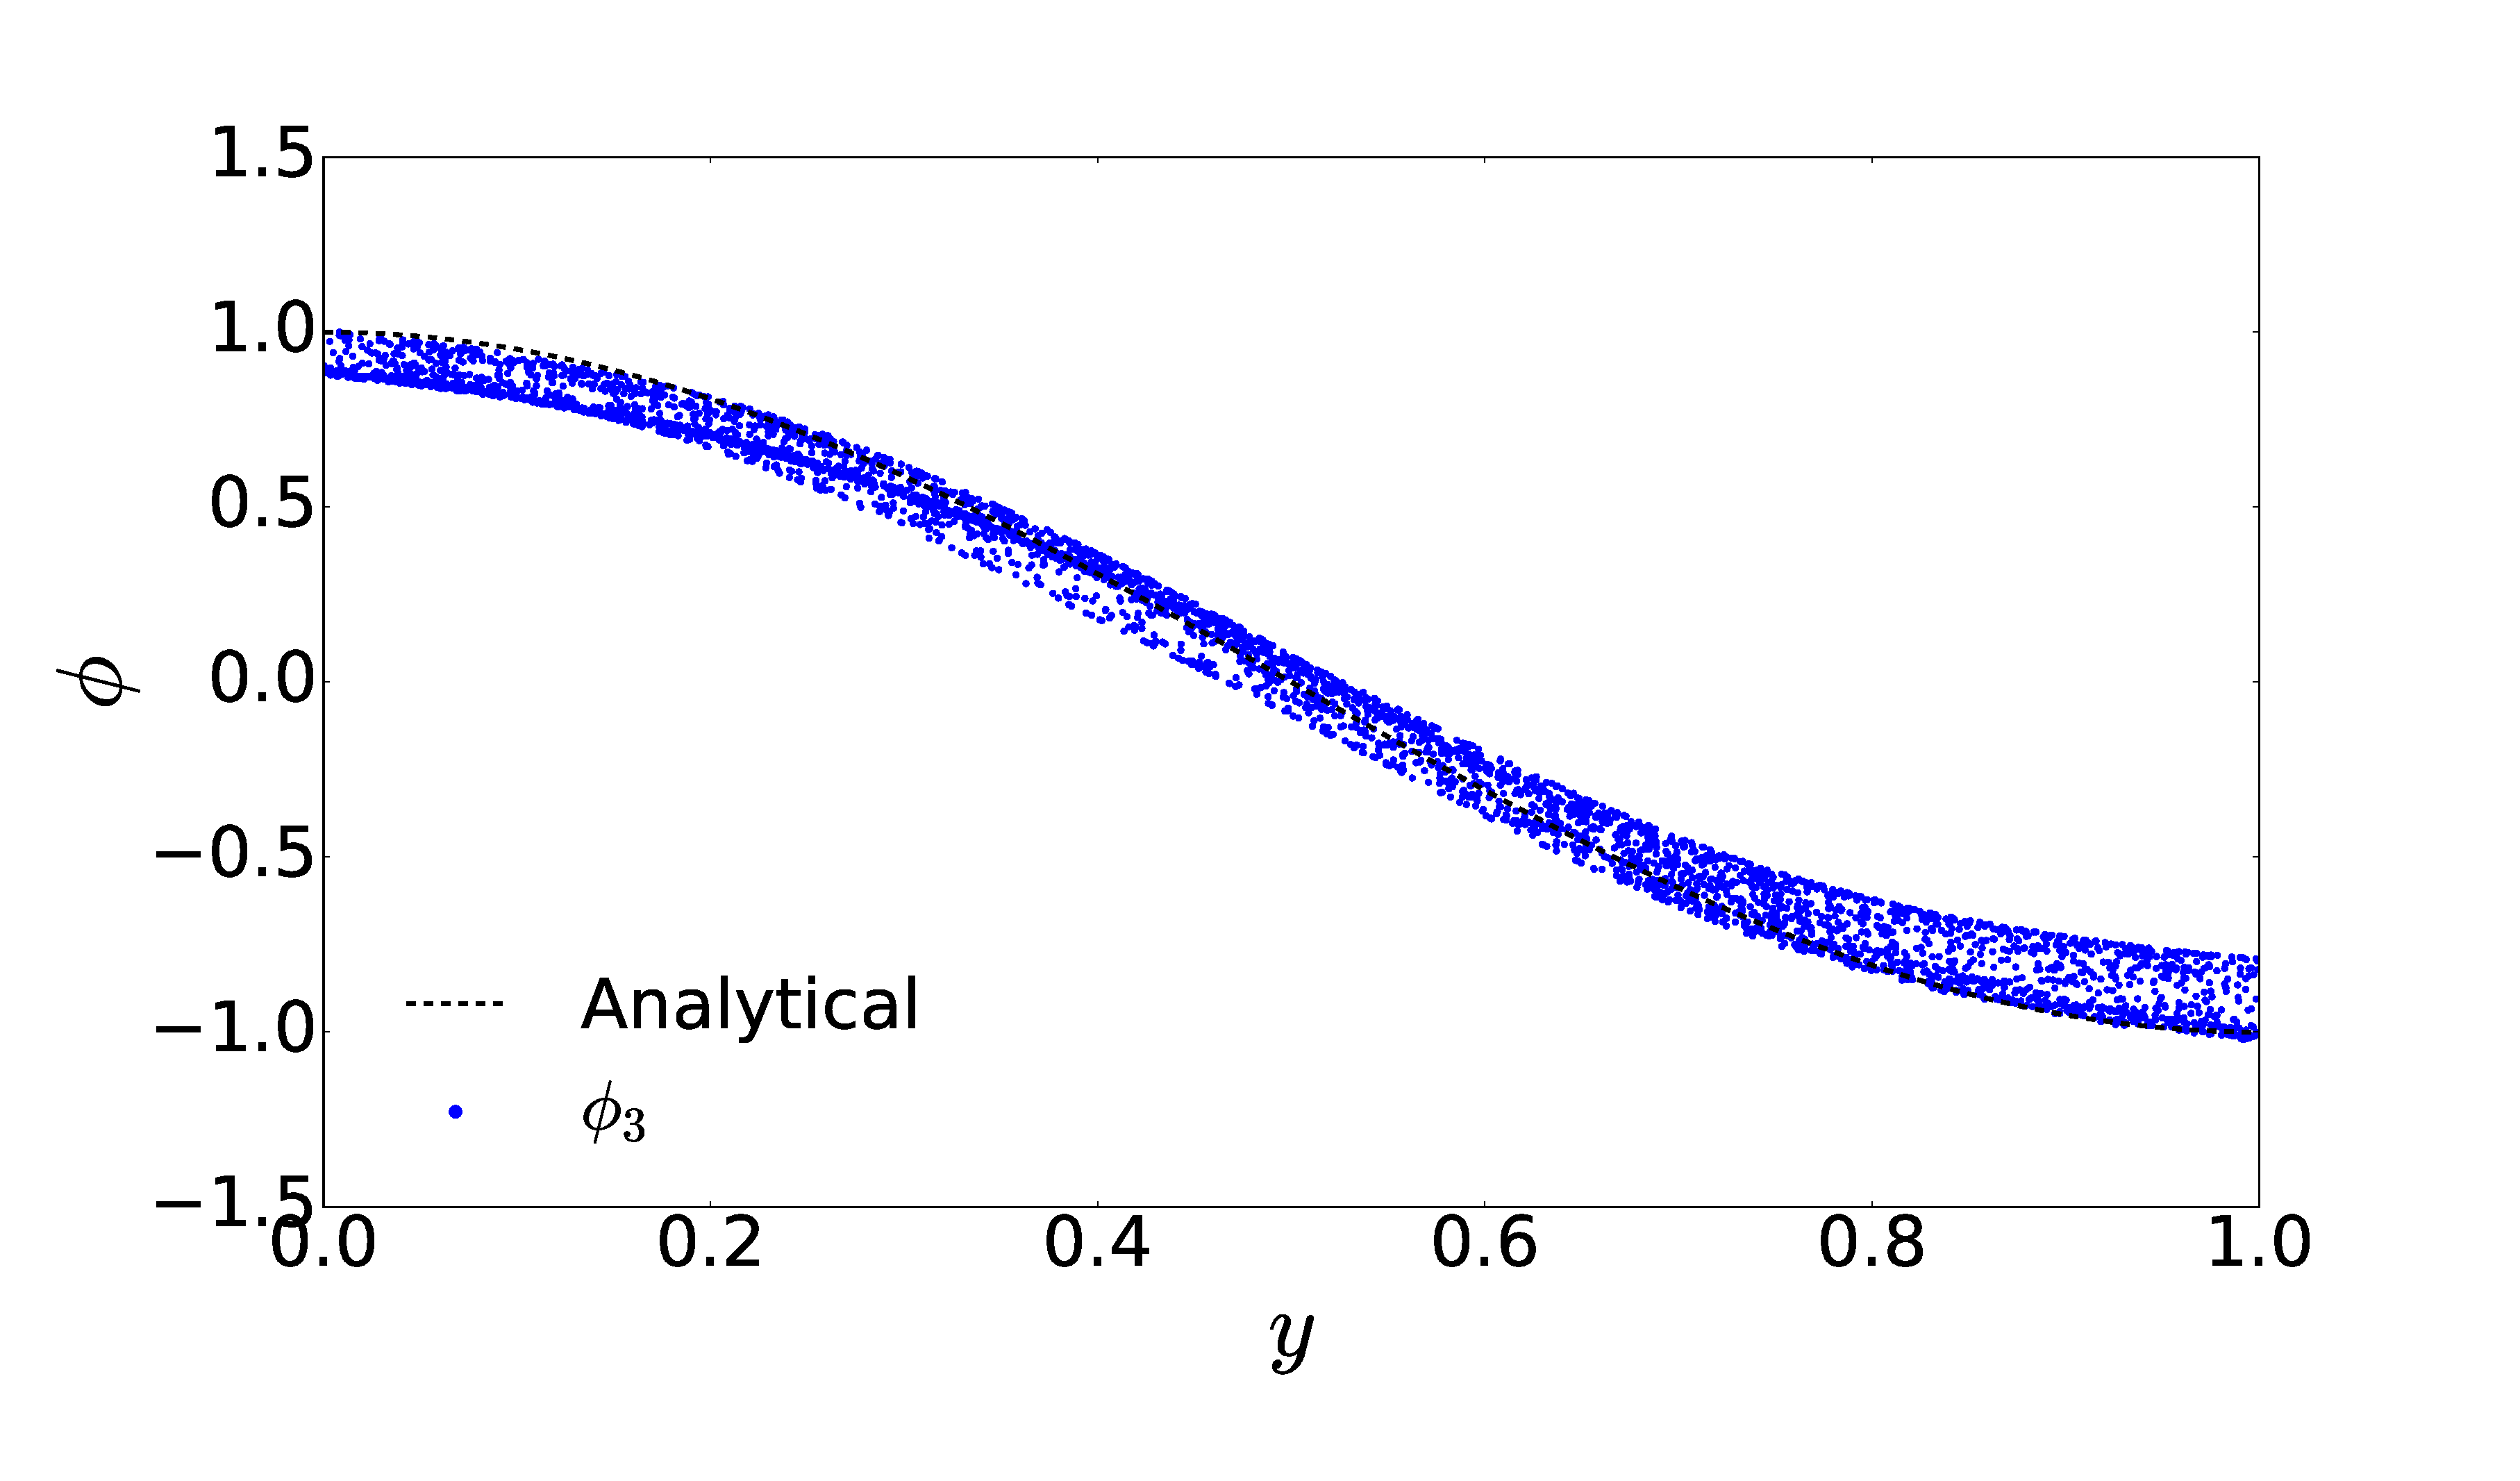
\includegraphics[width=\linewidth]{dmaps-comp-y}
    \subcaption{Comparison of numerical and analytical results for
      $\phi_3 \approx f_{01}$ which parameterizes the $y$ direction.}
  \end{subfigure}
  \caption[Example of DMAPS' parameterization of
  rectangle]{ \label{fig:dmaps-comp} }
\end{figure}

\begin{figure}
  \centering
  \begin{subfigure}[t]{0.45\linewidth}
    \centering
    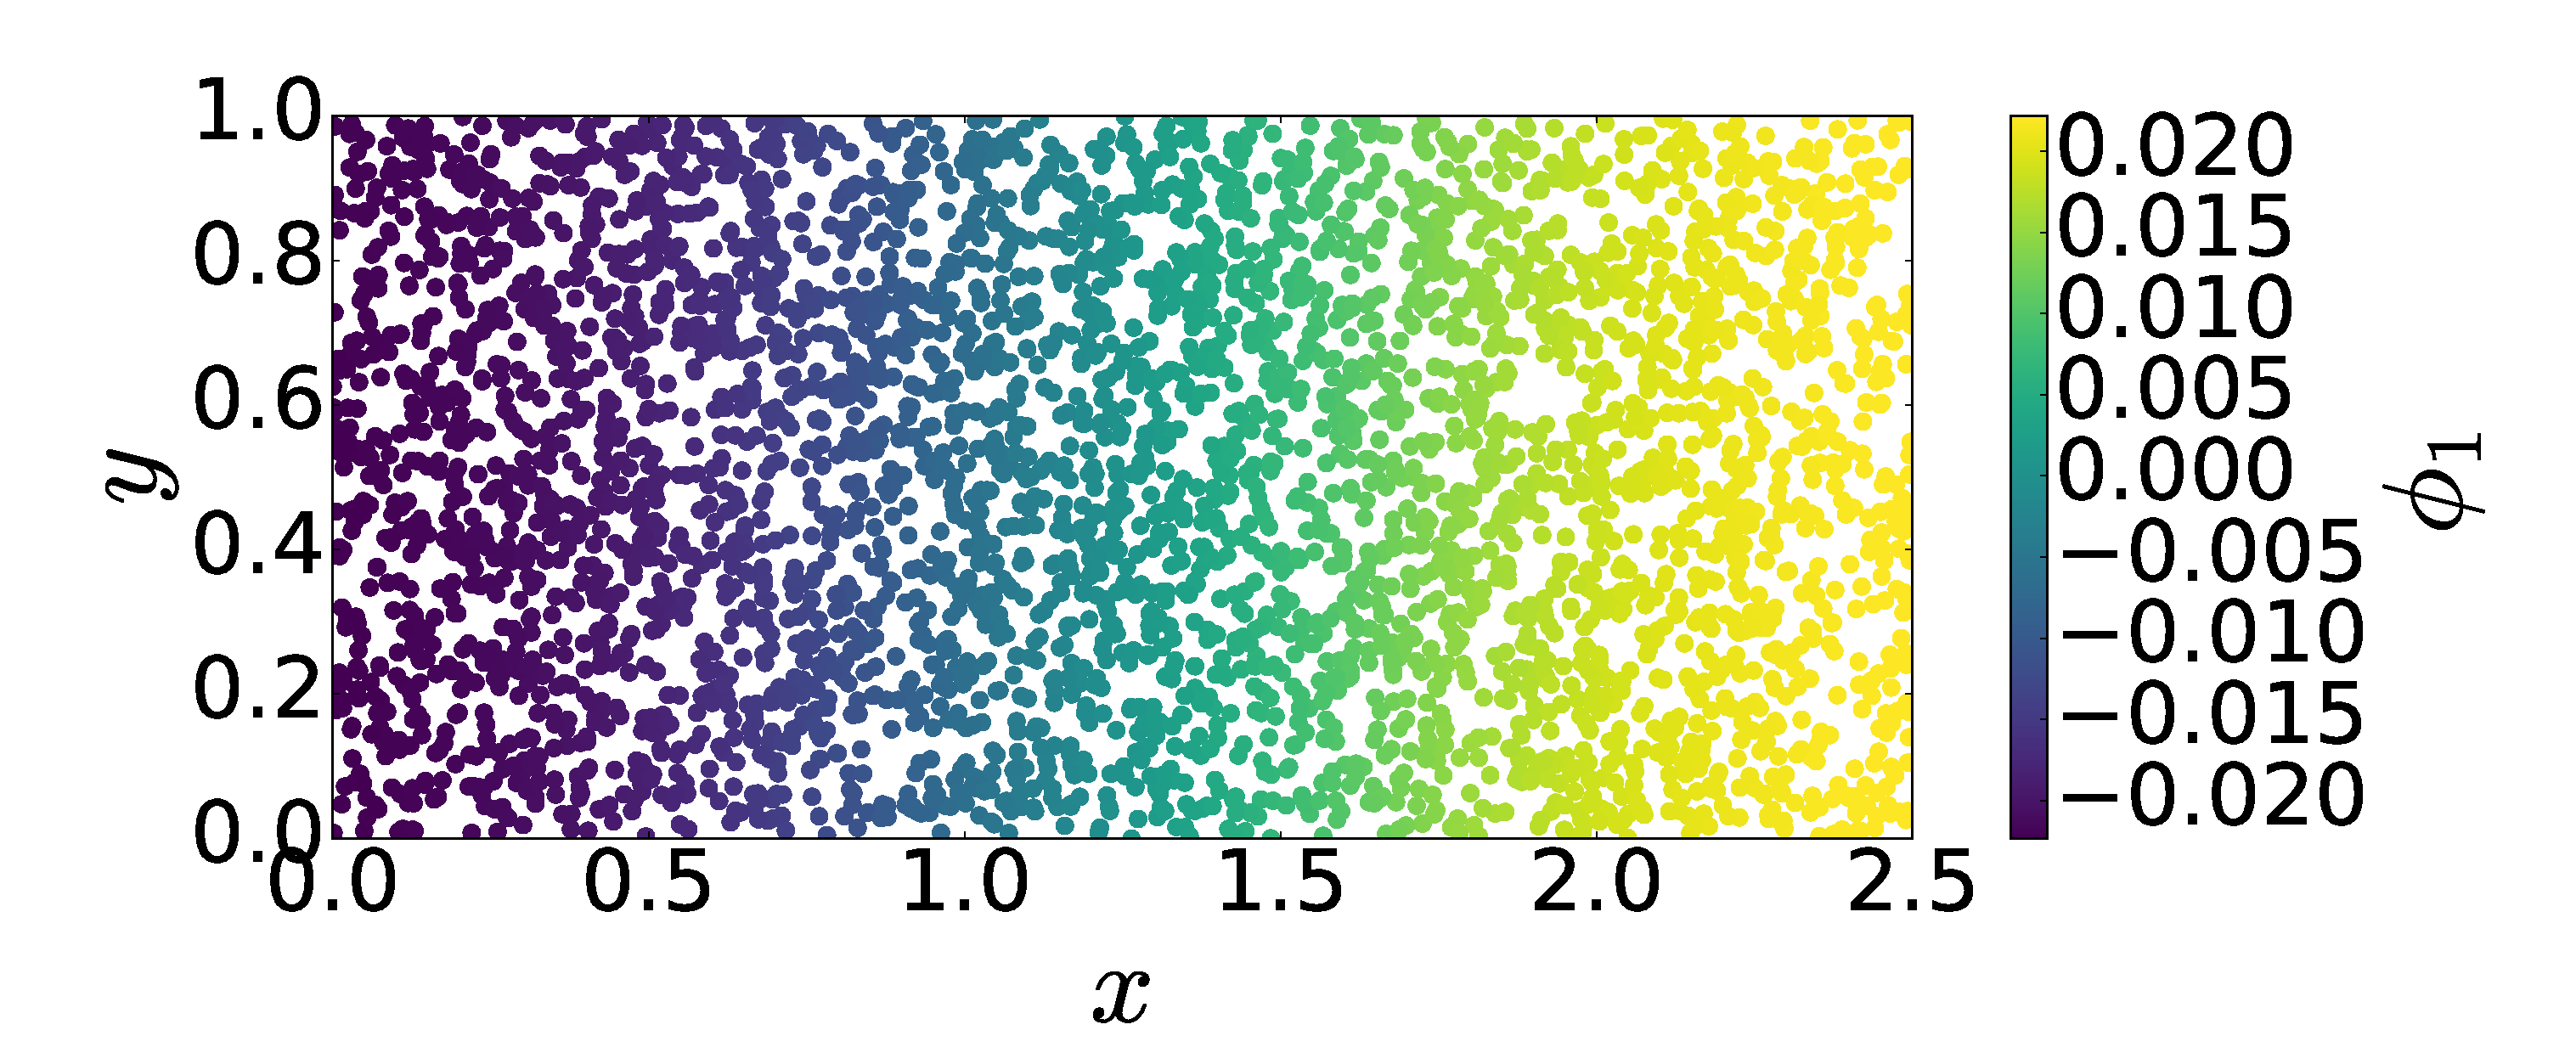
\includegraphics[width=\linewidth]{dmaps-x}
    \subcaption{Coloring the dataset by $\phi_1$, showing that
      $\phi_1$ changes in the $x$ direction.}
  \end{subfigure}
  % \hspace{0.5cm}
  \begin{subfigure}[t]{0.45\linewidth}
    \centering
    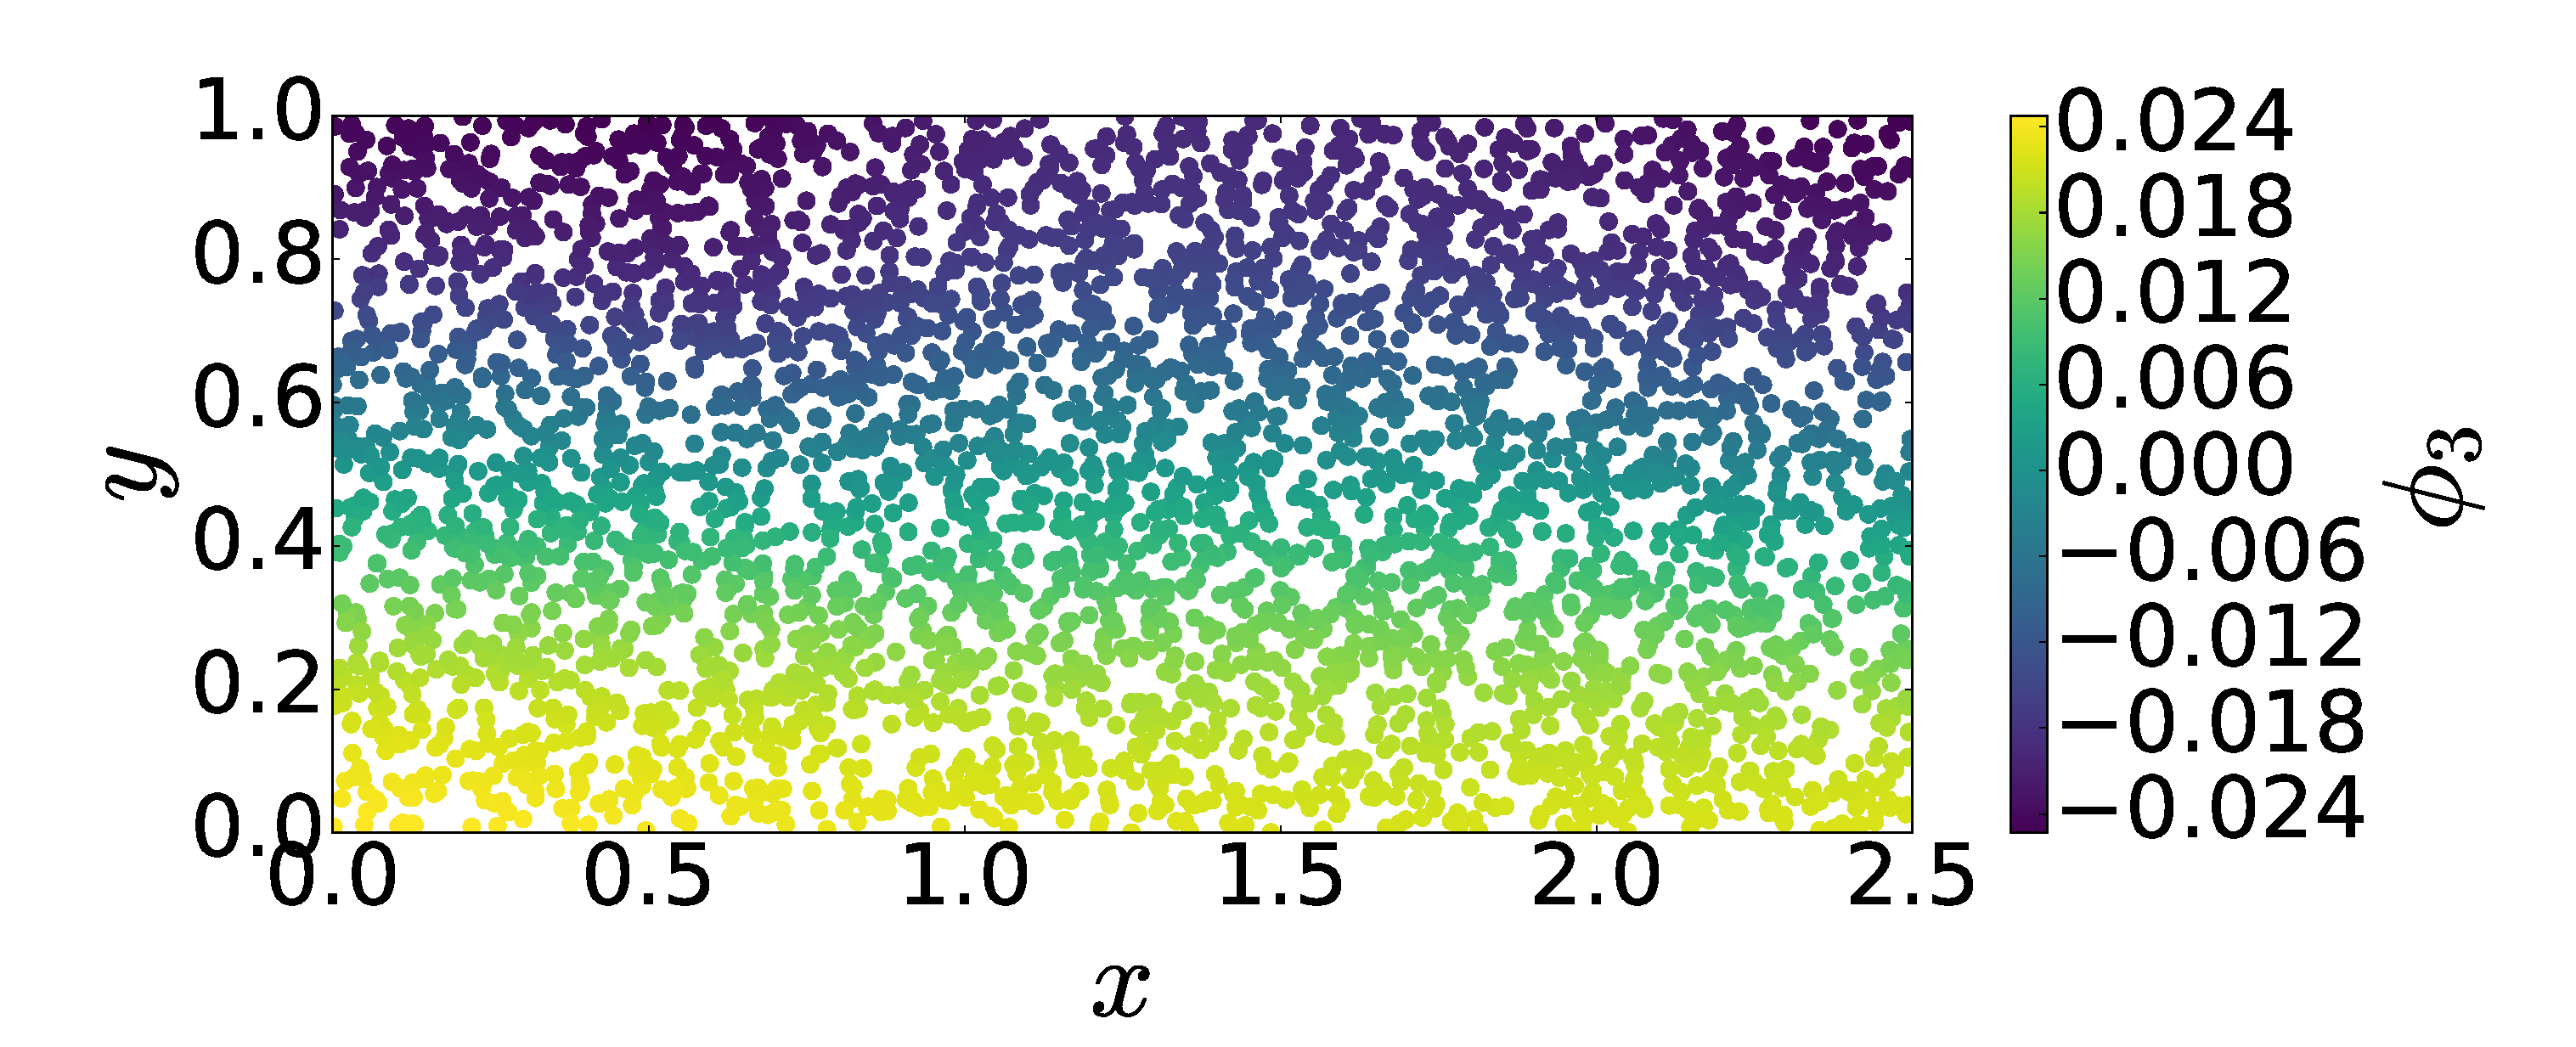
\includegraphics[width=\linewidth]{dmaps-y}
    \subcaption{Coloring the dataset by $\phi_3$, showing that
      $\phi_3$ changes in the $y$ direction.}
  \end{subfigure}
  \caption[Comparison of analytical and numerical DMAPS results]{ \label{fig:dmaps-xy} }
\end{figure}

However, if the density of our points is nonuniform over the rectangle
as shown in Fig.~\ref{fig:dmaps-nonun-data}, the output of algorithm
~\ref{alg:dmaps-unnorm} will be affected by the particular
distribution of points. On the other hand, ~\ref{alg:dmaps} will
continue to approximate eigenfunctions of $\nabla
f$. Fig.~\ref{fig:dmaps-nonun-phi} confirms this behavior.

\begin{figure}
    \centering
    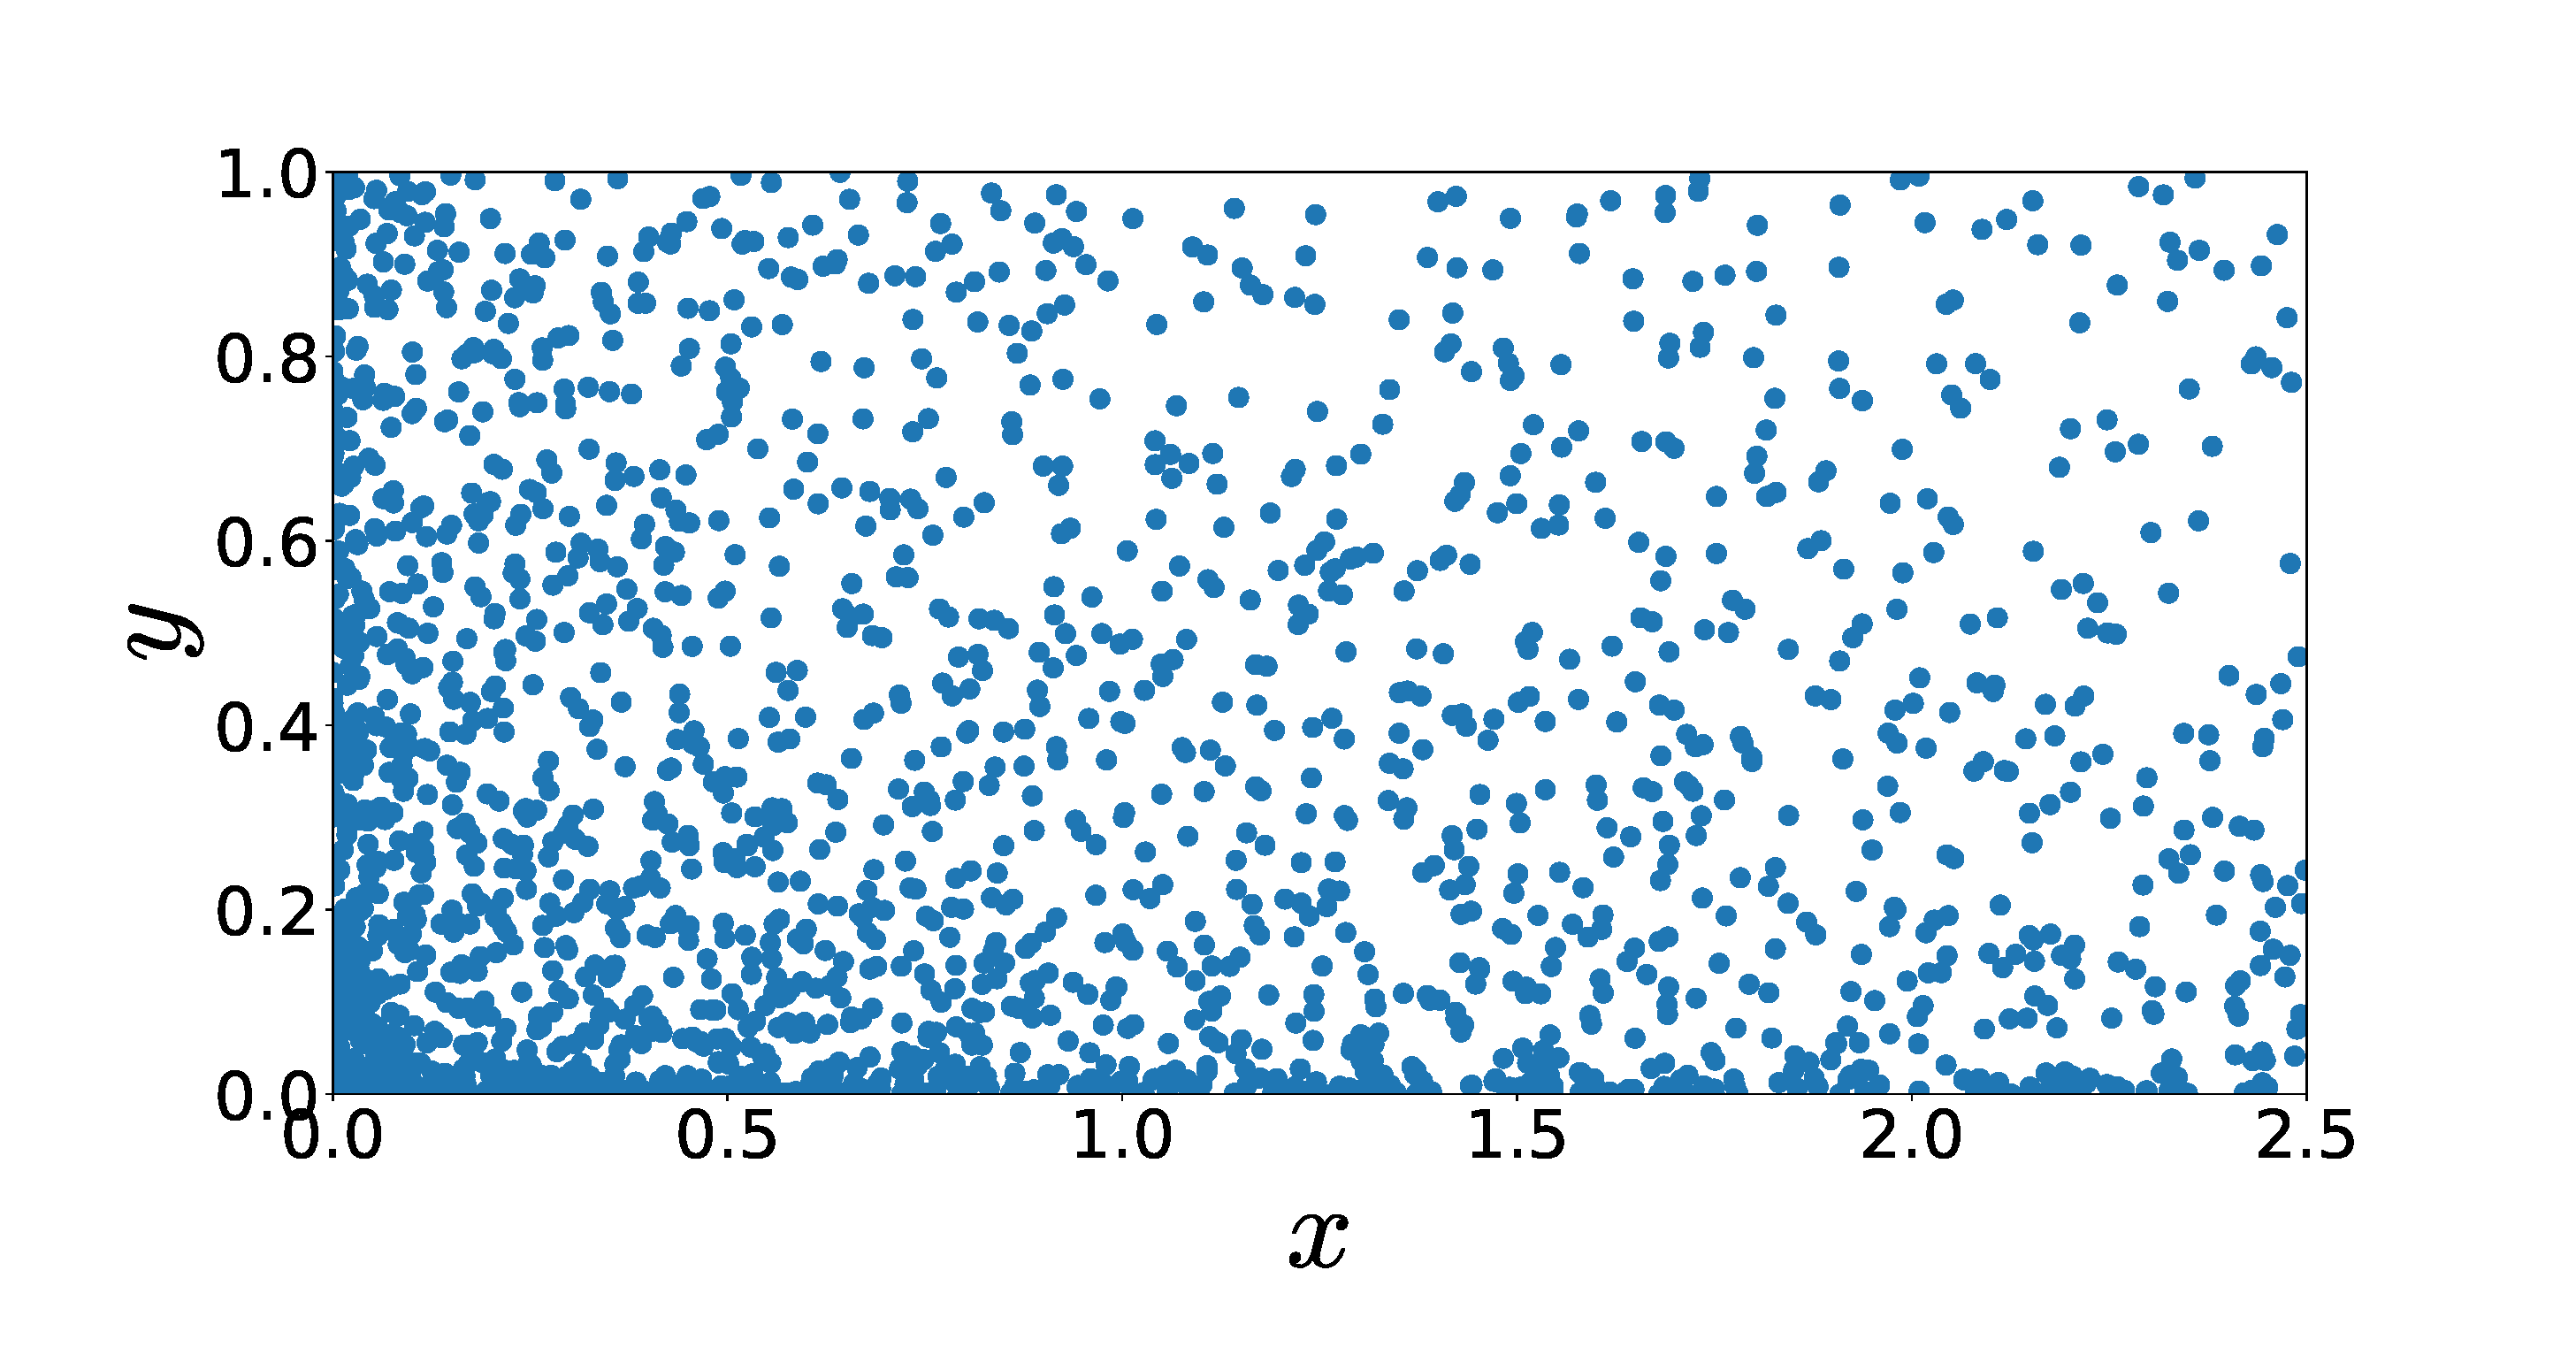
\includegraphics[width=0.9\linewidth]{data-non-y-x}
    \caption[Data with nonuniform density]{Data sampled nonuniformly over the
      rectangle. \label{fig:dmaps-nonun-data} }
\end{figure}


\begin{figure}
  \centering
  \begin{subfigure}[t]{0.45\linewidth}
    \centering
    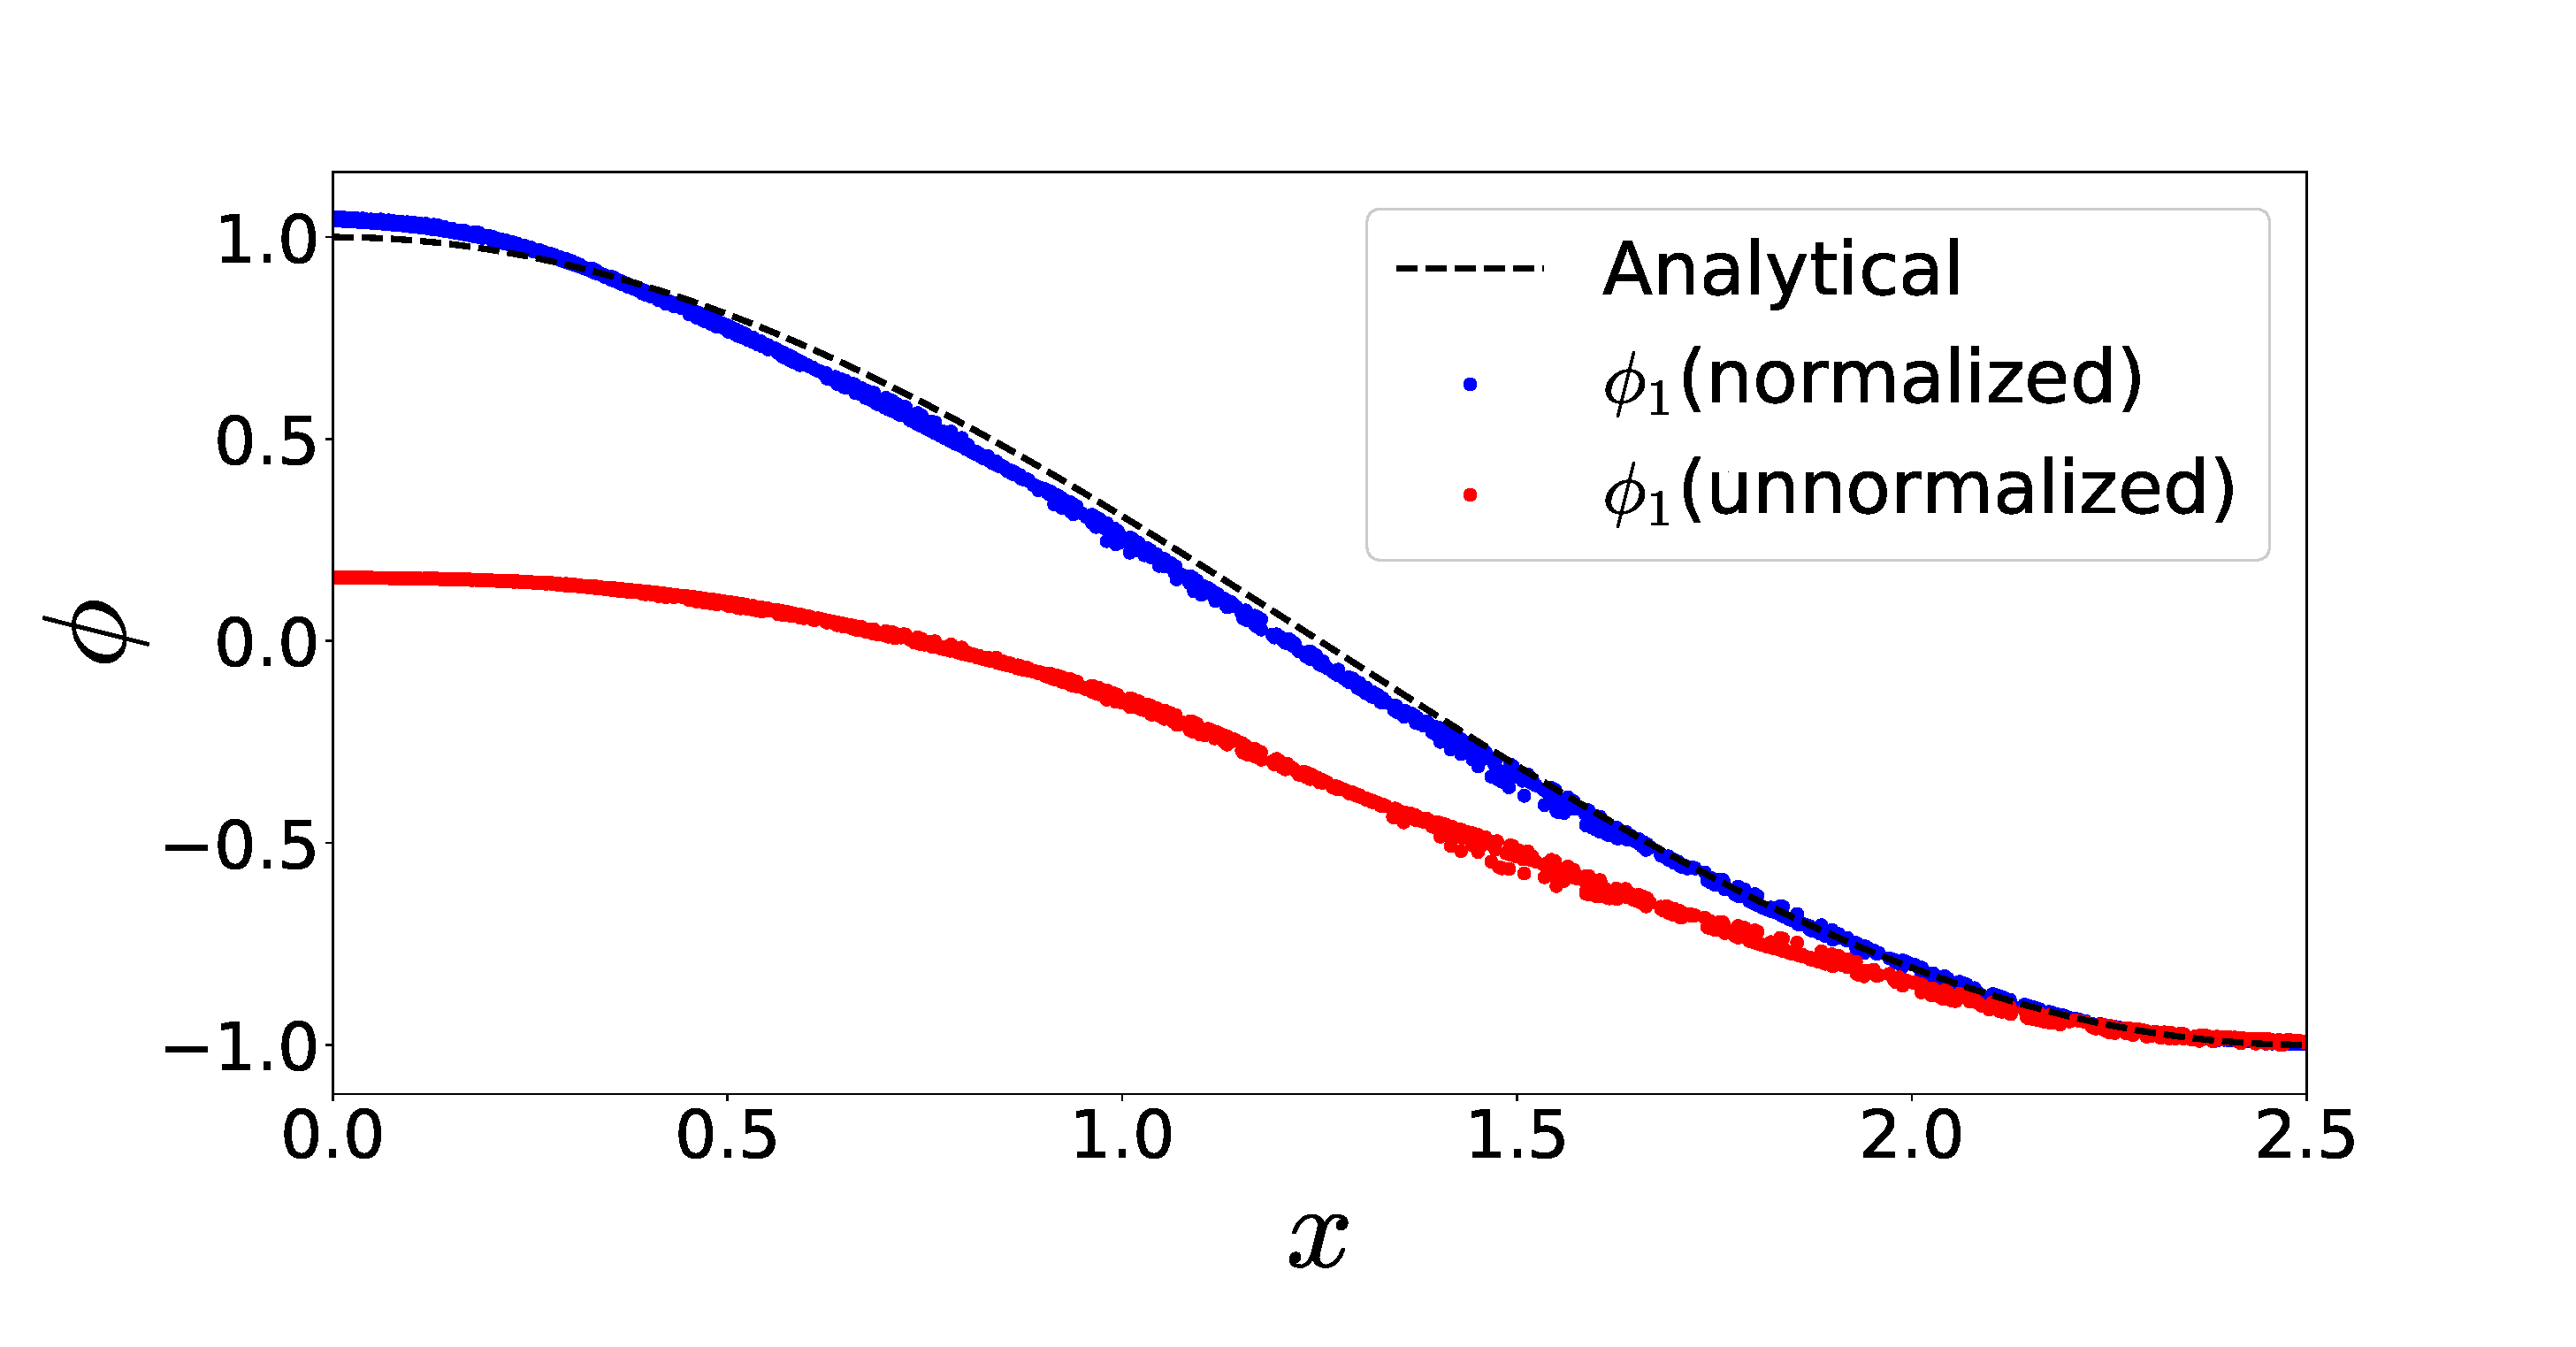
\includegraphics[width=\linewidth]{dmaps-non-x}
    \subcaption{Results for $\phi_1 \approx f_{10}$.}
  \end{subfigure}
  % \hspace{0.5cm}
  \begin{subfigure}[t]{0.45\linewidth}
    \centering
    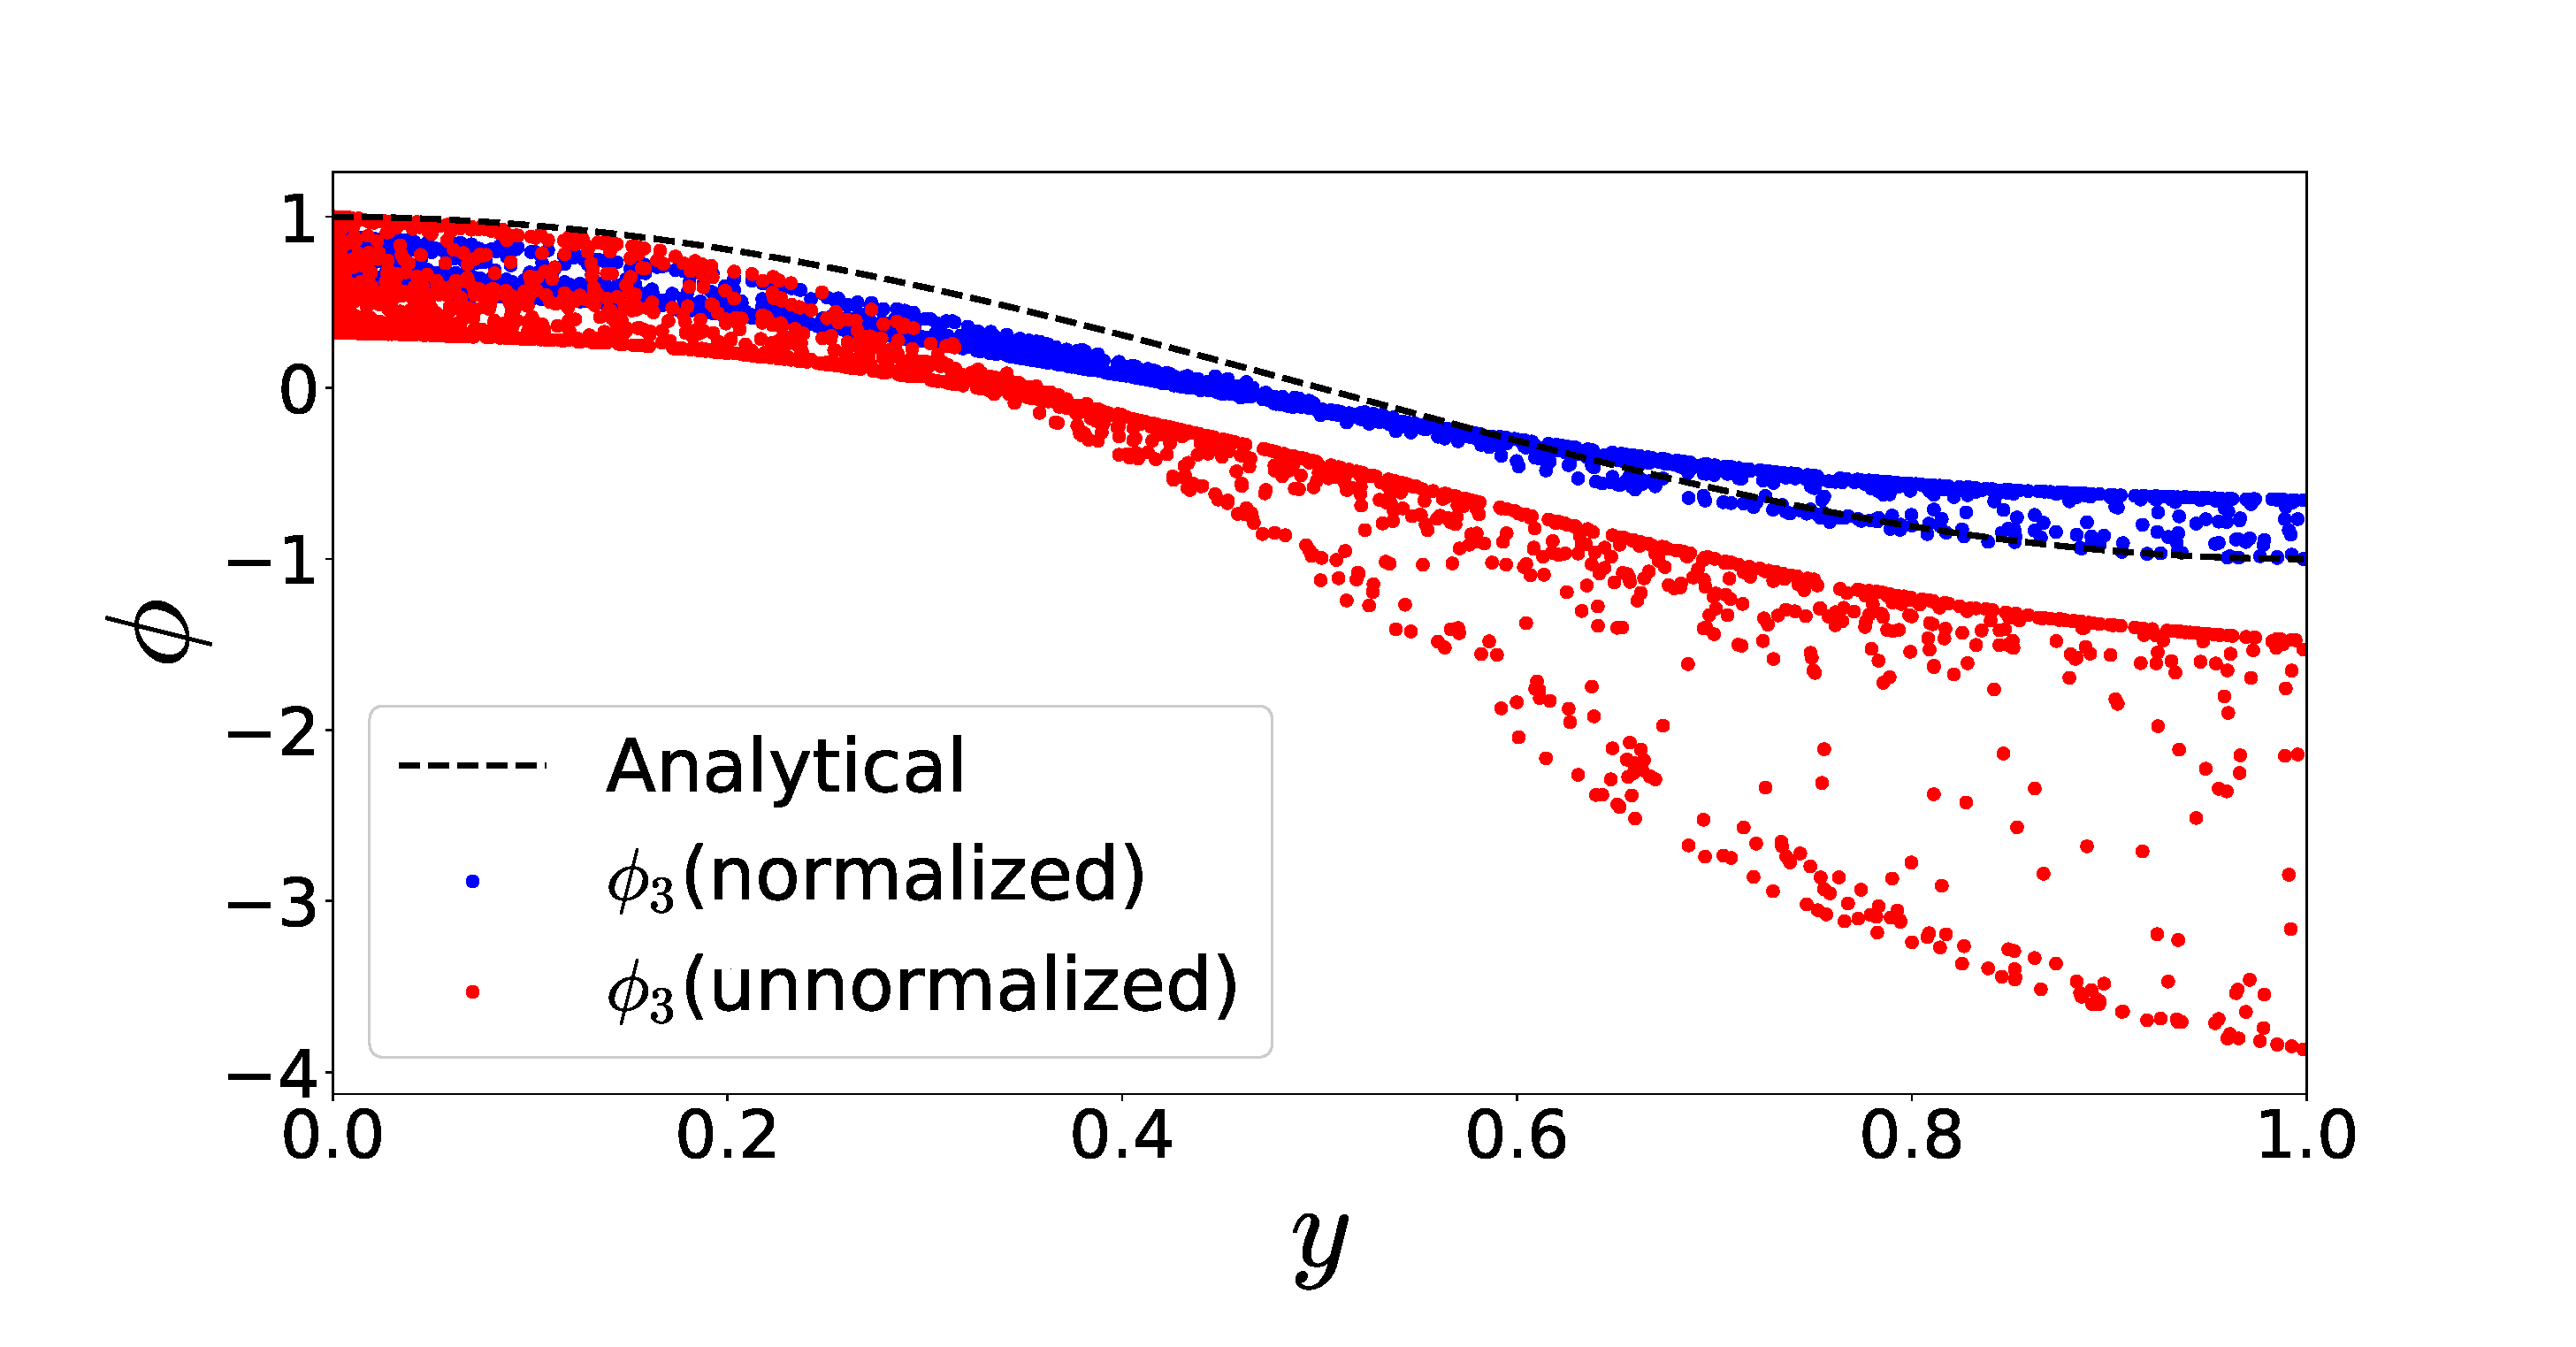
\includegraphics[width=\linewidth]{dmaps-non-y}
    \subcaption{Results for $\phi_3 \approx f_{01}$.}
  \end{subfigure}
  \caption[Comparison of different DMAPS variants]{Comparison of analytical result with normalized and
    unnormalized DMAPS variants showing that the normalized version
    captures the eigenfunctions of the Laplace operator regardless the
    point distribution. \label{fig:dmaps-nonun-phi} }
\end{figure}

The great benefit of DMAPS over PCA is its ability to parameterize
nonlinear manifolds. This comes at the cost of interpretability, as we
now lack an explicit connection between the input, $X$, and the output
$\phi_i$. In certain numerical applications this understanding is
unimportant. When one is interested in an intuitive physical
interpretation of the low-dimensional description, the DMAPS output
can be used to test hypotheses about which variable combinations are
significant.

%%% Local Variables: ***
%%% mode:latex ***
%%% TeX-master: "../../thesis.tex"  ***
%%% End: ***
\section{Equation-free modeling\label{sec:ef}}

The second key component in the work that follows is Equation Free
(EF) modeling. This framework enables one to analyze agent-based
simulations such as social network evolution or molecular dynamics
using systems-level algorithms without deriving explicit, analytical
equations governing the properties of interest
\cite{gear_equation-free_2003,kevrekidis_equation-free:_2004}. EF
modeling has been used to accelerate simulations, to locate coarse
steady states, and to perform bifurcation analysis, using only the
sort of fine-scale simulations that researchers across disciplines
increasingly rely on to model their
problems~\cite{tsoumanis_coarse-graining_2012,ferguson_systematic_2010,bold_equation-free_2014}. We
will now provide an overview of the general framework, and a
particular application known as coarse projective integration.

EF techniques rely on two complementary algorithmic elements: a
restriction operator $\Res$ that maps fine-scale simulations to coarse
variables, and a lifting operator $\Li$ that maps coarse variables to
consistent fine-scale simulations. Thus lifting is the inverse of
restriction, so $\Res \cdot \Li (x) = x$. We will denote the state of
the fine system by $u(t)$, with $U(t)$ the corresponding coarse
state. $u(t)$ could represent the evolving state of neurons in a
simulation of brain activity, while $U(t)$ may track the average
action potential. In such complex models it is difficult to derive an
explicit formula governing the progression of $U(t)$, but by
periodically measuring this quantity as the simulation progresses,
through $\Res: u \rightarrow U$, we can estimate its trajectory. Then,
using an integration scheme as simple as forward Euler, we may
approximate the value of $U(t)$ at some future time,
$U(t + \Delta t)$. Using $\Li: U \rightarrow u$ we obtain a fine-scale
state $u(t + \Delta t)$. This process of alternately restricting and
lifting can be repeated until the system has reached a desired
state. Overall, the result is an accelerated simulation as we have
replaced $\Delta t$ expensive, full-system steps with a single, cheap
application of forward Euler during each iteration. This method is
known as coarse projective integration (CPI), and it is illustrated in
Fig.~\ref{fig:cpi-ill}. This forms the backbone of EF modeling, and in
Chapter~\ref{ch:graphs} we will see how CPI can be used to implement a
stationary-state solver for evolving networks.

\begin{figure}
  \centering
  \includegraphics[width=0.8\textwidth]{cpi-intro}
  \caption[Illustration of coarse projective integration]{Illustration
    of CPI procedure in which repeated applications of the restriction
    operator $\Res$ are used to approximate the trajectory of $U(t)$
    and to estimate its value at some future time $U(t + \Delta
    t)$. Subsequent application of $\Li$ allows one to iterate this
    process, accelerating simulations. \label{fig:cpi-ill}}
\end{figure}

%%% Local Variables: ***
%%% mode:latex ***
%%% TeX-master: "../../thesis.tex"  ***
%%% End: ***

%%% Local Variables: ***
%%% mode:latex ***
%%% TeX-master: "../../thesis.tex"  ***
%%% End: ***
% !TEX root = ../thesis.tex

\chapter{Reduced descriptions of collections of
  networks \label{ch:graphs}}

% \abstract{In order to illustrate the adaptation of traditional
% continuum numerical techniques to the study of complex network
% systems, we use the equation-free framework to analyze a dynamically
% evolving multigraph.
% %
% This approach is based on coupling short intervals of direct dynamic
% network simulation with appropriately-defined lifting and
% restriction operators, mapping the detailed network description to
% suitable macroscopic (coarse-grained) variables and back.
% %
% This enables the acceleration of direct simulations through Coarse
% Projective Integration (CPI), as well as the identification of
% coarse stationary states via a Newton-GMRES method.
% %
% We also demonstrate the use of data-mining, both linear (principal
% component analysis, PCA) and nonlinear (diffusion maps, DMAPS) to
% determine good macroscopic variables (observables) through which one
% can coarse-grain the model.
% %
% These results suggest methods for decreasing simulation times of
% dynamic real-world systems such as epidemiological network
% models. Additionally, the data-mining techniques could be applied to
% a diverse class of problems to search for a succint, low-dimensional
% description of the system in a small number of variables.}


\section{Introduction\label{sec:intro}}
  

Over the past decades, complex networks have been used as the model of
choice for a truly broad class of physical problems, ranging from
highway traffic \cite{joubert_large-scale_2010} to brain connectivity
\cite{hermundstad_learning_2011}.
%
When modeling such systems, dynamics are typically defined at a very
detailed, ``fine'' scale, specifying individual node and edge
interactions; explicit closed equations governing network macroscopic
(collective) properties are often unavailable
\cite{durrett_graph_2012,joubert_large-scale_2010,roche_agent-based_2011,swaminathan_modeling_1998}.
%
The detailed interactions are often complicated functions dependent on
multiple system parameters, which, when one also accounts for large
network sizes inherent in many interesting problems, can make
systematic numerical exploration computationally prohibitive.
%
The lack of \textit{explicit} macroscopic equations prohibits the use
of traditional numerical techniques such as fixed-point computation
and stability analysis, that could offer valuable insight into the
network's behavior, leaving little alternative but to work with full
direct simulations of the entire network.
%
Faced with these inherent limitations, investigators must either
restrict their attention to a more modest parameter space
\cite{hodgkin_quantitative_1952} or simplify the network model,
potentially removing important features
\cite{brown_variability_1999}. \par

Equation-free modeling offers a promise to circumvent these
challenges, allowing one to investigate the complex network at a
macroscopic level while retaining the effects of full system details
\cite{kevrekidis_equation-free:_2004,gear_equation-free_2003}.
%
Underlying this method is the assumption that, although we cannot
analytically derive equations governing network evolution, such closed
equations do, in principle, exist.
%
Furthermore, these unavailable equations are assumed to involve a
small number of dominant collective (coarse-grained) variables.
%
The important features of the complete network can be in fact, by this
assumption, well represented by these select observable quantities.
%
This may seem too restrictive, yet it is exactly the behavior
witnessed across many network types: despite the initial complexity of
the full system configuration, certain collective network properties
appear to evolve smoothly in time, while the evolution of other,
``secondary'' properties, can be strongly correlated with that of the
few ``primary'' variables
\cite{bold_equation-free_2014,rajendran_coarse_2011,siettos_equation-free_2011}.
%
Once these significant variables are uncovered, we can combine short
intervals of full system simulation with operators that map the full
system description to and from its representative coarse variable
``summary'', thus enabling previously-infeasible system-level analysis
(see Section \ref{sec:ef} for further details). \par

Here, we apply this framework to a dynamically evolving multigraph
model.
%
This offers a test of the methodology in the previously unexplored
context of multigraphs.
%
We demonstrate the acceleration of direct network simulations through
Coarse Projective Integration (CPI), and the location of coarse
stationary states through a matrix-free Newton-GMRES method.
%
In addition, principal component analysis (PCA) and diffusion maps
(DMAPS), two well established dimensionality-reduction techniques, are
shown to enable an algorithm for characterization of the underlying
low-dimensional behavior of the system. \par

The paper is organized as follows: we begin in Section \ref{sec:m}
with a description of the multigraph dynamic model.
%
Sections \ref{sec:ef} and \ref{sec:ng} provide most details of the
equation-free approach, specify how it was applied to our system, and
present subsequent results.
%
Section \ref{sec:dr} summarizes our use of PCA and DMAPS, and assesses
their effectiveness in analyzing hidden, low-dimensional structure in
this network system.

\section{Model description\label{sec:m}}

We study the edge-conservative preferential attachment model, a
detailed mathematical analysis of which can be found in
\cite{rath_time_2012} and \cite{rath_multigraph_2012}.
%
The system evolves in discrete steps $t = 0,1,\ldots t_f$, and we
denote the $n$-vertex graph at each point by $G_n(t)$.
%
The initial state, $G_n(0)$, is an arbitrary distribution of $m$ edges
among the $n$ vertices; the total number of both edges and vertices is
conserved.
%
No restrictions are placed on this initial distribution: multiple
edges and loops are permitted.  The system is then advanced
step-by-step based on the following procedure:

\begin{enumerate}
\item Choose an edge $e_{ij} \in E(G)$ uniformly at random, and flip a
  coin to label one of the ends as $v_{i}$
\item Choose a vertex $v_{k}$ using linear preferential attachment:
  $P(v_{k} = v_{l}) = \frac{d_{l} + \kappa}{\sum\limits_{i=1}^{n}
    d_{i} + n \kappa}$
  \label{step:prob}
\item Replace $e_{ij}$ with $e_{ik}$,
\end{enumerate}

\noindent where $d_i$ is the degree of vertex $v_i$, $E(G)$ is the set
of edges in the graph, and $\kappa \in (0, \infty)$ is a model
parameter affecting the influence degrees have on the probability
distribution in Step \ref{step:prob}.
%
That is, taking $\lim\limits{\kappa \rightarrow 0}$, we recover
``pure'' preferential attachment, and probability scales directly with
degree, while
$\lim\limits_{\kappa \rightarrow \infty} P(v_k = v_l) = \frac{1}{n} \;
\forall \; l$, and individual degrees have no effect. A single step of
this evolution process is illustrated in
Fig. ({\ref{fig:step-illustration}}). Note that this can also be
represented as a graph in which only one edge is permitted between
each pair of nodes, but with edge weights signifying the number, or
strength, of connections between nodes.
\par

Evolving the system in this manner, the degree sequence approaches a
stationary distribution over $O(n^3)$ steps.
%
As explained in \cite{rath_time_2012}, this distribution is dependent
only on the system parameters $\rho = \frac{2*m}{n}$ and $\kappa$.
%
Fig. (\ref{fig:dse}) illustrates the evolution of the degree sequence
of two networks with different initial configurations but the same
values of $\rho$ and $\kappa$ respectively; as expected, we observe
they approach an identical stationary state.

  \begin{figure}
    \centering
    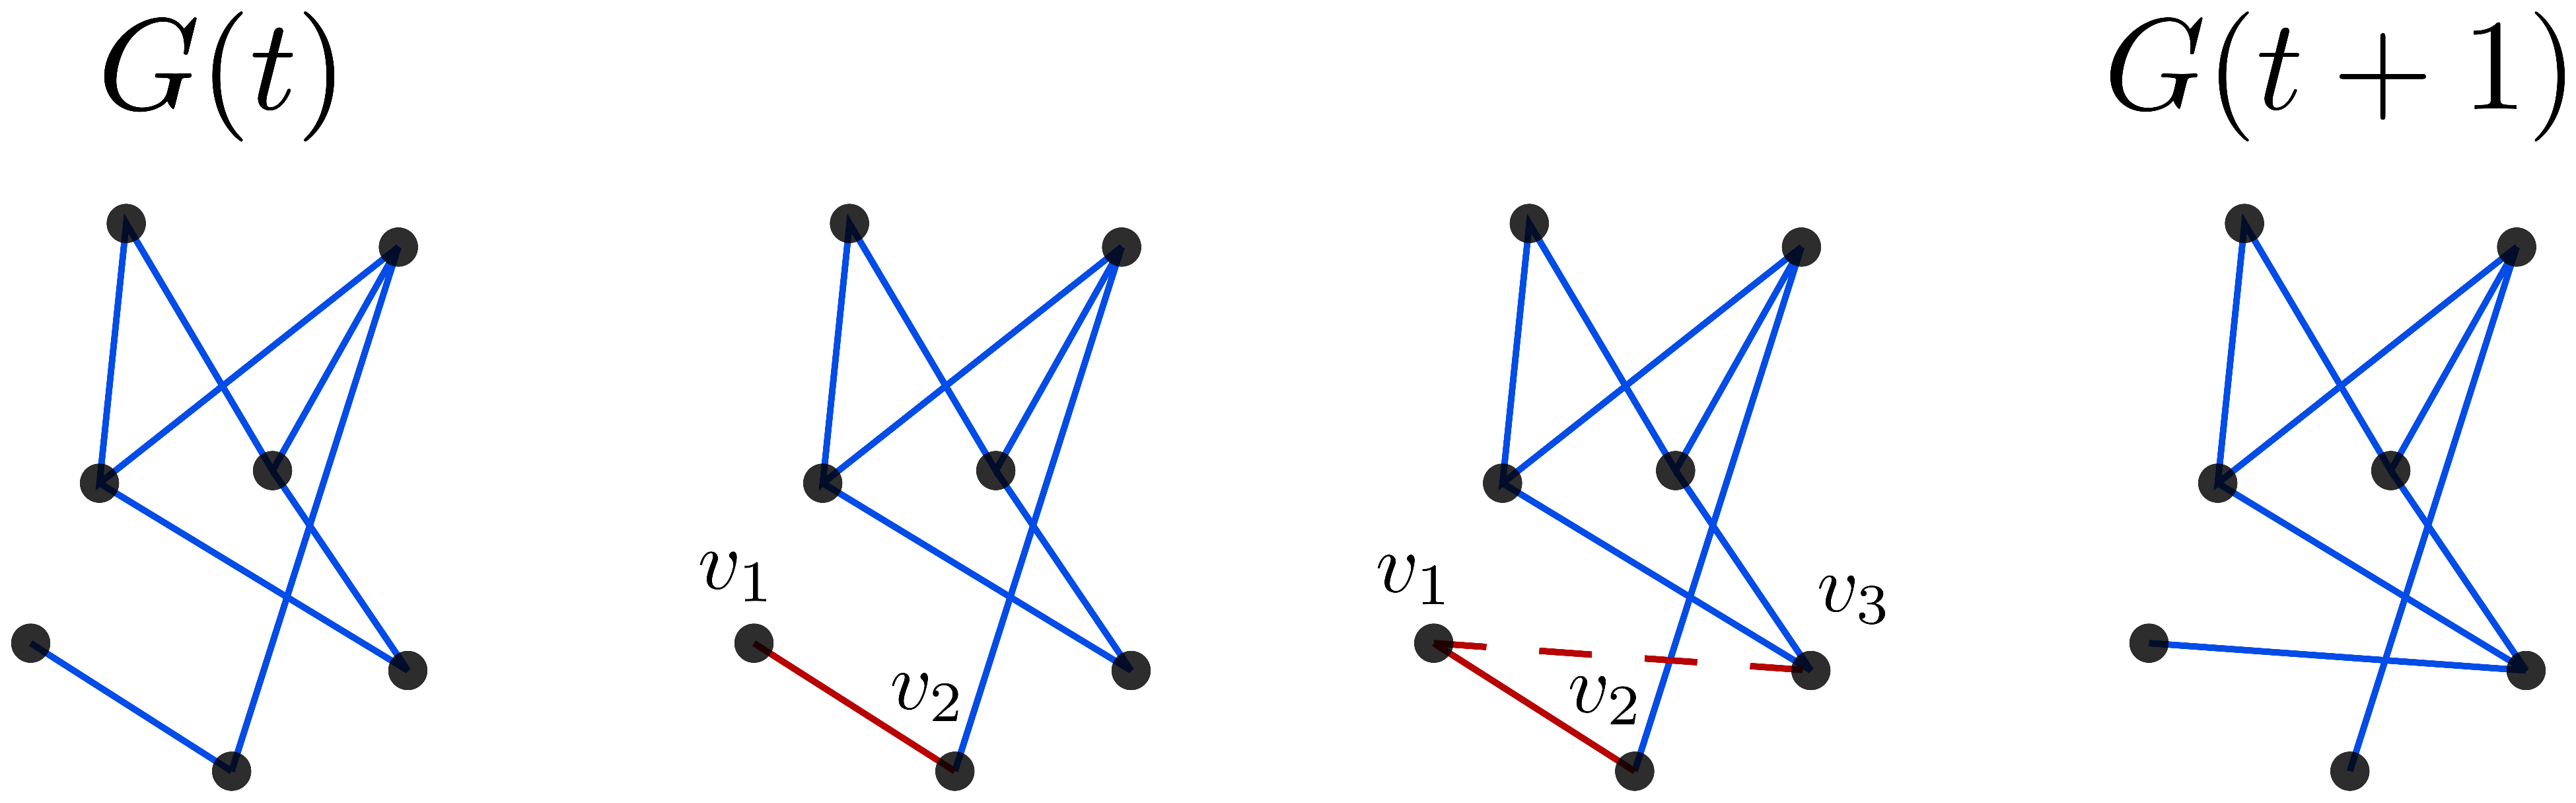
\includegraphics[width=0.9\textwidth]{graph-evo}
    \caption[Schematic of the substeps involved in the multigraph
    evolution dynamics]{Schematic of the substeps of the evolution
      dynamics of the multigraph
      $G(t)$. \label{fig:step-illustration}}
  \end{figure}

  \begin{figure}
    \vspace{-5mm} \centering
    \begin{subfigure}[t]{0.49\textwidth}
      \centering
      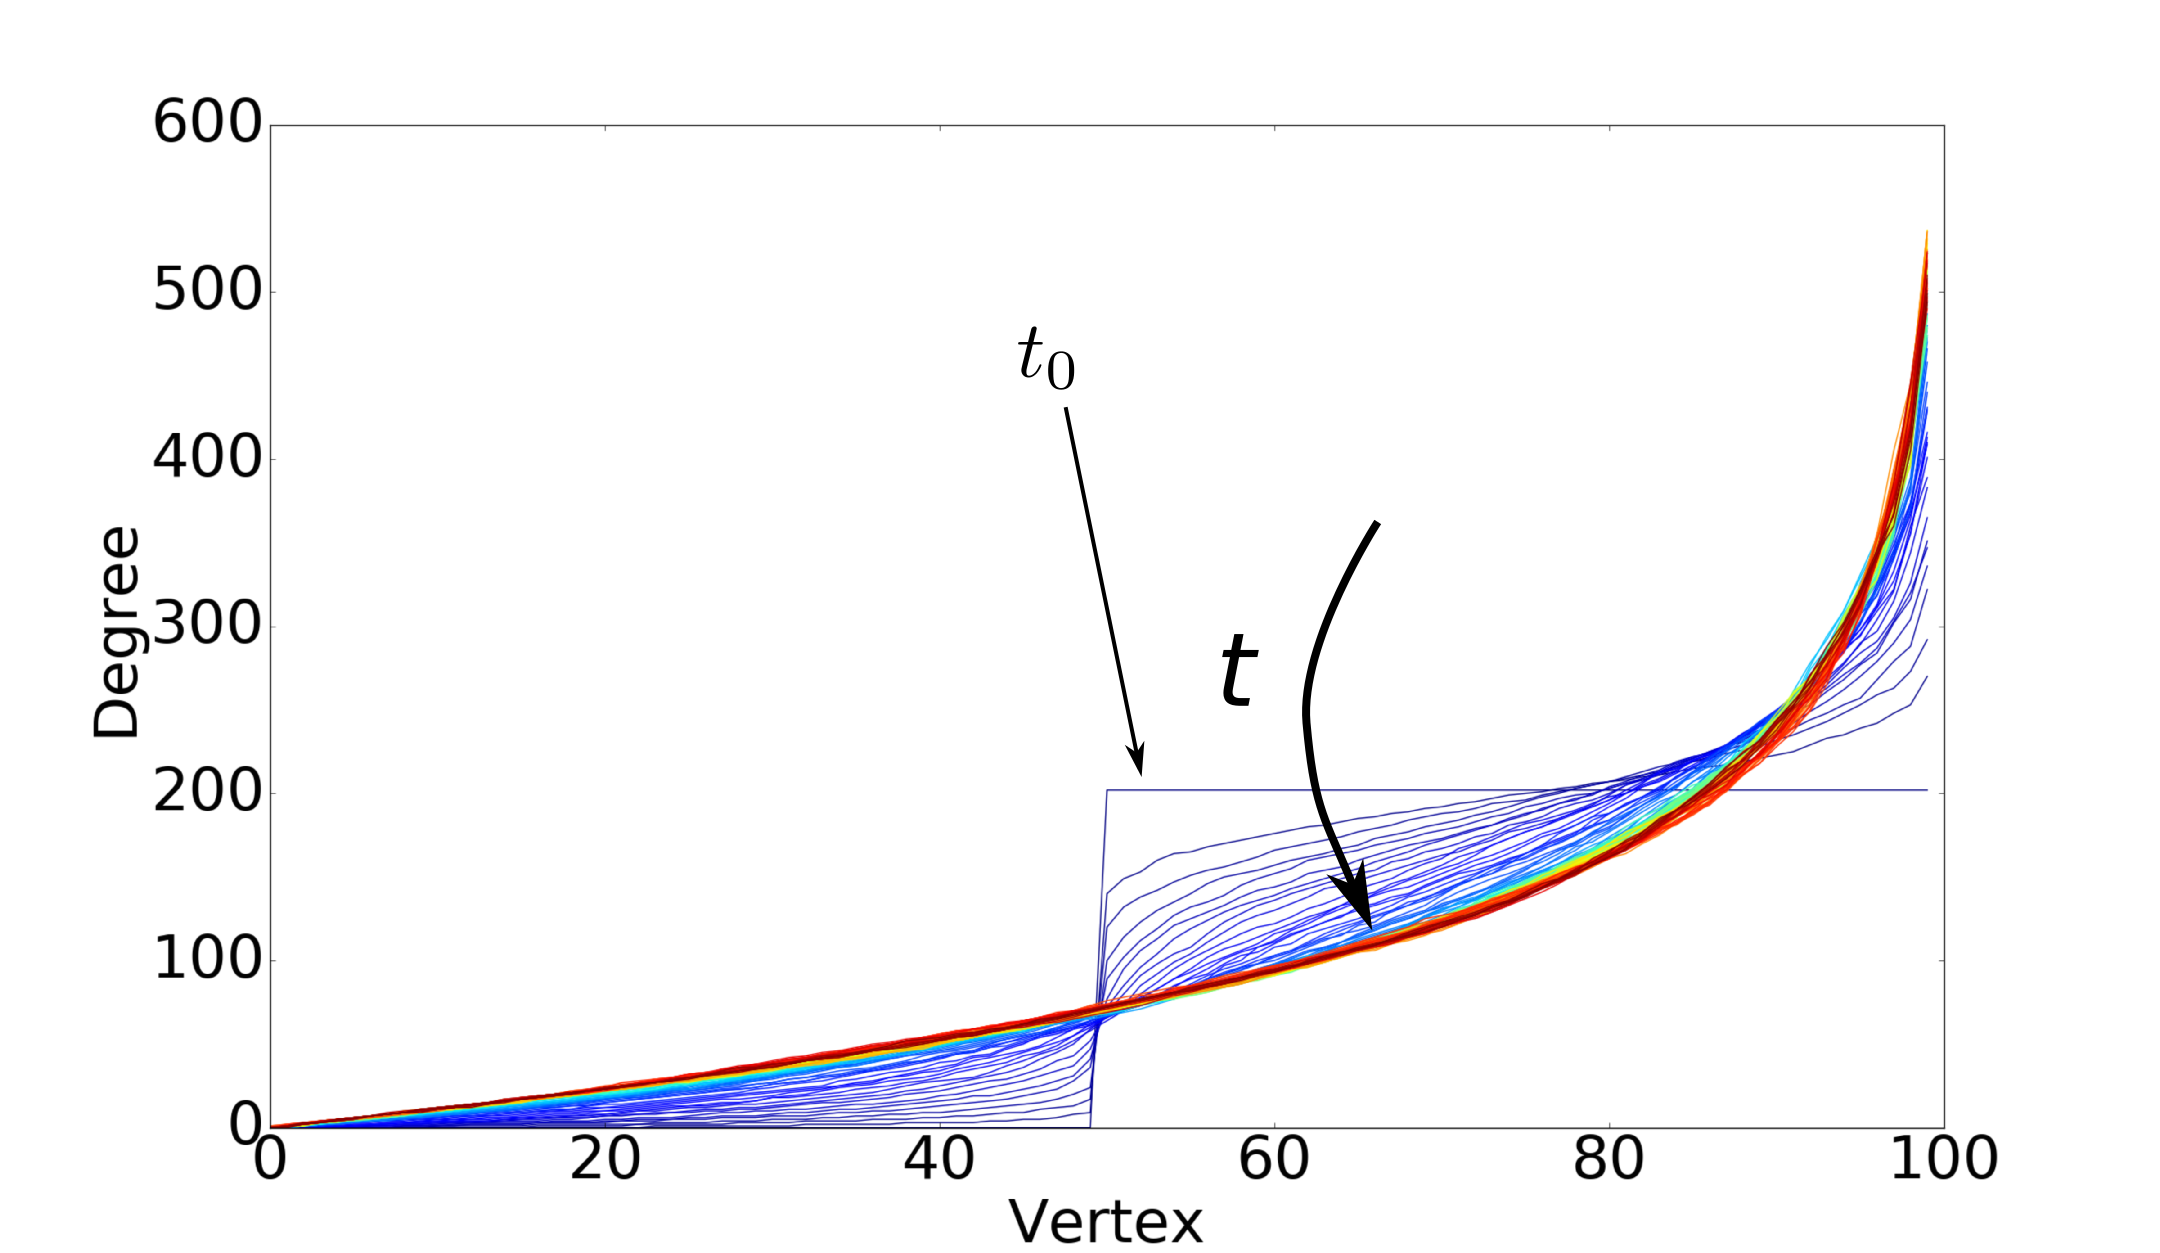
\includegraphics[width=\textwidth]{lopsided-degs-a}
      \subcaption{\label{fig:lopsided-init}}
    \end{subfigure} %
    \begin{subfigure}[t]{0.49\textwidth}
      \centering
      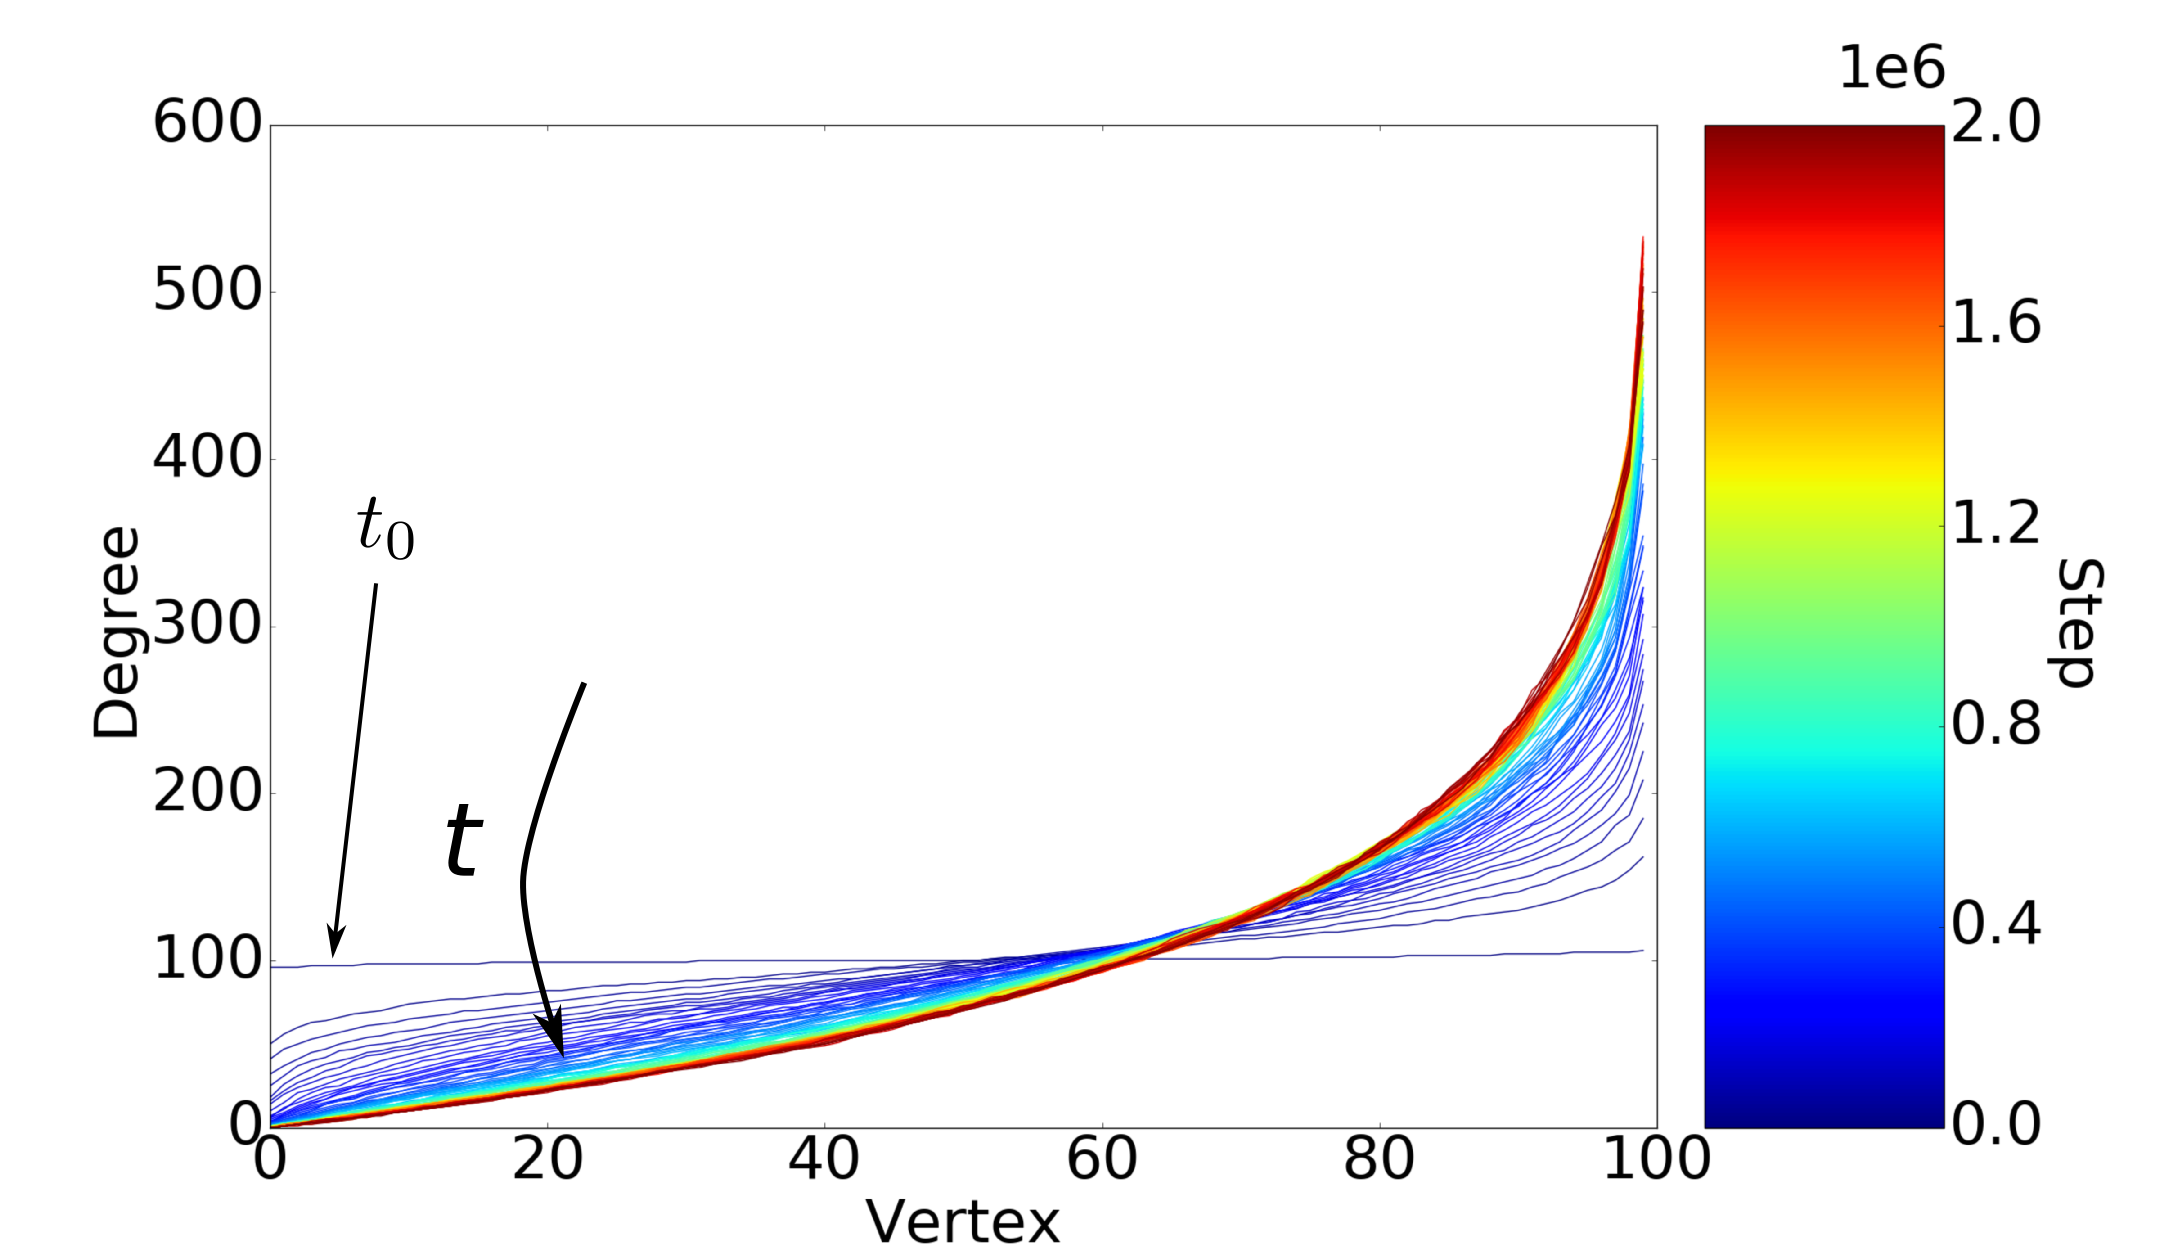
\includegraphics[width=\textwidth]{erdos-degs-a}
      \subcaption{\label{fig:erdos-init}}
    \end{subfigure}
    \caption[Evolution of the multigraph model's sorted degree
    sequence]{Evolution of the multigraph model's sorted degree
      sequence. Two distinct transients are shown, initialized with
      (a) an Erd\H{o}s-R\'{e}nyi random graph with $m = 5,050$ edges
      and (b) a graph in which half the vertices are isolated, and
      half uniformly share $m = 5,050$ edges. Both approach the same
      ultimate stationary sequence. To smoothen the evolution of this
      stochastic system, here we plot the instantaneous average of
      twenty simulations. \label{fig:dse}}
  \end{figure}

  \begin{figure}
    \centering
    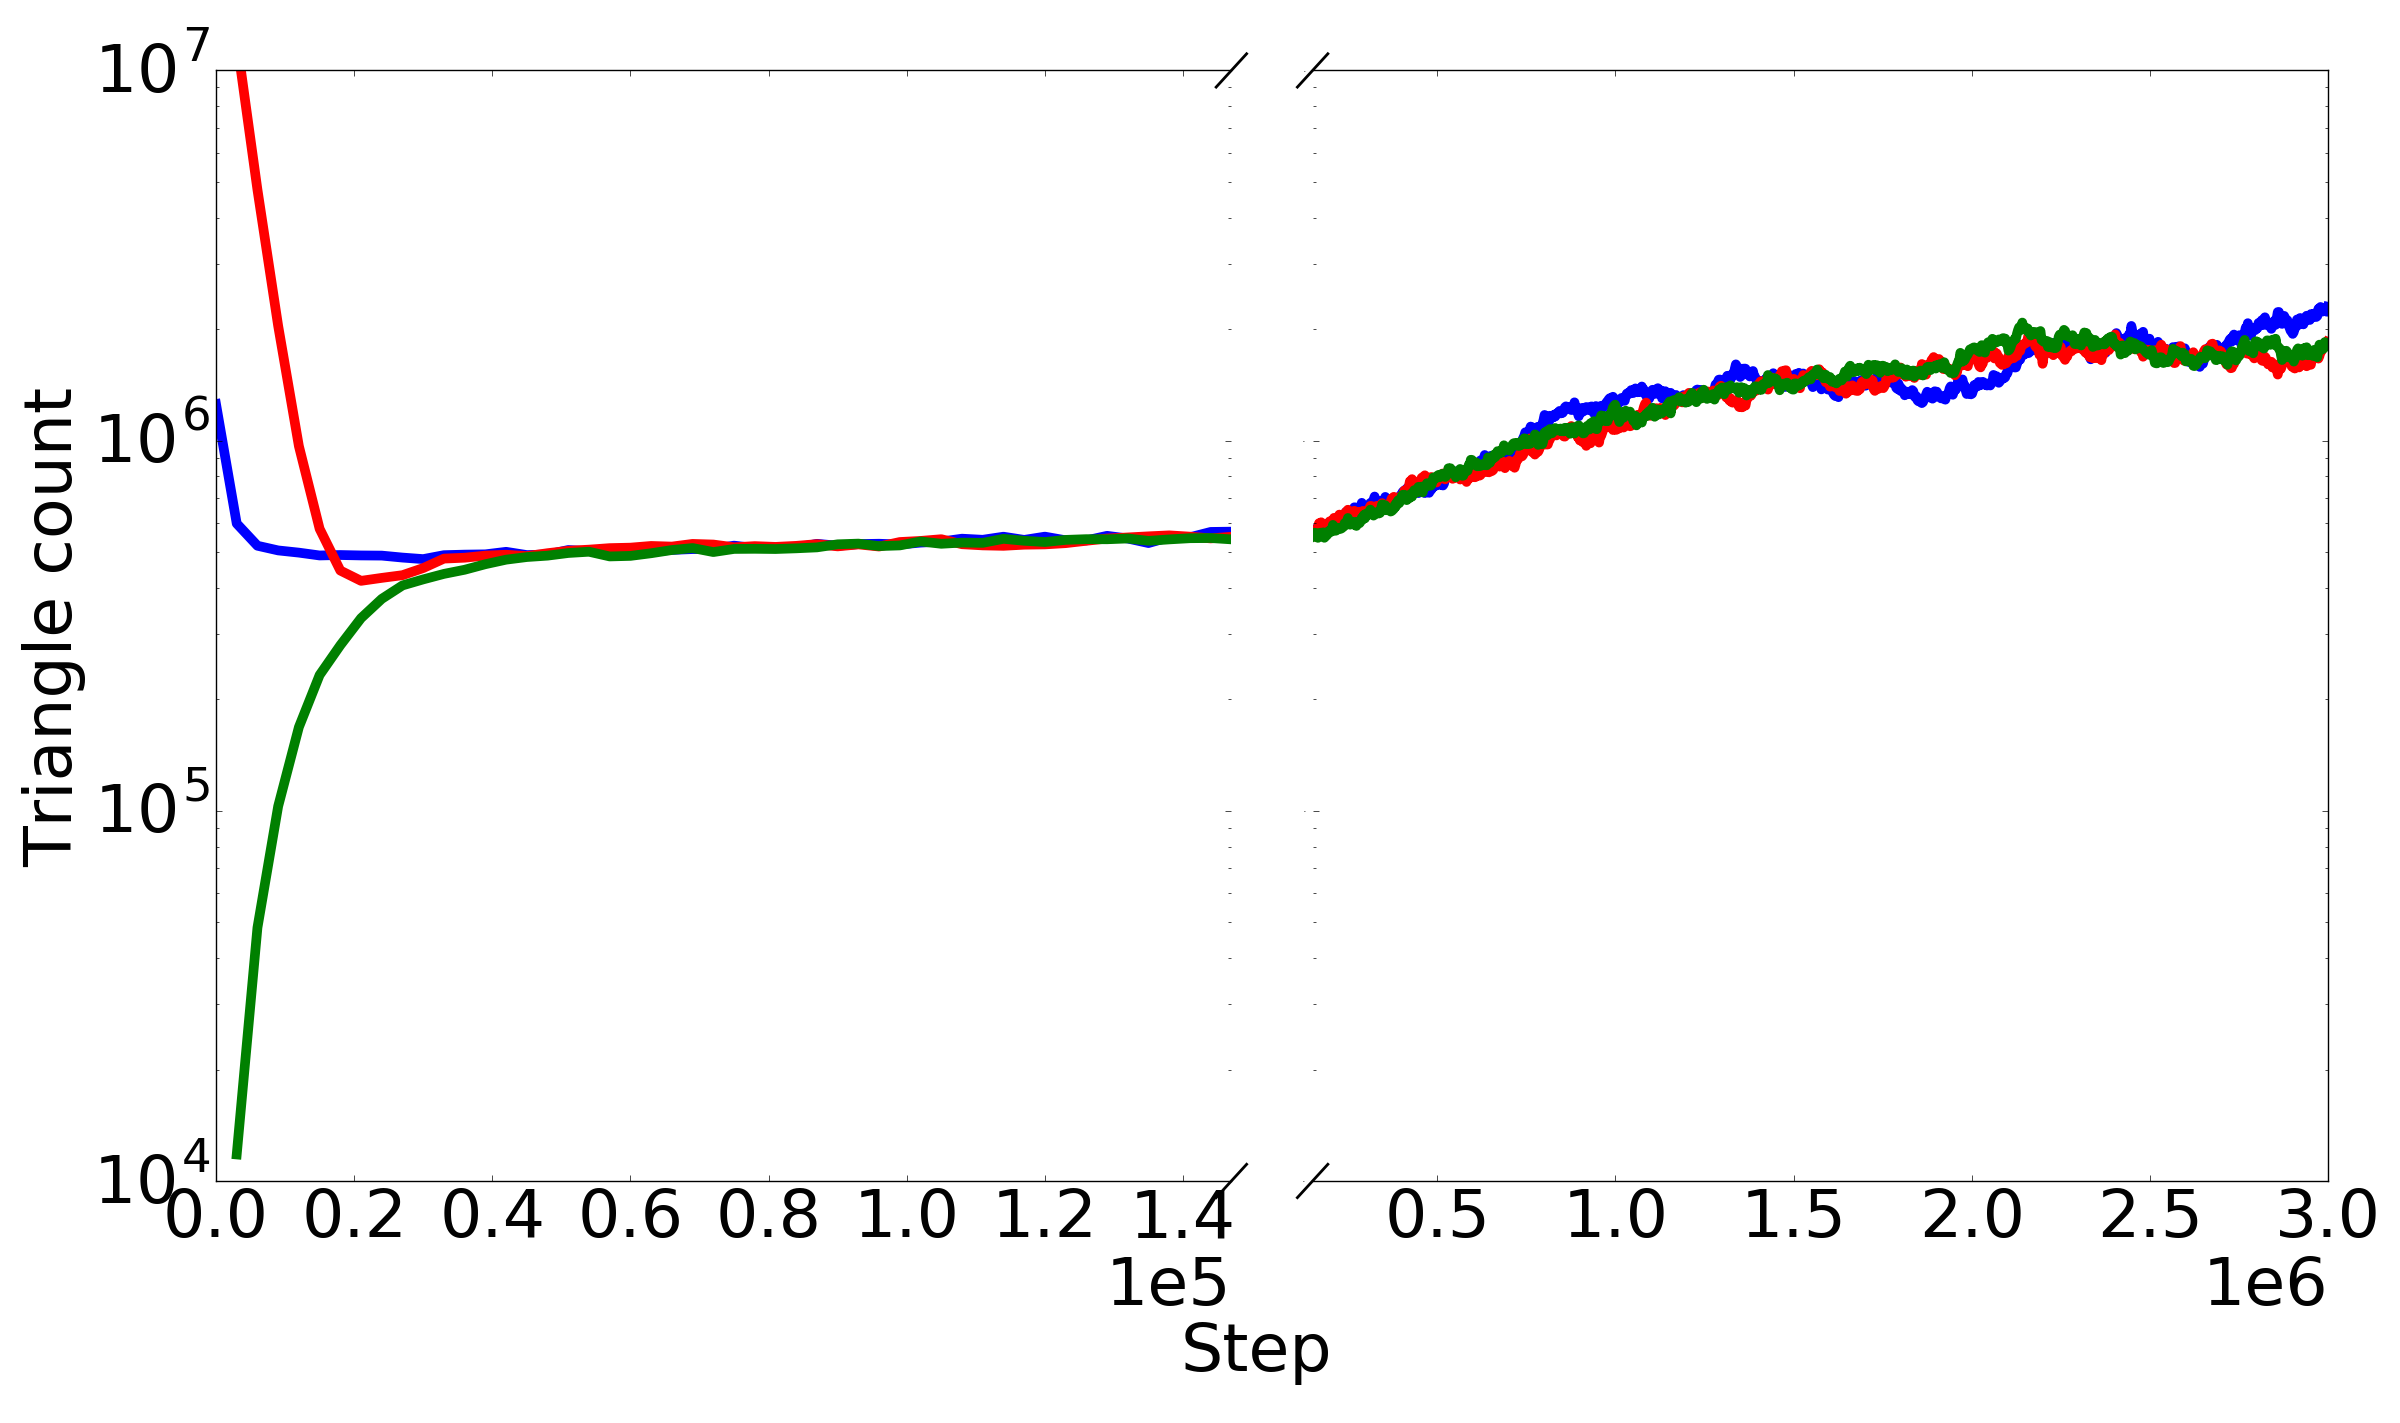
\includegraphics[width=0.8\textwidth]{triangle-slaving-n2-n3}
    \caption[Evolution of triangle count]{Evolution of higher-order
      network statistics (here, the total triangle count) for three
      different network initializations. They are quickly ($O(n^2)$
      steps) drawn to a slow manifold on which they slowly evolve over
      ($O(n^3)$ steps) to a stationary state. \label{fig:sv}}
  \end{figure}

  \section{Equation-free modeling\label{sec:ef}}

  \subsection{Coarse-graining}

  A prerequisite to the implementation of equation-free algorithms is
  the determination of those few, select variables with which one can
  ``close'' a useful approximate description of the coarse-grained
  dynamics of the full, detailed network.
  % 
  This set of variables should clearly be (much) less than those of
  the full system state, and they should evolve smoothly (so, either
  our network would have a large number of nodes, or we would take
  expectations over several realizations of networks with the same
  collective features).
  % 
  Based on the profiles depicted in Fig. (\ref{fig:dse}), the graph's
  degree sequence, (equally informatively, its degree distribution) is
  a good candidate collective observable.
  % 
  It appears to evolve smoothly, while also providing significant
  savings in dimensionality, from an $O(n^2)$ adjacency matrix to a
  length-$n$ vector of degrees. \par

  It now becomes crucial to test whether the evolution of other
  properties of the graph can be correlated to the degree sequence.
  % 
  If not, our current description is incomplete (an equation cannot
  close with only the degree sequence) and there exist other important
  coarse variables that must be included in our macroscopic system
  description.
  % 
  To assess this, we constructed graphs with identical degree
  sequences but varying triangle counts and recorded the evolution of
  this observable under the dynamics prescribed in Section
  \ref{sec:m}. Fig. (\ref{fig:sv}) shows that, within a short time,
  the triangle counts are drawn to an apparent shared ``slow
  manifold'', despite the variation in initial conditions.
  % 
  This supports our selection of the degree sequence as an adequate
  coarse variable to model the system. \par

  Next we describe the other two key elements to equation-free
  modeling which map to and from our microscopic and macroscopic
  descriptions: restriction and lifting operators.

  \begin{figure}
    \centering
    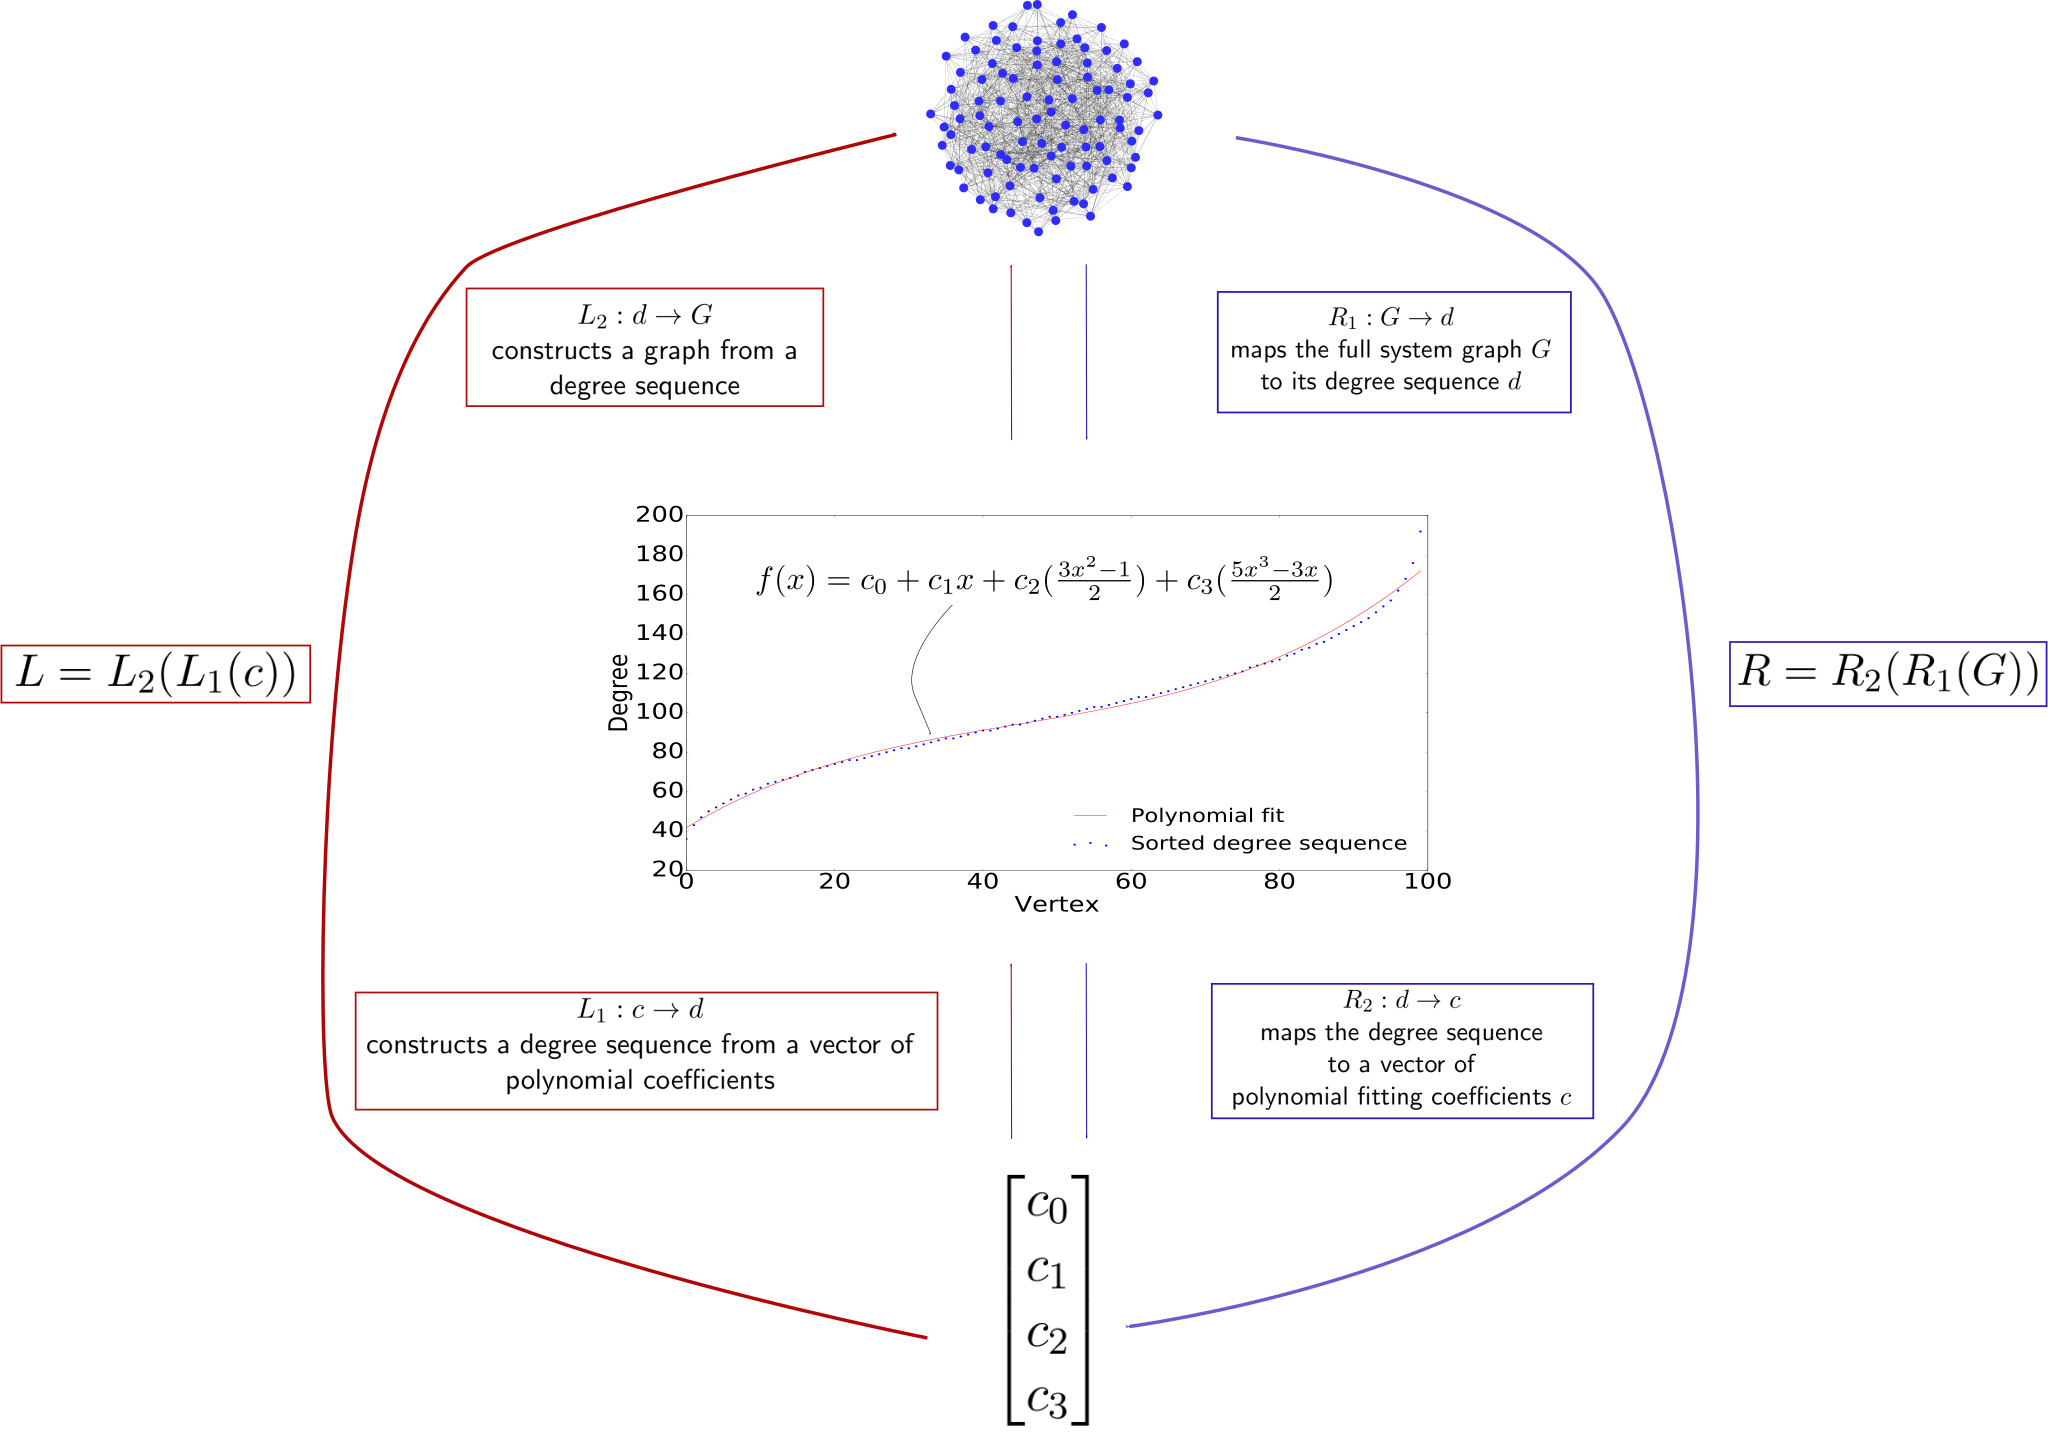
\includegraphics[width=\textwidth]{cpi-diagram}
    \caption[Schematic of multigraph's lifting and restricting
    procedures]{Schematic of our restriction ($\mathbf{R}$) and
      lifting ($\mathbf{L}$) procedures. The graph's sorted degree
      sequence is calculated ($R_1$) and then fit to a third-order
      polynomial ($R_2$). This maps graphs ($G$) to vectors of four
      coefficients ($\mathbf{c}$). To lift, the polynomial is used to
      generate a degree sequence ($L_1$), which is then used to
      construct a consistent graph ($L_2$). This process maps vectors
      of four coefficients ($\mathbf{c}$) to graphs ($G$).
      $\mathbf{R} = R_2 \circ R_1 $ is our restriction and
      $\mathbf{L} = L_2 \circ L_1$ is our
      lifting. \label{fig:cpi-diagram}}
  \end{figure}


  \subsection{Restriction}

  The restriction operator ``translates'' the full network description
  to its corresponding coarse variable values.
  % 
  Here, this involves mapping a multigraph to its sorted degree
  sequence, a simple calculation.
  % 
  However, we may be able to further reduce the dimensionality of our
  coarse system by keeping not the entire length-$n$ degree sequence,
  but rather a low-order polynomial fitting of it.
  % 
  To do so, we first sort the sequence to achieve a smooth,
  monotonically increasing dataset, then fit the result to a
  third-order polynomial, which had been observed to closely
  approximate the sequence evolution throughout time.
  % 
  Our coarse description thus consisted, at every moment in time, of
  the four polynomial coefficient values, specifying a particular
  sorted degree sequence, as shown in Fig. (\ref{fig:cpi-diagram}).
  % 
  The restriction operator therefore maps multigraphs to length-four
  coefficient vectors.
  % 
  This procedure is represented by the blue arrows of
  Fig. (\ref{fig:cpi-diagram}).

  \subsection{Lifting}

  The lifting operator performs the inverse role of restriction:
  translating coarse variables into full networks.
  % 
  This is clearly a one-to-many mapping.
  % 
  Specifically in the context of our model, we map vectors of
  polynomial coefficients to full networks in a two-stage process.
  % 
  First, the coefficient vector is used to recreate a sorted degree
  sequence by evaluating the full polynomial at integer values and
  rounding to the nearest degree, as depicted in
  Fig. (\ref{fig:cpi-diagram}).
  % 
  If the sum of the resulting degree sequence is odd, a single degree
  is added to the largest value to ensure the sequence is graphical.
  % 
  Second, this degree sequence is used as input to any algorithm that
  produces a network consistent with a graphical degree sequence (here
  we typically used a Havel-Hakimi algorithm, creating a graph whose
  degree sequence matches that of the input
  \cite{havel_remark_1955,hakimi_realizability_1962}).
  % 
  While the canonical Havel-Hakimi method produces simple graphs, it
  is not difficult to extend it to multigraphs by allowing the
  algorithm to wrap around the sequence, producing multiple edges and
  self-loops.  The lifting procedure is represented by the red arrows
  of Fig. (\ref{fig:cpi-diagram}).

  \subsection{Coarse projective integration (CPI)}
  \label{sec:cpi}

  The components described above are combined to accelerate
  simulations through Coarse Projective Integration.
  % 
  Denoting the lifting operator by
  $\mathbf{L} \; : \; c \rightarrow G$ where $c \in \mathbb{R}^4$ is
  the vector of polynomial coefficients, and the restriction operator
  as $\mathbf{R} \; : G \rightarrow c$, the algorithm progresses as
  follows:

  \begin{enumerate}
  \item Advance the full system for $t_h$ steps
    \label{cpi:heal}
  \item Continue for $t_c$ steps, restricting the network at intervals
    and recording the coarse variable values
  \item Using the coarse variables collected over the previous $t_c$
    steps, project each variable forward $t_p$ steps with, here, a
    forward-Euler method
    \label{cpi:proj}
  \item With the new, projected coarse variables, lift to one (or more
    copies of) full network
    \label{cpi:init}
  \item Repeat from Step (\ref{cpi:heal}) until the desired time has
    been reached.
  \end{enumerate}

  Note that Step (\ref{cpi:heal}) is intended to allow a singularly
  perturbed quantity to approach its slow manifold.
  % 
  Upon initializing a new full system (here, a new network) in Step
  (\ref{cpi:init}), higher order observables (for example, the
  triangle count) will be far from the values they would attain in a
  detailed simulation.
  % 
  If the coarse system model closes with our chosen variables, then
  either (a) these quantities do not affect the dynamics of the degree
  sequence; or (b) they do, but then by hypothesis these quantities
  quickly evolve to functions of the selected coarse variables (i.e.,
  they approach the slow manifold).
  % 
  In the second case, after a short interval of ``healing'' they will
  be drawn to the expected trajectory, after which we begin sampling.
  % 
  This is analogous to Fig. (\ref{fig:sv}).
  % 
  The computational gains arise from the projective step,
  (\ref{cpi:proj}).
  % 
  Here, we advance the system $t_p$ steps at the cost of one
  evaluation of forward Euler, instead of $t_p$ direct detailed steps.

  Results of the application of this general framework with the
  specific lifting and restriction operators previously outlined are
  shown in Fig. (\ref{fig:cpi-results}). We used an $n=100$-vertex
  graph with $m=50000$ edges and parameter value $\kappa=1$. We ran
  the model for a total of $10 \cdot n^3$ steps, with
  $t_h = 10 \cdot n^2$, $t_c = n^3$ and $t_p = 50 \cdot n^2$.
  % 
  We see good agreement between the CPI-accelerated and normal
  systems, while reducing the number of detailed steps by one third.
  % 
  It is important to mention that this method was applied not to a
  single system instantiation, but to an ensemble of fifty such
  realizations.  This ensured that when properties such as the fitted
  polynomial coefficients were averaged over the ensemble they evolved
  smoothly despite the stochastic nature of the system; in effect, we
  are computing the ``expected network evolution'' averaged over
  consistent realizations.

  \begin{figure}
    \vspace{-5mm} \centering
    \begin{subfigure}{0.59\textwidth}
      \centering
      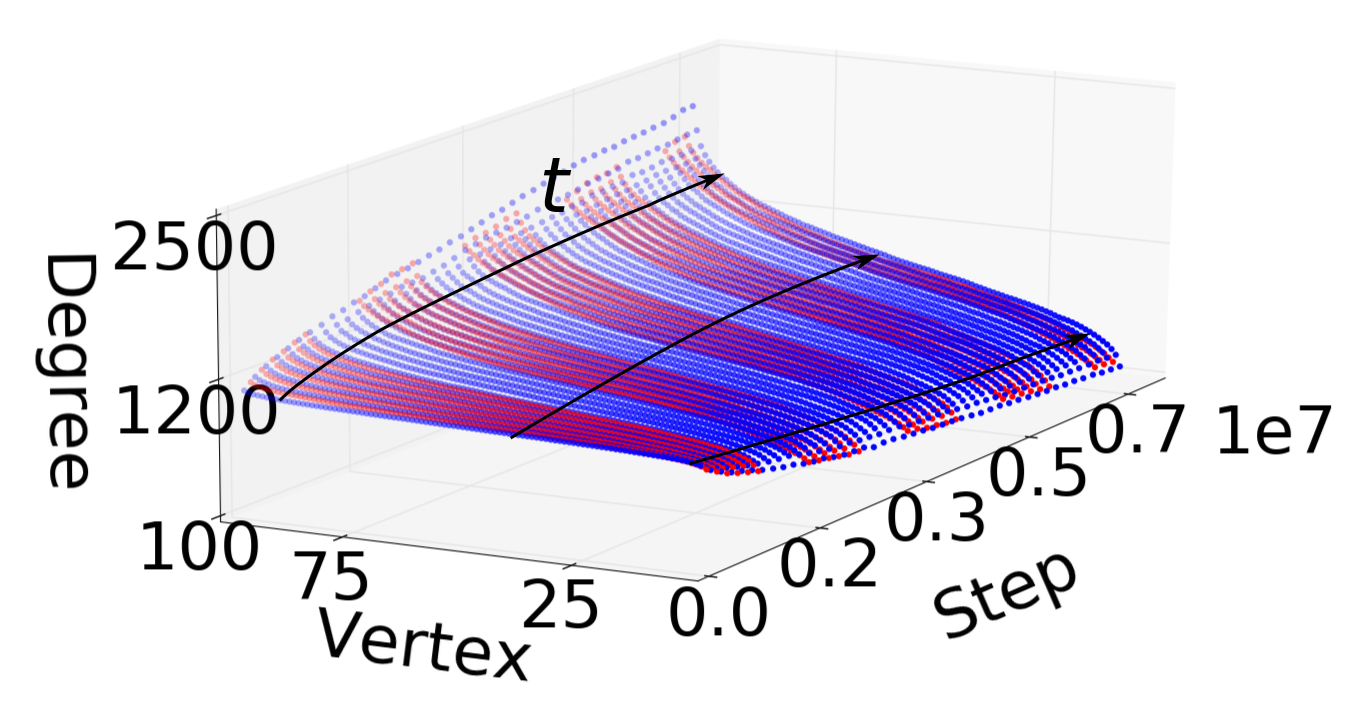
\includegraphics[width=\textwidth]{cpi-3d-comp-stretch}
      \subcaption{\label{fig:cpi-error}}
    \end{subfigure} %
    \begin{subfigure}{0.39\textwidth}
      \centering
      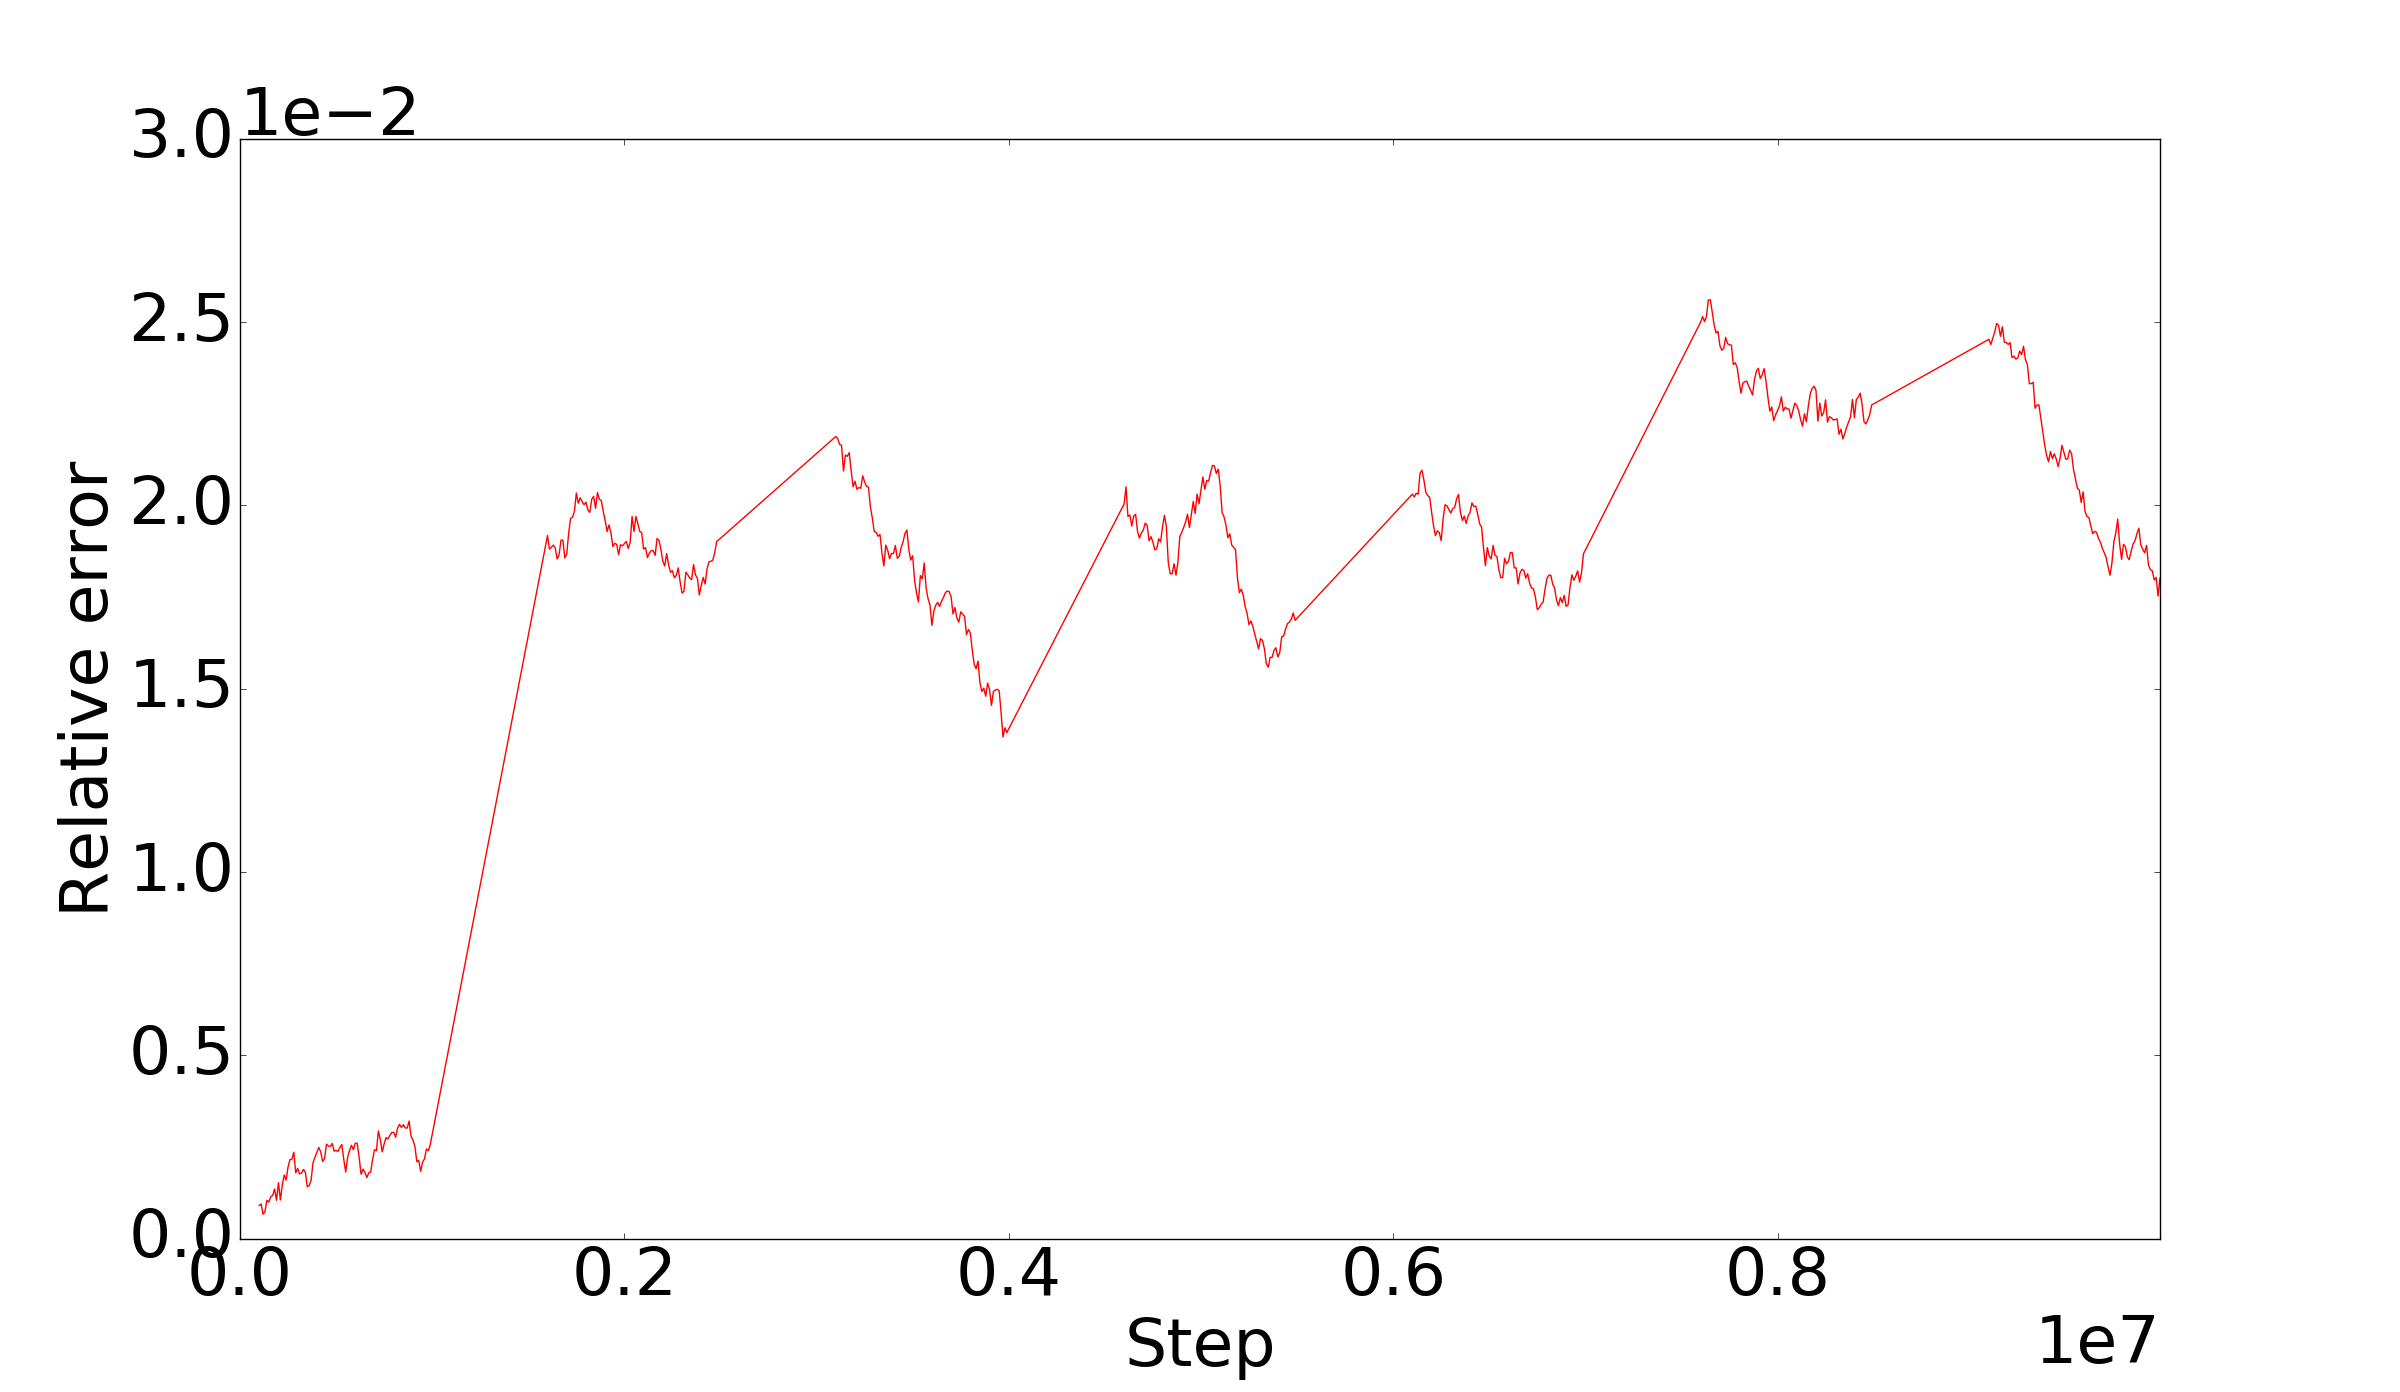
\includegraphics[width=\textwidth]{cpi-relative-error-n3}
      \subcaption{\label{fig:self-error}}
    \end{subfigure}%
    \caption[Coarse-projective integration results]{CPI results: (a)
      the evolution of the CPI-accelerated degree sequence (red)
      compared to direct simulation (blue) and (b) error in
      CPI-accelerated runs calculated by comparing CPI-accelerated
      degree sequences to those arising from an ensemble of direct
      simulations. \label{fig:cpi-results}}
  \end{figure}


  \section{Coarse Newton-GMRES}
  \label{sec:ng}
  Aside from the computational savings of model simulations offered by
  CPI, the equation free framework also permits the calculation of
  system steady states through fixed point (here, matrix-free
  Newton-GMRES) algorithms.
  % 
  Referring back to the CPI procedure outlined in
  Sec. (\ref{sec:cpi}), we can define an operator
  $\Theta: \mathbf{d} \rightarrow \mathbf{d}$ projecting coarse
  variables at $t$ to their values at $t + \delta t$:
  $\mathbf{d}(t+\delta t) =\Theta(\mathbf{d}(t))$.
  % 
  Note that in this section, we take the sorted degree sequence as our
  coarse variable.
  % 
  A system fixed point could then be located by employing Newton's
  method to solve the equation

  \begin{align}
    \label{eq:f}
    \mathbf{F}(\mathbf{d}) \equiv \Theta(\mathbf{d}) - \mathbf{d} = 0
  \end{align}

  However, this requires the repeated solution of the system of linear
  equations
  $DF(\mathbf{d}^{(k)}) \cdot \delta \mathbf{d}^{(k+1)} =
  -\mathbf{F}(\mathbf{d}^{(j)})$, in which the system Jacobian, $DF$
  is unavailable.
  % 
  Thankfully, we may circumvent this obstacle by estimating the
  directional derivatives $DF(\mathbf{d}) \cdot \delta \mathbf{d}$ via
  a difference approximation of the form

  \begin{align}
    DF(d) \cdot \delta \mathbf{d} \approx \frac{\| \delta \mathbf{d} \| \mathbf{F}(\mathbf{d} + h \| \mathbf{d} \| \frac{\delta \mathbf{d}}{\| \delta \mathbf{d} \|}) - \mathbf{F}(\mathbf{d})}{h \| \mathbf{d} \|}
  \end{align}

  \noindent for nonzero $\mathbf{d}$, which in turn is evaluated
  through calls to $\mathbf{F}$ as defined in Eq. (\ref{eq:f})

  This is precisely the approach of the Newton-GMRES method, in which
  the solution to a linear system is sought for in expanding Krylov
  subspaces \cite{kelley_solving_2003}.
  % 
  Applying this algorithm in conjunction with the $\Theta$ operator
  defined in Sec. (\ref{sec:cpi}) allowed us to locate the stationary
  distribution without simply running and observing the full system
  for long times, as would otherwise be required.
  % 
  Results are shown in Fig. (\ref{fig:newton-results}).
  % 
  We note that coarse stability results can also be obtained via an
  iterative Arnoldi eigensolver, again estimating matrix-vector
  products as above.

  \begin{figure}
    \vspace{-5mm} \centering
    \begin{subfigure}{0.49\textwidth}
      \centering
      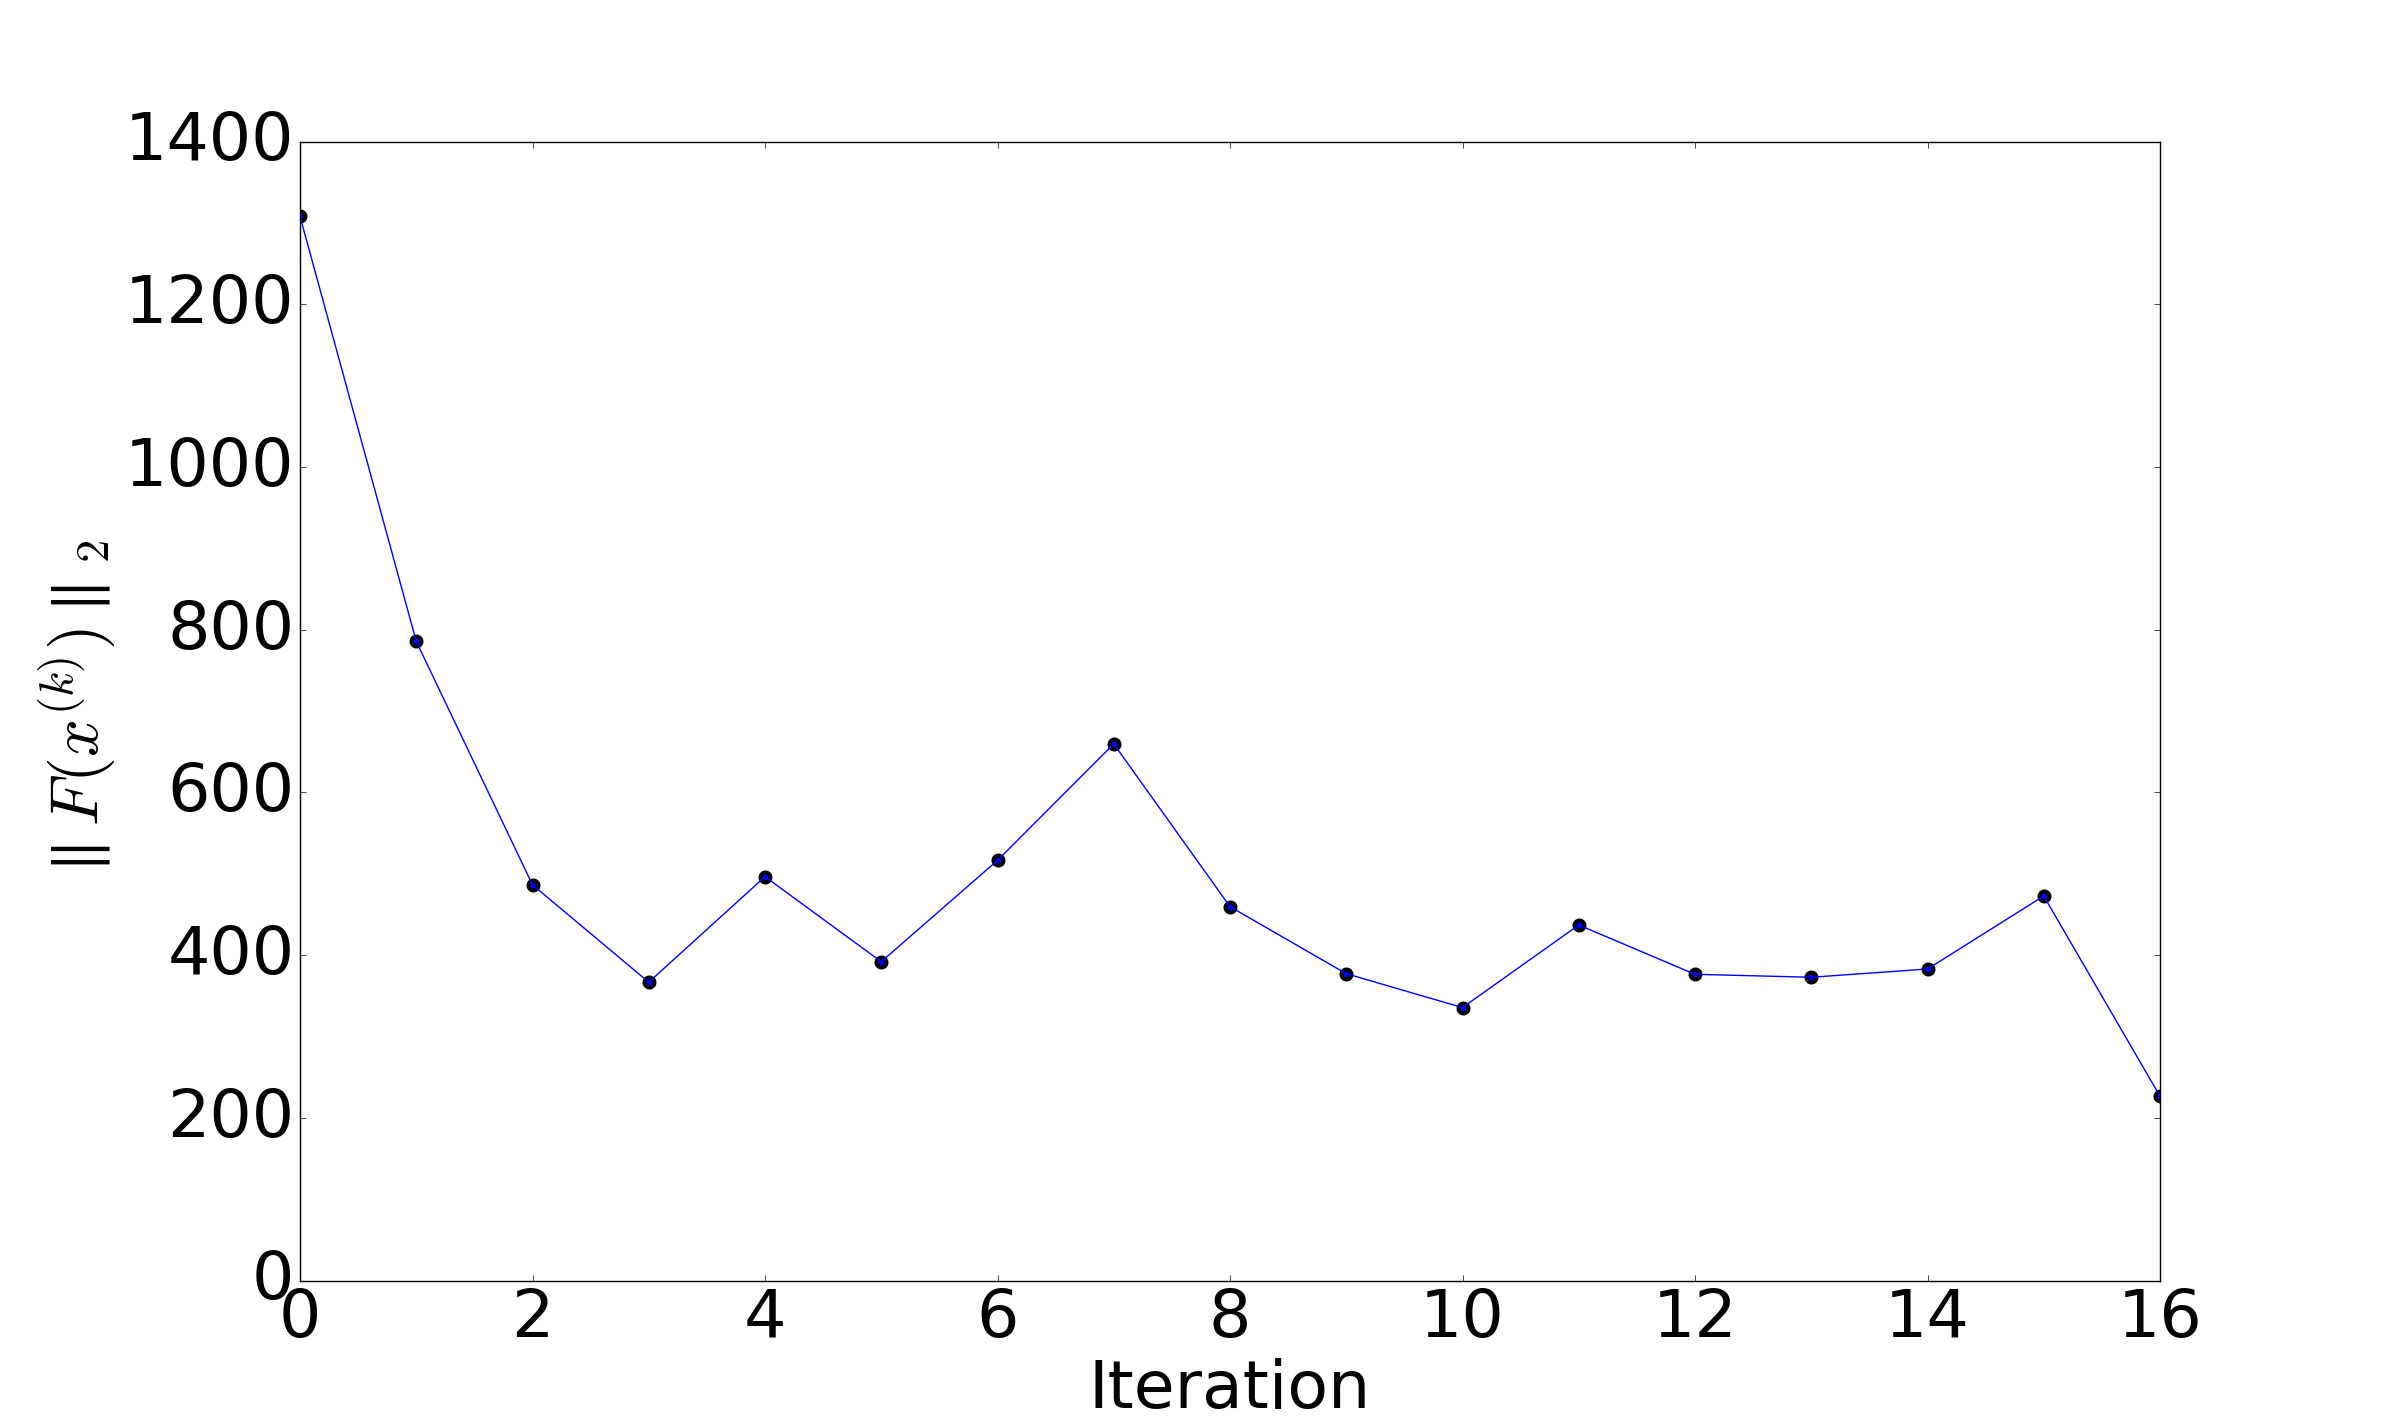
\includegraphics[width=\textwidth]{newton-error}
      \subcaption{\label{fig:newton-error}}
    \end{subfigure} %
    \begin{subfigure}{0.49\textwidth}
      \centering
      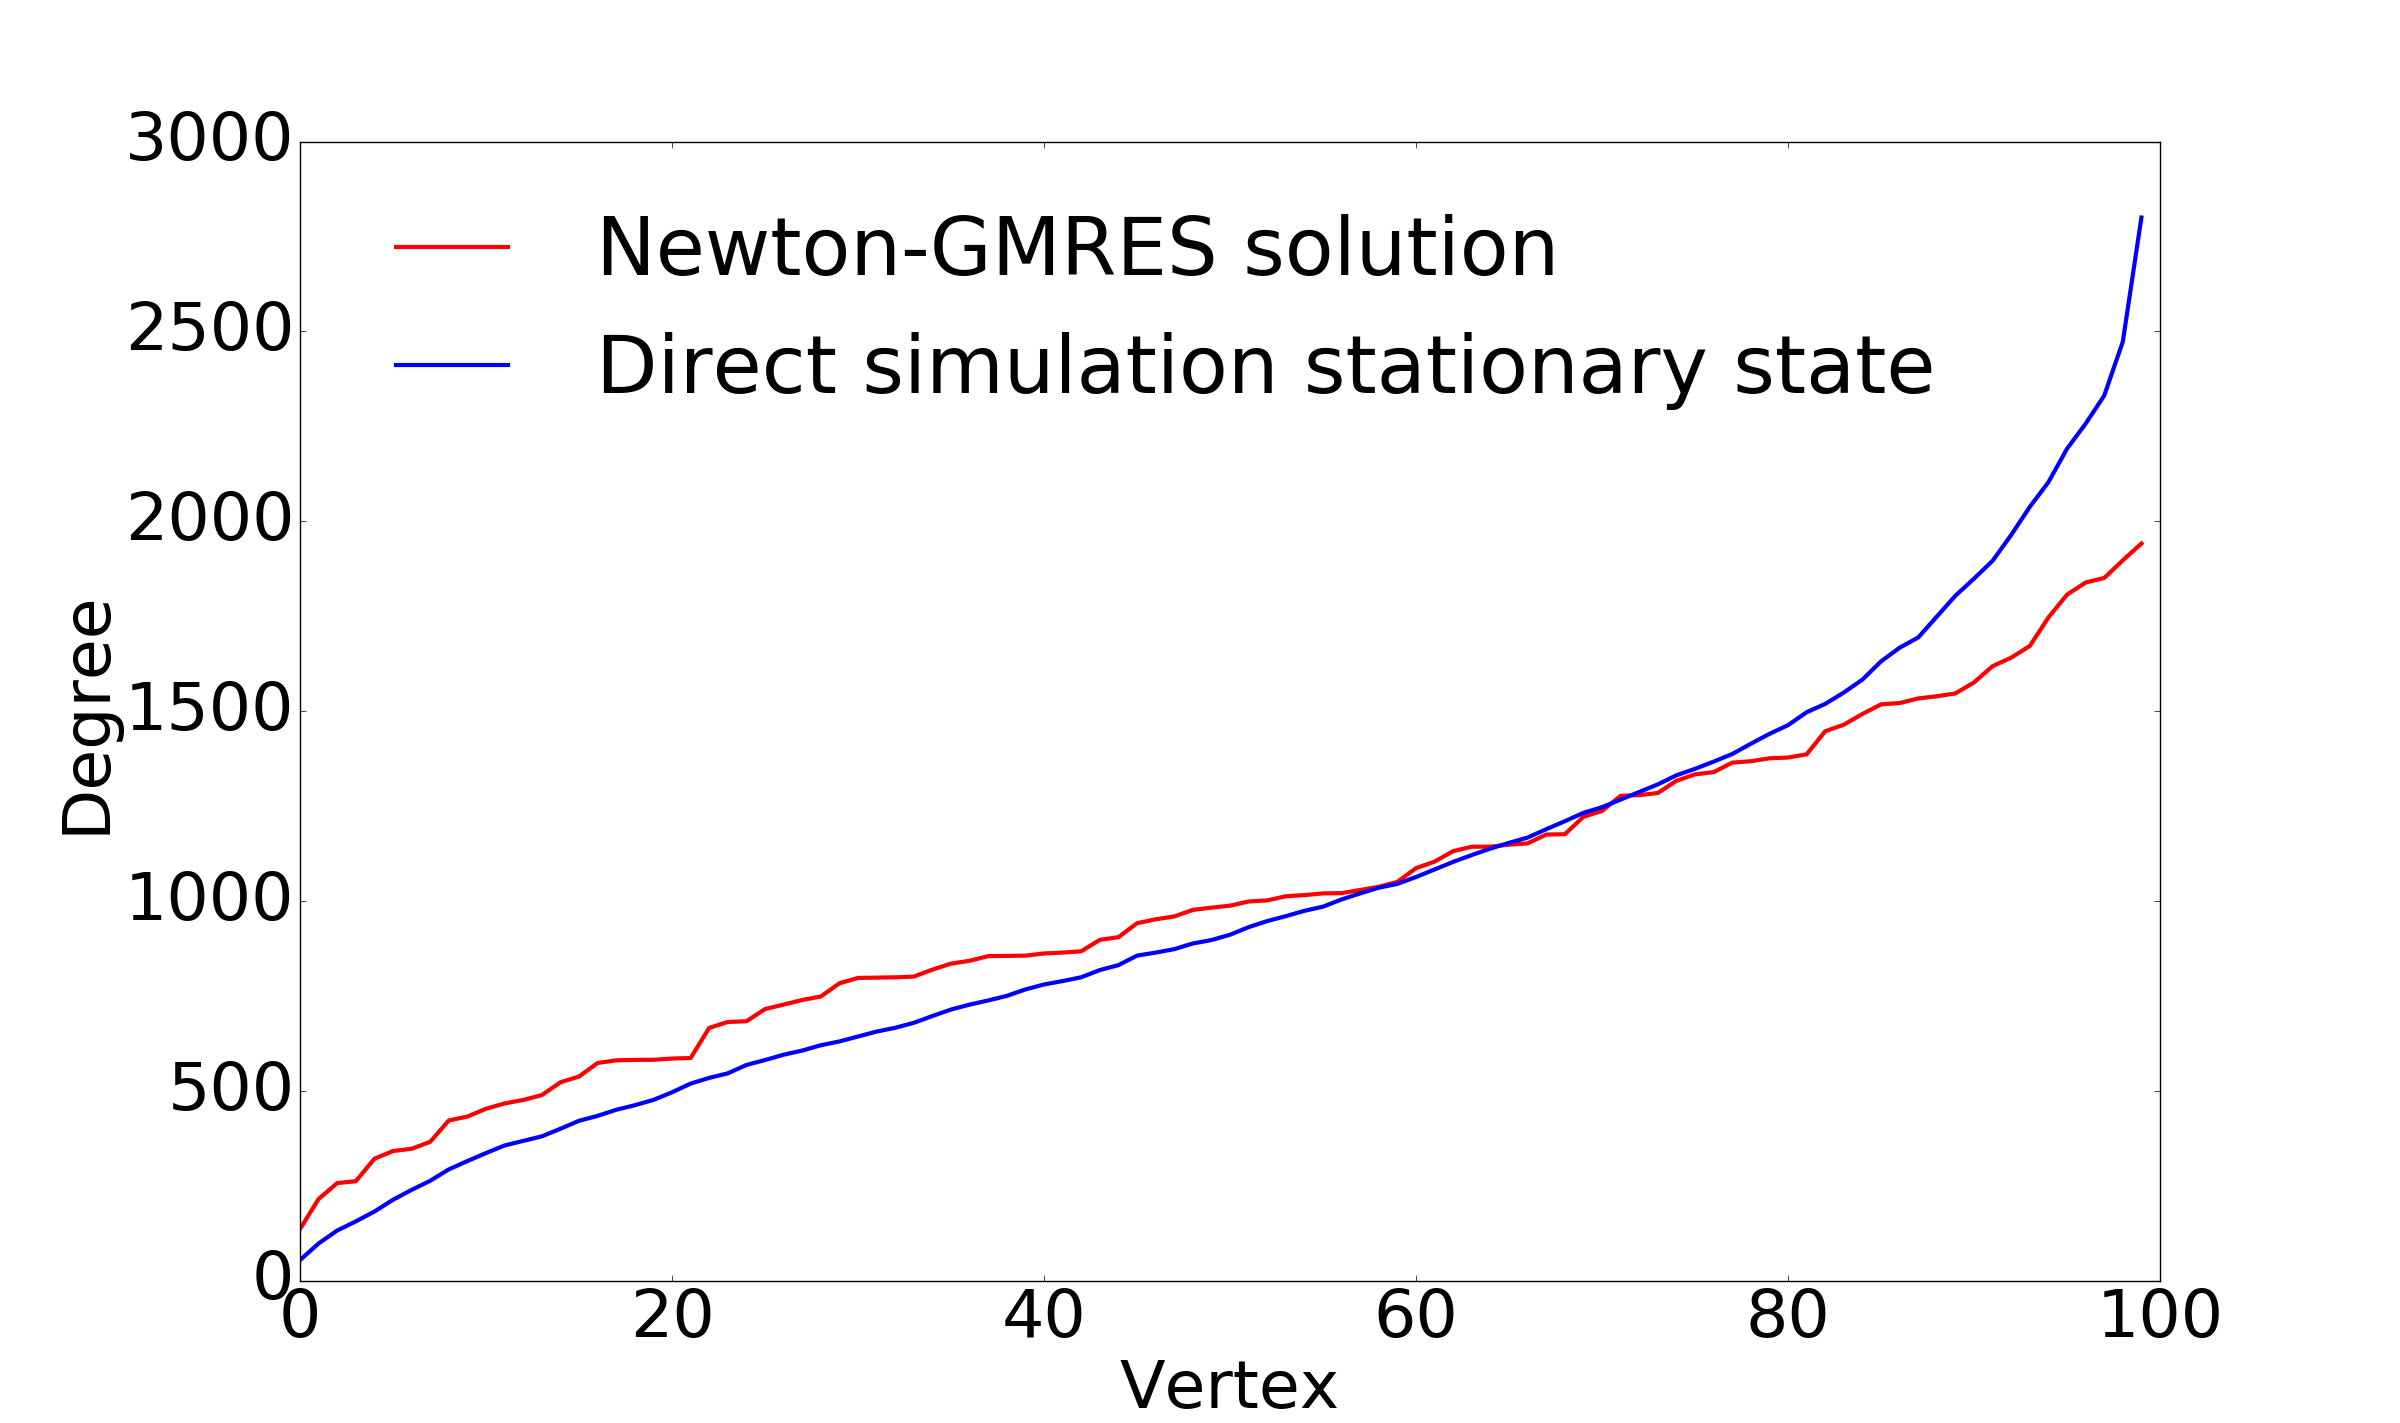
\includegraphics[width=\textwidth]{newton-comp}
      \subcaption{\label{fig:newton-comp}}
    \end{subfigure}%
    \caption[Coarse Newton-GMRES results]{Coarse Newton-GMRES results:
      (a) evolution of the error in the coarse Newton-GMRES iteration
      scheme; and (b) visual comparison of the algorithm's solution to
      the stationary state obtained from direct
      simulation. \label{fig:newton-results}}
  \end{figure}


  \section{Algorithmic coarse-graining}
  \label{sec:dr}
  Crucial to the above analysis was the determination of suitable
  coarse, system variables: it is the starting point of any equation
  free method.
  % 
  However, the discovery of such a low-dimensional description is
  highly non-trivial.
  % 
  Currently, as in this paper, they are ``discovered through informed
  experience'': through careful investigation of direct simulations,
  and knowledge of previous analytical results.
  % 
  Clearly, any process which could algorithmically guide this search
  based on only simulation data would be of great benefit to the
  modeling practitioner.
  % 
  We now illustrate two such algorithms: principal component analysis
  (PCA) and diffusion maps (DMAPS).
  % 
  First, we briefly discuss some aspects of the important issue of
  defining distances between networks, a prerequisite for any
  dimensionality-reduction technique.

  \subsection{On network distances}

  When applying dimensionality reduction techniques to a dataset, it
  is necessary to define a distance (or similarity) between each pair
  of data points.
  % 
  If these points are a set of vectors in $\mathbb{R}^n$ one has a
  number of metrics to choose from, the Euclidean distance being a
  common first option.
  % 
  Unfortunately, when individual points are not vectors but networks,
  the definition of a useful and computationally easily quantified
  metric becomes far more challenging.
  % 
  Examples such as the maximal common subgraph and edit distances,
  defined in \cite{bunke_graph_1998} and \cite{gao_survey_2010} define
  metrics on the space of graphs, but their computation is
  $NP\textnormal{-}hard$.
  % 
  Other computationally feasible approaches include comparing
  distributions of random walks on each graph
  \cite{vishwanathan_graph_2010}, calculating the so-called $n$-tangle
  density \cite{gallos_revealing_2014}, or calculating the edit
  distance
  with an approximation algorithm \cite{riesen_approximate_2009,zeng_comparing_2009}.

  The strategy used in the following computations, detailed in
  \cite{rajendran_analysis_2013} and \cite{xiao_structure-based_2008},
  enumerates the number of times a certain set of motifs (or
  subgraphs) appears in each network in the dataset.
  % 
  This maps each network to a vector in $\mathbb{R}^n$, and the
  Euclidean distance is subsequently used to quantify the similarity
  of two graphs.
  % 
  Due to computational restrictions, we chose here to only count the
  number of three- and four-vertex single-edge subgraphs contained in
  each network.
  % 
  As there are eight such motifs, shown in Fig. (\ref{fig:motifs}),
  this process $\gamma$ maps each graph to an eight-dimensional
  vector: $\gamma : G \rightarrow \mathbb{R}^8$.
  % 
  We applied this operation to a simplified version of each graph,
  wherein any multiple edges were reduced to a single edge.

  \begin{figure}
    \vspace{-5mm} \centering
    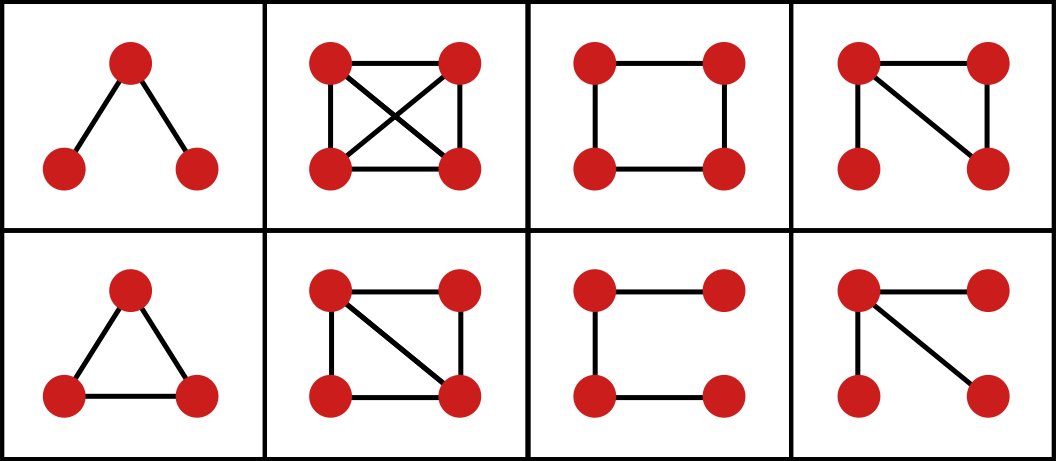
\includegraphics[width=\textwidth]{motifs}
    \caption[List of subgraphs used to embed multigraphs]{List of the
      single-edge subgraphs used to embed each network.  The number of
      times each appeared in the simplified input graph was
      calculated, mapping input graphs to
      $\mathbb{R}^8$. \label{fig:motifs}}
  \end{figure}

  \subsection{PCA\label{sec:pca}}
  

  PCA is used to embed data into linear subspaces that capture the
  directions along which the data varies most
  \cite{jolliffe_principal_2014}.
  % 
  Given some matrix $X \in \mathbb{R}^{n \times m}$ in which each of
  the $m$ column vectors $x_i$ represents a different collection of
  the $n$ system variables (i.e. a different data point), PCA computes
  a reduced set of $k<n$, orthogonal ``principal components''
  $z_i \in \mathbb{R}^n$ that constitute an optimal basis for the data
  in the sense that, among linear, $k$-dimensional embeddings,
  $w_i = Z^Tx_i$ captures the maximum possible variance in the
  dataset, where
  $Z = \begin{bmatrix} | & | & & | \\ z_1 & z_2 & \hdots & z_k \\ | &
    | & & | \end{bmatrix}$.
  % 
  This approach has found wide application, but can suffer from its
  inability to uncover simple \textit{nonlinear} relationships among
  the input variables.
  % 
  Indeed, many datasets will not ``just lie along some hyperplane''
  embedded in $\mathbb{R}^n$, but will rather lie on a low-dimensional
  nonlinear manifold throughout the space.

  Theoretical results in \cite{rath_time_2012} state that, for a given
  network size $n$, the final stationary state depends only on the
  number of edges present $m$ and the model parameter $\kappa$.
  % 
  To assess both the validity of our graph embedding technique and the
  usefulness of PCA in the context of complex networks, we generated a
  dataset of stationary states over a range of $m \in [50, 5000]$ and
  $\log(\kappa) \in [0, 2]$ values by directly running the model over
  $2n^3$ steps ($N=30$ values of each parameter were taken, for a
  total of $900$ networks).
  % 
  We fixed the network size to $n=50$ vertices.
  % 
  Each resulting graph $G(m_i, \kappa_j) = G_{ij}$ was then embedded
  into $\mathbb{R}^8$ by counting the number of times each of the
  subgraphs shown in Fig. (\ref{fig:motifs}) appeared in the network.
  % 
  Thus $\gamma(G_{ij}) = v_{ij} \in \mathbb{R}^8$.
  % 
  We then proceeded to perform a principal component analysis on this
  collection of vectors $\{v_{ij}\}_{i,j=1}^N$.
  % 
  Interestingly, the first two principal components $z_1$ and $z_2$
  succeeded in uncovering a two-dimensional embedding of the dataset
  corresponding to the two underlying parameters $m$ and $\kappa$, as
  shown in Fig. (\ref{fig:pca}) in which the data is projected on the
  plane spanned by these two vectors.
  % 
  This suggests that, given some final network state $G(m, \kappa)$,
  by projecting its embedding onto these first two principal
  components one could obtain a reasonable approximation of the hidden
  parameter $\kappa$.

  \begin{figure}
    \vspace{-5mm} \centering
    \begin{subfigure}{0.49\textwidth}
      \centering
      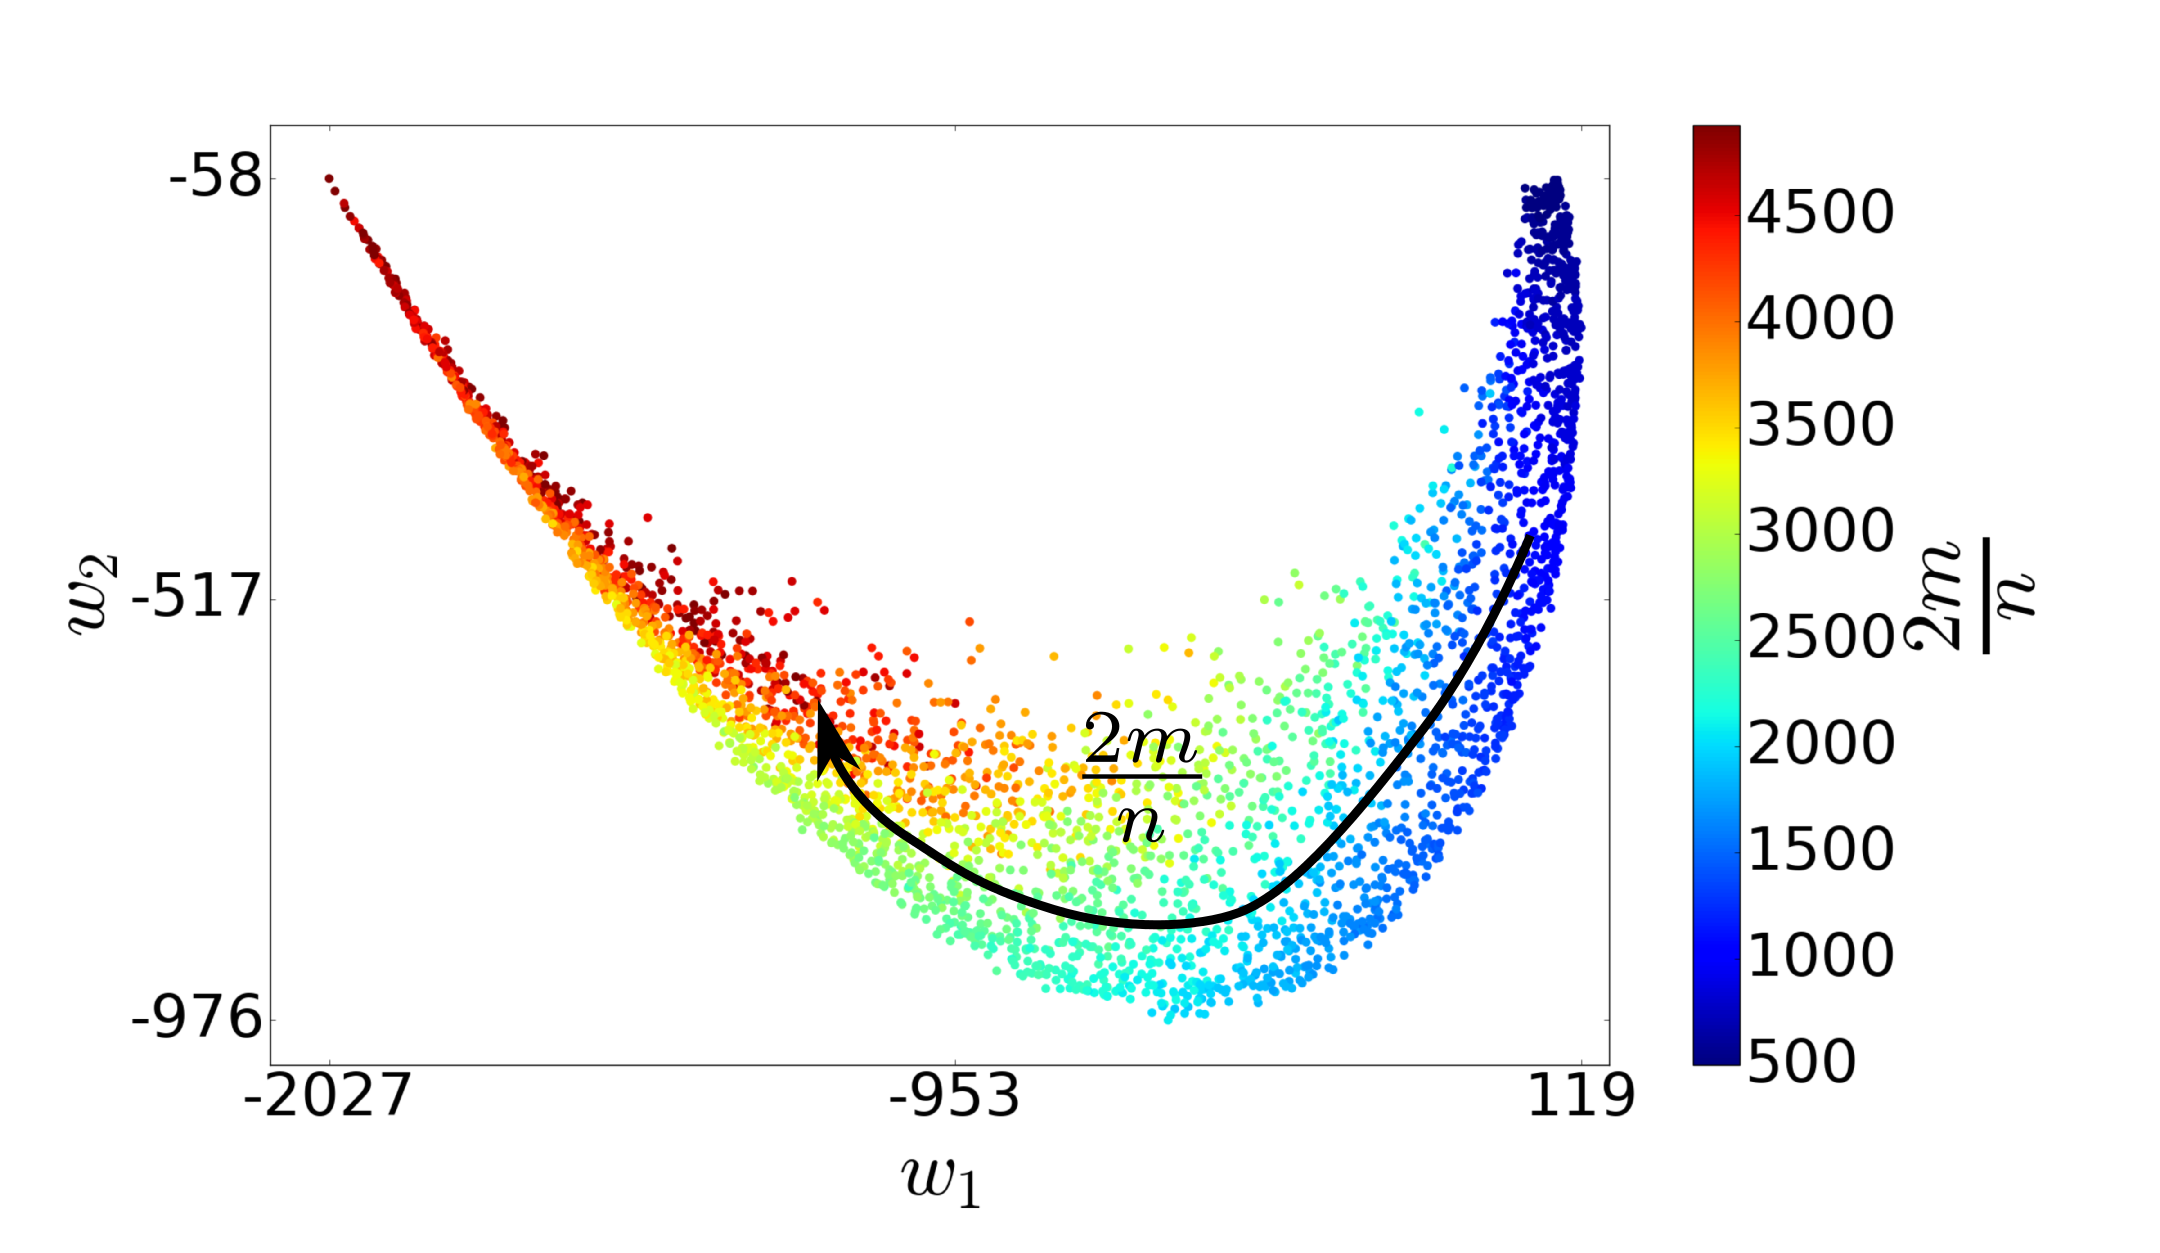
\includegraphics[width=\textwidth]{pca-2d-rho-a}
      \subcaption{\label{fig:pca-rho}}
    \end{subfigure} %
    \begin{subfigure}{0.49\textwidth}
      \centering
      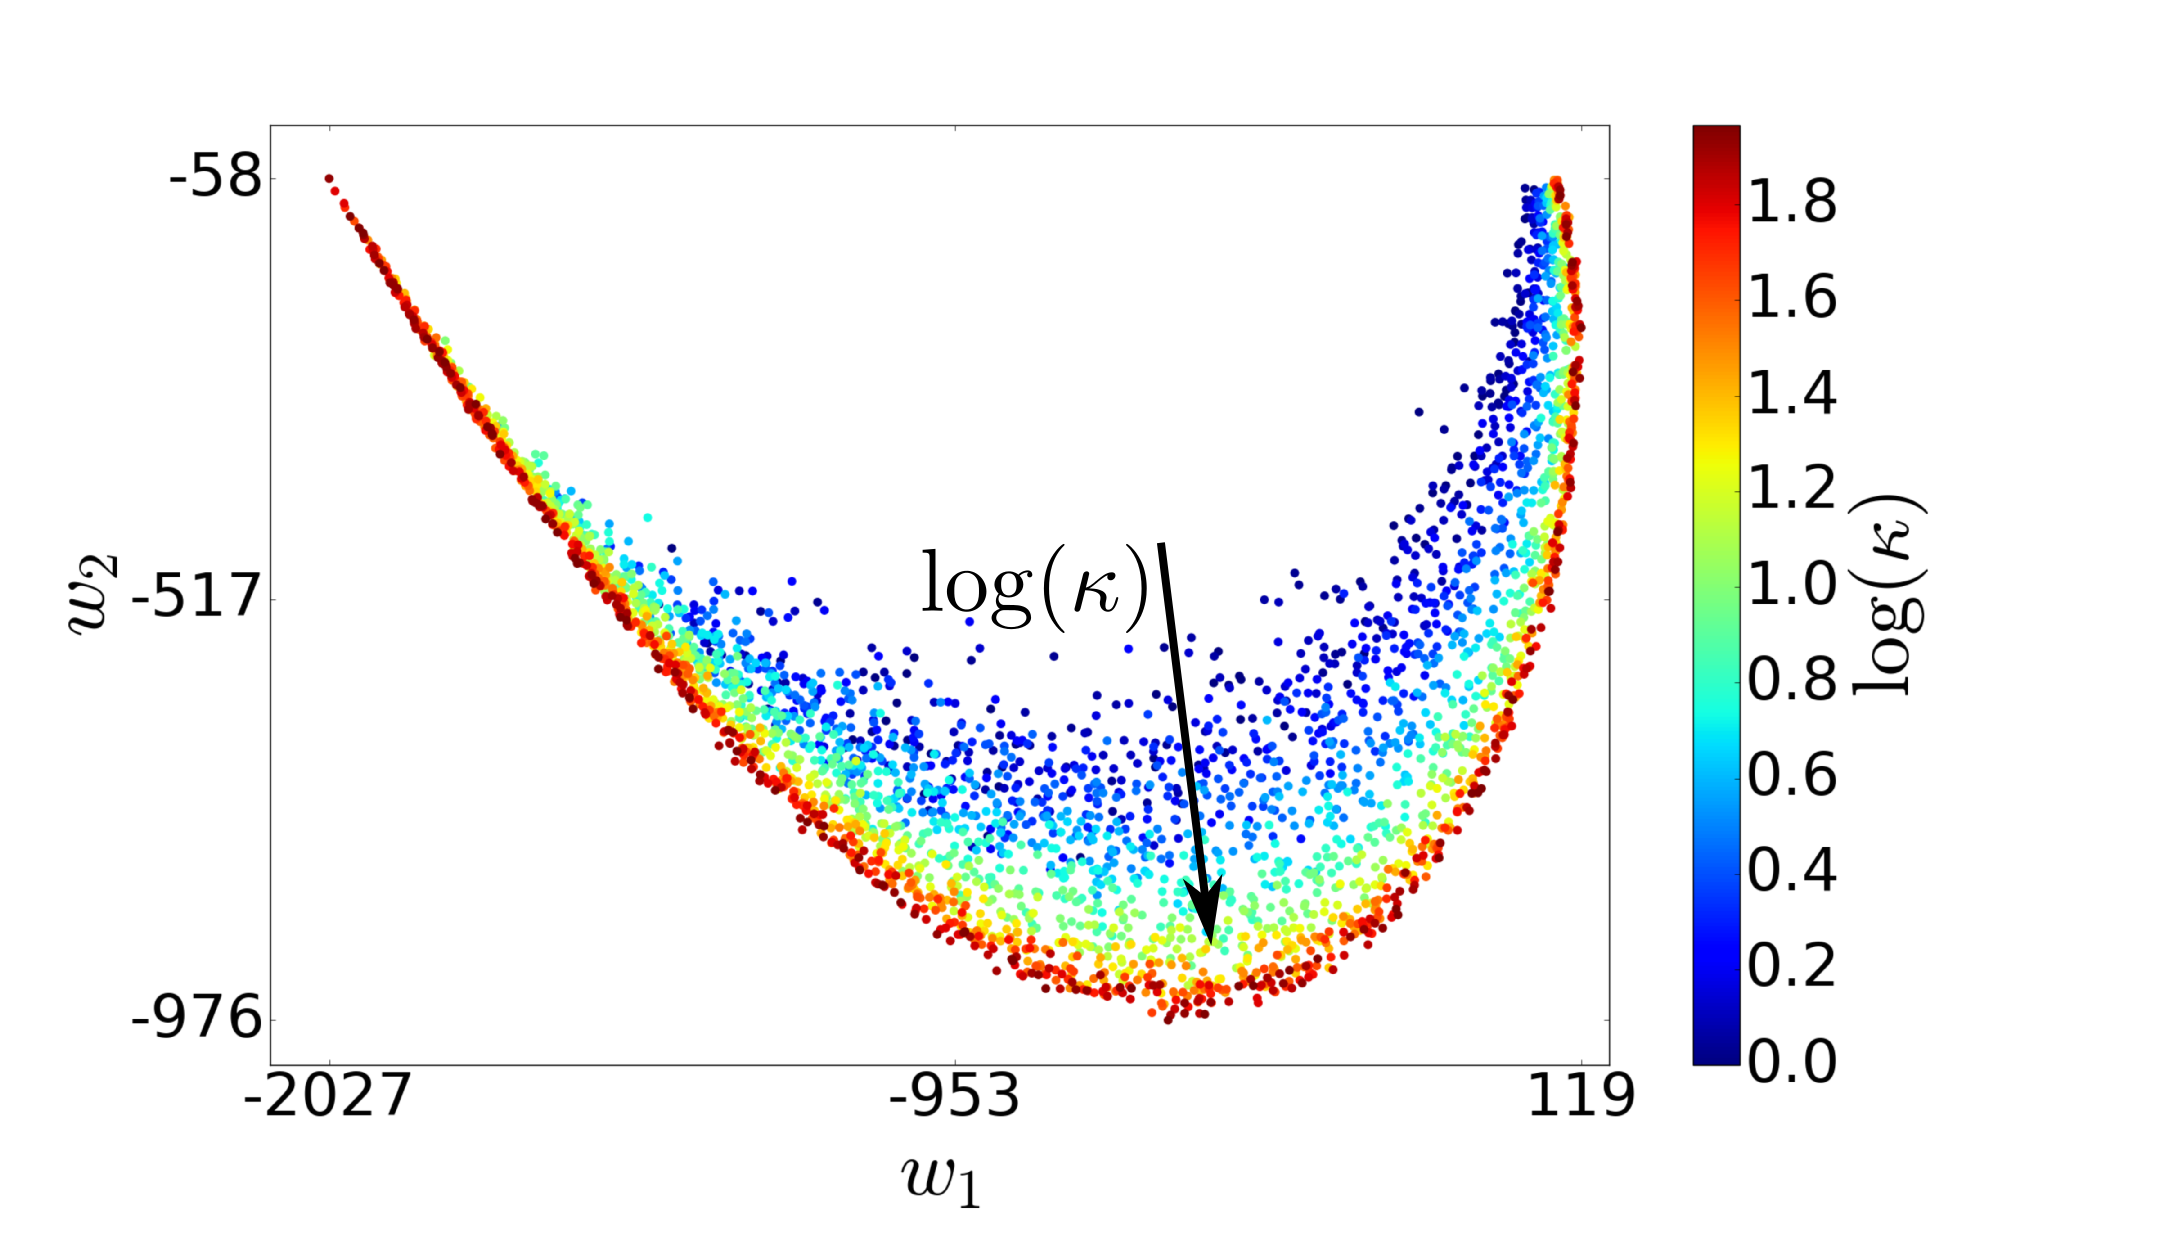
\includegraphics[width=\textwidth]{pca-2d-kappa-a}
      \subcaption{\label{fig:pca-kappa}}
    \end{subfigure}%
    \caption[Principal component analysis of motif-based
    embeddings]{PCA of motif-based embeddings: (a) coloring the
      two-dimensional PCA embedding with $\rho$ and (b) coloring the
      two-dimensional PCA embedding with $\kappa$. \label{fig:pca}}
  \end{figure}

  \subsection{Diffusion Maps}

  Unlike PCA, DMAPS uncovers parameterizations of nonlinear manifolds
  hidden in the data.
  % 
  This is achieved by solving for the discrete equivalent of the
  eigenfunctions and eigenvalues of the Laplace-Beltrami operator over
  the manifold, which amounts to calculating leading
  eigenvector/eigenvalue pairs of a Markov matrix $A$ describing a
  diffusion process on the dataset.
  % 
  As the eigenfunctions of the Laplace-Beltrami operator provide
  parameterizations of the underlying domain, the output eigenvectors
  $\Phi_i$ from DMAPS similarly reveal and parameterize any hidden
  nonlinear structure in the input dataset. The $k$-dimensional DMAP
  of point $x_i$ is given by

  \begin{align*}
    \Psi(x_i; t) = \begin{bmatrix} \lambda_1^t \Phi_1(i) \\ \lambda_2^t
      \Phi_2(i) \\ \vdots \\
      \lambda_k^t \Phi_k(i) \end{bmatrix}
  \end{align*}

  \noindent where $\lambda_i$ is the $i^{th}$ eigenvalue of the Markov
  matrix $A$, $\Phi_i(j)$ the $j^{th}$ entry of eigenvector $i$, and
  the parameter $t$ allows one to probe multiscale features in the
  dataset. See \cite{coifman_diffusion_2006,nadler_diffusion_2006} for
  further details.

  First we applied DMAPS to the dataset described in
  Sec. (\ref{sec:pca}).
  % 
  Given the apparent success of PCA in this setting, one would expect
  DMAPS to also uncover the two-dimensional embedding corresponding to
  different values of $m$ and $\kappa$.
  % 
  Fig. (\ref{fig:dmaps-rk}) shows that this is indeed the case: using
  $\Phi_1$ and $\Phi_4$ to embed the graphs produces a two-dimensional
  surface along which both $\rho$ and $\kappa$ vary independently.

  Additionally, we were interested in embeddings of different model
  trajectories.
  % 
  This dataset was generated by sampling two different model
  simulations as they evolved ($N=2000$ points were sampled from each
  trajectory).
  % 
  The parameters $n$, $m$ and $\kappa$ were held constant at $200$,
  $20100$ and $1.0$ respectively, but one graph was initialized as an
  Erd\H{o}s-R\'{e}nyi random graph (Fig. (\ref{fig:erdos-init})),
  while the other was initialized as a ``lopsided'' graph
  (Fig. (\ref{fig:lopsided-init})).
  % 
  Every $500$ steps the graph would be recorded till $N$ snapshots
  were taken of each trajectory, for a total of $1000000$ steps.
  % 
  Letting $G_e(t)$ refer to the Erd\H{o}s-R\'{e}nyi-initialized system
  at step $t$, and $G_l(t)$ the lopsided-initialized system, the
  embedding $\gamma$ was used to create points
  $\gamma(G_e(t)) = v_e(t) \in \mathbb{R}^8$ and
  similarly $\gamma(G_l(t)) = v_l(t) \in \mathbb{R}^8$.

  DMAPS was then applied to this set of $2N$ points, and the
  three-dimensional embedding using $\Phi_1$, $\Phi_2$ and $\Phi_3$ is
  shown in Fig. (\ref{fig:dmaps-results}).
  % 
  At first, the two trajectories are mapped to distant regions in
  $\mathbb{R}^3$ due to their different initial conditions.
  % 
  They evolve along different ``regions'' of the embedding, taking two
  distinct trajectories on their approach to the stationary state.
  % 
  Eventually, their embeddings meet as they arrive at this final,
  shared state, each asymptotically along opposite sides of the
  slowest eigenvector of the linearization of the steady state.
  % 
  DMAPS thus proves useful in elucidating both geometric and dynamic
  features of the system as shown in Figs. (\ref{fig:dmaps-rk}) and (\ref{fig:dmaps-results}).

  We see that both PCA and DMAPS, when combined with a suitable
  embedding of each graph, can help uncover useful information
  pertaining to the underlying dimensionality of the problem dynamics.


  \begin{figure}
    \vspace{-5mm} \centering
    \begin{subfigure}{0.49\textwidth}
      \centering
      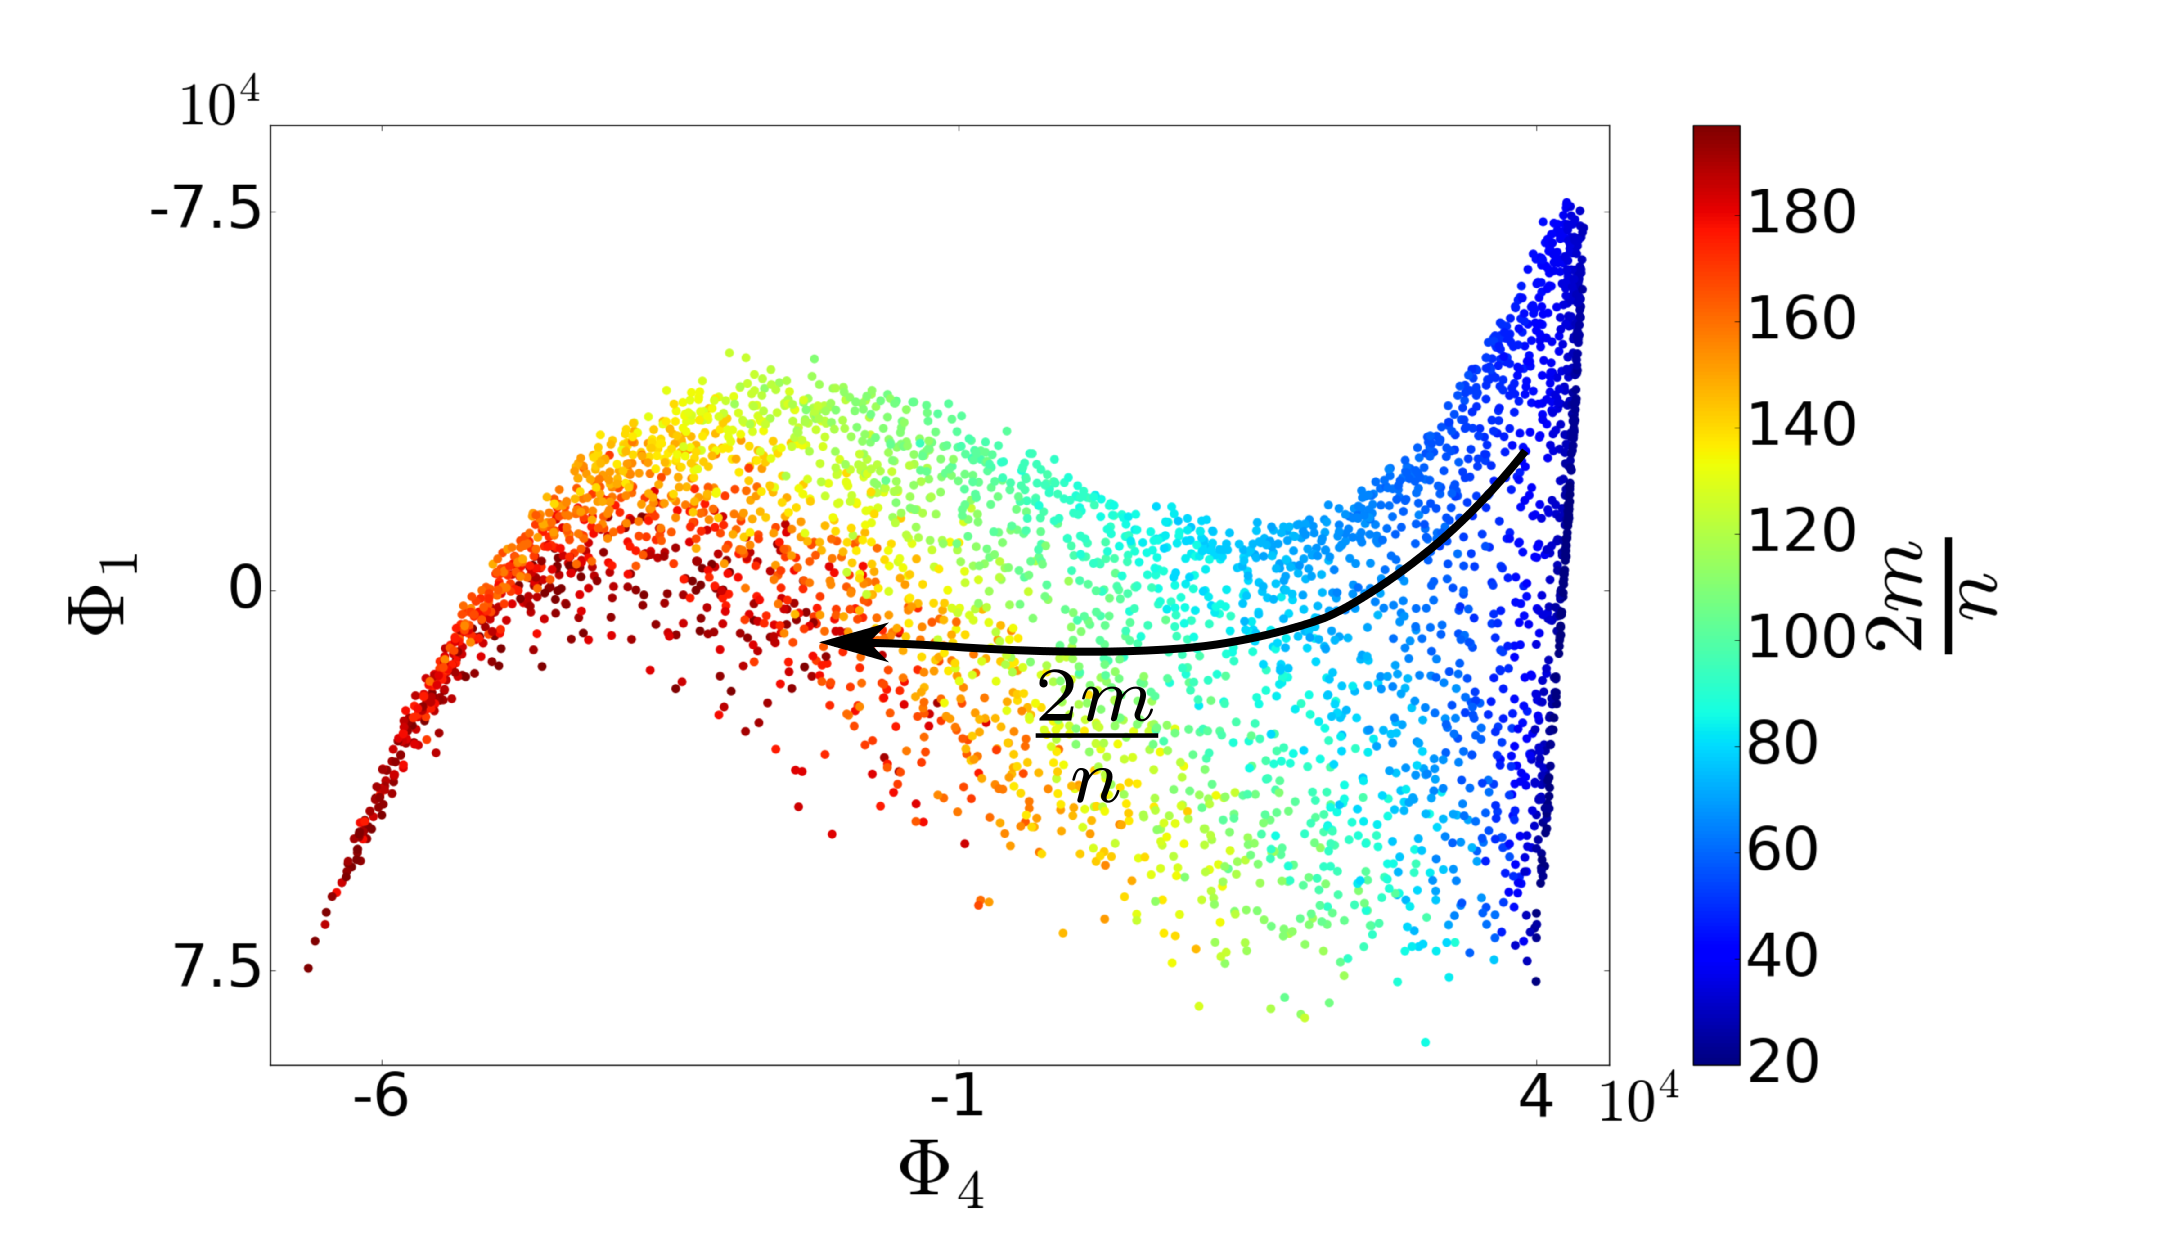
\includegraphics[width=\textwidth]{dmaps-2d-rho-a}
      \subcaption{\label{fig:dmaps-rho}}
    \end{subfigure} %
    \begin{subfigure}{0.49\textwidth}
      \centering
      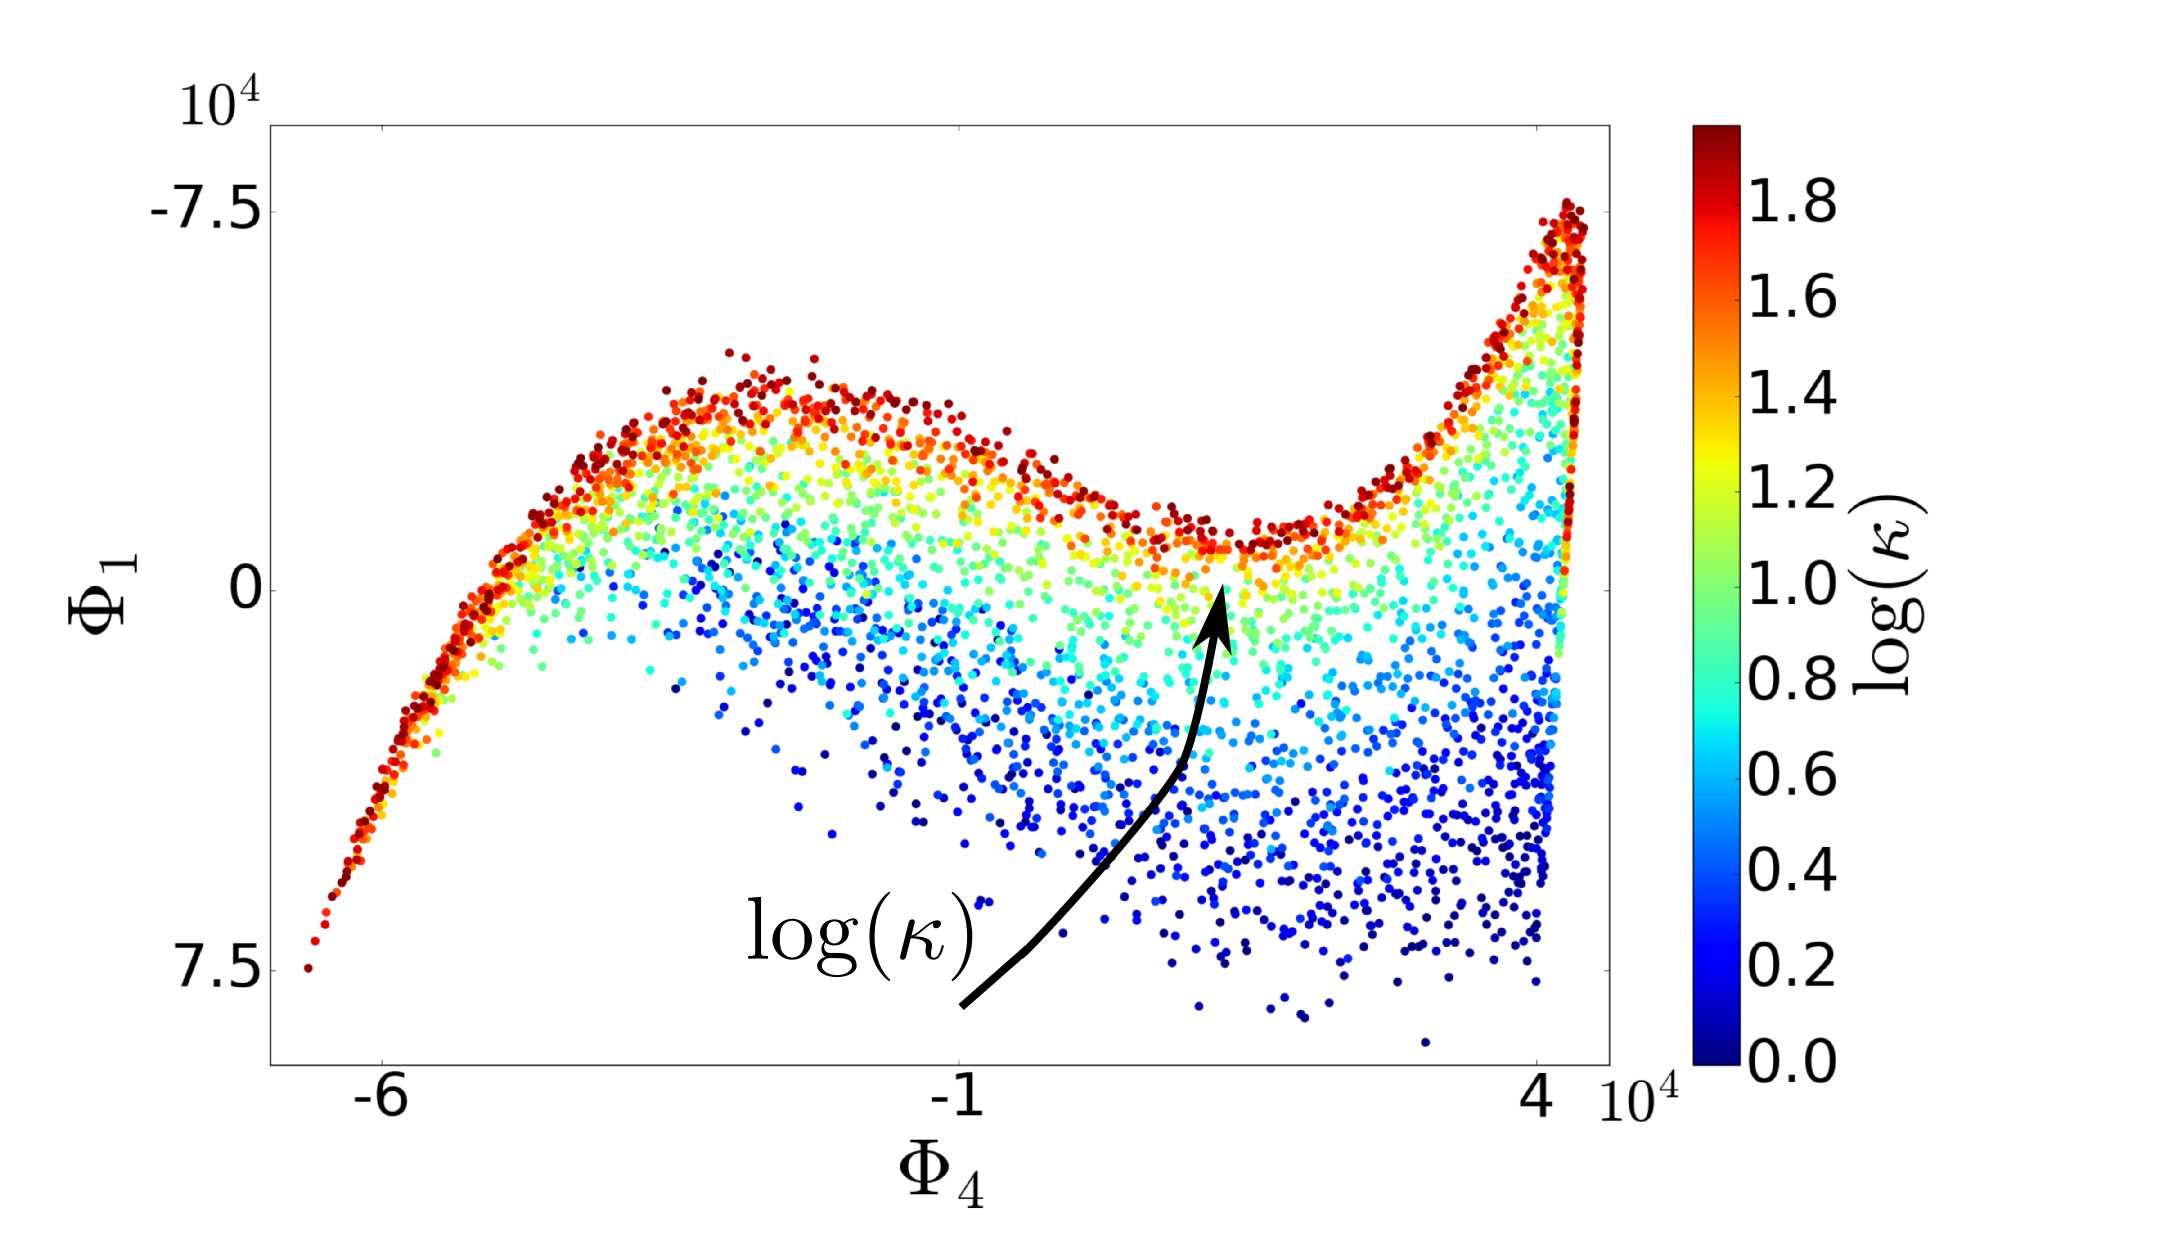
\includegraphics[width=\textwidth]{dmaps-2d-kappa-a}
      \subcaption{\label{fig:dmaps-kappa}}
    \end{subfigure}%
    \caption[DMAP of motif-based embeddings when system parameters are
    varied]{DMAP of motif-based embeddings from a collection of
      simulations run at different parameter values: (a) coloring the
      two-dimensional DMAPS embedding with $\rho$ and (b) coloring the
      two-dimensional DMAPS embedding with $\kappa$. As with PCA,
      DMAPS uncovered the parameters governing the stationary state,
      known from \cite{rath_time_2012} \label{fig:dmaps-rk}}
  \end{figure}

  \begin{figure}
    \vspace{-5mm} \centering
    \begin{subfigure}{0.49\textwidth}
      \centering
      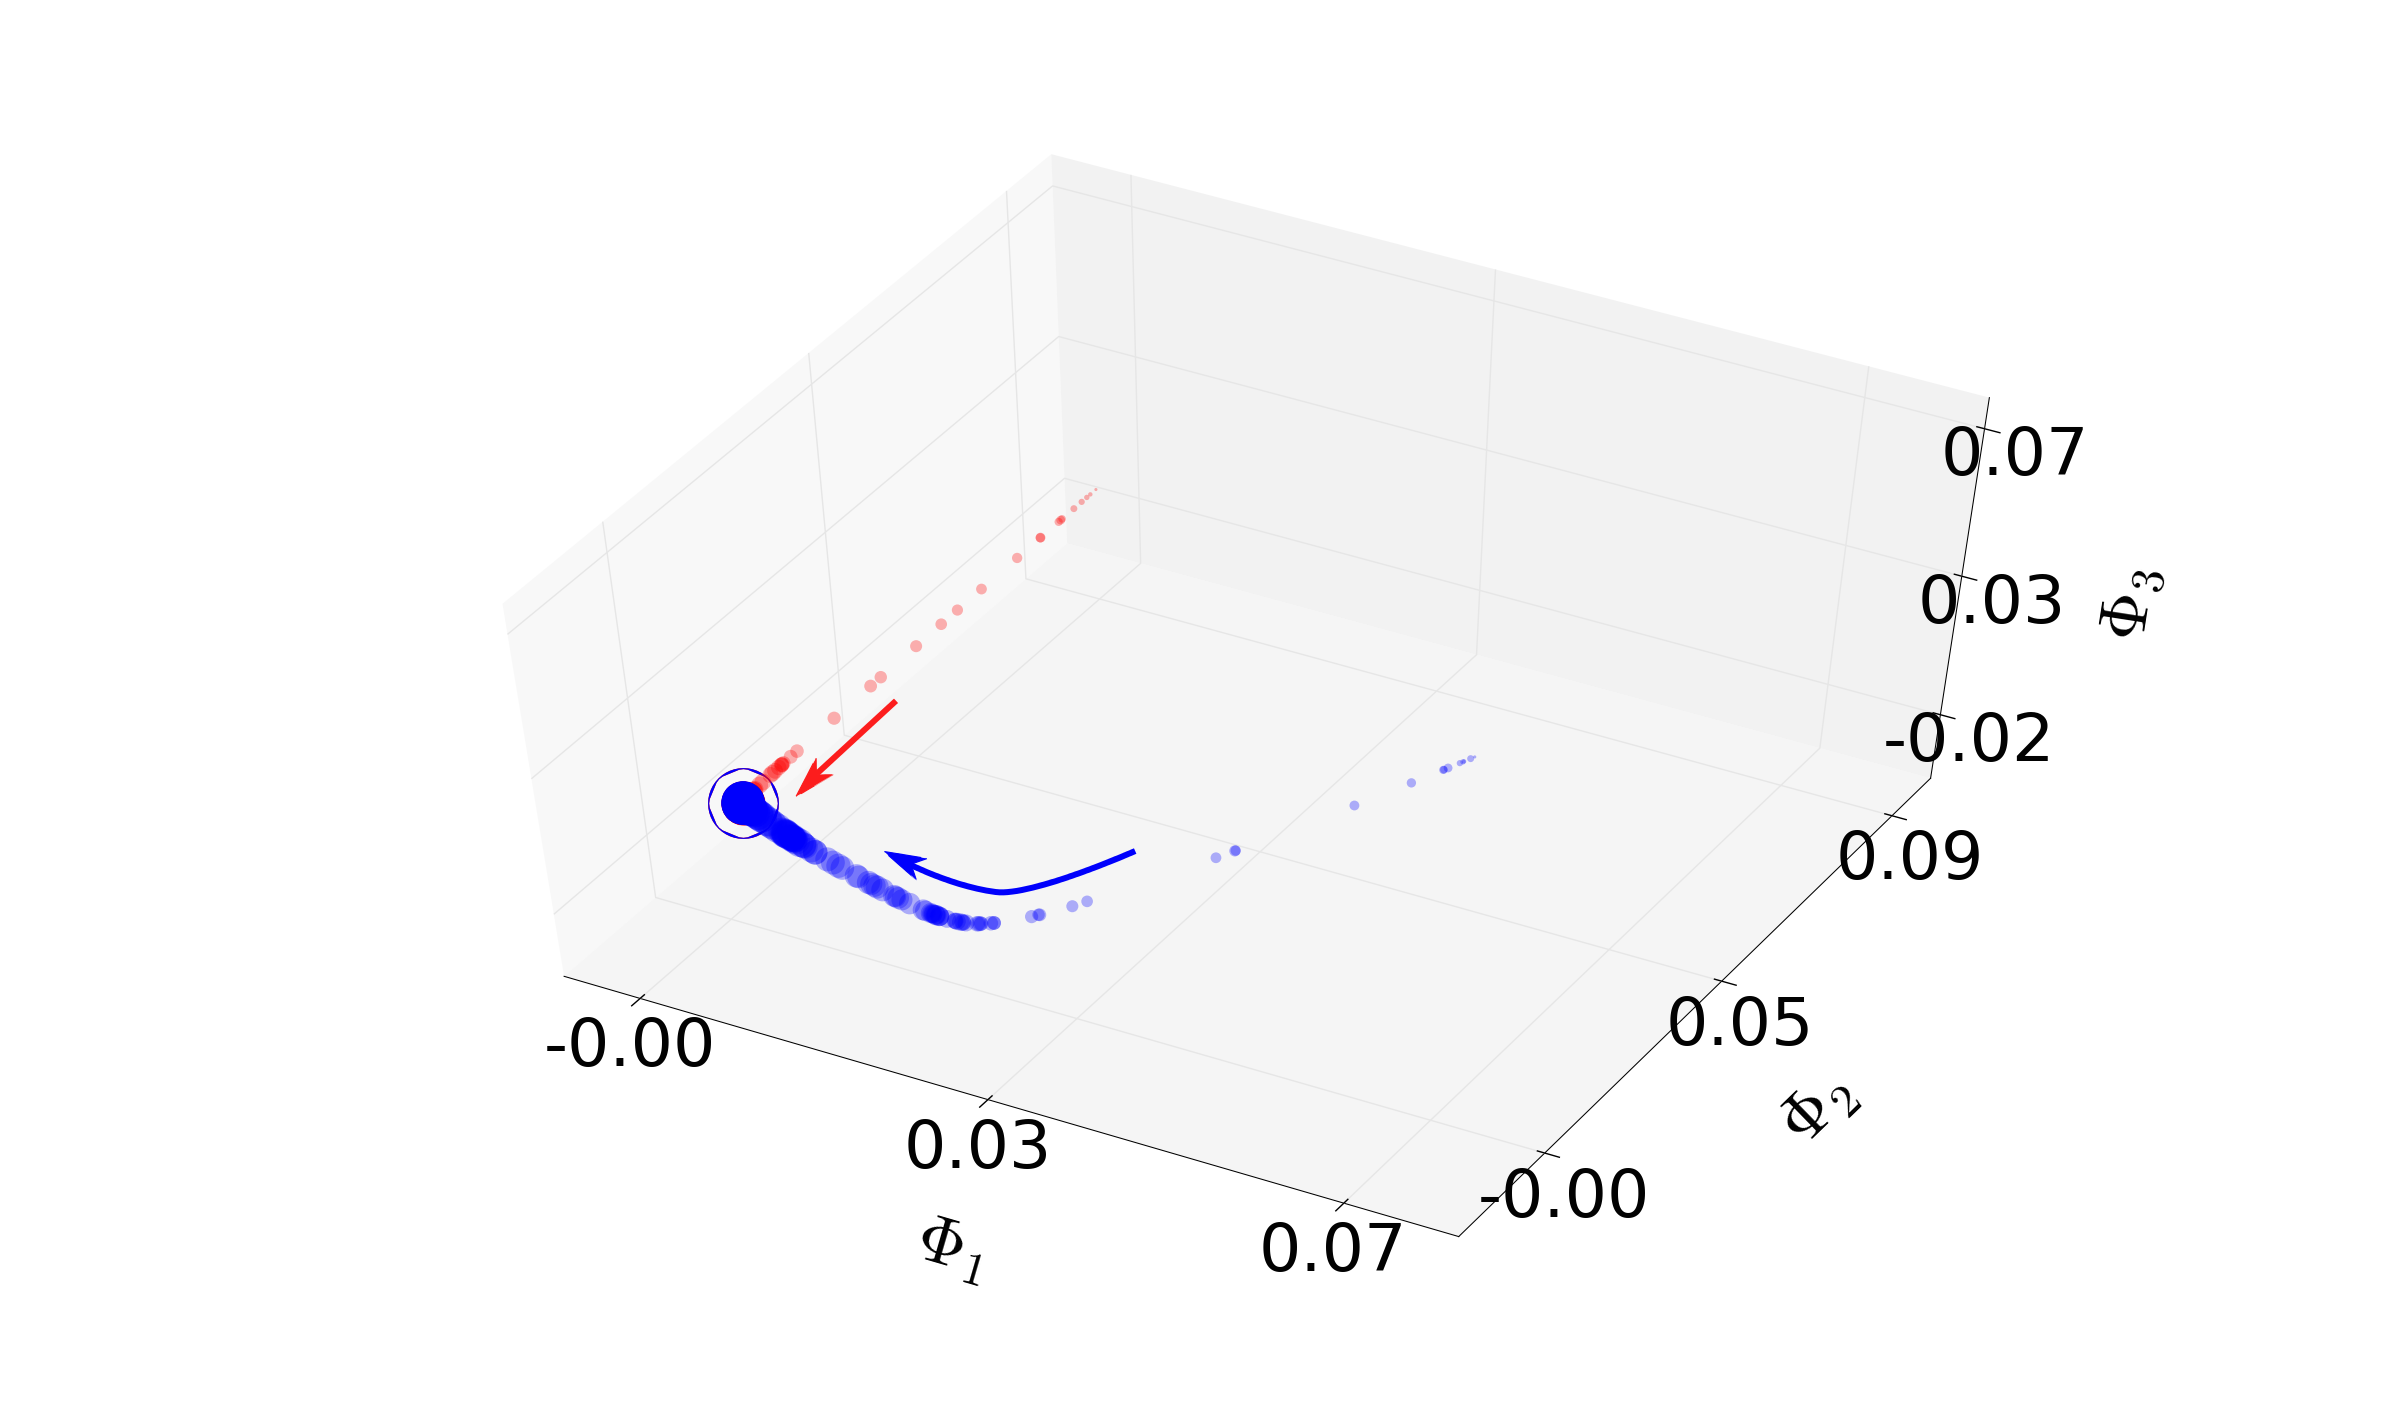
\includegraphics[width=\textwidth]{dmaps-3d-convergence-a}
      \subcaption{\label{fig:dmaps-results-regular}}
    \end{subfigure} %
    \begin{subfigure}{0.49\textwidth}
      \centering
      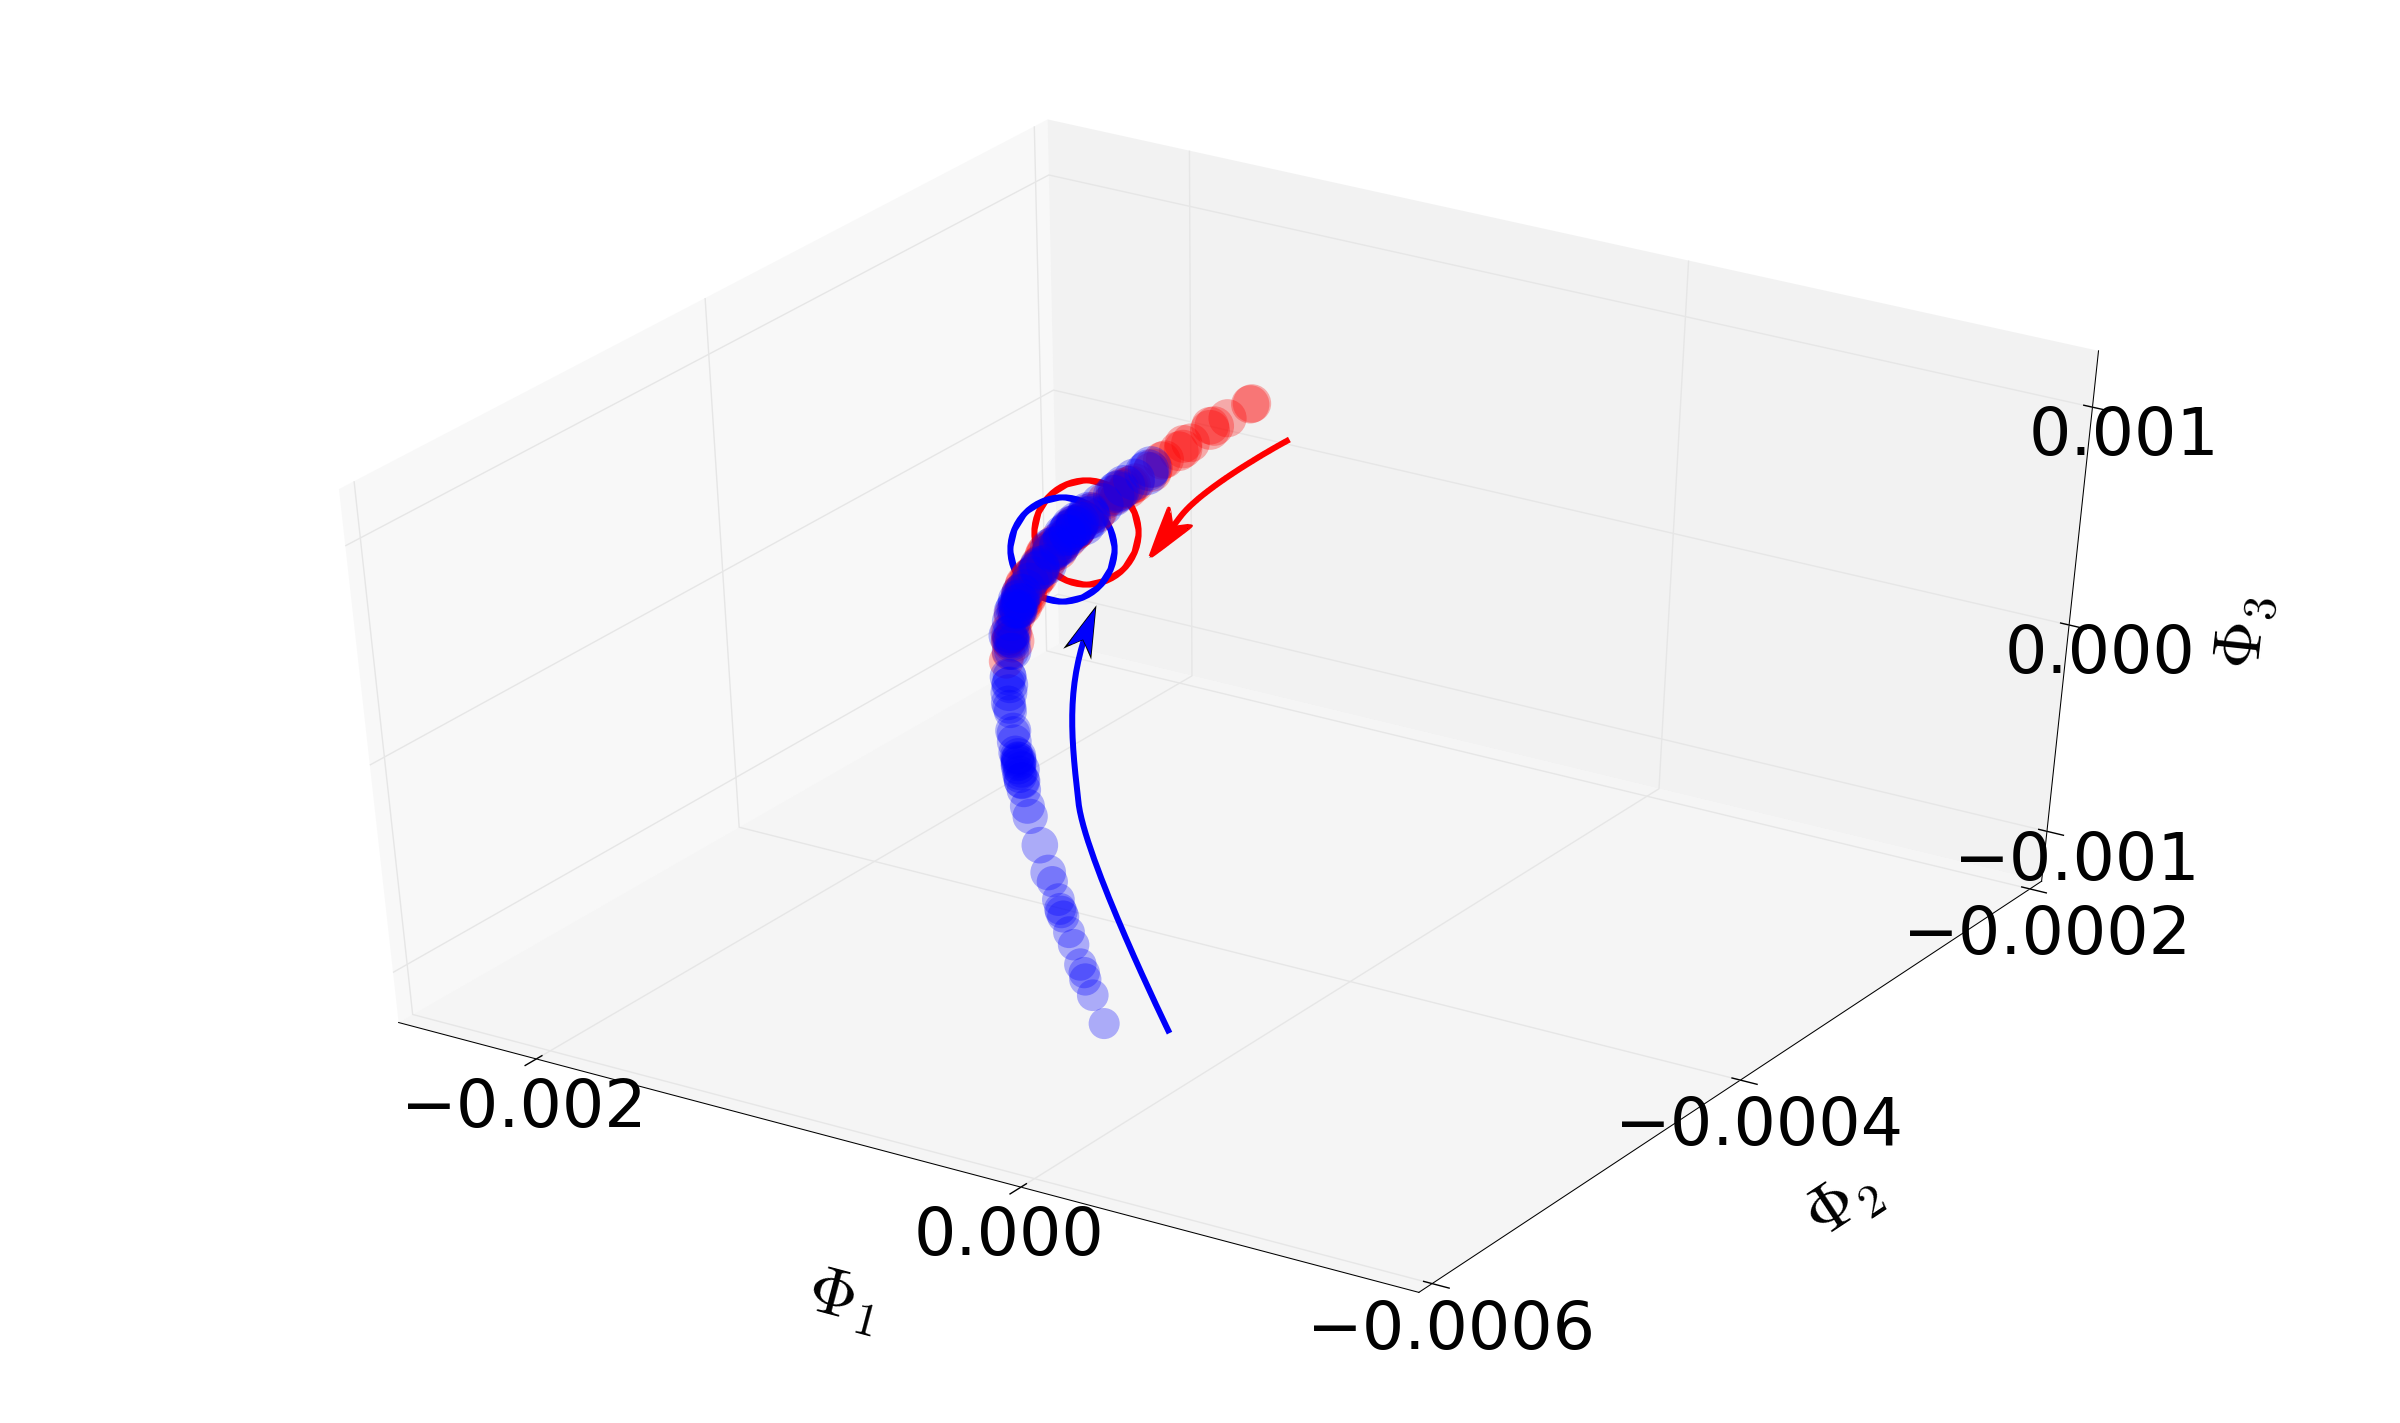
\includegraphics[width=\textwidth]{dmaps-3d-convergence-zoom-a}
      \subcaption{\label{fig:dmaps-results-zoom}}
    \end{subfigure}%
    \caption[DMAP of motif-based embeddings when two trajectories are
    sampled]{DMAP of motif-based embeddings from two separate
      simulation trajectories: (a) embedding of two trajectories
      starting from different initial conditions. While the
      trajectories are initially mapped to separate regions of
      ``embedding space'', they eventually evolve to the same coarse
      stationary state.  Final states are circled, and point size
      grows as more steps are taken in each trajectory.  (b) Enlarged
      view of the final points in the previous plot, revealing the
      approach to a similar final state along opposite sides of the
      slowest eigenvector of its linearization.  Here, the average of
      the final fifty points is circled. Due to the stochastic nature
      of the system, the final embeddings mildly fluctuate randomly
      about the shared stationary state. \label{fig:dmaps-results}}
  \end{figure}

  \section{Conclusion}

  The equation free framework was successfully applied to the
  edge-conservative preferential attachment model, accelerating
  simulations through CPI and locating stationary states through
  coarse Newton-GMRES. This indicates potential avenues for improving
  simulation times of other complex network models, such as those
  found in epidemiology.
  % 
  Additionally, an underlying two-dimensional description was
  uncovered via PCA and DMAPS. These automated methods of
  dimensionality-reduction are quite general, and can in principle be
  applied in a wide range of network settings to probe hidden
  low-dimensional structure. For an application in the setting of
  labeled nodes, see ({\cite{kattis_modeling_2016}}).

  However, an open area of investigation is the interpretation of the
  output from the PCA and DMAPS techniques.
  % 
  As a linear map, PCA retains a clear relationship between its input
  and output, but is less effective when data lie on highly nonlinear
  manifolds.
  % 
  DMAPS may perform better the task of dimensionality reduction, but
  it is unclear how the embedding coordinates relate to physical
  features of the sampled networks.
  % 
  While this approach opens several promising avenues in
  coarse-graining complex network dynamics, it also reveals two
  ``bottlenecks'' for the process: (a) the selection of informative
  and practically computable graph distance metrics, necessary in the
  discovery of good coarse variables; and (b) the construction of
  network realizations consistent with (conditioned on) specific
  values of collective observables.
  % 
  Both items are, and we expect will continue being, the subject of
  intense investigation by many research groups, including ours.

\chapter{Dimensionality reduction of network epidemiology
  model \label{ch:sis}}
% Abstract The exploration of epidemic dynamics on dynamically
% evolving (“adaptive”) networks poses nontrivial challenges to the
% modeler, such as the determination of a small number of informative
% statistics of the detailed network state (that is, a few “good
% observables”) that usefully summarize the overall (macroscopic,
% systems level) behavior. Trying to obtain reduced, small size
% accurate models in terms of these few statistical observables – that
% is, coarse-graining the full network epidemic model to a small but
% useful macroscopic one – is even more daunting. Here we describe a
% data-based approach to solving the first challenge: the detection of
% a few informative collective observables of the detailed epidemic
% dynamics. This will be accomplished through Diffusion Maps, a
% recently developed data-mining technique. We illustrate the approach
% through simulations of a simple mathematical model of epidemics on a
% network: a model known to exhibit complex temporal dynamics. We will
% discuss potential extensions of the approach, as well as possible
% shortcomings.

\section{Introduction}

Mathematical modeling of epidemic dynamics is an indispensable tool in
understanding and mitigating the spreading of disease in the real
world
\cite{gross_epidemic_2006,pastor-satorras_epidemic_2015,segbroeck_adaptive_2010,zhou_epidemic_2012}.
As computational power, numerical simulation techniques and, most
recently, “big data” tools and techniques progress, the degree of
realism in these mathematical models constantly improves. From simple
nonlinear models of Susceptible-Infected-Recovered (SIR) or
Susceptible-Infected-Susceptible (SIS) dynamics that are based on
spatial averaging (so called mean-field models, consisting of a few
nonlinear Ordinary Differential Equations (ODEs)) we have graduated to
models with detailed spatial information and structure, incorporating
not only geographical details of communities and cities but also
information about the social interactions between the individuals
involved
\cite{colizza_modeling_2006,wang_epidemic_2011,eubank_modelling_2004}.
From mean field ODEs the models now become large-scale, stochastic,
individual-based simulations on networks (geographical as well as
social).  While this framework is convenient for investigating many
different initial conditions combined with many different network
connectivities and many different interaction/evolution rules,
recording and rationalizing a useful summary of the dynamics (the
relevant macroscopic, systems-level statistics of these scenarios) is
crucial for systems-level understanding and control. Finding the right
macroscopic observables for such detailed simulations, the right
variables, to summarize the epidemic dynamics is still a daunting
task.

Over the last decade our group has proposed and developed the
so-called Equation-Free computational framework for complex/multiscale
systems modeling: given a detailed (here, individual/agent-based)
simulation algorithm, this framework enables the study of
coarse-grained, systems level dynamics through the design, execution
and processing of the brief bursts of fine scale simulation data;
Equation-Free algorithms like Coarse Projective Integration (CPI) take
the form of “wrappers” around the fine scale code (say, an agent-based
epidemic simulation code on an adaptive network)
\cite{gear_equation-free_2003,kevrekidis_equation-free:_2004,tsoumanis_coarse-graining_2012,siettos_equation-free_2011}. Yet
for this approach to be successful, one needs to a priori know what
the right macroscopic statistics are (e.g., the right few leading
moments of the distribution of susceptible or of infected individuals
in the population) in terms of which the epidemic statistics can be
informatively summarized.

This paper considers the case where such informative and parsimonious
system-level statistics are not a priori known.  In this case the
Equation-Free modeling approach can still be carried through, as long
as the right macroscopic variables can be discovered through the
mining of (big) computational simulation data. This is a
“doubly-data-based” modeling strategy: using data produced from
detailed, individual level, fine scale simulation bursts to detect the
number and identity of the macroscopic observables; and then, armed
with this knowledge, design and execute new, informative, microscale
simulations to systematically explore the evolution of the
epidemic. This jointly “equation-free, variable-free” approach holds
great promise for accurate, fast and informative systems-level
simulation of detailed, realistic epidemic models – the “right
observables” come from the (previously computed) data, as does the
design of “the right simulations” to obtain useful new information.


When the state of the fine-scale model at a given moment in time can
be mathematically described as a (long) vector in $\mathbb{R}^n$
(e.g. the state of a large number of agents), both linear data-mining
techniques, such as Principal Component Analysis (PCA), as well as
nonlinear data-mining techniques such as ISOMAP or Diffusion Maps
(DMAPS) can be applied to simulation data ensembles to obtain “the
right” macroscopic observables
\cite{jolliffe_principal_2014,coifman_diffusion_2006,tenenbaum_global_2000}. But
when the data involve evolving graphs (in our case, we are interested
in epidemic dynamics on adaptively evolving networks), finding good
macroscopic observables based on simulation databases is a nontrivial
task. We present a simple modification/extension of the DMAPS
procedure that allows us to detect the (small) number of these
observables for epidemics on adaptive networks based on data mining
only.  The “macro-variables” discovered by this process for the case
of a SIS epidemic on an adaptive network will be presented, discussed,
and contrasted to traditionally used macro-variables for the same
problem.

Our approach is motivated by, and illustrated through, SIS dynamics on
adaptive networks
\cite{gross_epidemic_2006,gross_adaptive_2008,gross_robust_2008}. The
computational methodology, however, is in principle applicable to many
problems that involve the dynamic evolution of networks with both
labeled nodes (when we know the identity of individuals) or unlabeled
nodes (when we do not)
\cite{sayama_modeling_2013,huepe_adaptive-network_2011}. We link the
DMAPS procedure with quantities that allow us to usefully compare
different networks; we use this approach to detect the number of
macroscopic observables involved in the dynamics of our SIS epidemic
model, and compare these data-based observables with typical network
statistics. The last few years have seen several innovative approaches
to finding accurate reduced models for dynamic, network-evolution
problems, extending and complementing well-established techniques like
those based on moment closures \cite{gross_robust_2008}. Our approach
should be considered as a data-mining based alternative to these
techniques with the advantages of not requiring any knowledge about
the underlying model and automating the process of feature extraction.

The rest of the paper is organized as follows: We will first describe
our implementation of a SIS epidemic model on an adaptive network,
from which the simulation data will be obtained. We then briefly
discuss established linear (PCA) and nonlinear (DMAPS) data mining
techniques. We then present an extension to DMAPS that expands their
applicability to data in the form of evolving networks (where the
connectivity of the network evolves in time along with the state of
the network nodes). We first validate our network data mining approach
on data obtained from a simple Watts-Strogatz network model
\cite{watts_collective_1998}. We then present our main results: the
application of our data-mining technique to data collected from
dynamic SIS simulations on an adaptive network, obtained over a range
of epidemic parameter values where it is known that complex,
oscillatory dynamics arise. We discuss the relation of the variables
detected through our approach to those of more traditional,
moment-based approaches, and conclude with a brief perspective on
potential shortcomings but also potential fruitful applications of the
approach.

\section{The adaptive SIS model}

An implementation of the adaptive SIS model can be constructed by
considering a labeled graph $G$ with $N$ nodes and $L$ links, with
each node representing an individual in a social network; the state of
each individual, either susceptible (S) or infected (I), constitutes
the node label. Edges between individuals are defined as SS-links,
II-links, or SI-links, according to the label of the nodes they
connect. Starting with a given initial network connectivity pattern (a
given network topology), the evolution of the model can be
characterized by three substeps, which together constitute a time step
in the model's evolution:

\begin{enumerate}
  \item All infected nodes recover with
    probability $r$, becoming susceptible.
  \item For every SI-link, the
    susceptible individual becomes infected with probability $p$.
  \item Every SI-link is removed with probability $w = w_0 \rho$. In this case, a
    new edge between the corresponding susceptible node and another
    susceptible node is formed. The new link is made with a node
    chosen uniformly at random from the set of all other susceptible
    individuals.
\end{enumerate}

The probability of rewiring $w = w_0 \rho$ is based on a constant
input parameter $w_0$ and the infected fraction $\rho = i/N$, where
$i$ is the number of infected nodes. These rules are motivated by the
assumption that humans are more likely to avoid infected individuals
proportionally to their awareness of disease spread, which here is
assumed to be directly proportional to the infected fraction of the
population \cite{gross_epidemic_2006}. Figure~\ref{fig:sis2} shows a
schematic of this evolution process, while Figure~\ref{fig:sis1} gives
a sense of the model behavior in different parameter regimes.

Although the behavior of this model is inherently complex (see the
bifurcation diagram in Figure~\ref{fig:sis1}, reproduced by
permission) \cite{gross_robust_2008}, it has been previously
established that the system-level dynamics of a sufficiently large
network can be captured by just three macroscopic observables: the
number of infected nodes $i$, the number of SS-links $l_{SS}$ and the
number of II-links $l_{II}$ . These variables suffice to describe all
long-term dynamical behavior exhibited by the system, since the values
of other variables (higher order moments of the network state) quickly
become slaved to (functions of) these three and do not contribute
extra degrees of freedom over long timescales. As the infection
parameter $p$ varies, one can observe stationary states as well as
coarsely oscillatory dynamics, and even coexistence between the two
(associated with an apparent subcritical coarse Hopf bifurcation)
\cite{holmes_turbulence_2012}.  In this paper we will show how to
extract the relevant observables responsible for the dynamics of the
system without making use of any prior knowledge about their
suitability. This will be accomplished by first constructing a
suitable similarity measure for quantifying graph differences, and
secondly, by applying DMAPS on ensembles of graphs resulting from the
dynamic simulation of the model’s evolution.

\begin{figure}[!htp]
\centering
\begin{tabular}{cc}
  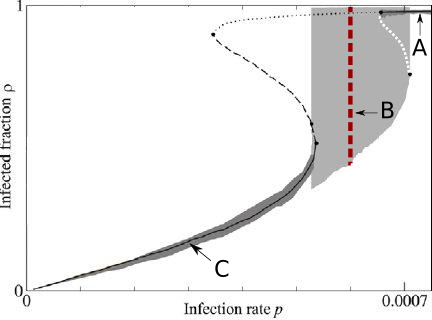
\includegraphics[width=0.45\textwidth]{1a} &
  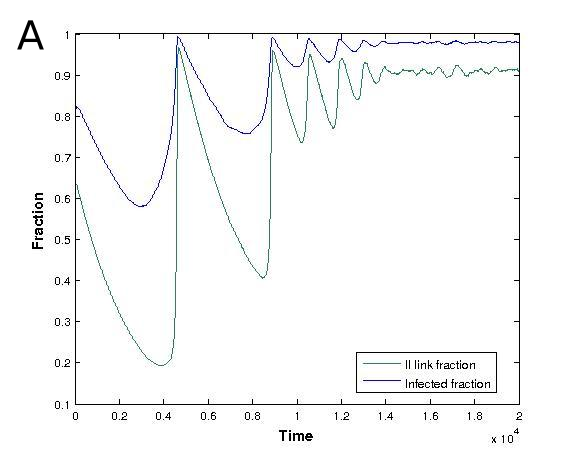
\includegraphics[width=0.45\textwidth]{1b}\\
  (a) & (b)\\
  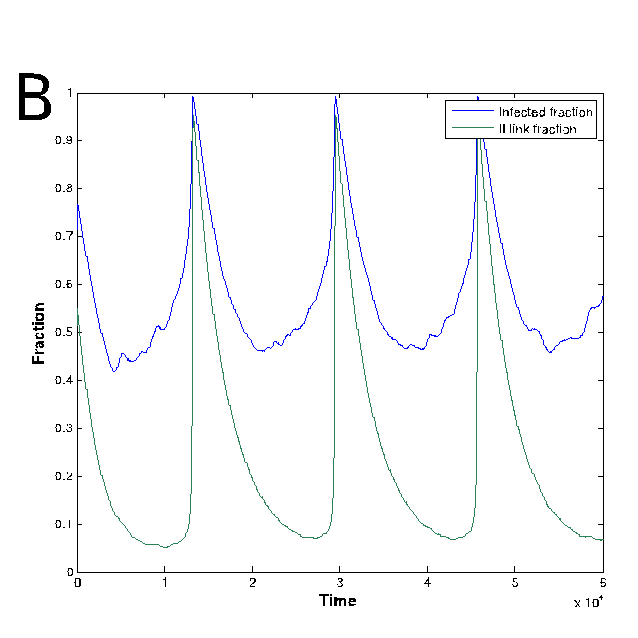
\includegraphics[width=0.45\textwidth]{1c} &
  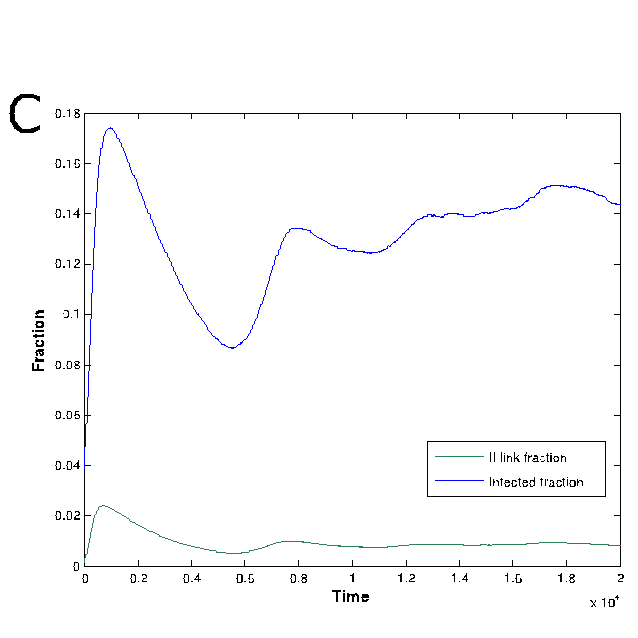
\includegraphics[width=0.45\textwidth]{1d}\\
  (c) & (d) \\
  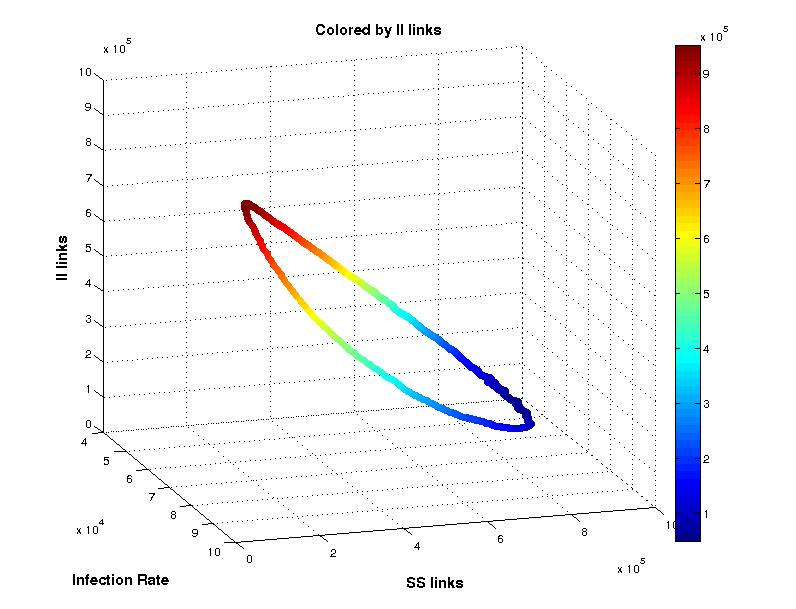
\includegraphics[width=0.45\textwidth]{1e} &
  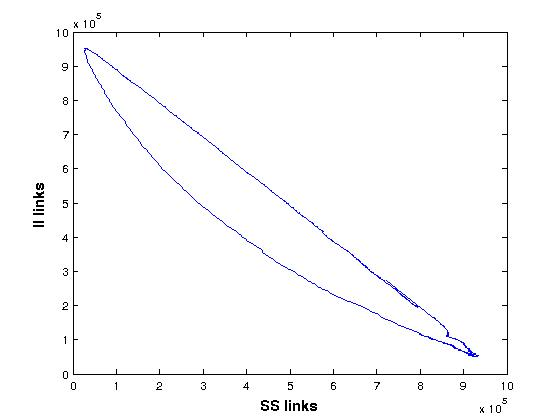
\includegraphics[width=0.45\textwidth]{1f}\\
  (e) & (f)
\end{tabular}
\caption[Quantitative behavior of SIS model]{(a) Model bifurcation diagrams wrt. the infection rate
  parameter $p$ (reprinted with permission)
  \cite{gross_epidemic_2006}. (b) The system evolves to a stable
  stationary state for $p = 0.00073$. (c) Oscillatory behavior
  indicating a (coarse) limit cycle at $p = 0.0006$. (d) Stable
  stationary state for $p = 0.0003$. Bottom graphs indicate the
  relationship between $i$, $l_{SS}$ , and $l_{II}$ over the course of
  one complete oscillation for $p = 0.0006$. Model parameters:
  $(r, w_0, N, L) = (0.0002, 0.03, 10^5 , 10^6)$. \label{fig:sis1}}
\end{figure}

\begin{figure}[!htp]
\centering
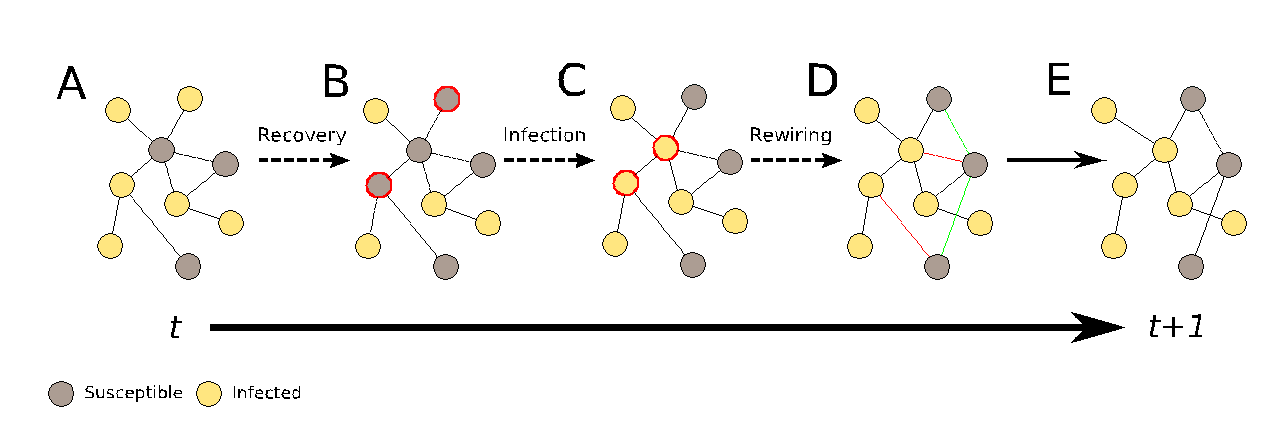
\includegraphics[width=0.9\textwidth]{2}
\caption[Schematic of SIS model evolution]{Schematic of the adaptive SIS model evolution: the three
  substeps constituting one SIS evolution timestep. (A) The initial
  graph at time $t$. (B) Each infected node recovers with probability
  $r$, becoming susceptible. (C) The disease spreads along SI-links
  with probability $p$, infecting susceptible nodes. (D) With
  probability $w$, each SI-link is broken and a new SS-link is
  created. (E) The final graph at $t+1$. Broken links and nodes that
  change status between steps are colored in red, while rewired links
  are colored in green. \label{fig:sis2}}
\end{figure}

\section{A brief discussion of dimensionality reduction}

Analysis of the dynamics of this epidemic model, especially as the
size of the network grows, is hindered by its size and complexity. Not
only are there many nodes to keep track of over thousands of time
steps, but each step is also comprised of a number of different
(stochastic) actions. These factors combine to make systematic
exploration of such a system computationally intractable; one may only
execute and observe many different scenarios computationally
(different initial networks, node states, and parameter
values). Additionally, it is not clear which variables, or indeed even
how many, play a determining role in summarizing long-term system
behavior. This motivates the development of an algorithmic approach to
identifying the crucial features of the system. Not only will these
important features themselves aid in better understanding the problem
and in summarizing its behavior, but they could also be used in an
Equation-Free framework to enable the sort of analysis typically
reserved for simpler systems (e.g. a few mean-field ODEs). Below, we
present our first step towards this goal: the use of the DMAPS data
mining technique to identify the important observables in the SIS
model from simulation datasets.

\section{Principal component analysis and diffusion maps}

Given a dataset ${x_1, x_2, \dots, x_N}$ (with each
$x_i \in \mathbb{R}^n$), several approaches exist to uncover a
lower-dimensional description ${y_1, y_2, \dots, y_N}$ of the data,
where $y_i \in \mathbb{R}^p$ and $p \ll n$. These new
lower-dimensional points $y_i$ accurately capture the salient features
of the original data set, with minimal loss of important
information. In essence, we try to describe our data as concisely as
possible.

Perhaps the best-known method for achieving this is Principal
Component Analysis (PCA) \cite{jolliffe_principal_2014}, detailed in
Section~\ref{sec:pca}. Unfortunately, PCA assumes the data lies on,
or around, a linear subspace, whereas data points generally lie on
nonlinear manifolds. To circumvent this limitation we turn to the
nonlinear dimensionality reduction technique of Diffusion Maps (DMAPS)
\cite{coifman_diffusion_2006}. The algorithm is detailed in
Section~\ref{sec:dmaps}. In brief, by simulating a diffusion process
over the dataset, DMAPS will reveal the underlying low-dimensional
nonlinear structure.

\section{Similarities between different networks}

In order to simulate diffusion over the dataset, DMAPS requires a
scalar distance between two data points, $d(x_i, x_j)$. When each
point is a vector the Euclidean distance between points is often
sufficient. However, in the dataset we investigate below, each point
$x_i$ is not a vector, but actually a graph (or network), which we
represent as $G_i$.

The literature contains a number of ways of quantifying the distance
between two graphs, $d(G_i, G_j)$, for example by measuring how easily
$G_i$ can be transformed into $G_j$ (graph edit distance), or by
comparing random walks on the graphs (spectral distance)
\cite{bunke_graph_1998,gao_survey_2010,papadimitriou_web_2010,vishwanathan_graph_2010}. In
this paper, we consider two graphs to be similar if they share similar
numbers of certain features. More precisely, we define a list of $k$
subgraphs $S = {s_1, s_2, \dots, s_k}$, such as the single edge, the
two connected edges, the triangle shown in Figure~\ref{fig:sis4} etc. Then we
record how many times each subgraph appears in our input graph in a
vector $v_i = {c_1^i, c_2^i, \dots, c_k^i}$, where $c_j^i$ is the
number of times subgraph $s_j$ was found in input graph $G_i$. This
process maps each graph to a vector of subgraph densities, the counts
$G_i \rightarrow v_i, \; v_i = {c_1^i, c_2^i, \dots, c_k^i}$ in
$\mathbb{R}^k$, thus embedding the graph as a point in
$\mathbb{R}^k$. We then use these k-long vectors (k-dimensional
points) as the input to DMAPS, and use the Euclidean distance between
them as our notion of graph similarity. Thus
$d(G_i, G_j) = \| v_i - v_j \|_2$. Figure~\ref{fig:sis4} presents a schematic
illustrating this subgraph-enumeration process.


In the SIS model, we are actually working with labeled graphs, since
each node has one of two labels – susceptible (S) or infected (I). It
is inappropriate to simply ignore network labels, since networks with
the same connectivity, but with different node labels, can behave in
extremely different ways and should thus be considered dissimilar. To
overcome this issue, for a given labeled graph $G$ we choose to
consider three separate unlabeled subgraphs $G_0, G_S$ and $G_I$. Here
$G_0$ is the initial graph $G$ without node labels and $G_S$, $G_I$
the unlabeled subgraphs obtained (induced) by only considering the S,
or the I nodes respectively. We will represent each overall labeled
graph by the concatenation of the three count vectors $v_0, v_I, v_S$
into $v = [v_0 v_I v_S]^T$, again using the Euclidean norm to quantify (dis)similarity
between them. Note that we scale the subgraph counts so that we really
measure a “density” of $s$ in $G$, given by:

\begin{align}
  \label{eqn:homdenG}
  \rho(H,G) := \frac{1}{{n\choose k}} \!  \sum_{\varphi:[k] \to [n]} \!
  \left[ \forall  i, j \in [k] \! : \! H(i,j) \! = \! G(\varphi(i),
  \varphi(j)) \right].
\end{align}

where $n$ is the number of nodes in $G$, $k$ is the number of nodes in
$s$, $\varphi$ is an injection from the first $k$ integers to the
first $n$, and $\!$ is an indicator function which takes the value 1
when subgraph $s$ has been located in $G$. The subgraph enumeration
procedure in the case of labeled nodes is illustrated in Figure~\ref{fig:sis5}.

\begin{figure}[!htp]
\centering
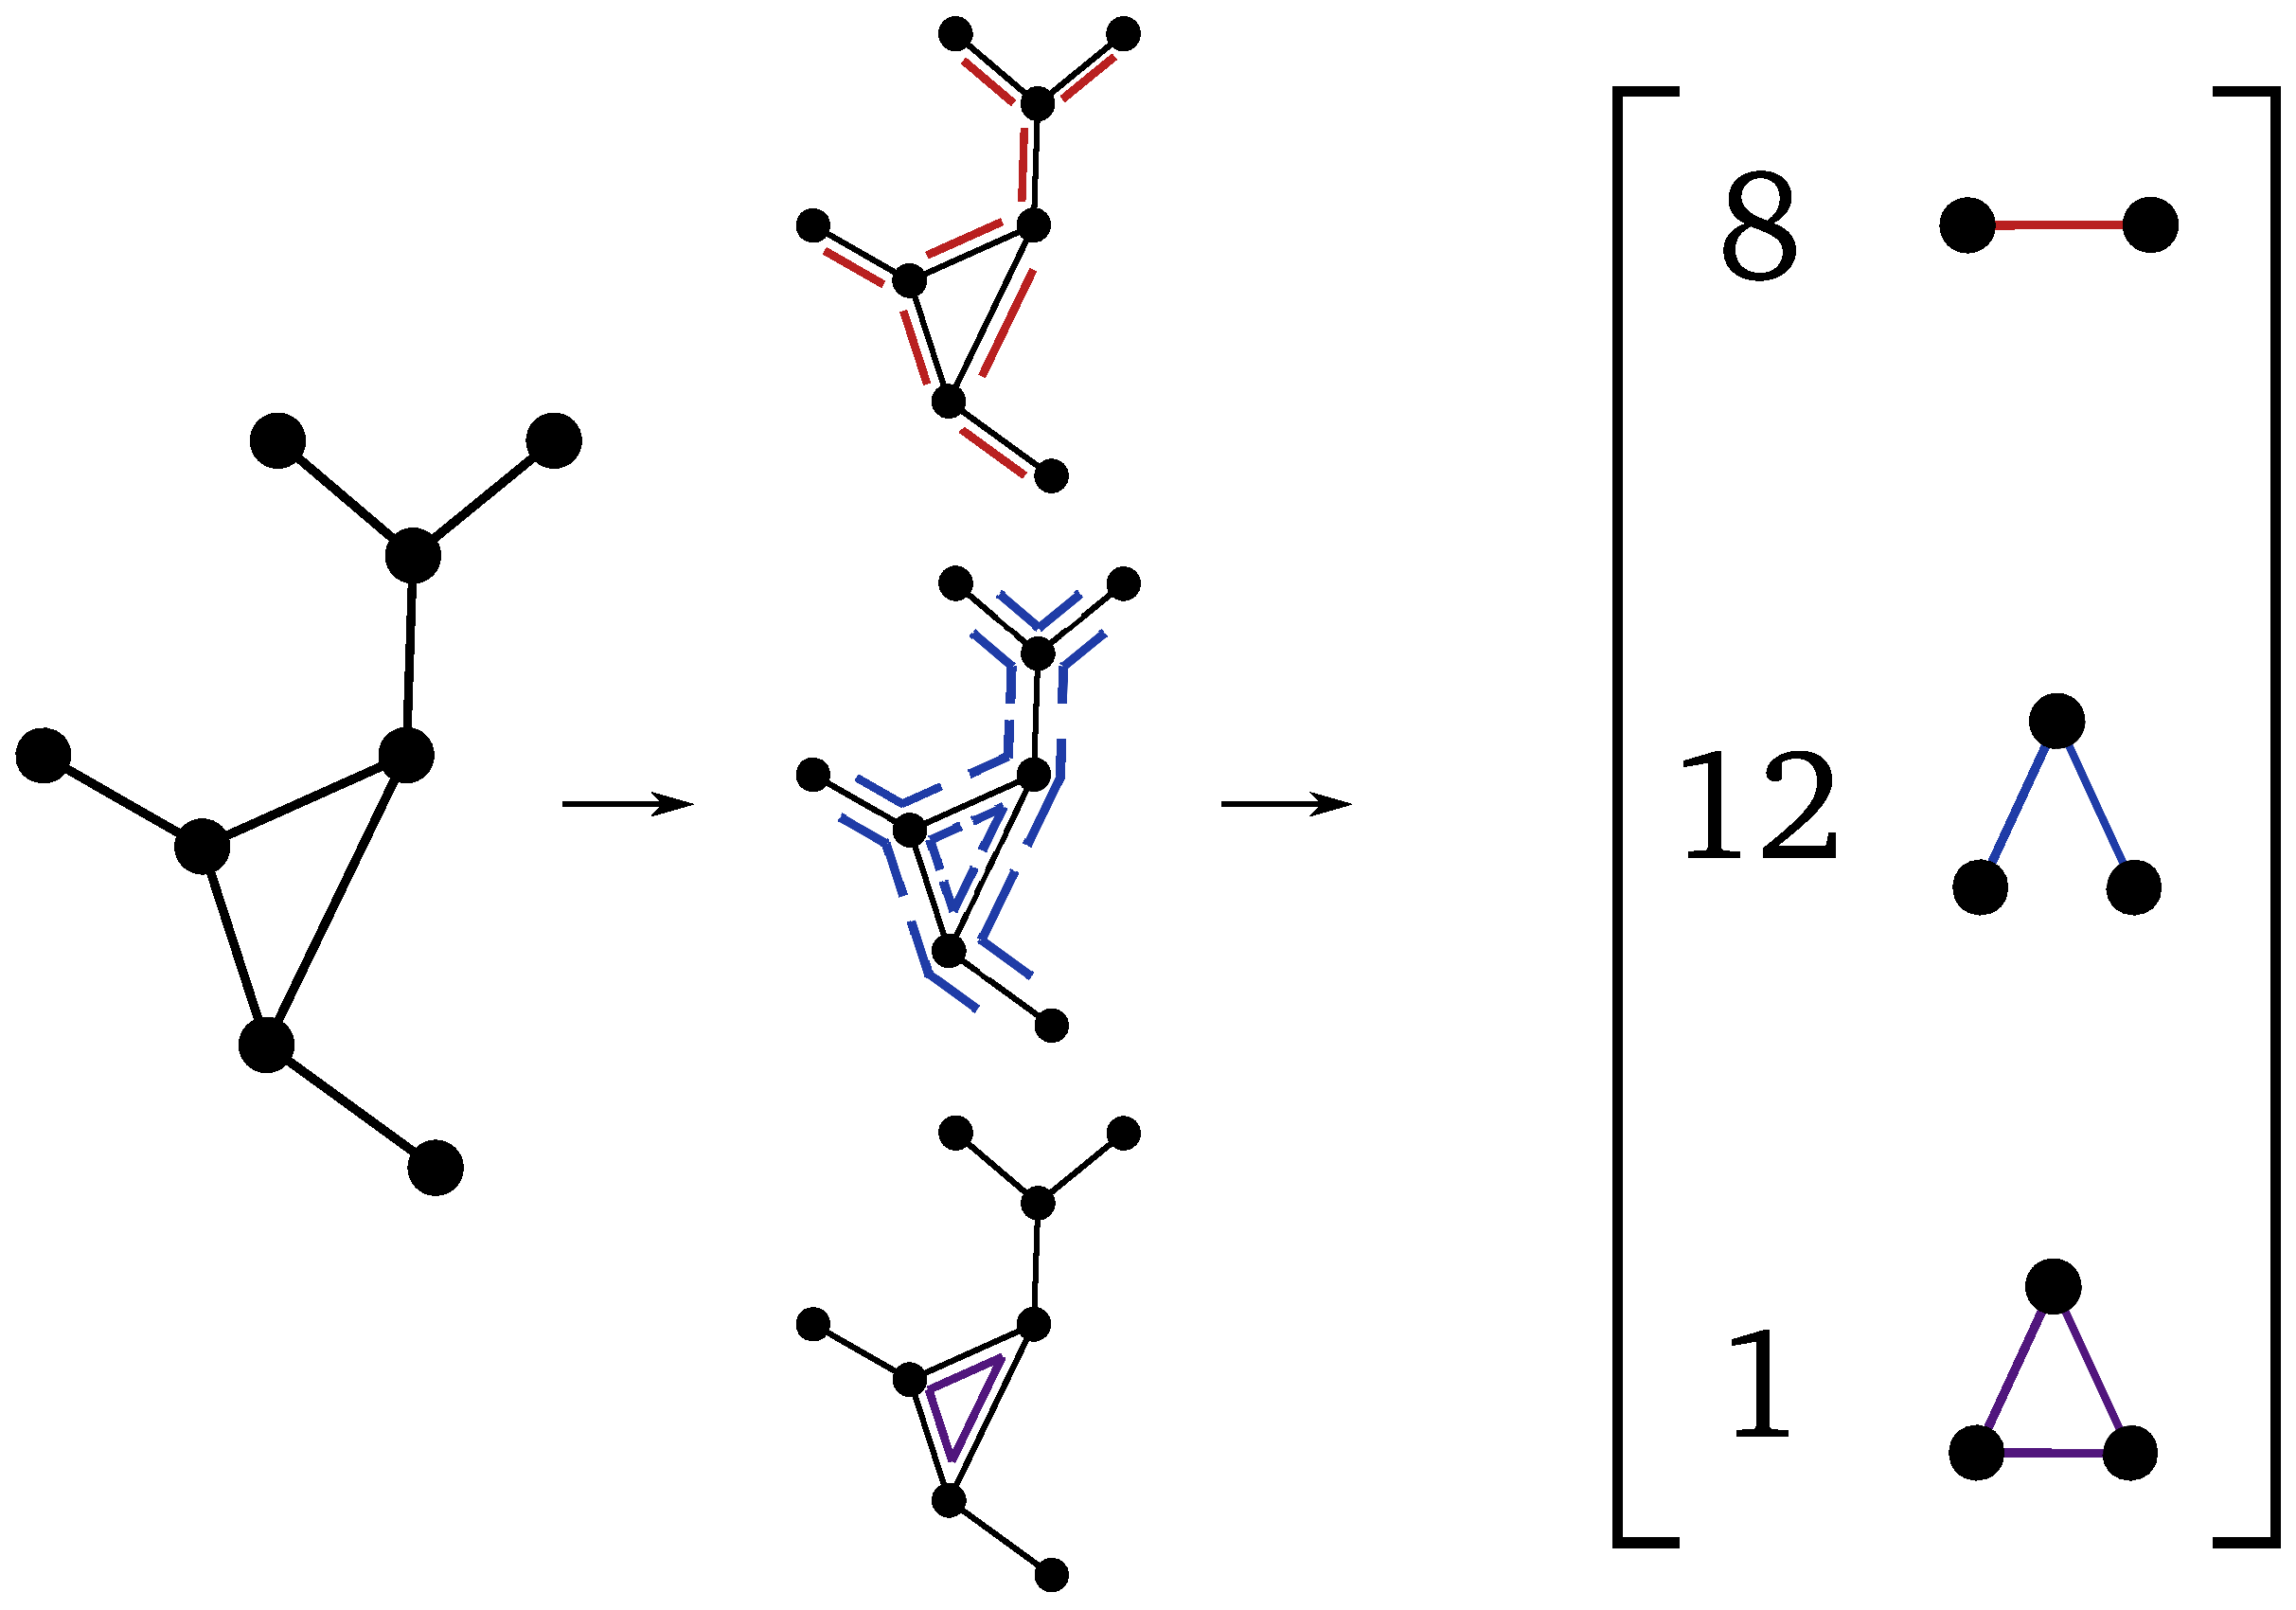
\includegraphics[width=0.9\textwidth]{subgraph-counting}
\caption[Illustration of subgraph-enumeration process for unlabeled graphs]{Illustration of the subgraph-enumeration process with an
  unlabeled input graph. \label{fig:sis4}}
\end{figure}

\begin{figure}[!htp]
\centering
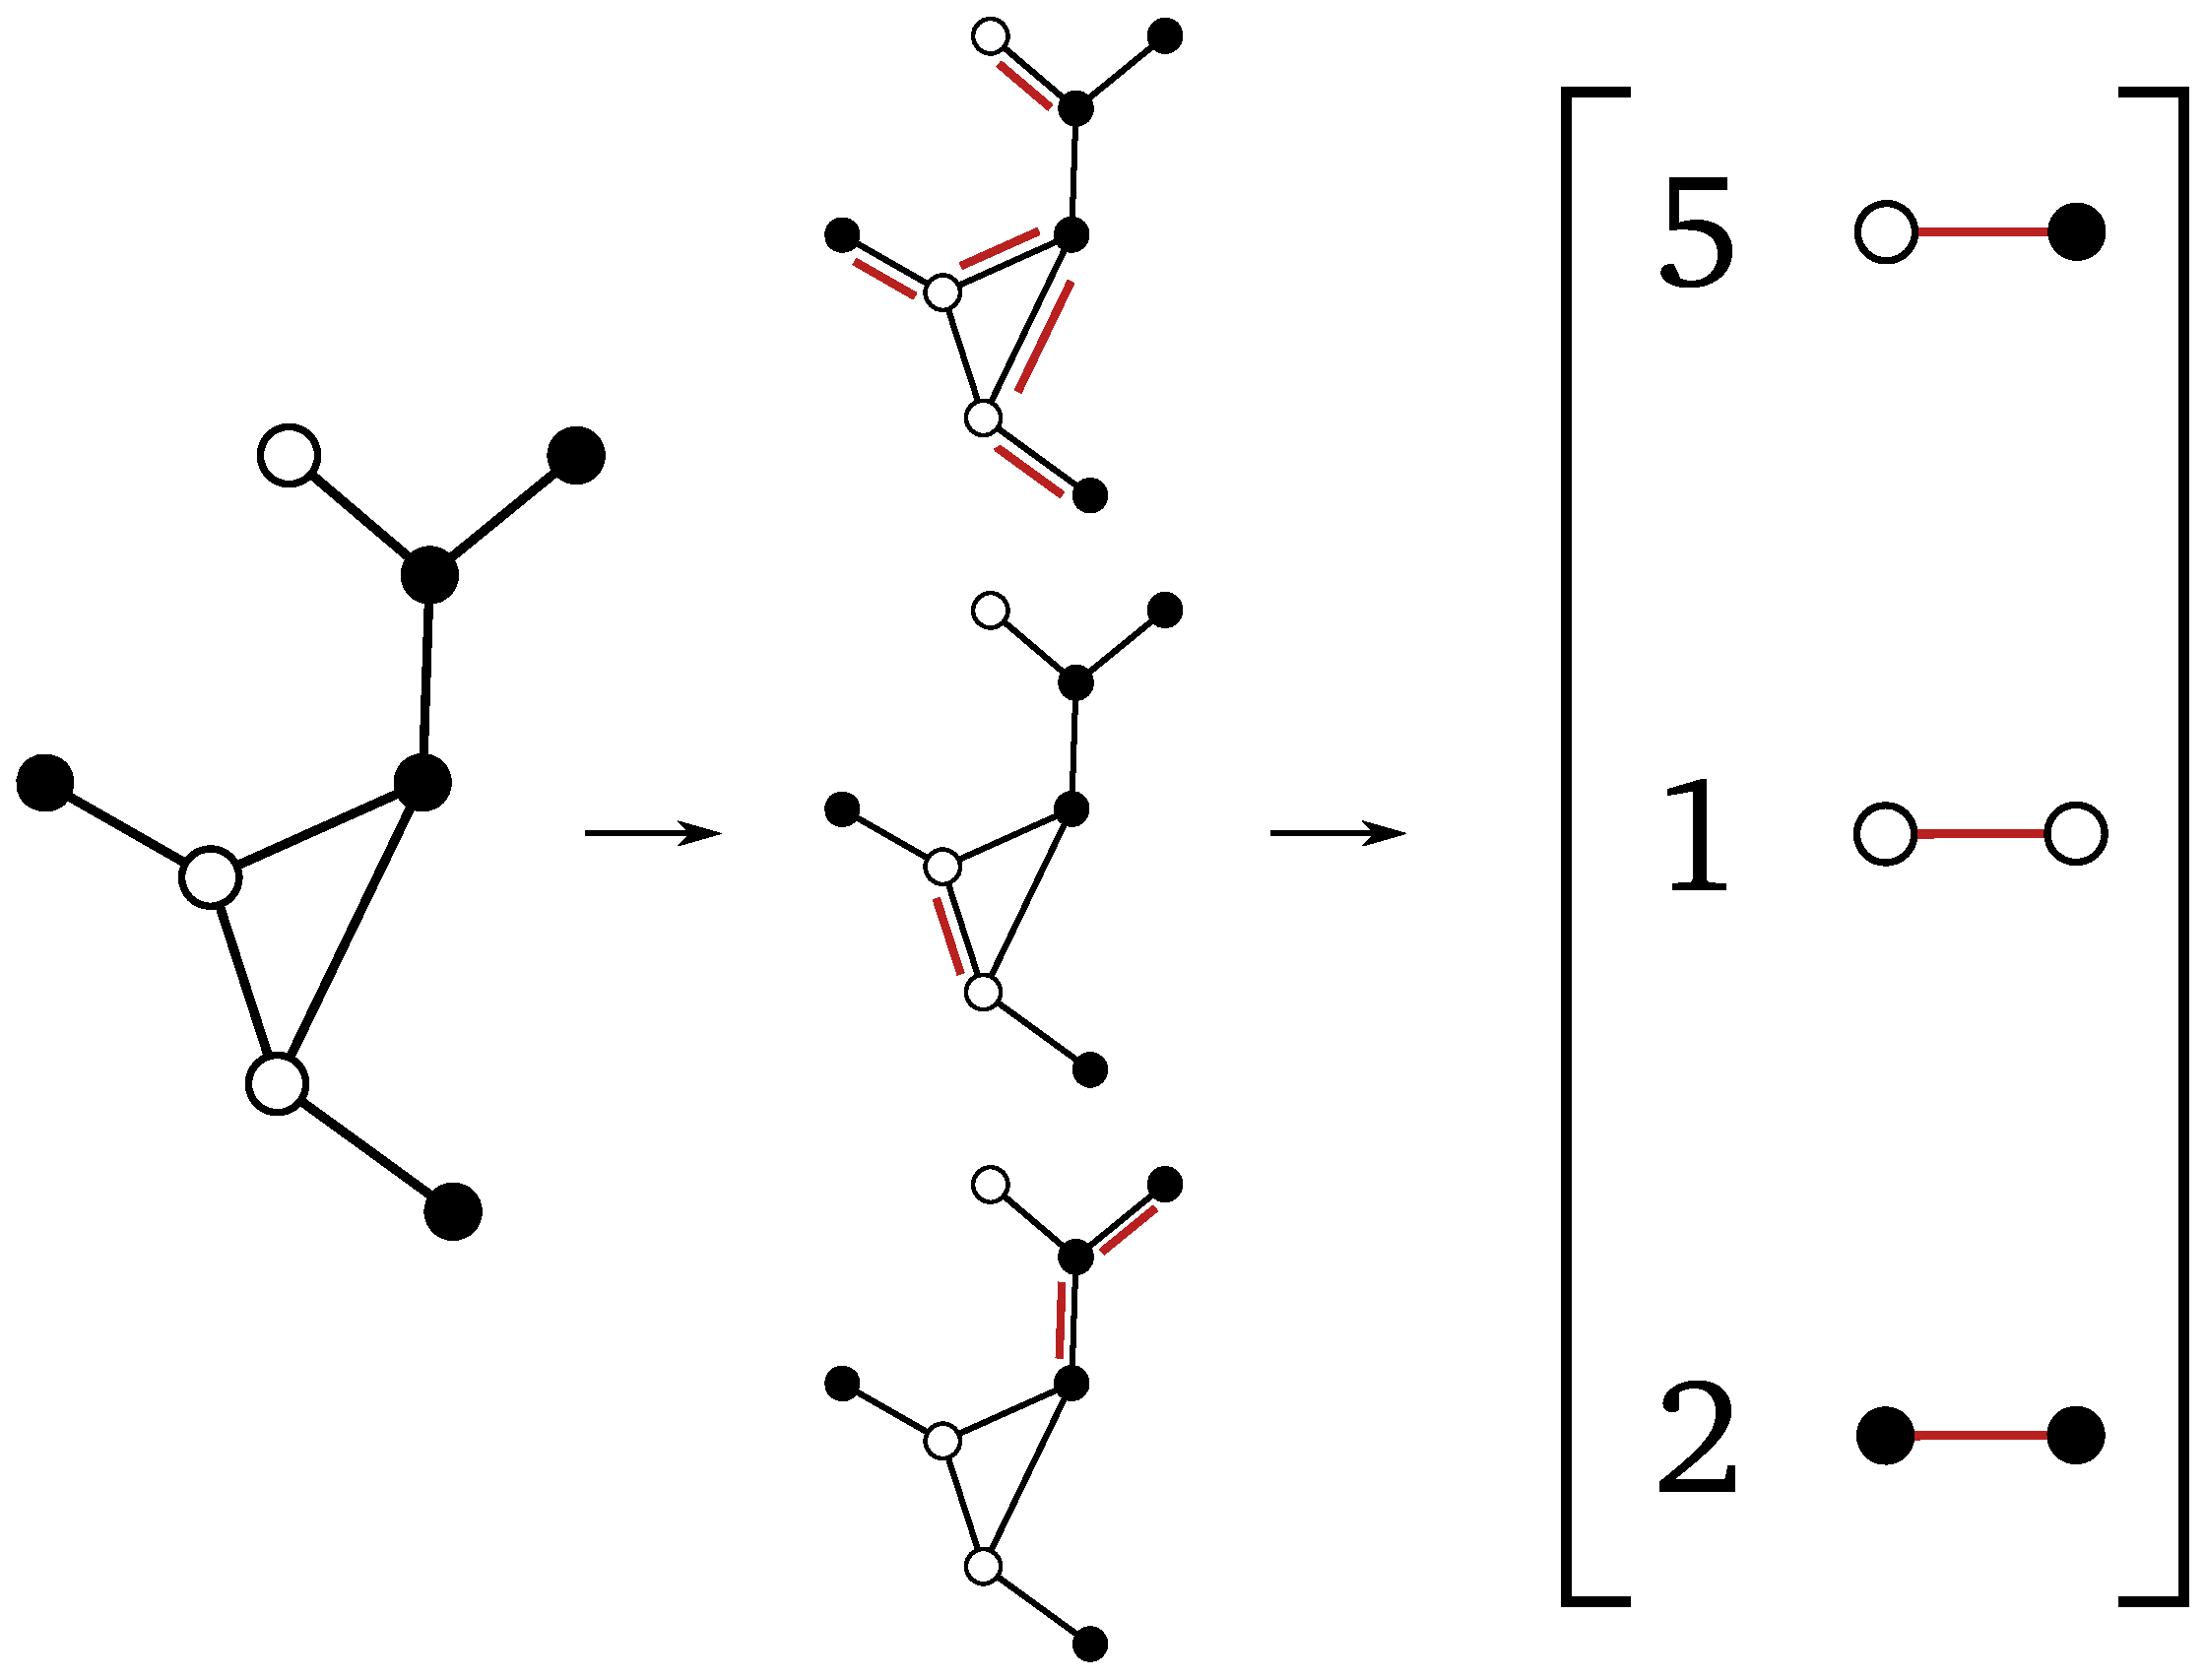
\includegraphics[width=0.9\textwidth]{subgraph-counting-labeled}
\caption[Illustration of subgraph-enumeration process for labeled graphs]{Illustration of the subgraph-enumeration process with a
  labeled input graph. In this case, we must discriminate between
  differently labeled subgraphs. \label{fig:sis5}}
\end{figure}

\section{An unlabeled graph example: the Watts-Strogatz model}

To validate the applicability of the above approach/graph similarity
measure on graph objects, we used the Watts-Strogatz (WS) network
generation model to construct a graph object dataset on which to apply
DMAPS. For a fixed graph size, the WS model relies on two parameters
to generate a so-called small-world network output
\cite{watts_collective_1998}. The first parameter $p$ is initially
used to generate a two-dimensional lattice where each vertex is
connected to all of its neighbors situated a distance at most $p$
away. For each vertex in the graph, we choose the edge that connects
it to its nearest neighbor and, with probability $r$, rewire this edge
to connect with a vertex chosen uniformly at random from the
graph. This procedure is repeated, each time considering the edge that
connects the next closest neighbor to the vertex in question until all
edges have been considered once, with no duplicate edges allowed. The
resulting graph is considered the output of the model. The networks
produced by this model exhibit various qualitatively different
properties as its “generating parameters” vary. For $r=1$ the model
reduces to generating an Erdős–Rényi random graph $G(n,p)$: a graph of
size $n$ for which the probability that any two vertices are connected
is $p$. On the other hand, for $r=0$ the graph remains a regular
lattice, with no random changes in its topology. Lastly, for
intermediate values of $r$ we get many local connections between
adjacent nodes and few edges between far away nodes, which is a
defining characteristic of small-world networks. These different
regimes are depicted in Figure~\ref{fig:sis6a}.

The WS algorithm was used to generate $n=2000$ different small-world
graphs, each with $n=100$ vertices. For each such graph
$G_i(p_i, r_i)$, we generated uniformly at random the two variables
$r_i ~ \mathrm{unif}[0,1]$ and $p_i ~ \mathrm{unif}[0,1]$. We thus are
confident that, by construction, this is a two-parameter set of graph
data, parameterized by the generating parameters $p$ and $r$. The
diffusion map embedding was then constructed by using the graph
similarity measure defined above. It was found that the first two
principal DMAP eigenvectors $\phi_2$ and $\phi_3$ were sufficient to
represent the data. This is confirmed by the two dimensional nature of
the $(\phi_2, \phi_3)$ manifold, shown in Figure~\ref{fig:sis6bc}
colored by $\log(r)$ and $p$. When considering the values of $p_i$ and
$r_i$ of the various data points (the various graphs) that lie on this
two-dimensional manifold, it can be observed that they vary in
directions visually independent of each other. This strongly suggests
that the transformation $f:(\phi_2, \phi_3) \rightarrow (r,p)$ has a
nonsingular Jacobian matrix, which in turn implies that the
transformation is bijective - the two variable pairs are one-to-one
with each other, and they each constitute coordinates of the network
dataset. This means that DMAPS discovered a reparameterization of the
two variables $r$ and $p$, which in this case were known in advance to
be (by construction) the variables that define this dataset. This
serves as a validation for the DMAPS approach and the chosen graph
similarity measure since, by only examining a dataset generated by the
WS model, the technique was able to “learn” that only two features
mattered, and that the two features were one-to-one with the
construction parameters $(r, p)$ that here were a priori known.


\begin{figure}[!htp]
\centering
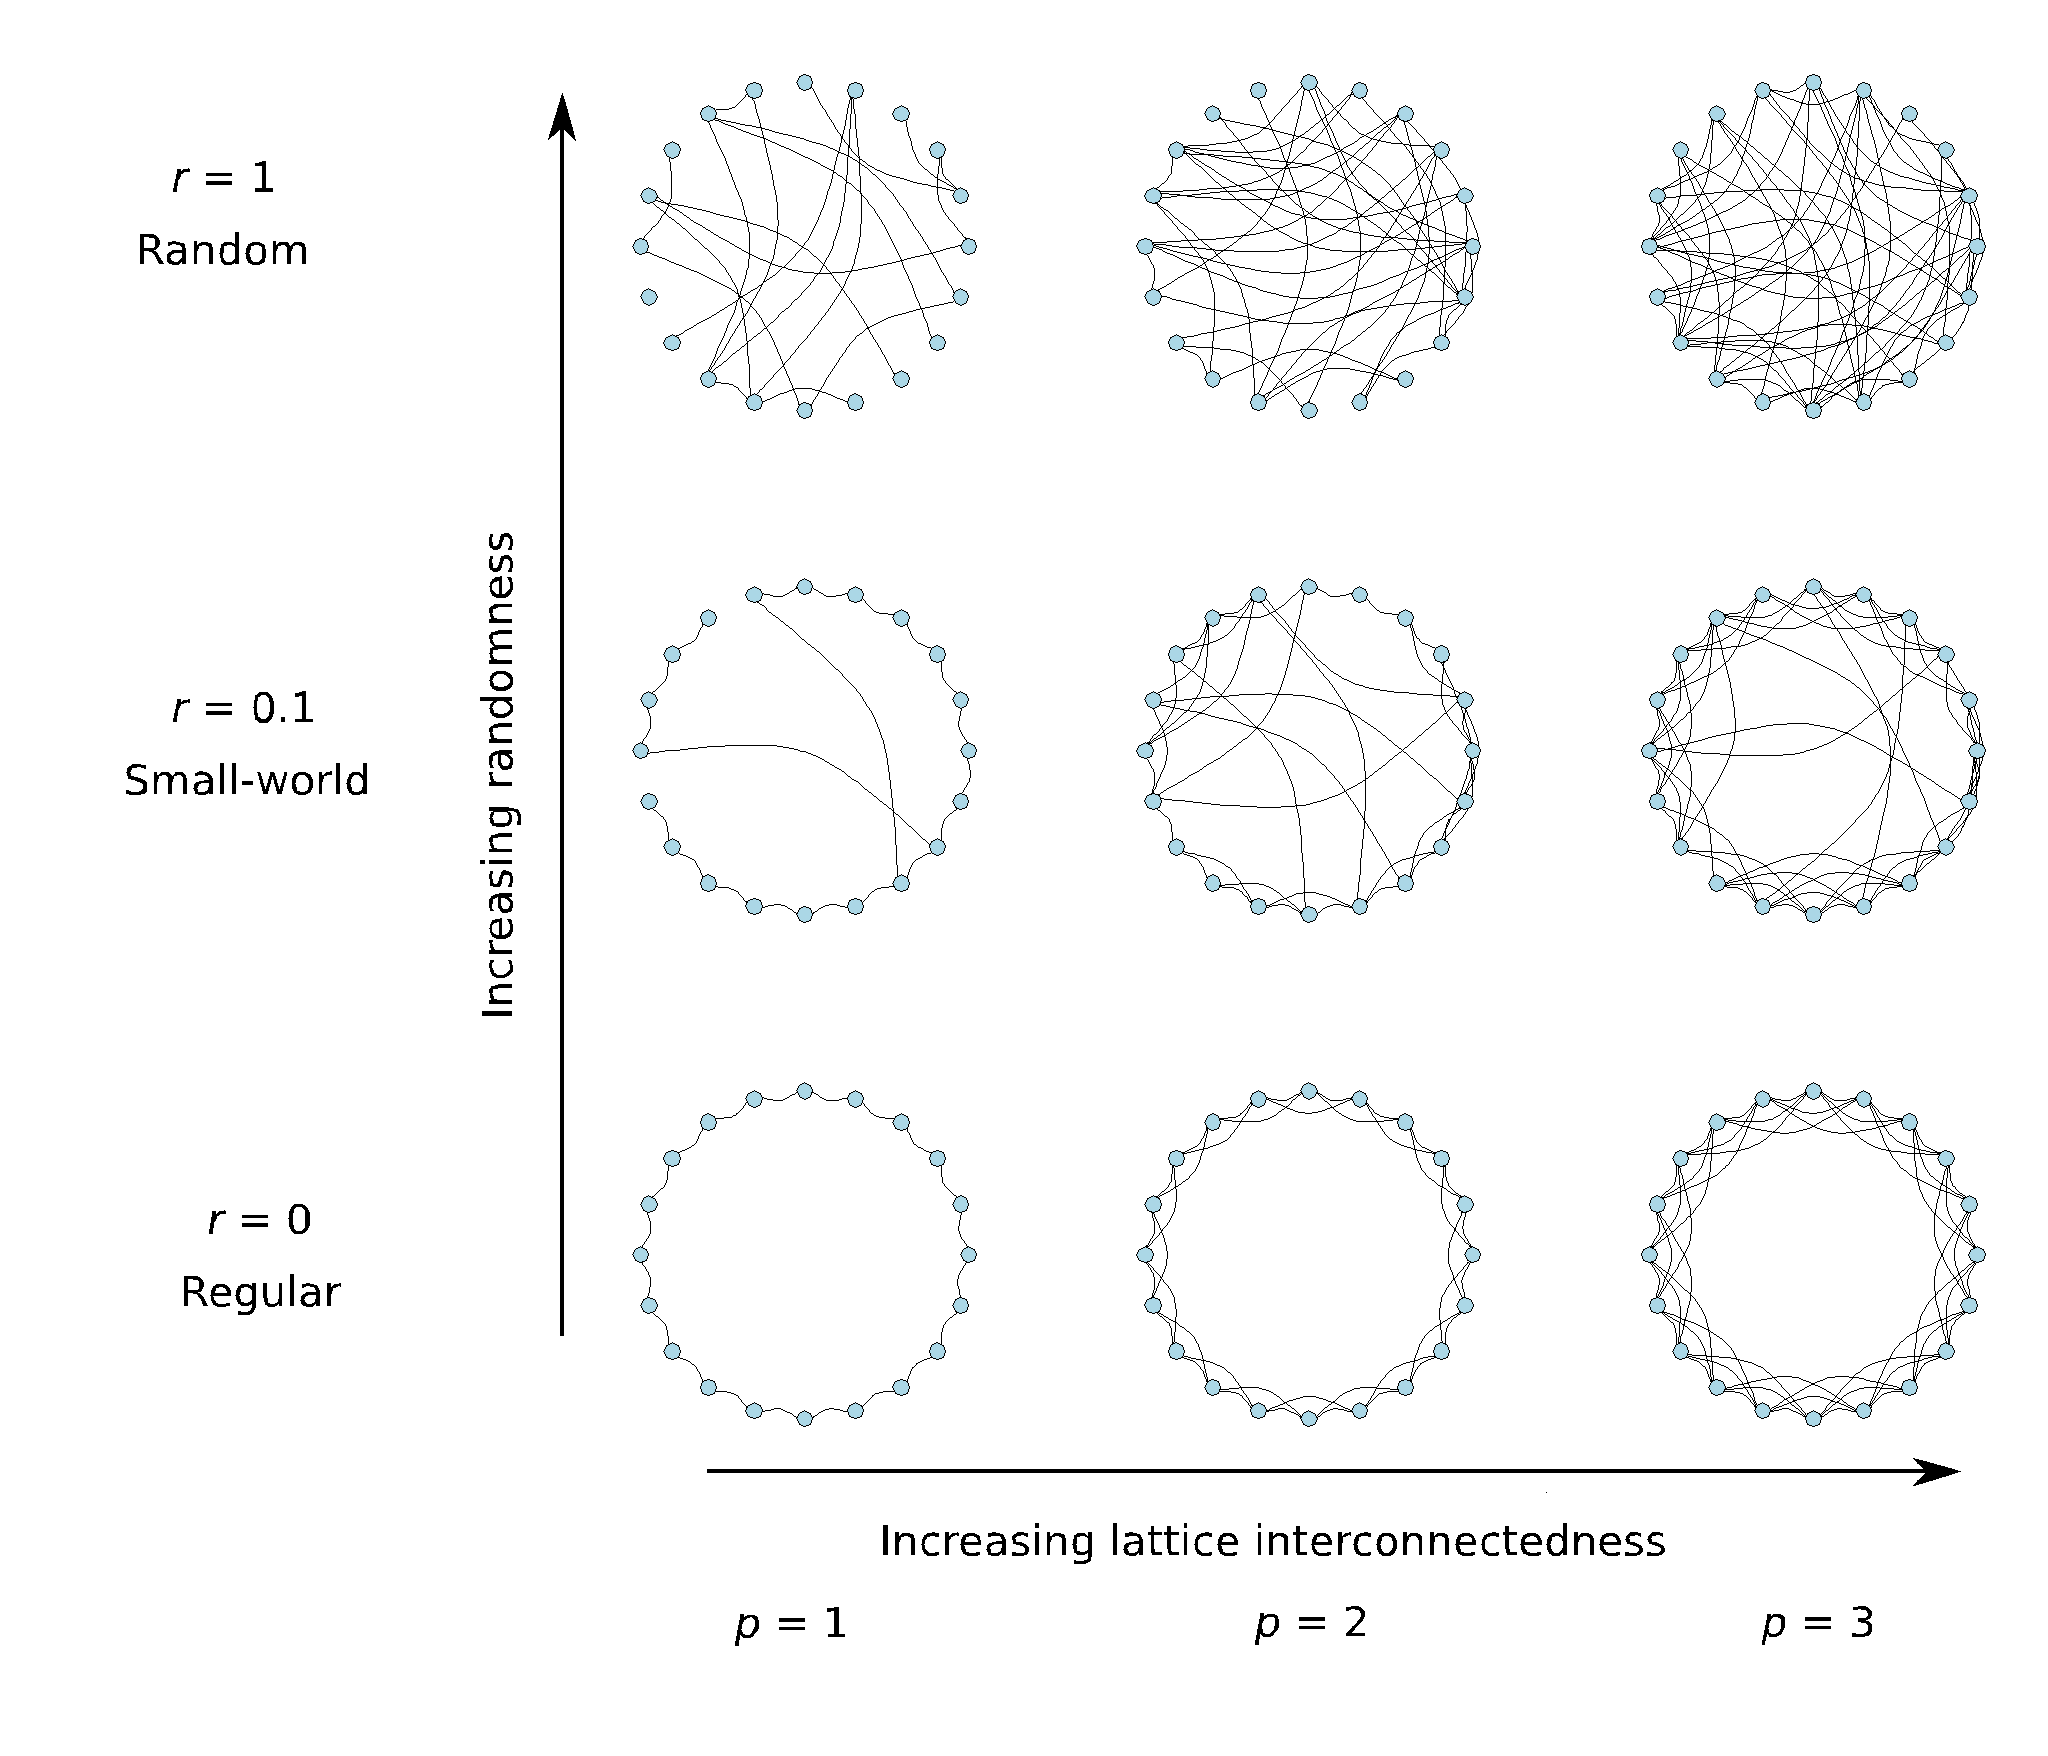
\includegraphics[width=0.9\textwidth]{6a}
\caption[Variations of Watts-Strogatz model]{The Watts-Strogatz model and its construction parameters:
  The value of $r$ denotes the probability of long-distance rewiring
  with $r = 0$ denoting a regular lattice, $r < 1$ a small-world graph,
  and $r = 1$ an Erdős–Rényi random graph. The value of $p$ quantifies how
  interconnected the initial lattice is, being the number of
  neighboring nodes each node connects to. \label{fig:sis6a}}
\end{figure}

\begin{figure}[!htp]
\centering
\begin{tabular}{cc}
  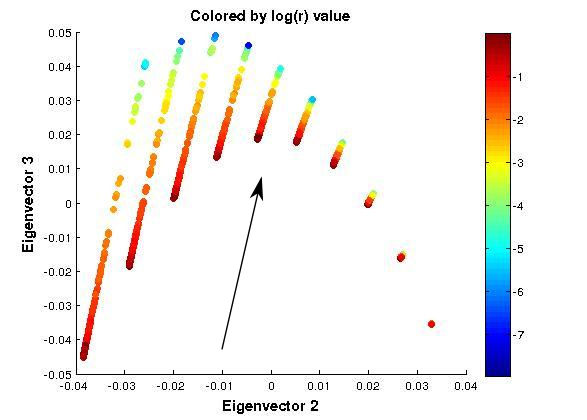
\includegraphics[width=0.45\textwidth]{6b} &
  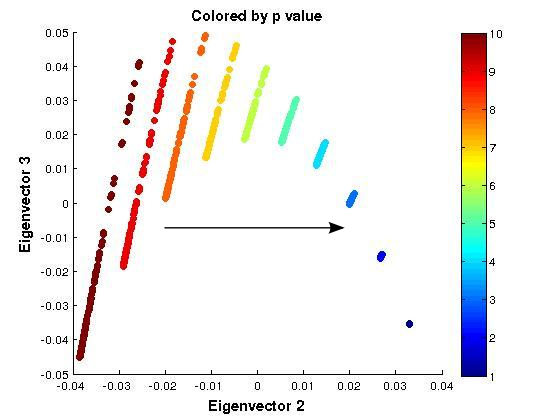
\includegraphics[width=0.45\textwidth]{6c}\\
  (a) & (b)
\end{tabular}
\caption[DMAPS results on Watts-Strogatz networks]{(a) Second versus third eigenvector $(\phi_2 ,\phi_3)$
  colored by $\log(r)$ (a) and $p$ (b). The visual linear independence
  of the directions of change of $\log(r)$ and $p$ indicate that the
  $(\phi_2 ,\phi_3)$ coordinates form a bijection with (a
  reparameterization of) the construction parameters $(r, p)$. An
  $\epsilon$ of 0.1 was used in our DMAPS
  computations. \label{fig:sis6bc}}
\end{figure}


\section{SIS model results}

In order to identify the coarse variables that parameterize the
dynamics of the adaptive SIS model, DMAPS were implemented on a graph
dataset sampled from the SIS model evolution. This dataset was
generated by systematically sampling graph objects from the SIS model
simulation over time from various parameters/initial conditions, with
each simulation leading to different long-term dynamical behavior. The
principal directions, represented by the leading diffusion map
coordinates, identify the important variables that define the model's
evolution over time. Since the set of coarse variables
$(i, l_{II}, l_{SS})$ are known to be central to the model's
evolution, their relationship with the derived principal directions
was investigated \cite{gross_robust_2008}.

More specifically, the system is known to undergo a Hopf bifurcation
to periodic solutions as the parameter $p$ varies around
$(p, r, w_0) \approx (0.00071, 0.0002, 0.06)$ and graph objects at
parameter values around this bifurcation point were sampled to create
a dataset of $N = 6000$ graphs ${G_i}_{i=1}^N$. After the graphs were
sampled, the DMAPS procedure detailed above was applied, with our
labeled graph metric used as a similarity measure. An analysis of the
relationship between the diffusion map coordinates indicates a
two-dimensional embedding in the first two principal directions
$\phi_2$, $\phi_3$, see Figures~\ref{fig:sis7} (a). Furthermore, an
investigation of the relationship between $\phi_2$ and $\phi_3$ with
other diffusion map coordinates demonstrates that no new direction is
captured by higher order eigenvectors, something that strongly implies
that the manifold on which the dataset lies is indeed
two-dimensional. This is achieved by performing linear regression,
with a suitable kernel, on the eigenvectors and checking whether each
can be accurately reconstructed using the rest, quantified as
cross-validation error, shown in Figures~\ref{fig:sis7} (b). This
measure is high for eigenvectors characterized by unique directions,
and low for higher harmonics and noise. It has the added benefit that
it can be used to compare many eigenvectors, not limiting it only to
the first few.

Motivated by the evidence that the $(\phi_2 ,\phi_3)$ manifold fully
captures all independent directions in the dataset, we look at the
relationship between these two principal directions and the coarse
variables $(i, l_{II}, l_{SS})$ , known to encapsulate the long-term
dynamics of this system. The relationship between $(\phi_2 ,\phi_3)$
and $(i, l_{II}, l_{SS})$ can be investigated by visually studying the
embedding of the coarse variables in diffusion map space. Looking at
the relationship between these three variables in our dataset, it can
be noticed that they actually span two (and not three different)
dimensions, which can be garnered by their two dimensional embedding
in $\mathbb{R}^3$. Thus, we are actually looking for two principal
directions, motivating the definition of
$l_{SI} = L − (l_{II} + l_{SS})$, the total number of SI-links as a
compound variable. This is done without introducing or removing any
information from the system, as the total number of edges is
11constant throughout. We consider $\log(l_{SI})$ as a candidate
macro-variable, since we are interested in finding a bijective
relationship between $(\phi_2 ,\phi_3)$ and $(i, l_{II}, l_{SS})$.

By inspecting the relative directions of $i$ and $\log(l_{SI})$ in the
two dimensional embedding of $(\phi_2 ,\phi_3)$, as shown in
Figure~\ref{fig:sis7} (c) and (d), it becomes apparent that they are
transverse to each other, with the former varying roughly from left to
right and the latter from top to bottom. Such an observation is strong
evidence that the Jacobian of the transformation
$f:(\phi_2, \phi_3) \rightarrow (i, l_{SI})$ is nonsingular on this
dataset, much in the same manner as for the Watts-Strogatz graph
ensembles. Thus, we can conclude that the directions of change on the
$(\phi_2 ,\phi_3)$ manifold represented by changing $i$ and $l_{SI}$,
respectively, are independent of each other, and that they are
reparameterizations of the principal eigenvectors. Similar results are
obtained if we consider $l_{SI}$ instead of $\log(l_{SI})$. These
observations imply that the diffusion map technique has been
successful in identifying, up to parameterization, the variables found
in ~\cite{gross_robust_2008} as responsible for the long term dynamics
of the model. Furthermore, we were able to confirm that the long-term
dynamics of this model really depend on only two macro-variables, the
total number of infected nodes $i$ and the total number of SI-links
$l_{SI}$. Figures~\ref{fig:sis7} (e) and (f) show other colorings of
the $(\phi_2 ,\phi_3)$ plane, and Figure~\ref{fig:sis8} shows the
two-dimensional nature of the system as seen in three dimensions.

In addition, there was no need to take any a priori knowledge about
the model's specifics into account when isolating the important
variables. Instead, we required the development of a suitable
similarity measure between labeled graphs, which can be generalized
for use with other problems (models, datasets) that exhibit completely
different dynamic behavior. This generalization of feature extraction
for high-dimensional systems can assist in developing a framework for
isolating the coarse variables that define graph-based datasets
without resorting to approaches that rely on intuition about the
specific model.


\begin{figure}[!htp]
\centering
\begin{tabular}{cc}
  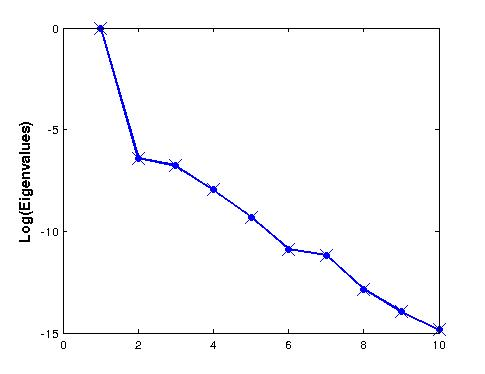
\includegraphics[width=0.45\textwidth]{7a} &
  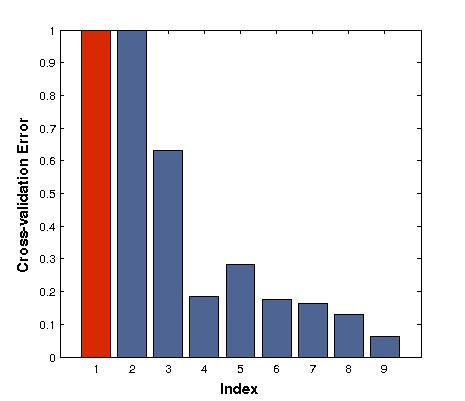
\includegraphics[width=0.45\textwidth]{7b}\\
  (a) & (b)\\
  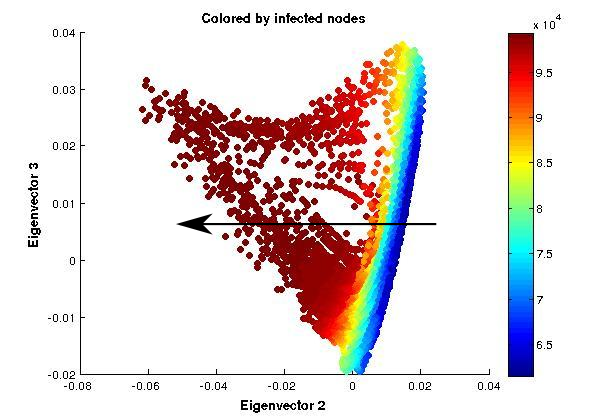
\includegraphics[width=0.45\textwidth]{7c} &
  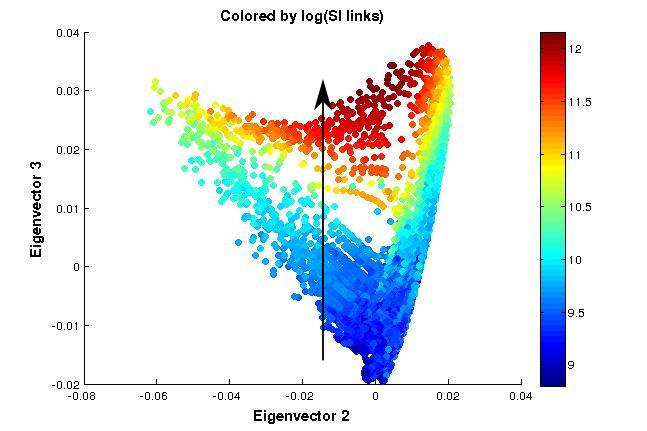
\includegraphics[width=0.45\textwidth]{7d}\\
  (c) & (d)\\
  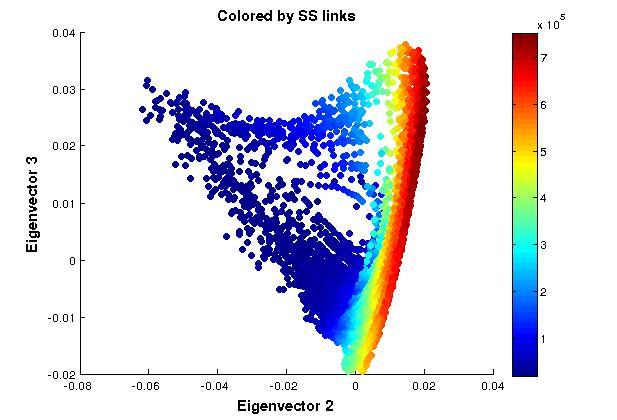
\includegraphics[width=0.45\textwidth]{7e} &
  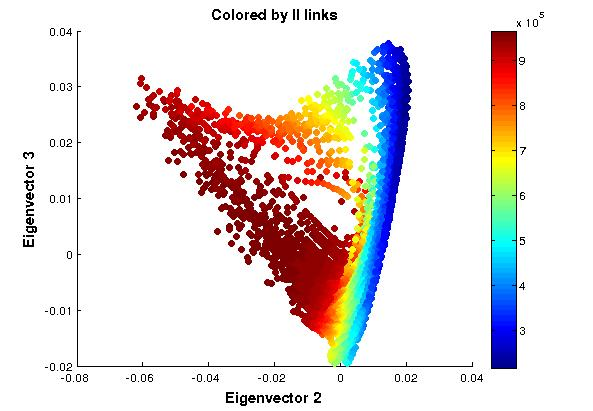
\includegraphics[width=0.45\textwidth]{7f}\\
  (e) & (f)
\end{tabular}
\caption[DMAPS results on SIS networks]{Coarse variable detection: (a) The leading eigenvalues of the
  random walk matrix are plotted. (b) Computational criterion
  suggesting that the first two eigendirections suffice (the first is
  a trivial one, and the third is much less important than the first
  two. The $x$ and $y$ coordinates of the middle and bottom row
  figures indicate the components of each datum, representing a graph,
  in the second and third eigenvectors of the random walk matrix. Each
  point is also colored by the number of (c) infected nodes $i$, (d)
  $\log$(SI-links), (e) SS-links, and (f) II-links found in the
  corresponding graph. A comparison between (c) and (d) indicates a
  linear independence relationship between $i$ and $log(l_{SI})$. An
  $\epsilon$ of 70 was used. \label{fig:sis7}}
\end{figure}

\begin{figure}[!htp]
\centering
\begin{tabular}{cc}
  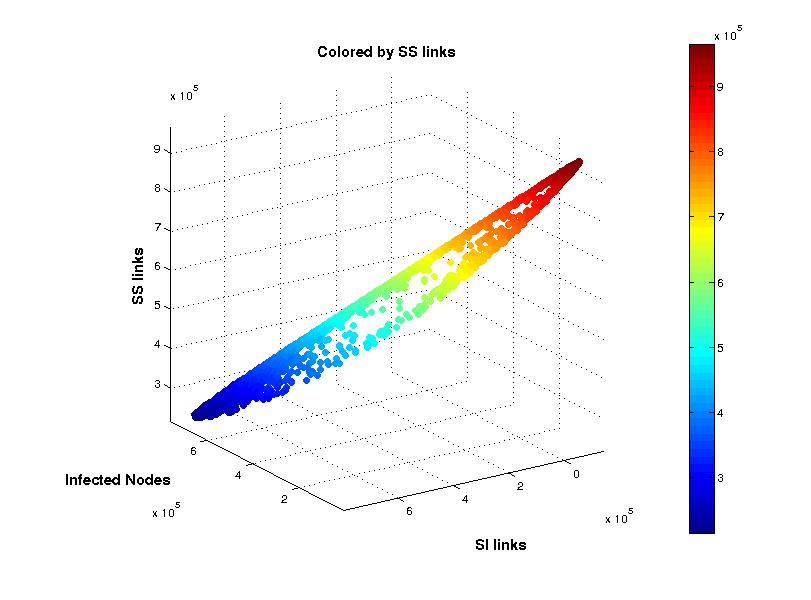
\includegraphics[width=0.45\textwidth]{8a} &
  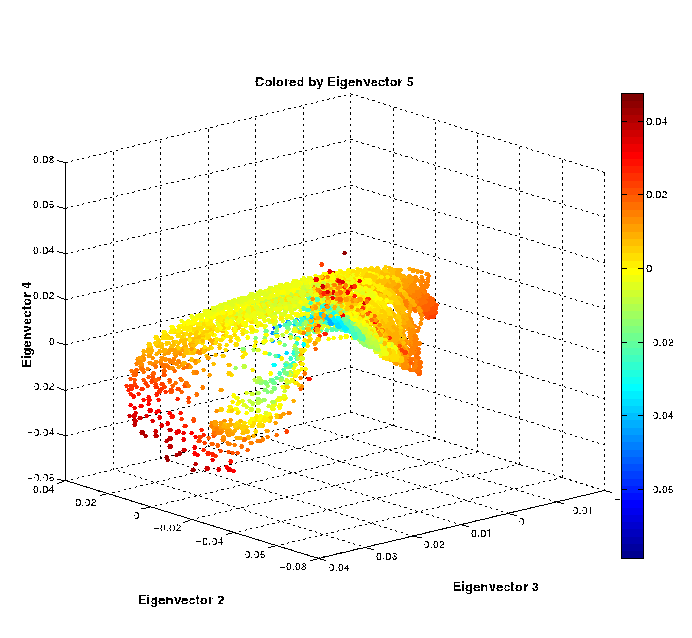
\includegraphics[width=0.45\textwidth]{8b}\\
  (a) & (b)
\end{tabular}
\caption[Another view of DMAPS results on SIS networks]{Coarse Variable Dependencies: An illustration of the
  relationship between $l_{SS}$, $l_{SI}$, and $i$ in the diffusion
  map dataset. The two-dimensional nature of the manifold indicates
  that the number of SS links can be thought of as a function, on the
  data, of $i$ and $l_{SI}$, and is thus not necessary as an
  independent macro-variable. \label{fig:sis8}}
\end{figure}


\section{Conclusion}

The use of networks in the modeling of real-world phenomena is
particularly suited to modeling the spread of an epidemic through a
population represented as a network of geographic/social
connections. In this paper, the suitability of data mining techniques
for extracting the important macro-variables describing the evolution
of network connectivity from an adaptive SIS model were investigated,
based on two concepts. Firstly, a dissimilarity metric for graph
objects was constructed; secondly, it was used with the DMAPS
nonlinear data-mining procedure. In particular, we needed to define a
(dis)similarity measure between different labeled graphs, as they
arise in the course of the epidemic model simulation. It should be
noted that this method is generalizable to any labeled graph with
distinct labels, and can be utilized regardless of the overarching
process defining graph evolution. Future work in this area should
investigate the suitability of other graph similarity measures for use
within the DMAPS framework. Moreover, this approach is not DMAPS-
specific. Indeed, other non-linear data mining techniques are expected
to yield similar results, provided they use the aforementioned
dissimilarity measure.

In addition, the long-term dynamics of a particular adaptive SIS model
were explored, which allowed us to verify the suitability of the
constructed metric for use with graph object datasets. This yields two
interconnected results. Firstly, the DMAP procedure was able to
demonstrate that the system is inherently macroscopically two
dimensional, with the two independent directions in the dataset being
represented by the first two nontrivial Diffusion Map
eigenvectors. This result is consistent with previous knowledge about
the dimensionality of the model’s dynamics, and is strong evidence
that the DMAP framework, using the similarity measure we constructed,
can be readily applied to graph object data sets to extract meaningful
reduced parameterizations of the underlying behavior.

Furthermore, we were also able to link the principal diffusion map
coordinates with previously known coarse variables capable of
describing this system. By inspection of the embeddings in diffusion
space, it was verified that a bijection exists between two of these
coarse variables and the two leading diffusion map coordinates. This
means that the DMAP was not only able to learn the inherent
dimensionality of the dataset, but that it was also able to extract a
reparameterization of variables known to fully specify this model;
what is unfortunate, is that the variables of this reparameterization
have no obvious unique, easily explainable physical meaning.

This modeling exercise clearly shows that modern data mining
techniques for data in the form of high-dimensional evolving vectors
can be extended to data in the form of large evolving graphs (labeled
or unlabeled). This holds promise for the analysis of data from
epidemics on realistic adaptive networks, and for general adaptive
network evolution problems. What is more important and more promising,
however, is that these data-based coarse descriptors can be used, in
an equation-free framework, to implement accurate reduced model
computations for the epidemic dynamics, in which the variables used to
describe the systems-level network behavior are the ones obtained from
data mining. This data-driven model reduction approach can be
introduced as a “wrapper algorithm” around brief bursts of detailed,
fine scale simulation; we believe that the approach holds real promise
in enabling systems level analysis, simulation and control of
detailed, realistic epidemic dynamics.

We have now seen two unique applications of DMAPS to network
systems. The next chapter will again employ this nonlinear manifold
learning technique, but in a different application. We will see how
DMAPS can be used to uncover important parameter combinations in
systems of differential equations.



%%% Local Variables: ***
%%% mode:latex ***
%%% TeX-master: "../../thesis.tex"  ***
%%% End: ***
\chapter{Identifying significant parameters combinations in complex
  models \label{ch:params}}


% \begin{abstract}
%   Detailed dynamical models can often be summarized in terms of only
%   a few components, reducing complexity and making exploration
%   easier and more insightful.  Pen-and-paper reduction is tedious
%   and impractical for most models, however it has the added benefit
%   of identifying parameter combinations that matter most.  Recently
%   developed frameworks computerizing model reduction leave the dual
%   aspect of effective parameter identification unaddressed,
%   relegating parameter space exploration subject to ineffective
%   sampling strategies.  Here, we lay the foundation for systematic
%   parameter reduction, rooting it in the same nonlinear data mining
%   techniques that powered model reduction in our earlier
%   equation-free framework.  Our ambition is to extend the
%   data-driven determination of effective variables by integrating
%   into it the discovery of effective model parameters.  This will
%   accelerate both dynamical simulations and parametric explorations,
%   allowing us to efficiently map out the behavior of complex models.

% \end{abstract}

The past decades have seen a steady fall in the cost of computation,
enabling systems to be studied using increasingly complex models.
Perceptron networks in the 1960's contained thousands of hidden units
\cite{nagy_neural_1991}, while modern neural nets are comprised of
billions \cite{hsu_biggest_2015}. Molecular dynamics simulations in
1957 entailed tens of hard-sphere particles \cite{alder_phase_1957};
today we model entire proteins and their folding dynamics
\cite{piana_atomic-level_2013}. And Lorenz's three-dimensional system
of equations describing atmospheric convection in 1963
\cite{lorenz_deterministic_1963} led to modern large eddy simulations
run across multiple computing clusters \cite{ghosal_dynamic_1995}. In
all cases, the improvement in precision afforded by increased model
complexity is matched by an increased number of model parameters.

Highly parameterized models may aid accuracy, but the effect of each
individual parameter on the overall model output is often difficult to
ascertain. Indeed, it has been well-document that a wide array of
systems contain particular hidden parameters that appear to have no
influence on the model's predictions
\cite{gutenkunst_extracting_2007}. These have been termed ``sloppy
parameters'', and their presence seems ubiquitous in contemporary
systems \cite{gutenkunst_universally_2007}. This is problematic as not
only do sloppy parameters obfuscate the inputs that actually
matter, but they also lead to slow convergence of model-fitting
algorithms \cite{transtrum_geometry_2011}.

Several approaches have been suggested to combat this
over-parameterization. Some, such as the Manifold Boundary
Approximation Method ultimately rely on deriving by hand a reduced
model \cite{transtrum_model_2014}. Others, such as Active Subspaces
make assumptions about linearity that may not hold in practical
settings \cite{constantine_active_2015}. Here, we present a
data-driven approach to parameter reduction that is flexible enough to
handle nonlinear systems. This is accomplished through Diffusion Maps
(DMAPS), an established manifold learning technique that we adapt to
this context \cite{coifman_diffusion_2006}. We begin with a
description of our formulation of the problem, and then present a
simple example that clearly shows the consequences of sloppiness,
while also providing some intuition as to how it emerges.

Our overall approach is motivated by the work in
\cite{transtrum_geometry_2011}. We consider a model to consist of a
vector of parameters $\theta \in \mathbb{R}^k$ and a function mapping
these inputs to a model response (or model output) in $\mathbb{R}^n$,
$f: \mathbb{R}^k \rightarrow \mathbb{R}^n$. Sloppiness would reveal
itself as regions of parameter space, $\Omega_S \in \mathbb{R}^k$ in
which the model reponse remains nearly constant:
$f(\theta_i) \approx f(\theta_j)\; \theta_i, \theta_j \in
\Omega_S$. We will also denote distances in parameter space as
$\delta(\theta_i, \theta_j) = \| f(\theta_i) - f(\theta_j)\|_2$, that
is, the Euclidean distance between the resulting model responses. To
provide a concrete example, consider a model with parameters $p_1$ and
$p_2$, and model output
$f(p_1, p_2) = (p_1 p_2 , \ln(p_1) + \ln(p_2) , (p_1 p_2)^2)$. Then
$\theta = (p_1, p_2) \in \mathbb{R}^2$ and $f: \R^2 \rightarrow
\R^3$. It is clear from the expression for $f$ that the model response
depends only on the overall product $p_1 p_2$, and not on $p_1$ and
$p_2$ independently. To make it explicit, set $p_{eff} = p_1 p_2$ and
rewrite $f$ as $(p_{eff}, \ln(p_{eff}), p_{eff}^2)$. Thus, although we
have chosen to include both $p_1$ and $p_2$ as independent parameters
in our original model, only the value of $p_{eff}$ is significant. Also note
that if we only had access to a black-box function evaluator, it would
be non-trivial to determine the existence of $p_{eff}$ at all.

This model is illustrated in Figure~\ref{fig:non-id}, where curves of
constant color denote sets of constant model response. If we had
sampled data corresponding to true parameter values of
$p_1^* = p_2^* = 1$, Figure~\ref{fig:non-id} also reveals how
sloppiness affects optimization routines trying to fit such
data. Convergence is permitted along entire bands of parameter space
instead of at a single point. The inset shows $\delta$-contours of a
slightly perturbed system in which both $p_1$ and $p_2$ influence $f$;
however, certain directions, namely along the diagonal, still affect
model output more strongly than others. In addition, optimization
routines will still converge to disparate points in the plane: the
model remains sloppy.

Our goal, then, is to extract the appropriate, intrinsic
parameterization of the model using only input-output data. As we
shall see, this parameterization may vary across input space regimes.
We will show how this variation can be associated with the traditional
notions of regular and singular perturbations in explicit models when
the number of effective parameters changes.


\begin{figure}
  \centerline{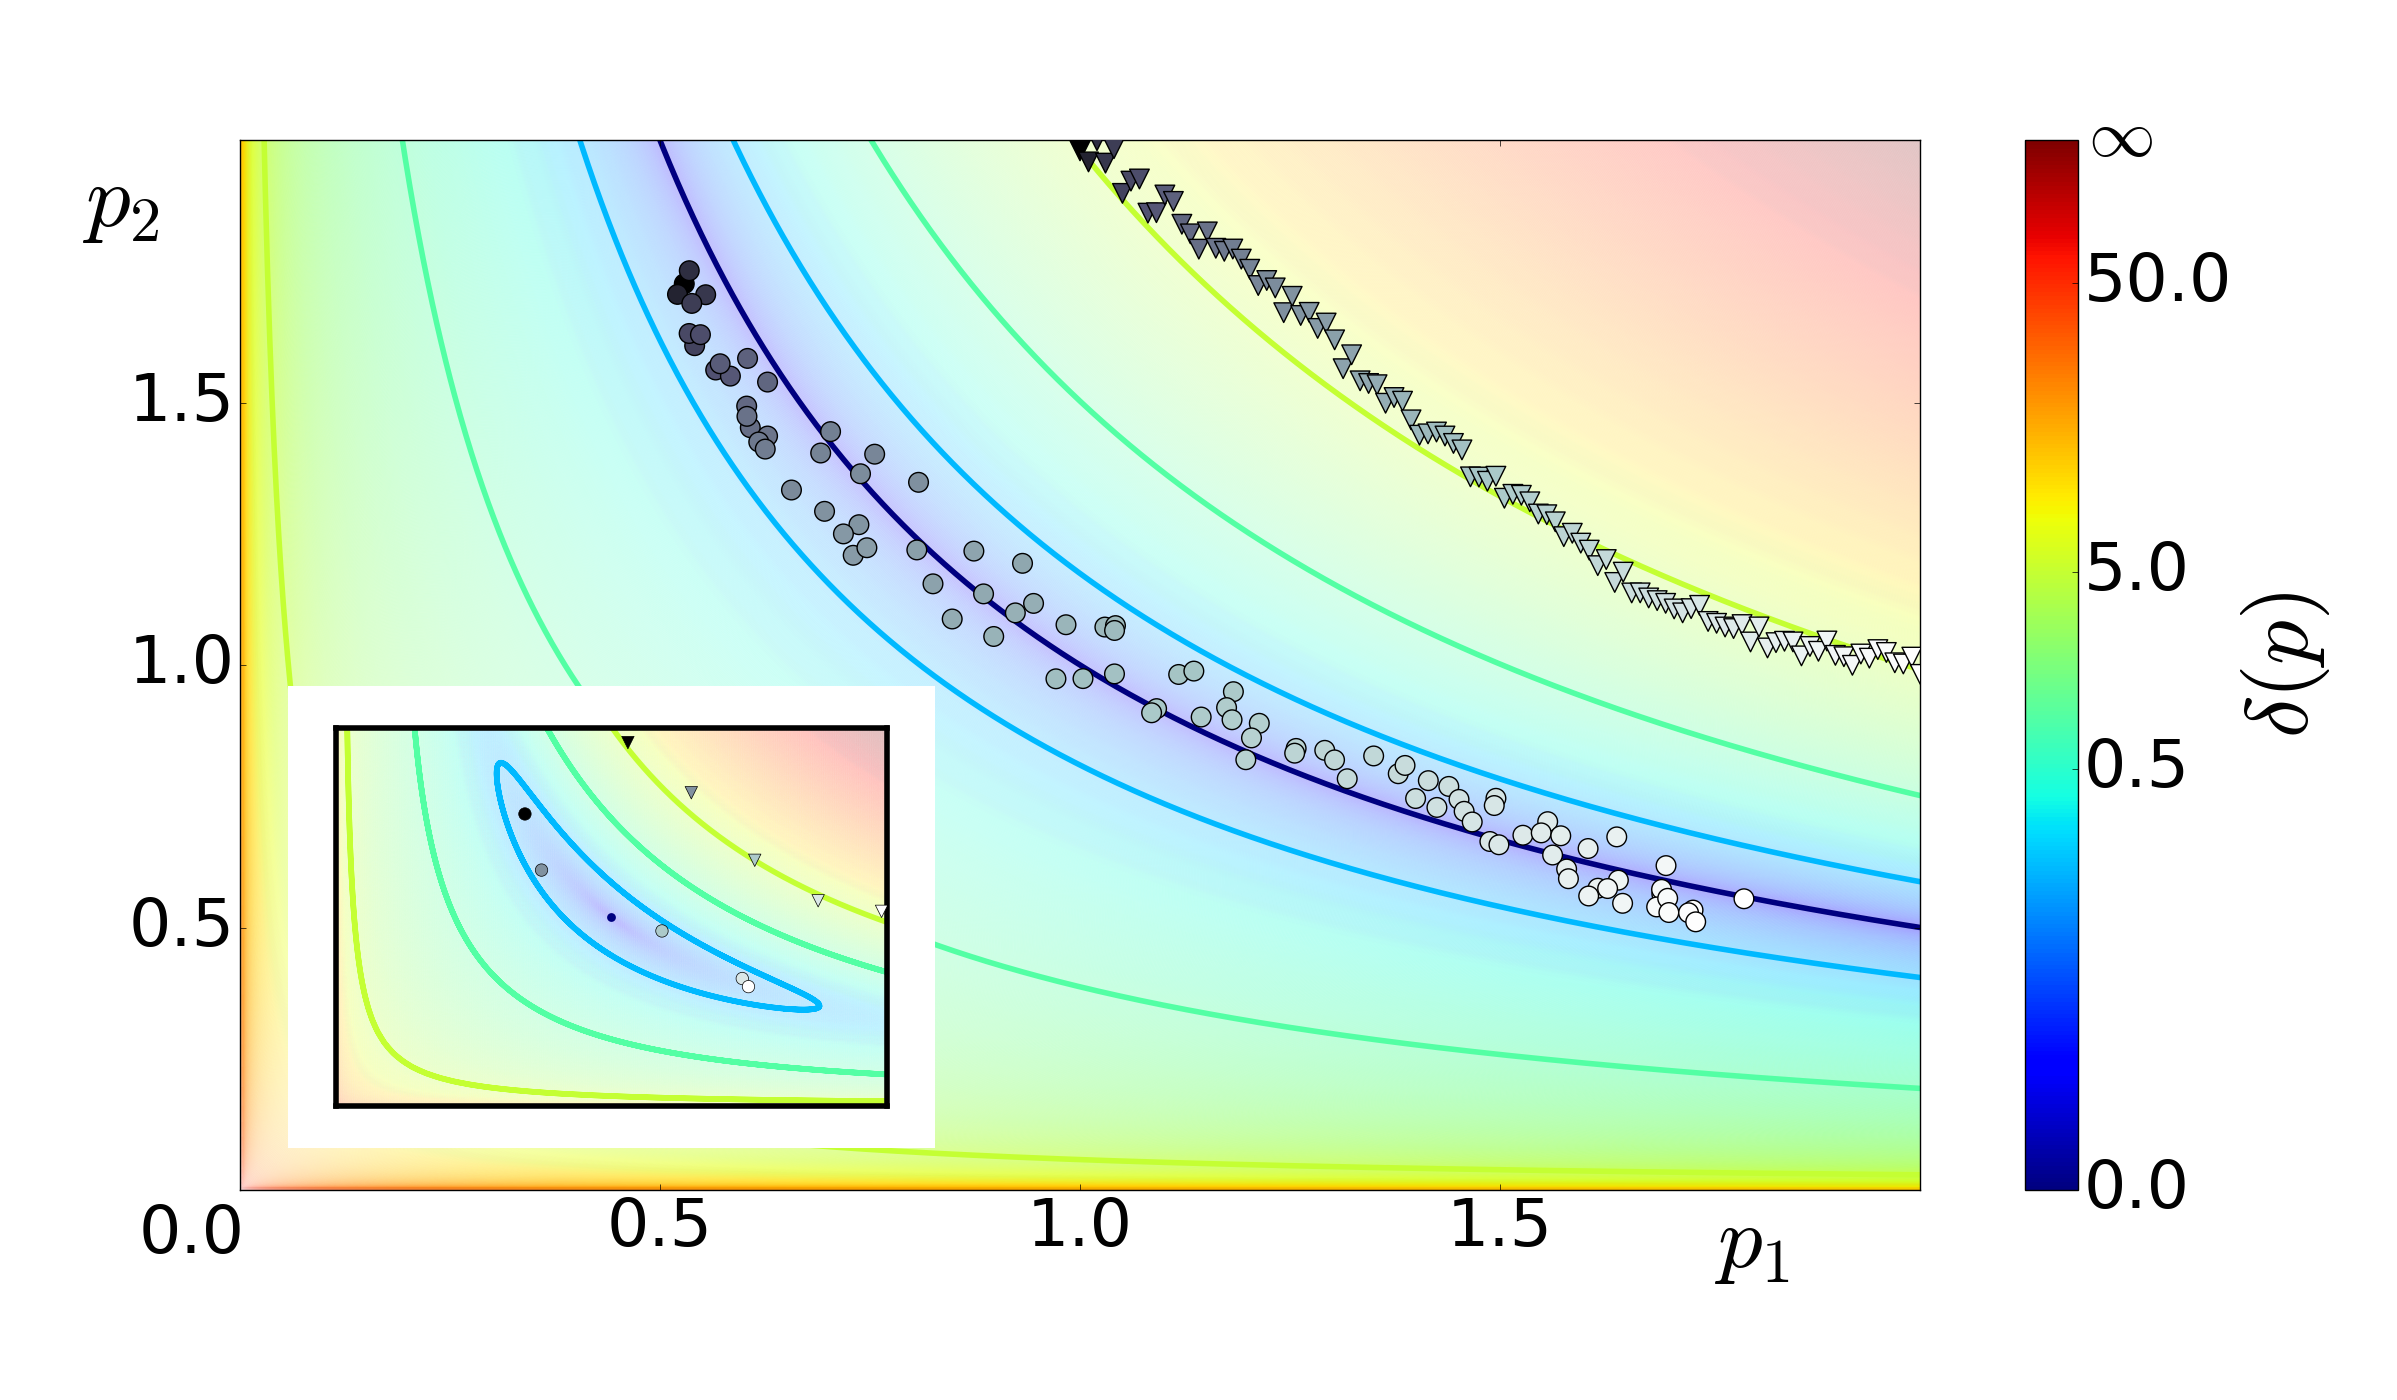
\includegraphics[width=1.0\linewidth]{p2-p1-delta}}
  \caption[Illustration of effects of sloppiness on
  optimization]{Coloring the $(p_1, p_2)$ plane by $\delta$ for
    $f(\theta) = (p_1 p_2 , \ln(p_1) + \ln(p_2) , (p_1 p_2)^2)$ (main
    figure) and the perturbed $g(p1, p2) = f(p_1, p_2) +
    \left(2*\epsilon*(p1 - p2), 0, 0\right)$ with $\epsilon = 0.2$
    (inset). $\delta$ values are calculated with respect to the base
    parameters $p^* = (1, 1)$: $\delta(p_1, p_2) = \| f(p_1, p_2) -
    f(p_1^*, p_2^*)\|$. Also shown are a range of initial and final values of
    a gradient descent algorithm. For $f$, convergence can occur
    anywhere along the infinite band for which $\delta$ is less than
    the accepted tolerance. For $g$, convergence is confined to
    bounded but stretched regions in the plane.
    \label{fig:non-id} }
\end{figure}



\section{Example from chemical kinetics} \label{sec:rr}

We now examine a system of chemical reactions in which an effective
parameter again emerges, and show how we can detect this in a
data-driven manner. The three-species system is

\begin{align}
  A
  \xrightleftharpoons[k_{-1}]{k_1}
  B
  \xrightarrow[]{k_2}
  C
  \label{mech:abc}
\end{align}

Under mass action kinetics, the concentration of the end product is
given by the analytical expression
% 
\begin{align}
  C(t|\theta)
  =
  A_0
  \left(
  \frac{k_1 k_2}{\alpha \beta}
  +
  \frac{k_1 k_2}{\alpha(\alpha - \beta)}
  e^{-\alpha t}
  -
  \frac{k_1 k_2}{\beta(\alpha - \beta)}
  e^{-\beta t}
  \right)
  \label{eq:cfull}
\end{align}
% 
where $(A_0,B_0,C_0)$ are the fixed constituent concentrations at time
zero and $\alpha,\beta$ depend on $\theta=(k_{-1},k_1,k_2)$; see
Appendix~\ref{app:abc} for the derivation. In the parameter regime
$k_1 k_2 \ll (k_1 + k_{-1} + k_2)^2$, \eqref{eq:cfull} is well
approximated by
% 
\begin{align}
  C_{eff}(t|\theta)
  =
  A_0
  \left(
  1 - e^{-k_{eff} t}
  \right) ,
  \quad
  k_{eff}
  =
  \frac{k_1 k_2}{k_{-1} + k_1 + k_2} .
  \label{eq:abc-qssa}
\end{align}
% 
Note that this approximate solution extends to a larger parameter
range the quasi-steady state approximation (QSSA)
$C_\mathrm{QSSA}(t|\theta) = A_0 (1 - e^{-k_\mathrm{QSSA} t})$, valid
for $k_1 \ll k_{-1} + k_2$ with
$k_\mathrm{QSSA}=k_1 k_2/(k_{-1} + k_2)$.  Plainly, this approximate
solution represents an effective reduction of parameter space down to
the single parameter $k_{eff}$, the levels sets of which foliate
parameter space as in Fig.~\ref{fig:abc-ill}.

To verify that $C(t)$ remains roughly constant on these level sets, we
choose reference parameter settings $\theta^*$ in the regime
identified above, fix sampling times $t_1,\ldots,t_N$, set the model
response to $f(\theta)=( C(t_1|\theta) , \ldots , C(t_N|\theta) )$,
sample log-parameter space uniformly, and record the squared Euclidean
distance $\delta(\theta) = \| f(\theta) - f(\theta^*) \|^2$ for each
sampled $\theta$.  Figure~\ref{fig:abc-keff} shows the results colored
by $k_{eff}$. We only retained parameter combinations with
$\delta(\theta) < 10^{-6}$ to aid in visualization. As expected, the
level sets of constant $\delta$ align with those of the effective
parameter, so this automated sampling process effectively reveals
sheets of different $k_{eff}$ values without recourse to an analytic
expression.

\begin{figure}[!htp]
  \centering
  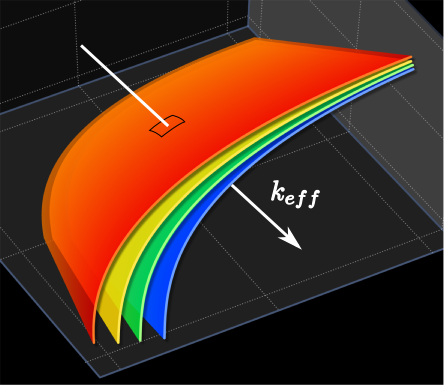
\includegraphics[width=0.4\textwidth]{keff-illustration}
  \caption[Illustration of level sets of the effective parameter in a
  model of chemical kinetics]{Illustration of level sets of $k_{eff}$
    in parameter space. \label{fig:abc-ill}}
\end{figure}


\begin{figure}[ht!]
  \centering
  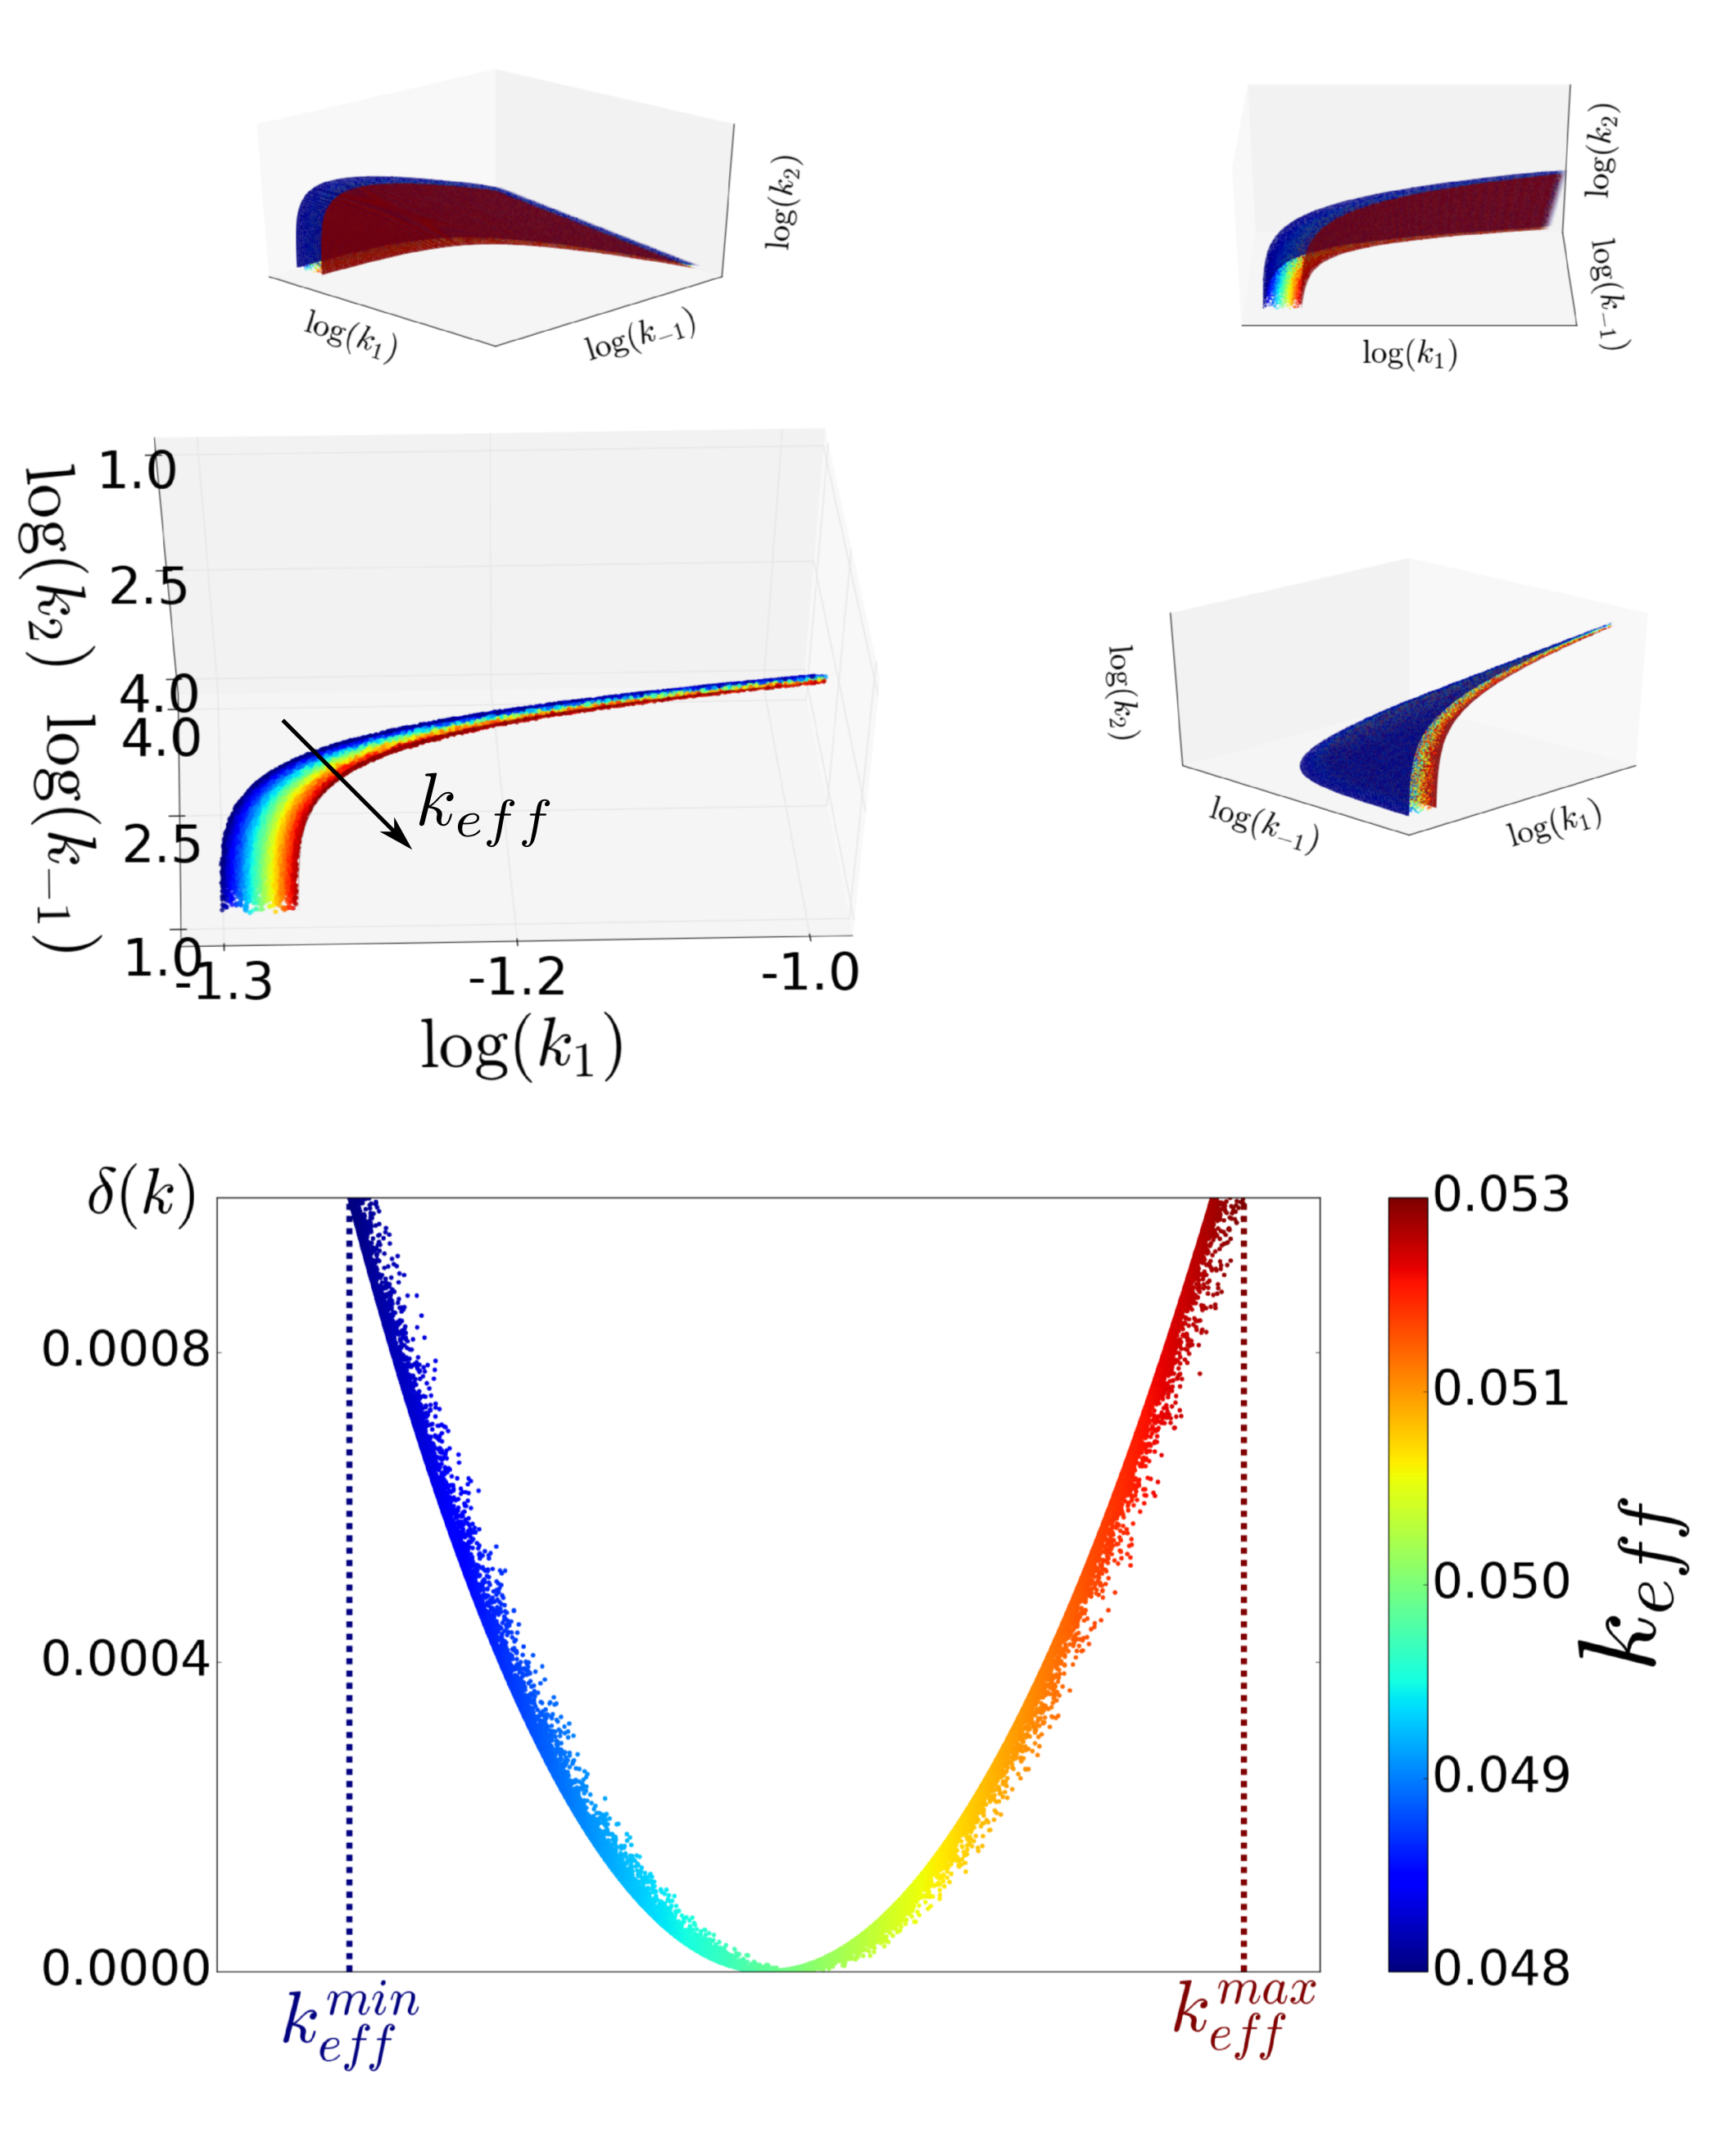
\includegraphics[width=0.9\textwidth]{keffs-delta-keff-vertical}
  \caption[Quantitative three-dimensional views of level sets of the
  effective parameter in a model of chemical kinetics]{(top) Region of
    parameter space lying within large value of $\delta = 10^{-3}$,
    colored by $k_{eff}$. Smaller rotations show three-dimensional
    structure. (bottom) Plot of $\delta$ vs $k_{eff}$ over the dataset
    showing that $\delta(k_1, k_{-1}, k_2) = \delta(k_{eff})$ as
    expected from the reduced reaction kinetics. \label{fig:abc-keff}}
\end{figure}


\begin{figure}[!htp]
  \centering
  \begin{tabular}{cc}
    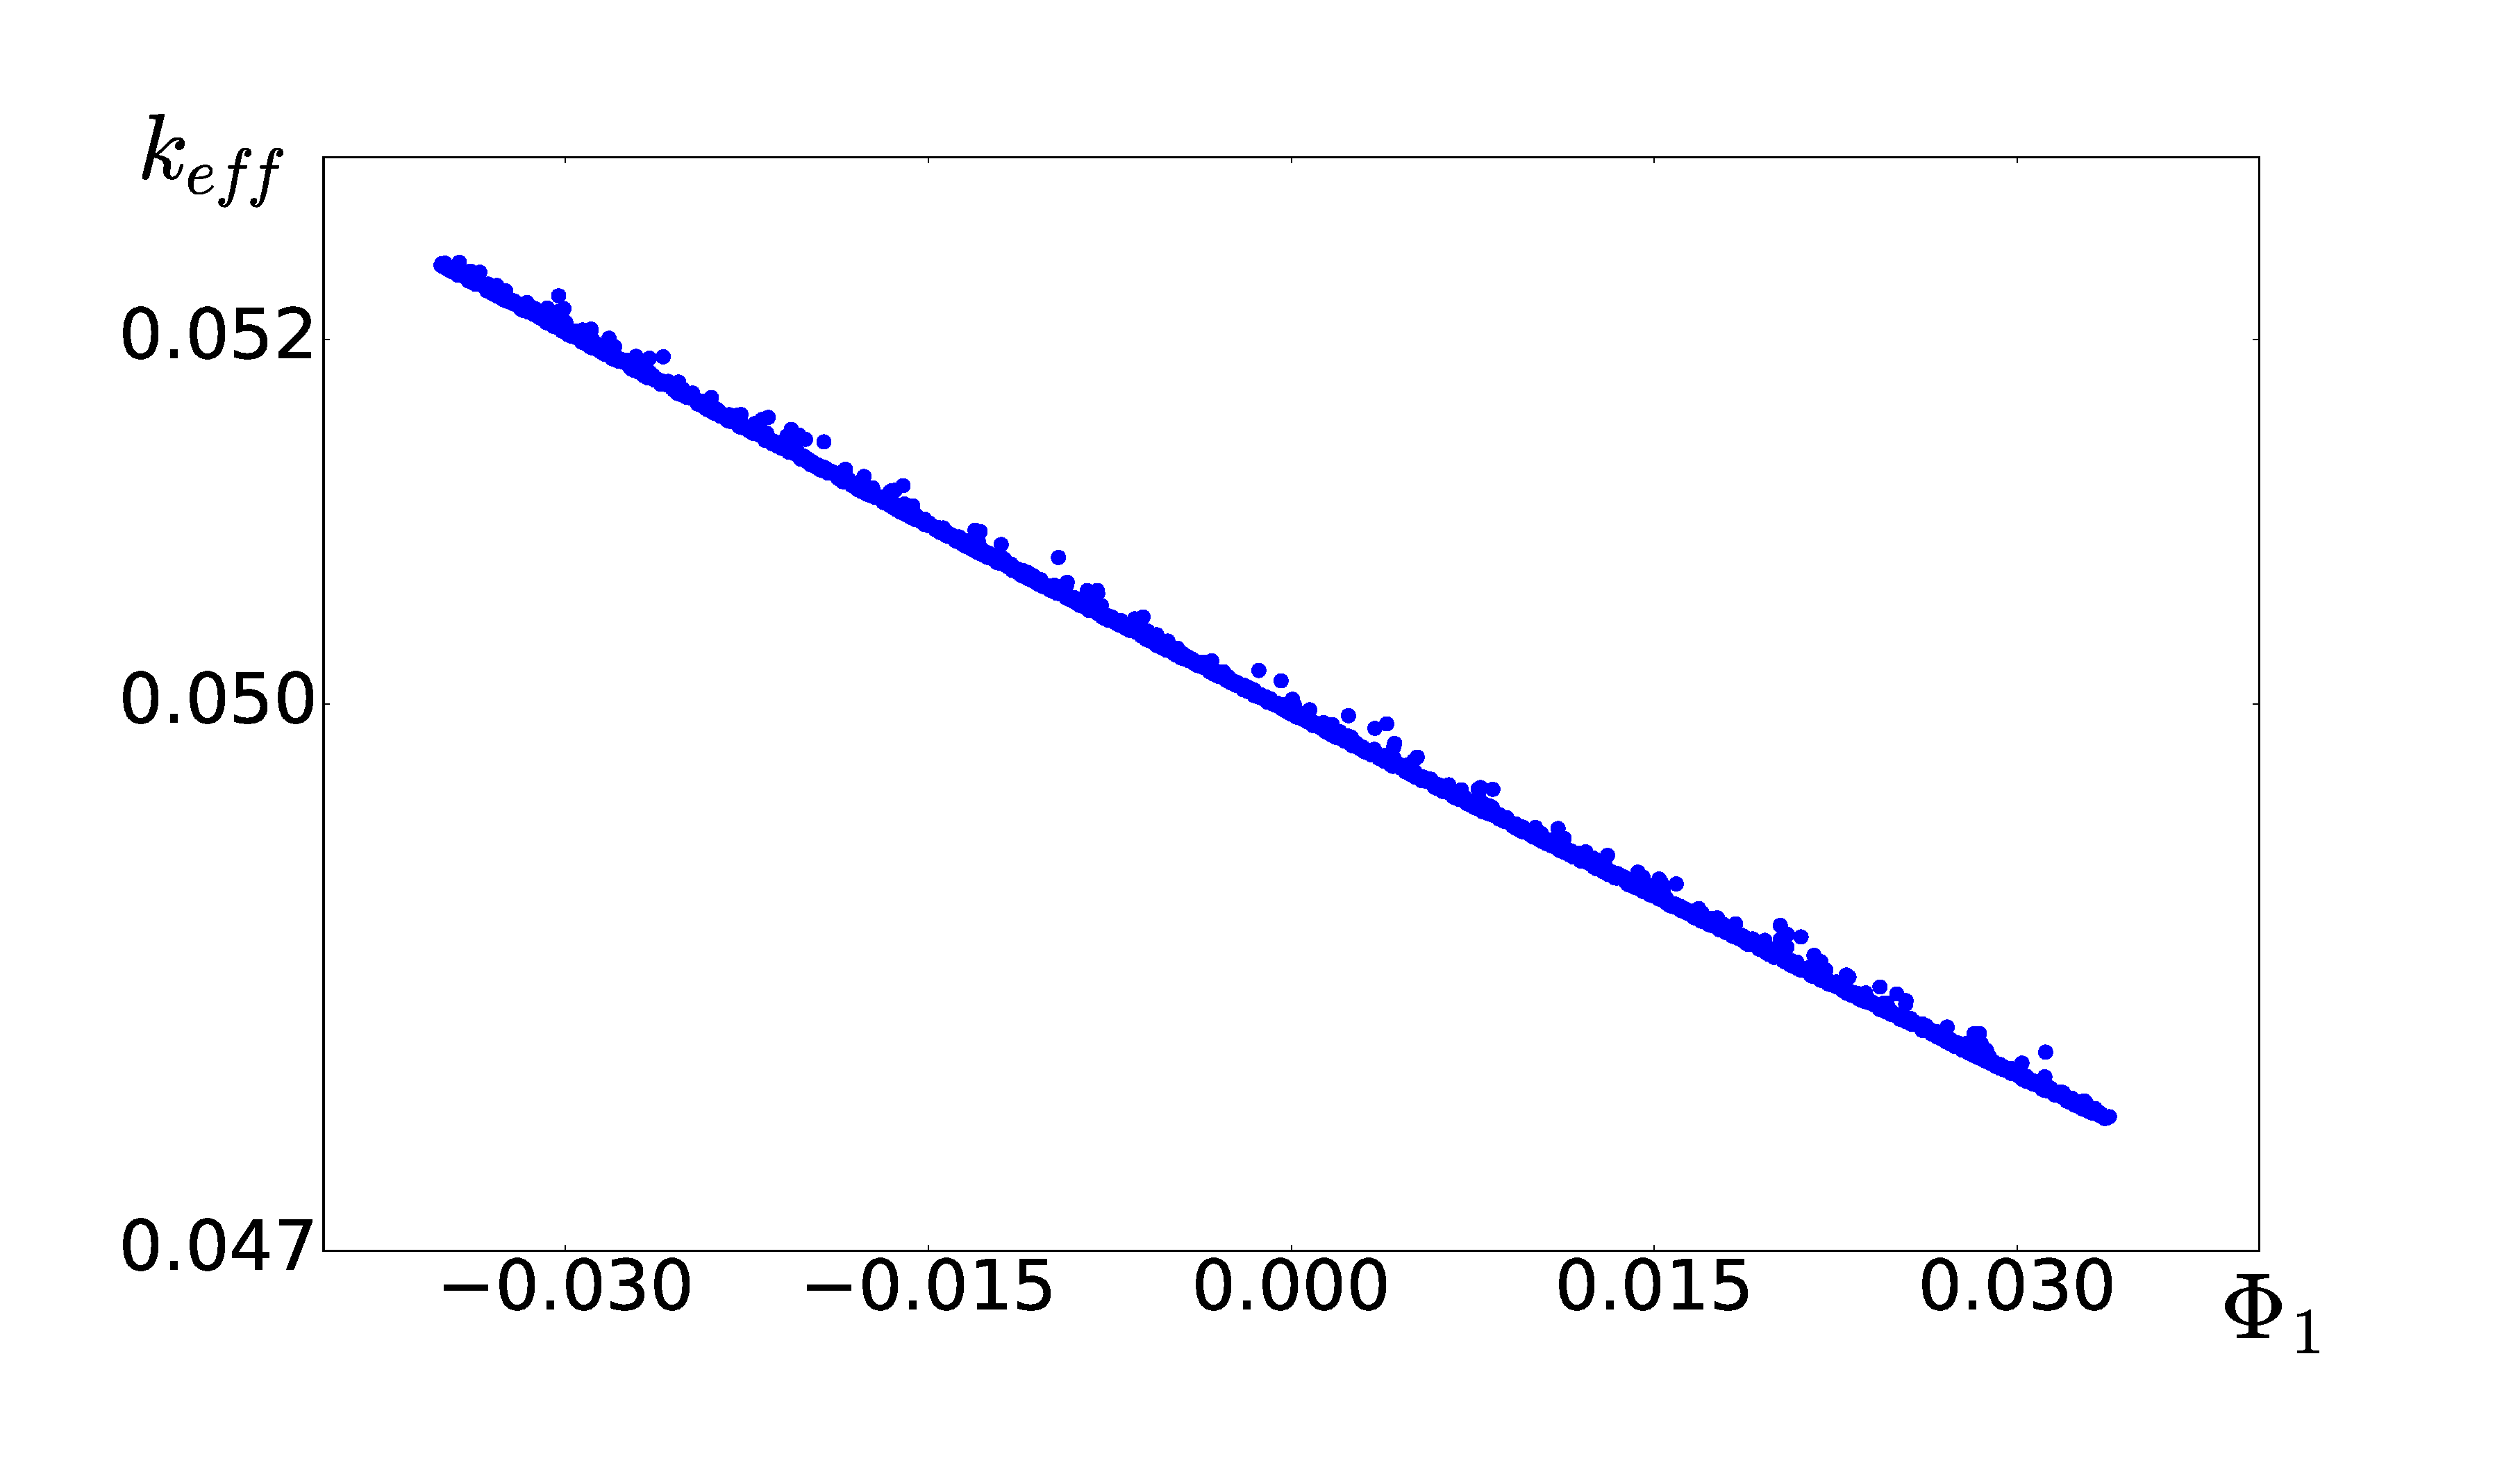
\includegraphics[width=0.45\textwidth]{keff-phi1} &
                                                        \includegraphics[width=0.5\textwidth]{k2-kinv-k1-phi1}\\
    (a) & (b)
  \end{tabular}
  \caption[DMAPS results for simple kinetic model]{(a) Coloring parameter space by $\phi_1$, showing that
    $\phi_1$ captures the effective parameter in this system; (b)
    $k_{eff}$ plotted against $\phi_1$ showing that the first DMAPS
    eigenvector parameterizes the significant, nonlinear parameter
    combination hidden in our model. \label{fig:abc-dmaps}}
\end{figure}


With this data in hand, we turn to a description of our modified
DMAPS algorithm. Details of the basic algorithm can be found in
Section~\ref{sec:dmaps}. In brief, given a collection of parameter
values ${\theta_i}_{i=1}^N$, we define our DMAPS kernel as

\begin{align}
  k(\theta_i, \theta_j) = \exp \left(-\frac{\|f(\theta_i) -
  f(\theta_j)\|^2}{\epsilon^2} \right)
  \label{eq:dmaps-mm}
\end{align}

The key point is that while the data in Figure~\ref{fig:abc-keff}
obviously represent a sample of parameter space, they simultaneously
sample the model response space through $f(\theta)$. Considering the
structure of this space, we can understand that all of the points
lying on a surface of constant $k_{eff}$ will be mapped to
approximately the same point in model response space: they share the
same output concentration trajectory as seen in
Equation~\ref{eq:abc-qssa}. Only changes in $k_{eff}$ affect the model
output, and thus our data will lie along a one-dimensional curve in
model response space, parameterized by $k_{eff}$. Therefore, if we
apply DMAPS to the model response data, the first eigenvector $\phi_1$
will yield a parameterization of this curve and we expect $k_{eff}$
and $\phi_1$ to be in one-to-one correspondence. This is precisely
what Figures~\ref{fig:abc-dmaps} shows. DMAPS has, in effect,
uncovered the effective parameter hidden in the system using only
parameter and model response data. We will now investigate how
sloppiness can arise in singularly- and regularly-perturbed systems,
and we will see that DMAPS is able to provide a more uniformly
significant reparameterization.


\section{Regular perturbation}

Let us now consider the differential equation
%
\begin{equation}
  \frac{dy}{dt} = \epsilon y^3 - y
  \quad
  y(0) = y_0 ,
  \label{1D-model-regpert}
\end{equation}
%
with $\theta = (y_0, \epsilon)$ and
$f(\theta) = \left(y(t_1), y(t_2), \dots, y(t_n) \right)$.

Unlike the previous two examples, there is no effective parameter
hidden in this system; however, our parameters affect the model output
very differently depending on their specific values. To see why this
is, consider what happens as $\eps \rightarrow 0$. The system becomes
regularly perturbed, and converges to the simpler
$\frac{dy}{dt} = -y$. Note that in this limit, $\eps$ has no influence
on the model response, and $y_0$ becomes the only significant
parameter. Again, considering the implications for the model manifold,
it is clear that for small values of $\eps$, our response will form a
one dimensional curve parameterized by $y_0$. At larger values, both
$\eps$ and $y_0$ are significant, and the manifold is
two-dimensional. Figure~\ref{fig:regpert} (a) depicts the model
manifold colored by $\eps$, and we see exactly this behavior. The red
portion of the surface, corresponding to larger $\eps$, is
two-dimensional, while the blue, with small $\eps$, is contained in a
single line at the edge of the surface. Sampling this manifold, as
detailed in Appendix~\ref{app:regpert}, and applying DMAPS with the
kernel presented in Equation~\ref{eq:dmaps-mm} yields the same
information directly from data. Figure~\ref{fig:regpert} (b) shows the
$(\eps, y_0)$ parameter plane colored by $\phi_1$. At larger values of
$\eps$ the colors vary without any significant trend as this region is
two-dimensional. However, at small $\eps$, the colors flatten out
horizontally: $\phi_1$ is constant along lines of constant
$y_0$. DMAPS captures the fact that only one direction in parameter
space is relevant in the regularly perturbed regime. To continue along
this line in a slightly more complicated scenario, our next system
will be singularly perturbed.

\begin{figure}[ht!]
  \centering
  \begin{tabular}{cc}
    \includegraphics[width=0.5\textwidth]{y3-y2-y1-eps} &
                                                           \includegraphics[width=0.5\textwidth]{y0-eps-phi1} \\
    (a) & (b)\\
  \end{tabular}
  \caption[Model manifold and parameter space of regularly perturbed system]{(a) Model manifold of regularly perturbed system with
    parameters $y_0$ and $\epsilon$, colored by $\epsilon$. As
    $\epsilon$ decreases, the model response is increasingly
    determined solely by $y_0$ as the system converges to $y' = -y$;
    (b) Parameter space colored by $\phi_1$ for the regularly
    perturbed system. As $\epsilon$ decreases, only the value of $y_0$
    is significant. This is captured by DMAPS as $\phi_1$ varies only
    vertically, in the $y_0$ direction, at small
    $\epsilon$. \label{fig:regpert}}
\end{figure}


\section{Singular perturbation}

The system is now given by

\begin{align}
  \frac{dx}{dt}&=2-x-y\\
  \frac{dy}{dt}&= \frac{1}{\epsilon}(x-y)
\end{align}    

with $\theta = (y_0, \epsilon)$ and
$f(\theta) = \left(y(t_1), y(t_2), \dots, y(t_n) \right)$ as
before. At small values of $\eps$ the equations become singularly
perturbed, and we cannot simply set $\eps = 0$ to find our reduced
description as before. Instead we see that $y$ will rapidly approach
the slow manifold $y = x$, and then progress towards the steady state
$(x,y) = (1,1)$. The phase portrait for this system is shown in
Figure~\ref{fig:singpert}.

Crucially, on the slow manifold our system is approximately
one-dimensional, governed by $\frac{dx}{dt} = -2 - 2x$. If we choose
our sampling times $t_1, t_2, \dots, t_n$ based on the slow timescale
of the system, our dynamics will be one-dimensional, and in fact
neither $\eps$ nor $y_0$ will affect the model response. At small
$\eps$, $y$ quickly converges to the slow manifold (order $\eps$
time), and then slowly evolves toward the stationary state. At
$\eps \ll 1$, our model manifold converges to a single,
zero-dimensional point. Whereas in the regularly perturbed example we
transitioned from two to one significant parameters, singular
perturbation brings a transition from two to zero. If we have obtained
a sample of the $(\eps, y_0)$ parameter plane, we can again apply
DMAPS to re-parameterize the system. Figure~\ref{fig:singpert-dmaps}
shows the results of such an analysis. In
Figures~\ref{fig:singpert-dmaps} (a) and (d) we have colored the
parameter plane by $\phi_1$ and $\phi_2$, analogous to
Figure~\ref{fig:regpert} (b). Both eigenvectors are constant at small
$\eps$ reflecting the complete absence of significant parameters in
this regime. At larger $\eps$, $\phi_1$ and $\phi_2$ vary
independently as this corresponds to the two-dimensional region of the
manifold. Both $(\eps, y_0)$ and $(\phi_1, \phi_2)$ can be used to
parameterize the system, but whereas there are distinct regions in
which $\eps$ and $y_0$ become irrelevant, $\phi_1$ and $\phi_2$ are
consistently significant. DMAPS provides an automated and improved
parameterization of the system.

To clarify the relationship between parameter space, the model
manifold and the DMAPS embedding, we plot these three views of the
singularly perturbed system in Figure~\ref{fig:singpert-patches}. We
also color four different patches and track their transformation from
one space to the next. The yellow rectangle at larger $\eps$ is mapped
to a slightly deformed rectangle in both the model manifold and DMAPS
embedding. The blue patch, which approaches the singularly perturbed
regime, becomes stretched at the tip. The red patch is compressed to
an apparently one-dimensional line, while the green patch, lying
solidly within the singularly perturbed region, is mapped to a single
point in both alternative spaces. This represents the fact that in the
limit of small $\eps$, neither $y_0$ nor $\eps$ influence the model
output: everything collapses to a zero-dimensional point.

\vspace{1cm}
\begin{figure}[!htp]
  \centering
  \includegraphics[width=0.4\textwidth]{sample_traj_sing}
  \caption[Phase portrait for singularly perturbed system]{The phase portrait of the singularly perturbed system for
    different initial conditions; solid lines: $\epsilon=0.02$, dotted
    lines are $\epsilon=0.12$. \label{fig:singpert}}
\end{figure}

\begin{figure}[!htp]
  \centering
  \begin{tabular}{ccc}
    \includegraphics[width=0.33\textwidth]{y0_eps_phi1_sing} &
                                                               \includegraphics[width=0.33\textwidth]{mod_man_epsilon} &
                                                                                                                         \includegraphics[width=0.33\textwidth]{phi2_phi1_eps_sing} \\
    (a) & (b) & (c)\\
    \includegraphics[width=0.33\textwidth]{y0_eps_phi2_sing} &
                                                               \includegraphics[width=0.33\textwidth]{mod_man_y0} &
                                                                                                                    \includegraphics[width=0.33\textwidth]{phi2_phi1_y0_sing}  \\
    (d) & (e) & (f)\\
  \end{tabular}
  \caption[DMAPS results for singularly perturbed system]{(a) and (d) Parameter space colored by $\phi_1$ and
    $\phi_2$; (b) and (e) Model manifold colored by $\epsilon$ and
    $y_0$; (c) and (f) Diffusion map space colored by $\epsilon$ and
    $y_0$ \label{fig:singpert-dmaps}}
\end{figure}


\begin{figure}[!htp]
  \centering
  \begin{tabular}{c}
    \includegraphics[height=0.2\textheight]{y0-eps-patches} \\
    (a)\\
    \includegraphics[height=0.2\textheight]{y4-y3-y2-patches}\\
    (b)\\
    \includegraphics[height=0.2\textheight]{phi2-phi1-patches}\\
    (c)\\
  \end{tabular}
  \caption[Different views of singularly perturbed system]{(a) Patches in parameter space for the singularly perturbed
    system; (b) Corresponding patches in model response space; (c)
    Corresponding patches in DMAPS embedding
    space \label{fig:singpert-patches}}
\end{figure}


\section{Application to Michaelis-Menten kinetics}

Finally, we apply our toolbox to a familiar chemical kinetic
prototype, namely the Michaelis-Menten system modeling enzymatic
action \cite{johnson_original_2011}.  In that mechanism, a substrate
$S$ is turned into product $P$ by the action of an enzyme $E$ through
the creation of an intermediate complex $C$,

\begin{align}
  E + S \xrightleftharpoons[k_{-1}]{k_1} C \xrightarrow[]{k_2} E + P
  \label{mech:mm}
\end{align}

The mechanism differs from Mechanism~\ref{mech:abc} in that the
addition of a recycled but limited enzyme supply introduces
nonlinearities into the governing system of differential equations,


\begin{align}
  \begin{split}
    S' &= -k_1 E S + k_{-1} C , \\
    C' &= k_1 E S - (k_{-1} + k_2) C , \\
    E' &= -k_1 E S + (k_{-1} + k_2) C , \\
    P' &= k_2 C
  \end{split}
\end{align}


The conservation laws $S + P + C = S_T$ and $E + C = E_T$ reduce the
number of variables by two, and we arrive at the final model

\begin{align}
  \begin{split}
    S' &= -k_1 (E_T-C) S + k_{-1} C , \\
    C' &= k_1 (E_T-C) S - (k_{-1} + k_2) C
    \label{eq:MM}
  \end{split}
\end{align}

Following the classical setting
\cite{johnson_original_2011,johnson_original_2011,segel_quasi-steady-state_1989},
we set the initial concentrations of complex and product to zero,
$C_0=P_0=0$, so that $S_0 = S_T$ and $E_0 = E_T$.  Further adapting
ideas from \cite{segel_quasi-steady-state_1989}, we recoordinatize the
parameter space through the transformations

\begin{align}
  \begin{split}
    K_M = \dst\frac{k_{-1} + k_2}{k_1} , &\quad
    V_M = k_2 E_T , \\
    \sigma = \dst\frac{S_T}{K_M} , \quad \kappa =
    \dst\frac{k_{-1}}{k_2} , &\quad \epsilon = \dst\frac{E_T}{S_T +
      K_M}
    \label{eq:param-defs}
  \end{split}
\end{align}

The observable here is the product concentration $P$ at ten equally
spaced times in the interval $[t_s/2,2t_s]$, where the timescale
$t_s = (S_T^* + K_M^*)/V_M^*$. Thus
$f:\mathbb{R}^5 \rightarrow \mathbb{R}^{10}$ maps our five
parameter values to ten points along $P$'s trajectory. Setting
reference parameter values at
$(K_M^*,V_M^*,S_T^*,\epsilon^*,\kappa) = (1,1,1,10^{-3},10)$, we
investigate the system in a manner similar to that previously
presented.  First we sample parameter settings lying within a fixed
distance $\delta=0.05$ of
$f^* = f(K_M^*, V_M^*, S_T^*, \epsilon^*,
\kappa^*)$, and then we apply the modified DMAPS algorithm to that
dataset to uncover significant parameter combinations.  Before delving
into DMAPS, however, we first probe the system with a simpler, linear
PCA analysis.  By applying this technique to the Jacobian of the model
response

\begin{align}
  \mathrm{J} = \begin{bmatrix} \frac{\partial f_1}{\partial K_M} &
    \frac{\partial f_1}{\partial V_M} & \frac{\partial f_1}{\partial
      S_T} & \frac{\partial f_1}{\partial \epsilon} & \frac{\partial
      f_1}{\partial \kappa} \\ \vdots & & & & \vdots \\ \frac{\partial
      f_N}{\partial K_M} & & \hdots & & \frac{\partial f_N}{\partial
      \kappa} \end{bmatrix}
\end{align}

and examining the coefficients of the principal components
$\mathrm{V}$ where $\mathrm{J} = \mathrm{U \Sigma V^T}$, we will
uncover, in a local, linear sense, a basis for parameter space which
better captures the directions which do and do not affect model
output. This can be observed from the fact that
$\| f(\theta + \Delta \theta) - f(\theta) \| \approx \| \mathrm{J}
\Delta \theta \| = \| \mathrm{U \Sigma V^T} \Delta \theta
\|$. When $\Delta \theta$ aligns with a principal component whose
corresponding singular value is large, it will point in a direction of
significant model response variation. Conversely, a
$\Delta \theta$ which aligns with a principal component whose
singular value is small will point in a sloppy direction along which
model response changes minimally. Examining the SVD of the Jacobian
evaluated at $\theta^*$ we find for the principal components (with
entries less than $10^{-1}$ rounded to zero and singular values
rounded to the nearest order of magnitude for clarity)

\[
  V = \begin{blockarray}{cccccc} & v_1 & v_2 & v_3 & v_4 & v_5
    \\ \begin{block}{c[ccccc]} K_M & 0.3 & \minus 0.4 & \minus 0.9 & 0
      & 0 \\ V_M & \minus 0.4 & 0.8 & \minus 0.5 & 0 & 0 \\ S_T &
      \minus 0.9 & \minus 0.5 & 0 & 0 & 0 \\ \epsilon & 0 & 0 & 0 &
      0.9 & \minus 0.5 \\ \kappa & 0 & 0 & 0 & \minus 0.5 & \minus 0.9
      \\ \end{block} & & & & & \\ \begin{block}{c[ccccc]} \sigma &
      10^0 & 10^0 & 10^{\minus 2} & 10^{\minus 5} & 10^{\minus 6}
      \\ \end{block} \end{blockarray}
\]

where the final row labeled $\sigma$ contains the corresponding
singular values. This simple analysis immediately suggests the
existence of two sloppy parameters in this regime, $\kappa$ and
$\epsilon$, as the principal components that span these axes
correspond to significantly smaller singular values compared to the
other vectors. In addition, it appears that the parameter space
direction $K_M = V_M$ may be sloppy as this approximately corresponds
to the third smallest principal component, singular value pair. With
this simple analysis in hand, we turn to computational verification of
the results using both direct numerical experiments and the DMAPS
scheme outlined above, along with supporting analytical arguments.

First we show that the direction $K_M = V_M$ is indeed sloppy so that
one cannot precisely determine both $K_M$ and $V_M$, but only their
ratio. To do so we turn to the Lineweaver-Burk plot, a graphical
procedure allowing one to determine $K_M$ and $V_M$ from experimental
data of the reaction rate and substrate concentration evolution over
time \cite{lineweaver_determination_1934}. By generating many noisy realizations of the product
concentration profiles as one might collect experimentally in the lab
and then fitting each with the Lineweaver-Burk method, we can observe
the range of predicted $K_M$, $V_M$ pairs. These results are plotted
in Fig.~\ref{fig:lb}. In a typical setting we would expect a spread of
predicted values centered around the true, zero-noise parameters
taking the shape of some ellipsoid. However, as we have seen in
previous examples, in the presence of sloppiness this ellipsoid would
be stretched out along the sloppy parameter direction. This is
precisely what we find in Fig.~\ref{fig:lb}: so long as the ratio
$K_M/V_M = K_M^*/V_M^* = 1$, a wide range of values provide best-fit
parameters in the presence of slight noise. Therefore, when fitting
parameters in this regime, we must accept that we may not be able to
determine precise values of both $K_M$ and $V_M$.


\begin{figure}
  \centering
  \includegraphics[width=1.0\linewidth]{k-v-lb}
  \caption[Lineweaver-Burk fitting results]{Best fit $K_M$ and $V_M$ values for many noisy
    concentration trajectories (blue dots). Sloppiness is evident in
    the spread of the data along the line $K_M/V_M = 1$ (plotted in
    red for reference). \label{fig:lb} }
\end{figure}

Next, we examine the system using DMAPS. We use the five-dimensional
dataset obtained by sampling parameter space around $\theta^*$ and
keeping those points for which
$\|f(\theta) - f(\theta^*) || < 5 \cdot 10^{-2}$, and apply DMAPS
with an $\epsilon$ value of $10^{-1}$.

Having computed our DMAP eigenvectors, it remains to determine which
of them correspond to independent directions in parameter space, as
certain eigenvectors may parameterize the same directions (see
\cite{dsilva_parsimonious_2015} for details). Using the algorithm
developed in \cite{dsilva_parsimonious_2015}, we compute a residual
for each eigenvector which, roughly speaking, assesses how much new
information it contains. The results shown in Fig~\ref{fig:resids}
suggest that eigenvectors $\phi_1$ and $\phi_2$ parameterize
independent directions. Our previous analysis would then suggest that
$\phi_1$ and $\phi_2$ correspond to important parameter directions,
and would provide a good set of coordinates on our model manifold.

We can test this hypothesis by projecting the model manifold onto two
axes, here $f_1$ and $f_{10}$, and coloring the result by our
eigenvectors. If the colors vary smoothly over the points, we have
uncovered an eigenvector that parameterizes the manifold. These
colorings are provided in Fig.~\ref{fig:mm-dmaps}. Based on these
figures, we can conclude that indeed $\phi_1$ and $\phi_2$ provide
coordinates along the model manifold. The sloppiness in $K_M/V_M$ was
discussed in the previous paragraph, but it remains to show why we
would lose two more parameters. In fact, as $\epsilon \rightarrow 0$,
the set of differential equations given in \eqref{eq:MM} become
singularly perturbed. In this limit, the leading order dynamics are
not influenced by $\kappa$, as shown in
\cite{segel_quasi-steady-state_1989}. Thus, for small enough
$\epsilon$, we will lose our ability to determine both $\epsilon$ and
$\kappa$. This is precisely what is reflected in our DMAPS results.

\begin{figure}[!htp]
  \centering
  \begin{tabular}{cc}
    \includegraphics[width=0.5\textwidth]{f10-f1-phi1} &
    \includegraphics[width=0.5\textwidth]{f10-f1-phi2}\\
    (a) & (b) \\
  \end{tabular}
  \caption[DMAPS results for Michaelis-Menten system I]{Projection of the model manifold onto $f_1$ and $f_{10}$
    colored by different DMAP eigenvectors. As $\phi_1$ and $\phi_2$
    vary smoothly over the surface and parameterize independent
    directions, these eigenvectors offer a good pair of coordinates on
    the manifold \label{fig:mm-dmaps}}
\end{figure}


\begin{figure}[ht!]
  \centering
  \includegraphics[width=\textwidth]{vm-st-km-all}
  \caption[DMAPS results for Michaelis-Menten system II]{(left) Scatter-plot of points in parameter space such that
    $\|f(\theta) - f^*\| < \delta$. This reveals a sloppy direction
    corresponding to the long, curved axis, and two significant
    directions orthogonal to it. (right) Two-dimensional cross section
    colored by $\phi_1$ and $\phi_2$. As expected, these eigenvectors
    do parameterize the significant directions in parameter space.
    \label{fig:mm-all} }
\end{figure}

\begin{figure}
  \centering
  \includegraphics[width=0.6\linewidth]{residuals}
  \caption[DMAPS residuals from Michaelis-Menten system]{Residuals computed as described in previous section. High
    residuals for a given eigenvector suggest that it is not a
    function of previous eigenvectors, and thus contains new
    information. This plot suggests five significant eigenvectors, the
    first two of which parameterize significant parameter directions,
    while the final three capture sloppy
    directions. \label{fig:resids} }
\end{figure}

\section{Discussion}

The examples presented throughout this chapter show that DMAPS
consistently provides a good parameterization of the model of
interest. This parameterization is often more useful than the natural
parameter combinations originally used to formulate the system, as
DMAPS automatically accounts for regions of singular- and
regular-perturbation, in addition to detecting hidden effective
parameters. This opens the door to a number of applications, while
also inviting further research to improve certain aspects of the
method.

As we discussed in the introduction, one of the hallmarks of
sloppiness is slow convergence of model-fitting routines
\cite{transtrum_geometry_2011}. The algorithms become trapped in
sloppy regions of parameter space in which model response is nearly
constant. Thus, an obvious use of our technique would be to accelerate
these fitting procedures. The idea would be to take steps in the
DMAPS-embedding space instead of along the natural parameters. This
would require an ability to sample patches of the model manifold on
demand, and to perform extrapolation in DMAPS space. Thankfully,
results along these directions have already been established, and
these could likely be adapted to this particular setting
\cite{chiavazzo_intrinsic_2017}. We would also need the ability to map
DMAPS coordinates back to points on the model manifold. This is
related to the problem of ``lifting'' in the Equation Free framework,
again an area where existing work may be quickly incorporated
\cite{rajendran_data_2016,laing_equation-free_2015,laing_coarse-grained_2007}.

Another avenue would be nonlinear sensitivity analysis. The
simplest and most common methods simply vary individual parameters
while observing changes in model output
\cite{murphy_quantification_2004}. The shortcomings of such studies
are well known \cite{saltelli_how_2010},
but even more sophisticated methods designed for nonlinear models
assume that each parameter can be treated independently of the
others \cite{cukier_nonlinear_1978}. It would clearly be useful to
adapt this technique to the task. A simple start would be to assess
how many significant parameters a system has based on the dimension of
the DMAPS embedding \cite{dsilva_parsimonious_2015}.

Finally, further work is needed to accelerate sampling on the model
manifold. The current approach, approximate Bayesian computation, is
simple to implement but scales poorly with the dimension of parameter
space, $k$ \cite{turner_tutorial_2012}. One possibility would be to
calculate the convex hull or alpha-shape of a small sample, and then
interpolate among these points
\cite{barber_quickhull_1996,edelsbrunner_three-dimensional_1994}. Overall,
this chapter presents a novel, data-driven method to parameterize
complex models that will hopefully form the foundation for future,
practical applications.


%%% Local Variables: ***
%%% mode:latex ***
%%% TeX-master: "../../thesis.tex"  ***
%%% End: ***



% Make the bibliography single spaced
\singlespacing
\bibliographystyle{plain}

% add the Bibliography to the Table of Contents
\cleardoublepage
\ifdefined\phantomsection
  \phantomsection  % makes hyperref recognize this section properly for pdf link
\else
\fi
\addcontentsline{toc}{chapter}{Bibliography}

% % include your .bib file
\bibliographystyle{abbrv} \bibliography{./references.bib}

\end{document}

